\documentclass[10pt,journal,a4paper]{IEEEtran}

\ifdefined\pdfsuppressptexinfo\pdfsuppressptexinfo=-1\fi

\usepackage[T1]{fontenc}
\usepackage[utf8]{inputenc}
\usepackage{graphicx}
\usepackage{amsmath}
\usepackage{amssymb}
\usepackage{array}
\usepackage{booktabs}
\usepackage{longtable}
\usepackage{url}
\usepackage{xurl}
\usepackage{xspace}
\usepackage{xcolor}
\usepackage{fvextra}
\usepackage[hidelinks]{hyperref}

\newcommand{\ReviewPubid}{}
\newcommand{\MtName}{Rectina m3}
\newcommand{\MfName}{Rectina m4}
\newcommand{\DataAttribution}{The scan data were obtained from the Vesuvius Challenge data server (dl.ash2txt.org) under the data licence of the Vesuvius Challenge (LICENSE.txt).}
\newcommand{\OrgQuoteOne}{``detecting or segmenting the ink signal on, or near, the recovered writing surface''}
\newcommand{\OrgQuoteTwo}{``The subtle differences that distinguish ink from papyrus must be teased out of data like this''}
\newcommand{\RdrQuoteOne}{``Reader V3 is Reader v2 trained further on larger tiles, 30k iterations at 256 px and then 20k at 384 px''}
\newcommand{\RdrQuoteTwo}{``The architecture, the training data and the labels stayed the same''}
\newcommand{\HeldN}{8}
\newcommand{\MtHeldMeanOwnAuc}{0.8532}
\newcommand{\MtHeldMeanOwnThin}{0.8625}
\newcommand{\MtHeldMeanOwnFaEighty}{0.2582}
\newcommand{\MtHeldMeanOwnFaNinety}{0.4283}
\newcommand{\MtHeldMeanOwnLit}{0.0065}
\newcommand{\MtHeldMeanRTwoAuc}{0.8421}
\newcommand{\MtHeldMeanRTwoThin}{0.8517}
\newcommand{\MtHeldMeanRTwoFaEighty}{0.2865}
\newcommand{\MtHeldMeanRTwoFaNinety}{0.4663}
\newcommand{\MtHeldMeanRTwoLit}{0.0058}
\newcommand{\MtHeldMeanRThreeAuc}{0.8547}
\newcommand{\MtHeldMeanRThreeThin}{0.8632}
\newcommand{\MtHeldMeanRThreeFaEighty}{0.2585}
\newcommand{\MtHeldMeanRThreeFaNinety}{0.4350}
\newcommand{\MtHeldMeanRThreeLit}{0.0094}
\newcommand{\MtHeldMeanDiffTwoAuc}{+0.0111}
\newcommand{\MtHeldMeanDiffTwoThin}{+0.0107}
\newcommand{\MtHeldMeanDiffTwoFaEighty}{-0.0283}
\newcommand{\MtHeldMeanDiffThreeAuc}{-0.0015}
\newcommand{\MtHeldMeanDiffThreeThin}{-0.0007}
\newcommand{\MtHeldMeanDiffThreeFaEighty}{-0.0002}
\newcommand{\MtHeldMedianOwnAuc}{0.8569}
\newcommand{\MtHeldMedianOwnThin}{0.8694}
\newcommand{\MtHeldMedianOwnFaEighty}{0.2648}
\newcommand{\MtHeldMedianOwnFaNinety}{0.4325}
\newcommand{\MtHeldMedianOwnLit}{0.0033}
\newcommand{\MtHeldMedianRTwoAuc}{0.8435}
\newcommand{\MtHeldMedianRTwoThin}{0.8561}
\newcommand{\MtHeldMedianRTwoFaEighty}{0.2768}
\newcommand{\MtHeldMedianRTwoFaNinety}{0.4537}
\newcommand{\MtHeldMedianRTwoLit}{0.0012}
\newcommand{\MtHeldMedianRThreeAuc}{0.8503}
\newcommand{\MtHeldMedianRThreeThin}{0.8594}
\newcommand{\MtHeldMedianRThreeFaEighty}{0.2917}
\newcommand{\MtHeldMedianRThreeFaNinety}{0.4686}
\newcommand{\MtHeldMedianRThreeLit}{0.0042}
\newcommand{\MtHeldMedianDiffTwoAuc}{+0.0115}
\newcommand{\MtHeldMedianDiffTwoThin}{+0.0095}
\newcommand{\MtHeldMedianDiffTwoFaEighty}{-0.0314}
\newcommand{\MtHeldMedianDiffThreeAuc}{-0.0033}
\newcommand{\MtHeldMedianDiffThreeThin}{-0.0024}
\newcommand{\MtHeldMedianDiffThreeFaEighty}{-0.0149}
\newcommand{\MtHeldAboveTwo}{6}
\newcommand{\MtHeldKTextTwo}{6 of 8}
\newcommand{\MtBelowListHeldTwo}{0009B$\cdot$140325, 0343P$\cdot$233748-0}
\newcommand{\MtHeldFaLessTwo}{7 of 8}
\newcommand{\MtHeldAboveThree}{4}
\newcommand{\MtHeldKTextThree}{4 of 8}
\newcommand{\MtBelowListHeldThree}{0009B$\cdot$125754, 0009B$\cdot$140325, 0500P2$\cdot$055229, 0500P2$\cdot$055230}
\newcommand{\MtHeldFaLessThree}{5 of 8}
\newcommand{\CtrlN}{6}
\newcommand{\MtCtrlMeanOwnAuc}{0.8476}
\newcommand{\MtCtrlMeanOwnThin}{0.8722}
\newcommand{\MtCtrlMeanOwnFaEighty}{0.2449}
\newcommand{\MtCtrlMeanOwnFaNinety}{0.4306}
\newcommand{\MtCtrlMeanOwnLit}{0.0511}
\newcommand{\MtCtrlMeanRTwoAuc}{0.8456}
\newcommand{\MtCtrlMeanRTwoThin}{0.8698}
\newcommand{\MtCtrlMeanRTwoFaEighty}{0.2489}
\newcommand{\MtCtrlMeanRTwoFaNinety}{0.4315}
\newcommand{\MtCtrlMeanRTwoLit}{0.0416}
\newcommand{\MtCtrlMeanRThreeAuc}{0.8566}
\newcommand{\MtCtrlMeanRThreeThin}{0.8805}
\newcommand{\MtCtrlMeanRThreeFaEighty}{0.2288}
\newcommand{\MtCtrlMeanRThreeFaNinety}{0.4082}
\newcommand{\MtCtrlMeanRThreeLit}{0.0625}
\newcommand{\MtCtrlMeanDiffTwoAuc}{+0.0020}
\newcommand{\MtCtrlMeanDiffTwoThin}{+0.0024}
\newcommand{\MtCtrlMeanDiffTwoFaEighty}{-0.0039}
\newcommand{\MtCtrlMeanDiffThreeAuc}{-0.0090}
\newcommand{\MtCtrlMeanDiffThreeThin}{-0.0083}
\newcommand{\MtCtrlMeanDiffThreeFaEighty}{+0.0161}
\newcommand{\MtCtrlMedianOwnAuc}{0.8526}
\newcommand{\MtCtrlMedianOwnThin}{0.8775}
\newcommand{\MtCtrlMedianOwnFaEighty}{0.2439}
\newcommand{\MtCtrlMedianOwnFaNinety}{0.4217}
\newcommand{\MtCtrlMedianOwnLit}{0.0557}
\newcommand{\MtCtrlMedianRTwoAuc}{0.8492}
\newcommand{\MtCtrlMedianRTwoThin}{0.8736}
\newcommand{\MtCtrlMedianRTwoFaEighty}{0.2534}
\newcommand{\MtCtrlMedianRTwoFaNinety}{0.4275}
\newcommand{\MtCtrlMedianRTwoLit}{0.0493}
\newcommand{\MtCtrlMedianRThreeAuc}{0.8561}
\newcommand{\MtCtrlMedianRThreeThin}{0.8807}
\newcommand{\MtCtrlMedianRThreeFaEighty}{0.2409}
\newcommand{\MtCtrlMedianRThreeFaNinety}{0.4083}
\newcommand{\MtCtrlMedianRThreeLit}{0.0707}
\newcommand{\MtCtrlMedianDiffTwoAuc}{-0.0022}
\newcommand{\MtCtrlMedianDiffTwoThin}{-0.0019}
\newcommand{\MtCtrlMedianDiffTwoFaEighty}{-0.0081}
\newcommand{\MtCtrlMedianDiffThreeAuc}{-0.0077}
\newcommand{\MtCtrlMedianDiffThreeThin}{-0.0103}
\newcommand{\MtCtrlMedianDiffThreeFaEighty}{+0.0075}
\newcommand{\MtCtrlAboveTwo}{3}
\newcommand{\MtCtrlKTextTwo}{3 of 6}
\newcommand{\MtBelowListCtrlTwo}{0343, 0841 w00, 1447 w058}
\newcommand{\MtCtrlFaLessTwo}{4 of 6}
\newcommand{\MtCtrlAboveThree}{2}
\newcommand{\MtCtrlKTextThree}{2 of 6}
\newcommand{\MtBelowListCtrlThree}{0343, 0841 w00, 1447 w058, 1447 w060}
\newcommand{\MtCtrlFaLessThree}{1 of 6}
\newcommand{\OrgN}{4}
\newcommand{\MtOrgMeanOwnAuc}{0.8639}
\newcommand{\MtOrgMeanOwnThin}{0.8824}
\newcommand{\MtOrgMeanOwnFaEighty}{0.1982}
\newcommand{\MtOrgMeanOwnFaNinety}{0.3724}
\newcommand{\MtOrgMeanOwnLit}{0.0684}
\newcommand{\MtOrgMeanRTwoAuc}{0.8596}
\newcommand{\MtOrgMeanRTwoThin}{0.8767}
\newcommand{\MtOrgMeanRTwoFaEighty}{0.2000}
\newcommand{\MtOrgMeanRTwoFaNinety}{0.3740}
\newcommand{\MtOrgMeanRTwoLit}{0.0569}
\newcommand{\MtOrgMeanRThreeAuc}{0.8736}
\newcommand{\MtOrgMeanRThreeThin}{0.8897}
\newcommand{\MtOrgMeanRThreeFaEighty}{0.1742}
\newcommand{\MtOrgMeanRThreeFaNinety}{0.3388}
\newcommand{\MtOrgMeanRThreeLit}{0.0764}
\newcommand{\MtOrgMeanDiffTwoAuc}{+0.0043}
\newcommand{\MtOrgMeanDiffTwoThin}{+0.0056}
\newcommand{\MtOrgMeanDiffTwoFaEighty}{-0.0019}
\newcommand{\MtOrgMeanDiffThreeAuc}{-0.0097}
\newcommand{\MtOrgMeanDiffThreeThin}{-0.0073}
\newcommand{\MtOrgMeanDiffThreeFaEighty}{+0.0240}
\newcommand{\MtOrgMedianOwnAuc}{0.8628}
\newcommand{\MtOrgMedianOwnThin}{0.8813}
\newcommand{\MtOrgMedianOwnFaEighty}{0.2159}
\newcommand{\MtOrgMedianOwnFaNinety}{0.3774}
\newcommand{\MtOrgMedianOwnLit}{0.0653}
\newcommand{\MtOrgMedianRTwoAuc}{0.8588}
\newcommand{\MtOrgMedianRTwoThin}{0.8751}
\newcommand{\MtOrgMedianRTwoFaEighty}{0.2145}
\newcommand{\MtOrgMedianRTwoFaNinety}{0.3630}
\newcommand{\MtOrgMedianRTwoLit}{0.0535}
\newcommand{\MtOrgMedianRThreeAuc}{0.8784}
\newcommand{\MtOrgMedianRThreeThin}{0.8934}
\newcommand{\MtOrgMedianRThreeFaEighty}{0.1799}
\newcommand{\MtOrgMedianRThreeFaNinety}{0.2988}
\newcommand{\MtOrgMedianRThreeLit}{0.0714}
\newcommand{\MtOrgMedianDiffTwoAuc}{+0.0040}
\newcommand{\MtOrgMedianDiffTwoThin}{+0.0055}
\newcommand{\MtOrgMedianDiffTwoFaEighty}{-0.0040}
\newcommand{\MtOrgMedianDiffThreeAuc}{-0.0074}
\newcommand{\MtOrgMedianDiffThreeThin}{-0.0052}
\newcommand{\MtOrgMedianDiffThreeFaEighty}{+0.0131}
\newcommand{\MtOrgAboveTwo}{2}
\newcommand{\MtOrgKTextTwo}{2 of 4}
\newcommand{\MtBelowListOrgTwo}{0343, 0841 w00}
\newcommand{\MtOrgFaLessTwo}{2 of 4}
\newcommand{\MtOrgAboveThree}{2}
\newcommand{\MtOrgKTextThree}{2 of 4}
\newcommand{\MtBelowListOrgThree}{0343, 0841 w00}
\newcommand{\MtOrgFaLessThree}{0 of 4}
\newcommand{\AllN}{14}
\newcommand{\MtAllMeanOwnAuc}{0.8508}
\newcommand{\MtAllMeanOwnThin}{0.8666}
\newcommand{\MtAllMeanOwnFaEighty}{0.2525}
\newcommand{\MtAllMeanOwnFaNinety}{0.4293}
\newcommand{\MtAllMeanOwnLit}{0.0256}
\newcommand{\MtAllMeanRTwoAuc}{0.8436}
\newcommand{\MtAllMeanRTwoThin}{0.8595}
\newcommand{\MtAllMeanRTwoFaEighty}{0.2704}
\newcommand{\MtAllMeanRTwoFaNinety}{0.4514}
\newcommand{\MtAllMeanRTwoLit}{0.0212}
\newcommand{\MtAllMeanRThreeAuc}{0.8555}
\newcommand{\MtAllMeanRThreeThin}{0.8706}
\newcommand{\MtAllMeanRThreeFaEighty}{0.2458}
\newcommand{\MtAllMeanRThreeFaNinety}{0.4235}
\newcommand{\MtAllMeanRThreeLit}{0.0322}
\newcommand{\MtAllMeanDiffTwoAuc}{+0.0072}
\newcommand{\MtAllMeanDiffTwoThin}{+0.0071}
\newcommand{\MtAllMeanDiffTwoFaEighty}{-0.0179}
\newcommand{\MtAllMeanDiffThreeAuc}{-0.0047}
\newcommand{\MtAllMeanDiffThreeThin}{-0.0040}
\newcommand{\MtAllMeanDiffThreeFaEighty}{+0.0068}
\newcommand{\MtAllMedianOwnAuc}{0.8526}
\newcommand{\MtAllMedianOwnThin}{0.8730}
\newcommand{\MtAllMedianOwnFaEighty}{0.2510}
\newcommand{\MtAllMedianOwnFaNinety}{0.4234}
\newcommand{\MtAllMedianOwnLit}{0.0118}
\newcommand{\MtAllMedianRTwoAuc}{0.8441}
\newcommand{\MtAllMedianRTwoThin}{0.8567}
\newcommand{\MtAllMedianRTwoFaEighty}{0.2689}
\newcommand{\MtAllMedianRTwoFaNinety}{0.4391}
\newcommand{\MtAllMedianRTwoLit}{0.0082}
\newcommand{\MtAllMedianRThreeAuc}{0.8532}
\newcommand{\MtAllMedianRThreeThin}{0.8660}
\newcommand{\MtAllMedianRThreeFaEighty}{0.2673}
\newcommand{\MtAllMedianRThreeFaNinety}{0.4336}
\newcommand{\MtAllMedianRThreeLit}{0.0233}
\newcommand{\MtAllMedianDiffTwoAuc}{+0.0089}
\newcommand{\MtAllMedianDiffTwoThin}{+0.0082}
\newcommand{\MtAllMedianDiffTwoFaEighty}{-0.0129}
\newcommand{\MtAllMedianDiffThreeAuc}{-0.0077}
\newcommand{\MtAllMedianDiffThreeThin}{-0.0092}
\newcommand{\MtAllMedianDiffThreeFaEighty}{+0.0049}
\newcommand{\MtAllAboveTwo}{9}
\newcommand{\MtAllKTextTwo}{9 of 14}
\newcommand{\MtBelowListAllTwo}{0343, 0841 w00, 1447 w058, 0009B$\cdot$140325, 0343P$\cdot$233748-0}
\newcommand{\MtAllFaLessTwo}{11 of 14}
\newcommand{\MtAllAboveThree}{6}
\newcommand{\MtAllKTextThree}{6 of 14}
\newcommand{\MtBelowListAllThree}{0343, 0841 w00, 1447 w058, 1447 w060, 0009B$\cdot$125754, 0009B$\cdot$140325, 0500P2$\cdot$055229, 0500P2$\cdot$055230}
\newcommand{\MtAllFaLessThree}{6 of 14}
\newcommand{\MfHeldMeanOwnAuc}{0.8637}
\newcommand{\MfHeldMeanOwnThin}{0.8722}
\newcommand{\MfHeldMeanOwnFaEighty}{0.2365}
\newcommand{\MfHeldMeanOwnFaNinety}{0.4208}
\newcommand{\MfHeldMeanOwnLit}{0.0096}
\newcommand{\MfHeldMeanRTwoAuc}{0.8421}
\newcommand{\MfHeldMeanRTwoThin}{0.8517}
\newcommand{\MfHeldMeanRTwoFaEighty}{0.2865}
\newcommand{\MfHeldMeanRTwoFaNinety}{0.4663}
\newcommand{\MfHeldMeanRTwoLit}{0.0058}
\newcommand{\MfHeldMeanRThreeAuc}{0.8547}
\newcommand{\MfHeldMeanRThreeThin}{0.8632}
\newcommand{\MfHeldMeanRThreeFaEighty}{0.2585}
\newcommand{\MfHeldMeanRThreeFaNinety}{0.4350}
\newcommand{\MfHeldMeanRThreeLit}{0.0094}
\newcommand{\MfHeldMeanDiffTwoAuc}{+0.0216}
\newcommand{\MfHeldMeanDiffTwoThin}{+0.0204}
\newcommand{\MfHeldMeanDiffTwoFaEighty}{-0.0500}
\newcommand{\MfHeldMeanDiffThreeAuc}{+0.0090}
\newcommand{\MfHeldMeanDiffThreeThin}{+0.0090}
\newcommand{\MfHeldMeanDiffThreeFaEighty}{-0.0220}
\newcommand{\MfHeldMedianOwnAuc}{0.8621}
\newcommand{\MfHeldMedianOwnThin}{0.8709}
\newcommand{\MfHeldMedianOwnFaEighty}{0.2515}
\newcommand{\MfHeldMedianOwnFaNinety}{0.4366}
\newcommand{\MfHeldMedianOwnLit}{0.0024}
\newcommand{\MfHeldMedianRTwoAuc}{0.8435}
\newcommand{\MfHeldMedianRTwoThin}{0.8561}
\newcommand{\MfHeldMedianRTwoFaEighty}{0.2768}
\newcommand{\MfHeldMedianRTwoFaNinety}{0.4537}
\newcommand{\MfHeldMedianRTwoLit}{0.0012}
\newcommand{\MfHeldMedianRThreeAuc}{0.8503}
\newcommand{\MfHeldMedianRThreeThin}{0.8594}
\newcommand{\MfHeldMedianRThreeFaEighty}{0.2917}
\newcommand{\MfHeldMedianRThreeFaNinety}{0.4686}
\newcommand{\MfHeldMedianRThreeLit}{0.0042}
\newcommand{\MfHeldMedianDiffTwoAuc}{+0.0249}
\newcommand{\MfHeldMedianDiffTwoThin}{+0.0224}
\newcommand{\MfHeldMedianDiffTwoFaEighty}{-0.0338}
\newcommand{\MfHeldMedianDiffThreeAuc}{+0.0065}
\newcommand{\MfHeldMedianDiffThreeThin}{+0.0061}
\newcommand{\MfHeldMedianDiffThreeFaEighty}{-0.0202}
\newcommand{\MfHeldAboveTwo}{6}
\newcommand{\MfHeldKTextTwo}{6 of 8}
\newcommand{\MfBelowListHeldTwo}{0009B$\cdot$172639, 0343P$\cdot$233748-0}
\newcommand{\MfHeldFaLessTwo}{6 of 8}
\newcommand{\MfHeldAboveThree}{6}
\newcommand{\MfHeldKTextThree}{6 of 8}
\newcommand{\MfBelowListHeldThree}{0009B$\cdot$140325, 0500P2$\cdot$055229}
\newcommand{\MfHeldFaLessThree}{6 of 8}
\newcommand{\MfCtrlMeanOwnAuc}{0.8576}
\newcommand{\MfCtrlMeanOwnThin}{0.8821}
\newcommand{\MfCtrlMeanOwnFaEighty}{0.2248}
\newcommand{\MfCtrlMeanOwnFaNinety}{0.4145}
\newcommand{\MfCtrlMeanOwnLit}{0.0649}
\newcommand{\MfCtrlMeanRTwoAuc}{0.8456}
\newcommand{\MfCtrlMeanRTwoThin}{0.8698}
\newcommand{\MfCtrlMeanRTwoFaEighty}{0.2489}
\newcommand{\MfCtrlMeanRTwoFaNinety}{0.4315}
\newcommand{\MfCtrlMeanRTwoLit}{0.0416}
\newcommand{\MfCtrlMeanRThreeAuc}{0.8566}
\newcommand{\MfCtrlMeanRThreeThin}{0.8805}
\newcommand{\MfCtrlMeanRThreeFaEighty}{0.2288}
\newcommand{\MfCtrlMeanRThreeFaNinety}{0.4082}
\newcommand{\MfCtrlMeanRThreeLit}{0.0625}
\newcommand{\MfCtrlMeanDiffTwoAuc}{+0.0120}
\newcommand{\MfCtrlMeanDiffTwoThin}{+0.0123}
\newcommand{\MfCtrlMeanDiffTwoFaEighty}{-0.0240}
\newcommand{\MfCtrlMeanDiffThreeAuc}{+0.0010}
\newcommand{\MfCtrlMeanDiffThreeThin}{+0.0016}
\newcommand{\MfCtrlMeanDiffThreeFaEighty}{-0.0040}
\newcommand{\MfCtrlMedianOwnAuc}{0.8607}
\newcommand{\MfCtrlMedianOwnThin}{0.8859}
\newcommand{\MfCtrlMedianOwnFaEighty}{0.2234}
\newcommand{\MfCtrlMedianOwnFaNinety}{0.4035}
\newcommand{\MfCtrlMedianOwnLit}{0.0736}
\newcommand{\MfCtrlMedianRTwoAuc}{0.8492}
\newcommand{\MfCtrlMedianRTwoThin}{0.8736}
\newcommand{\MfCtrlMedianRTwoFaEighty}{0.2534}
\newcommand{\MfCtrlMedianRTwoFaNinety}{0.4275}
\newcommand{\MfCtrlMedianRTwoLit}{0.0493}
\newcommand{\MfCtrlMedianRThreeAuc}{0.8561}
\newcommand{\MfCtrlMedianRThreeThin}{0.8807}
\newcommand{\MfCtrlMedianRThreeFaEighty}{0.2409}
\newcommand{\MfCtrlMedianRThreeFaNinety}{0.4083}
\newcommand{\MfCtrlMedianRThreeLit}{0.0707}
\newcommand{\MfCtrlMedianDiffTwoAuc}{+0.0115}
\newcommand{\MfCtrlMedianDiffTwoThin}{+0.0125}
\newcommand{\MfCtrlMedianDiffTwoFaEighty}{-0.0247}
\newcommand{\MfCtrlMedianDiffThreeAuc}{+0.0008}
\newcommand{\MfCtrlMedianDiffThreeThin}{+0.0019}
\newcommand{\MfCtrlMedianDiffThreeFaEighty}{-0.0085}
\newcommand{\MfCtrlAboveTwo}{5}
\newcommand{\MfCtrlKTextTwo}{5 of 6}
\newcommand{\MfBelowListCtrlTwo}{0841 ag2}
\newcommand{\MfCtrlFaLessTwo}{5 of 6}
\newcommand{\MfCtrlAboveThree}{4}
\newcommand{\MfCtrlKTextThree}{4 of 6}
\newcommand{\MfBelowListCtrlThree}{0343, 0841 ag2}
\newcommand{\MfCtrlFaLessThree}{4 of 6}
\newcommand{\MfOrgMeanOwnAuc}{0.8735}
\newcommand{\MfOrgMeanOwnThin}{0.8912}
\newcommand{\MfOrgMeanOwnFaEighty}{0.1764}
\newcommand{\MfOrgMeanOwnFaNinety}{0.3510}
\newcommand{\MfOrgMeanOwnLit}{0.0817}
\newcommand{\MfOrgMeanRTwoAuc}{0.8596}
\newcommand{\MfOrgMeanRTwoThin}{0.8767}
\newcommand{\MfOrgMeanRTwoFaEighty}{0.2000}
\newcommand{\MfOrgMeanRTwoFaNinety}{0.3740}
\newcommand{\MfOrgMeanRTwoLit}{0.0569}
\newcommand{\MfOrgMeanRThreeAuc}{0.8736}
\newcommand{\MfOrgMeanRThreeThin}{0.8897}
\newcommand{\MfOrgMeanRThreeFaEighty}{0.1742}
\newcommand{\MfOrgMeanRThreeFaNinety}{0.3388}
\newcommand{\MfOrgMeanRThreeLit}{0.0764}
\newcommand{\MfOrgMeanDiffTwoAuc}{+0.0139}
\newcommand{\MfOrgMeanDiffTwoThin}{+0.0144}
\newcommand{\MfOrgMeanDiffTwoFaEighty}{-0.0237}
\newcommand{\MfOrgMeanDiffThreeAuc}{-0.0001}
\newcommand{\MfOrgMeanDiffThreeThin}{+0.0014}
\newcommand{\MfOrgMeanDiffThreeFaEighty}{+0.0022}
\newcommand{\MfOrgMedianOwnAuc}{0.8831}
\newcommand{\MfOrgMedianOwnThin}{0.9000}
\newcommand{\MfOrgMedianOwnFaEighty}{0.1700}
\newcommand{\MfOrgMedianOwnFaNinety}{0.2926}
\newcommand{\MfOrgMedianOwnLit}{0.0753}
\newcommand{\MfOrgMedianRTwoAuc}{0.8588}
\newcommand{\MfOrgMedianRTwoThin}{0.8751}
\newcommand{\MfOrgMedianRTwoFaEighty}{0.2145}
\newcommand{\MfOrgMedianRTwoFaNinety}{0.3630}
\newcommand{\MfOrgMedianRTwoLit}{0.0535}
\newcommand{\MfOrgMedianRThreeAuc}{0.8784}
\newcommand{\MfOrgMedianRThreeThin}{0.8934}
\newcommand{\MfOrgMedianRThreeFaEighty}{0.1799}
\newcommand{\MfOrgMedianRThreeFaNinety}{0.2988}
\newcommand{\MfOrgMedianRThreeLit}{0.0714}
\newcommand{\MfOrgMedianDiffTwoAuc}{+0.0148}
\newcommand{\MfOrgMedianDiffTwoThin}{+0.0167}
\newcommand{\MfOrgMedianDiffTwoFaEighty}{-0.0226}
\newcommand{\MfOrgMedianDiffThreeAuc}{-0.0002}
\newcommand{\MfOrgMedianDiffThreeThin}{+0.0019}
\newcommand{\MfOrgMedianDiffThreeFaEighty}{-0.0037}
\newcommand{\MfOrgAboveTwo}{3}
\newcommand{\MfOrgKTextTwo}{3 of 4}
\newcommand{\MfBelowListOrgTwo}{0841 ag2}
\newcommand{\MfOrgFaLessTwo}{3 of 4}
\newcommand{\MfOrgAboveThree}{2}
\newcommand{\MfOrgKTextThree}{2 of 4}
\newcommand{\MfBelowListOrgThree}{0343, 0841 ag2}
\newcommand{\MfOrgFaLessThree}{2 of 4}
\newcommand{\MfAllMeanOwnAuc}{0.8611}
\newcommand{\MfAllMeanOwnThin}{0.8764}
\newcommand{\MfAllMeanOwnFaEighty}{0.2315}
\newcommand{\MfAllMeanOwnFaNinety}{0.4181}
\newcommand{\MfAllMeanOwnLit}{0.0333}
\newcommand{\MfAllMeanRTwoAuc}{0.8436}
\newcommand{\MfAllMeanRTwoThin}{0.8595}
\newcommand{\MfAllMeanRTwoFaEighty}{0.2704}
\newcommand{\MfAllMeanRTwoFaNinety}{0.4514}
\newcommand{\MfAllMeanRTwoLit}{0.0212}
\newcommand{\MfAllMeanRThreeAuc}{0.8555}
\newcommand{\MfAllMeanRThreeThin}{0.8706}
\newcommand{\MfAllMeanRThreeFaEighty}{0.2458}
\newcommand{\MfAllMeanRThreeFaNinety}{0.4235}
\newcommand{\MfAllMeanRThreeLit}{0.0322}
\newcommand{\MfAllMeanDiffTwoAuc}{+0.0175}
\newcommand{\MfAllMeanDiffTwoThin}{+0.0169}
\newcommand{\MfAllMeanDiffTwoFaEighty}{-0.0389}
\newcommand{\MfAllMeanDiffThreeAuc}{+0.0056}
\newcommand{\MfAllMeanDiffThreeThin}{+0.0058}
\newcommand{\MfAllMeanDiffThreeFaEighty}{-0.0143}
\newcommand{\MfAllMedianOwnAuc}{0.8607}
\newcommand{\MfAllMedianOwnThin}{0.8790}
\newcommand{\MfAllMedianOwnFaEighty}{0.2425}
\newcommand{\MfAllMedianOwnFaNinety}{0.4213}
\newcommand{\MfAllMedianOwnLit}{0.0178}
\newcommand{\MfAllMedianRTwoAuc}{0.8441}
\newcommand{\MfAllMedianRTwoThin}{0.8567}
\newcommand{\MfAllMedianRTwoFaEighty}{0.2689}
\newcommand{\MfAllMedianRTwoFaNinety}{0.4391}
\newcommand{\MfAllMedianRTwoLit}{0.0082}
\newcommand{\MfAllMedianRThreeAuc}{0.8532}
\newcommand{\MfAllMedianRThreeThin}{0.8660}
\newcommand{\MfAllMedianRThreeFaEighty}{0.2673}
\newcommand{\MfAllMedianRThreeFaNinety}{0.4336}
\newcommand{\MfAllMedianRThreeLit}{0.0233}
\newcommand{\MfAllMedianDiffTwoAuc}{+0.0159}
\newcommand{\MfAllMedianDiffTwoThin}{+0.0171}
\newcommand{\MfAllMedianDiffTwoFaEighty}{-0.0278}
\newcommand{\MfAllMedianDiffThreeAuc}{+0.0049}
\newcommand{\MfAllMedianDiffThreeThin}{+0.0039}
\newcommand{\MfAllMedianDiffThreeFaEighty}{-0.0085}
\newcommand{\MfAllAboveTwo}{11}
\newcommand{\MfAllKTextTwo}{11 of 14}
\newcommand{\MfBelowListAllTwo}{0841 ag2, 0009B$\cdot$172639, 0343P$\cdot$233748-0}
\newcommand{\MfAllFaLessTwo}{11 of 14}
\newcommand{\MfAllAboveThree}{10}
\newcommand{\MfAllKTextThree}{10 of 14}
\newcommand{\MfBelowListAllThree}{0343, 0841 ag2, 0009B$\cdot$140325, 0500P2$\cdot$055229}
\newcommand{\MfAllFaLessThree}{10 of 14}
\newcommand{\MfMtHeldMeanDiffAuc}{+0.0105}
\newcommand{\MfMtHeldAbove}{7}
\newcommand{\MfMtCtrlMeanDiffAuc}{+0.0101}
\newcommand{\MfMtCtrlAbove}{5}
\newcommand{\MfMtOrgMeanDiffAuc}{+0.0096}
\newcommand{\MfMtOrgAbove}{3}
\newcommand{\MfMtAllMeanDiffAuc}{+0.0103}
\newcommand{\MfMtAllAbove}{12}
\newcommand{\BlockLongN}{6}
\newcommand{\BlockShortN}{2}
\newcommand{\MtBlockLongAboveTwo}{4}
\newcommand{\MtBlockShortAboveTwo}{2}
\newcommand{\MtBlockLongAboveThree}{4}
\newcommand{\MtBlockShortAboveThree}{0}
\newcommand{\MfBlockLongAboveTwo}{4}
\newcommand{\MfBlockShortAboveTwo}{2}
\newcommand{\MfBlockLongAboveThree}{5}
\newcommand{\MfBlockShortAboveThree}{1}
\newcommand{\IterSOne}{78125}
\newcommand{\BatchSOne}{64}
\newcommand{\LrSOne}{0.01}
\newcommand{\WarmSOne}{1000}
\newcommand{\PxSOne}{128}
\newcommand{\IterFT}{12000}
\newcommand{\BatchFT}{64}
\newcommand{\LrFT}{0.01}
\newcommand{\WarmFT}{300}
\newcommand{\PxFT}{128}
\newcommand{\IterSTwo}{40000}
\newcommand{\BatchSTwo}{64}
\newcommand{\LrSTwo}{0.01}
\newcommand{\WarmSTwo}{500}
\newcommand{\PxSTwo}{128}
\newcommand{\IterSThree}{30000}
\newcommand{\BatchSThree}{10}
\newcommand{\LrSThree}{0.003}
\newcommand{\WarmSThree}{200}
\newcommand{\PxSThree}{256}
\newcommand{\IterSFour}{20000}
\newcommand{\BatchSFour}{10}
\newcommand{\LrSFour}{0.003}
\newcommand{\WarmSFour}{200}
\newcommand{\PxSFour}{384}
\newcommand{\Seed}{42}
\newcommand{\RevisitCap}{0.5}
\newcommand{\LabelSmooth}{0.5}
\newcommand{\WeightDecay}{3e-05}
\newcommand{\ValSteps}{32}
\newcommand{\Planes}{17}
\newcommand{\QuotaScrolls}{8}
\newcommand{\QuotaSum}{64}
\newcommand{\PatchFiles}{3}
\newcommand{\PatchIns}{24}
\newcommand{\PatchDel}{4}
\newcommand{\PatchSha}{c5622564771a}
\newcommand{\VillaCommit}{7e6b82164}
\newcommand{\GroupZeroN}{63}
\newcommand{\GroupTwoN}{24}
\newcommand{\TrainSegN}{87}
\newcommand{\LabCorrected}{59}
\newcommand{\LabPublished}{28}
\newcommand{\LabExactMain}{42}
\newcommand{\LabExactNine}{9}
\newcommand{\LabExactG}{6}
\newcommand{\LabNative}{2}
\newcommand{\ScrollN}{8}
\newcommand{\CheckN}{13}
\newcommand{\CheckPub}{8}
\newcommand{\CheckCor}{5}
\newcommand{\CheckSample}{11}
\newcommand{\CheckStrictUnknown}{11}
\newcommand{\CheckDiceAligned}{2}
\newcommand{\CheckMaxPx}{0.735}
\newcommand{\WOffLow}{7.06}
\newcommand{\WOffHigh}{7.44}
\newcommand{\WShiftMeshMf}{+0.0022}
\newcommand{\WShiftMeshMt}{+0.0010}
\newcommand{\WShiftMeshV}{-0.0006}
\newcommand{\WShiftCensusMf}{+0.0040}
\newcommand{\WShiftCensusMt}{+0.0031}
\newcommand{\WShiftCensusV}{+0.0024}
\newcommand{\WShiftMeshPx}{7.06}
\newcommand{\WShiftCensusRows}{2.01}
\newcommand{\WShiftCensusCols}{8.63}
\newcommand{\NoiseThree}{0.01346}
\newcommand{\NoiseFour}{0.01298}
\newcommand{\NegSevenN}{7}
\newcommand{\NegSevenAuc}{0.8548}
\newcommand{\NegSevenRefAuc}{0.8554}
\newcommand{\NegEightN}{7}
\newcommand{\NegEightAuc}{0.8513}
\newcommand{\NegEightRefAuc}{0.8673}
\newcommand{\PairMaxGain}{+0.0039}
\newcommand{\PairMinWins}{2}
\newcommand{\PairMaxWins}{12}
\newcommand{\PairRows}{19}
\newcommand{\RecipeRows}{58}
\newcommand{\OverlapHeld}{0}
\newcommand{\ReadStarts}{7}
\newcommand{\ReadStartsFour}{7}
\newcommand{\ShaPairsControl}{7057d8bf53c2}
\newcommand{\ShaPairsHeld}{040c511f603e}
\newcommand{\ShaConfigs}{26b809aa0554}
\newcommand{\CkptThree}{ckpt\_040000}
\newcommand{\CkptFour}{ckpt\_020000}
\newcommand{\ValMasks}{3}
\newcommand{\NoiseAbout}{0.013}
\newcommand{\RampVox}{1.5}

\newcommand{\BuildDate}{2026-10-31\xspace}
\newcommand{\BuildDateLong}{31 October 2026}

\newcommand{\PublishedDateIso}{}
\newcommand{\PublishedStripe}{not yet published}


\newif\ifSeriesDraft
\SeriesDraftfalse

\usepackage{eso-pic}
\usepackage{xcolor}

\ifdefined\BuildDateLong\else
  \PackageError{sidestripe}{The command BuildDateLong is not defined: input build-date first}
    {The build writes build-date.tex from SOURCE_DATE_EPOCH. Run the paper's build script.}
\fi

\newlength{\SideStripeX}\setlength{\SideStripeX}{0.42in}
\newlength{\SideStripeY}\setlength{\SideStripeY}{1.05in}
\newcommand{\SideStripeSep}{\,\textperiodcentered\,}
\newcommand{\SideStripeRepo}{evilaliv3/vesuvius-challenge-pipeline}

\ifSeriesDraft
  \usepackage{transparent}
  \newcommand{\SeriesDraftWord}{DRAFT}
  \newcommand{\SeriesDraftOpacity}{0.10}
  \AddToShipoutPictureFG{%
    \AtPageCenter{%
      \makebox(0,0){%
        \rotatebox{45}{%
          \transparent{\SeriesDraftOpacity}%
          \resizebox{0.68\paperwidth}{!}{%
            \color{black}\sffamily\bfseries\SeriesDraftWord}}}}}
\fi

\usepackage{etoolbox}
\makeatletter
\patchcmd{\@makecaption}{\scshape}{}{}{%
  \PackageError{sidestripe}{Cannot take the small capitals out of the table captions}
    {IEEEtran's \string\@makecaption no longer contains \string\scshape where it did at line
     2778. Read the class and fix the patch rather than removing it.}}
\patchcmd{\section}{\scshape}{}{}{%
  \PackageError{sidestripe}{Cannot take the small capitals out of the section headings}
    {IEEEtran's \string\section no longer contains \string\scshape where it did at line 5473.
     Read the class and fix the patch rather than removing it.}}
\makeatother

\ifdefined\PublishedStripe\else
  \errmessage{sidestripe.tex: this paper inputs the stripe but defines no \string\PublishedStripe.
  Add a published-date.tex beside the paper and \string\newcommand{\PublishedDateIso}{}
\newcommand{\PublishedStripe}{not yet published}
. It holds the day
  the folder entered the PUBLIC repository, written by hand and never from the clock; a folder not
  yet published defines \string\PublishedStripe as: not yet published. See REVISION.md,
  2026-09-22}
\fi

\newcommand{\sidestripe}[1]{%
  \AddToShipoutPictureBG*{%
    \AtPageLowerLeft{%
      \put(\LenToUnit{\SideStripeX},\LenToUnit{\SideStripeY}){%
        \rotatebox{90}{%
          \color[gray]{0.55}%
          \fontsize{7}{8}\selectfont\ttfamily
          \ifSeriesDraft\SeriesDraftWord\SideStripeSep\fi%
          \SideStripeRepo\SideStripeSep results/#1\SideStripeSep
          \PublishedStripe\SideStripeSep last updated \BuildDateLong}}}}}



\setcounter{topnumber}{2}
\setcounter{totalnumber}{3}
\renewcommand{\topfraction}{0.92}
\renewcommand{\textfraction}{0.07}
\renewcommand{\floatpagefraction}{0.70}
\setcounter{dbltopnumber}{2}
\renewcommand{\dbltopfraction}{0.92}
\renewcommand{\dblfloatpagefraction}{0.70}

\begin{document}

\sidestripe{db27c806-rectina}

\hypersetup{pdftitle={Rectina, a dense ink reader for Herculaneum papyri trained from scratch on composite labels}}
\markboth{Rectina, a dense ink reader for Herculaneum papyri trained from scratch on composite labels}{Rectina, a dense ink reader for Herculaneum papyri trained from scratch on composite labels}
\title{Rectina, a dense ink reader for Herculaneum papyri trained from scratch on composite labels}

\author{Giovanni~Pellerano\\
\normalsize Milano, Italy\\
\normalsize \texttt{giovanni.pellerano@evilaliv3.org}}

\ReviewPubid{}
\maketitle

\begin{abstract}
Rectina is an ink reader for Herculaneum papyri: the villa hybrid 3D/2D network, trained from random weights on dense composite labels of \ScrollWord{} scrolls, then trained further on larger tiles following the recipe of Reader v3 (\IterThree{} iterations at \TileThree{} px, \IterFour{} at \TileFour{} px). Two checkpoints are released, m1 after the first stage and m2 after the two further stages. \AbstractDiff{} there is one seed per checkpoint and no ablation, so no result is attributed to either. The rule for adopting m2 was fixed in advance: above Reader v3 on at least \MARuleKMin{} of the eight held-out units with a median gain above \MARuleMargin{}. It is \MARuleOutcome{} (\MAStatsHeldKText{}, median \MAStatsHeldMedianDiff{}), but \RuleMetV{} of the six variants scored meet it too, and the held-out units are segments of scrolls used in training, so the rule is descriptive. On the six control units outside the training segments m2 is above Reader v3 on \MAStatsCtrlKText{} (median \MAStatsCtrlMedianDiff{}), and on the four with organisers' labels on \MACtrlAbove{} of \MACtrlN{} (median \MACtrlMedianDiff{}): \FewThousandths{} Against Reader v2, m1 is above on \MCStatsHeldKText{} held-out units (median \MCStatsHeldMedianDiff{}) and on \MCStatsCtrlKText{} controls (median \MCStatsCtrlMedianDiff{}). Weights and model cards \MAPublishVerb{} in the model repository~\cite{hfrepo}; the reader, the render recipe and the evidence files in the article folder~\cite{ownfolder}.
\end{abstract}

\DraftLabelNote{}

\section{Introduction}

The organisers of the Vesuvius Challenge state the last of the three problems of reading a scroll as \OrgQuoteOne{} and add that \OrgQuoteTwo{}~\cite{openproblems}. A detector that answers this must say, for each point of a segmented surface, whether it carries ink. The readers that exist for the scrolls of the open data~\cite{data} are Reader v2~\cite{readertwo} and Reader v3~\cite{readerthree}.

The engine is not ours: the scan data and the labels of the organisers, the ink detection code of villa with its model, training and render tools~\cite{villa}, and the two readers with which we compare. The training in stages on larger tiles follows Reader v3, which in the words of its README is \RdrQuoteOne{}, and for which \RdrQuoteTwo{}~\cite{readerthree}. What is ours, as the files of this work show: the evaluation on units outside the training segments with its overlap check, the render recipe with its patch, the checks of the comparison and the chain that releases the checkpoints\OursDifferences{} We make no claim that the recipe or any of these differences explains a result: there is one training seed for each checkpoint and no ablation. Rectina is a dense ink reader, a three dimensional network that takes a stack of seventeen depth layers of a scroll volume and returns for every pixel of the stack surface the probability that it carries ink. Rectina is released in two checkpoints, m1 after the first training step and m2 after two more. This article gives the recipe of the training, the measurement, and the comparison of Rectina m1 with Reader v2 and Reader v3 and of Rectina m2 with Reader v3, on eight held-out units and on six control units, with the same scores on the same units.

The rule of the abstract and the controls are the results. Against Reader v2, Rectina m1 scores above on \MCHeldAbove{} of the eight held-out units (median gain \MCHeldMedianDiff{}), on the six controls on \MCStatsCtrlKText{} (median \MCStatsCtrlMedianDiff{}) and on the four with organisers' labels on \MCCtrlAbove{} of \MCCtrlN{} (median \MCCtrlMedianDiff{}); of the six variants scored, \RuleCountsV{} Descriptively, over all fourteen units, Rectina m1 scores above Reader v2 on \MCStatsAllKText{} with a median difference of \MCStatsAllMedianDiff{}, and Rectina m2 scores above Reader v3 on \MAStatsAllKText{} with a median difference of \MAStatsAllMedianDiff{}; against Reader v3 the count of Rectina m1 is \MBStatsAllKText{}, with a median difference of \MBStatsAllMedianDiff{}.

Not claimed: a new architecture (the model is the one of villa), a result on any scroll beyond the fourteen units, a calibrated probability, or a difference between two recipes. Each checkpoint comes from one training seed, the paired tests are not corrected for multiple comparisons, and the scores of different readers are not calibrated against each other. No earlier work of this series is cited, because none of its modules appears here.

\section{Starting point}

The starting point is the ink detection code of the villa repository, in the aligned21 hybrid 3D/2D configuration
of villa commit 3ea17f54a9b3, whose base settings are listed in appendix~A beside the settings we changed. The readers
against which we compare are the published Reader v2 and Reader v3.

\section{Surfaces and renders}

The models read a stack of seventeen depth layers of the scroll volume and return one probability for every pixel
of the surface of the stack. The units used to score them are cut from the volumes on windows that were fixed from the
labels before any map existed.\footnote{Windows: the windows table of the bench (\path{five-model-bench/evidence}, listed in appendix~C), fixed before
any map existed.}

\section{Labels and validation}\label{sec:labels}

The training labels are those of the label set \SetIdTex{}: \MALabelUnits{} units in all, from \ScrollWord{} scrolls (the scrolls of the per-scroll quotas of appendix~A). The set is composite in that its units are of three kinds: \MALabelPlaced{} carry labels moved between scan resolutions and placed with a registered transformation and offset, \MALabelNative{} are native units whose shift was measured, and \MALabelComposite{} are composite units on a canvas of \CompositeCanvas{} um. The fourteen units used to score the
models here were kept out of every training set of these models.\footnote{The eight held-out units are the
validation-only units of the val54 group of the windows table of the bench, listed in the file
\path{held-out-units.csv} of the evidence of this article.} \MAValidationSent{}

The offset we found and reported in \href{https://github.com/ScrollPrize/villa/issues/2243}{villa issue 2243} was
corrected in the labels used here. Labels moved between scan resolutions were placed with that correction
(\MALabelOffsetLow{} to \MALabelOffsetHigh{} px, registered per segment) on \MALabelPlaced{} of the \MALabelUnits{} units, by
measured shifts on \MALabelNative{} native units; the remaining \MALabelComposite{} composite units were checked only by a
search within \MALabelSearchPx{} px.

\DataAttribution{}

\section{Training recipe}

The recipe is given as the stages in which the models were trained and the setting of each stage. A setting that is not
repeated in a stage is the one of the stage before it. Stage 1 gives Rectina m1; stages 3 and 4 follow it and give Rectina m2; the stages carry the numbers of their configuration files (s1, s3, s4). \CkptCounters{} Each value was read by a tool from the configuration file that
was used, and the table of appendix~A gives the source of each value, with file and line where the source is public code.

\CompositeSentence{}

Training runs in three steps on one label set, each step starting from the checkpoint of the step before; the patch grows from step to step and the batch shrinks after the first step. The checkpoint at the end of the first step is released as Rectina m1, and the checkpoint at the end of the third step as Rectina m2.

Stage 1 (s1), released as Rectina m1: 131000 iterations (taken at its fixed step, ckpt\_130001), batch 64 patches per step with per scroll quotas (0139 12, 1667 8, Paris4 6, 0814 7, 0009B 8, 0343P 5, 0500P2 7, 0172 11), patches of 17x128x128 voxels (z, y, x), learning rate 0.01, optimizer sgd, warmup 1000 steps, validation every 1000 steps, depth warp augmentation with a maximum offset of 3 planes. The base settings are those of the aligned21 hybrid 3D/2D configuration of the villa ink detection code (optimizer sgd, learning rate 0.01, batch size 64, patch 17x128x128, precision fp16). The run was continued in place, with the full training state and the data sampler advanced, from the checkpoint at iteration 79001 of an earlier run of the same stage.\footnote{The first training step was continued in place from iteration 79001 of an earlier run of the same recipe, itself trained from scratch.}

Stage 3 (s3), the first of the two further stages: from the s1 checkpoint ckpt\_130001, 30000 iterations, batch size 10, patches of 17x256x256 voxels, learning rate 0.003, validation every 2000 steps, the checkpoint of the last step (ckpt\_030000) is taken.

Stage 4 (s4), released as Rectina m2: from the s3 checkpoint of the last step, 20000 iterations, batch size 10, patches of 17x384x384 voxels, learning rate 0.003. The checkpoint released is the one of the last step (ckpt\_020000).

Two additions apply to stage 1 only. The first is the per patch depth warp, which replaces villa's flat random shift of the depth window by a smooth random shift of the planes read for each training patch: a smooth field built from Gaussian noise at scales of 8, 16, 32, 64 pixels, rounded to the nearest plane, with a maximum offset of 3 planes; empty rectangles of 32 pixels are blanked, with probability 0.05, in the image and in its supervision mask; labels are read without shift. The registration of the chain sets the range to 2, the maximum offset to 3 and the amplitude to 2. Stages 3 and 4 carry no depth warp.

The second is the robust\_mad guard of the training hook. Villa's robust\_mad normalisation divides a patch by its scaled median absolute deviation and falls back to a different scale only when that deviation is under 1e-6. A warped window that is about half fill (value 0) has a median at or near 0 and a tiny deviation, so the patch would be divided by a very small scale and reach huge values. The guard changes this for the image the warp has just built, and only in the robust\_mad mode: when the scaled deviation of the patch, after clipping to the 1st and 99th percentiles, is at least that floor but under 0.01 of the span between those percentiles, the patch is normalised with villa's own fallback branch instead of by the tiny scale; in every other case villa normalises as before. The guard can act only where a warp has just built the image, that is in stage 1.

Nothing else of the recipe is dropped or added after stage 1: the depth warp is dropped from stages 3 and 4, and the checkpoint of the last step of stage 4 is the one released as Rectina m2. Settings common to the three stages: mixed precision fp16, scheduler diffusers\_cosine\_warmup, weight decay 3e-05, label smoothing of the BCE loss 0.5, seed 42, 32 validation batches per evaluation.


\section{Measurement}

\MethodsGpu{}

\MethodsReaders{}

We score every reader with the area under the ROC curve of its ink probability against the organiser mask of the
unit, taken on the window of the unit that was fixed from the labels before any map existed. The eight held-out
units fall in two energy blocks: \MABlockLongN{} units scanned at 116 keV and \MABlockShortN{} units scanned at 113
keV.\footnote{Energy blocks: the file \path{held-out-units.csv} of the evidence of this article.} Each of the tables in the sections
that follow gives for all fourteen units, in three blocks, three measures of the two readers it compares (the
AUC, the AUC on thin strokes and false ink at 80 per cent recall) and, under the units, the mean and the median of
each measure. For stages 3 and 4 the checkpoint is the last step of the stage, as for Reader v3; for stage 1 it is the checkpoint at its fixed step, where the run was stopped (\StageOneClause{}); no checkpoint of a stage was selected on the validation set; which variant of the procedure is reported was chosen on the fourteen units (section~\ref{sec:results-MA}), so the paired tests of this article are exploratory and descriptive, not confirmatory.

\ParityGpu{}

\section{Results for Rectina m1 against Reader v2}\label{sec:results-MC}

Reader v2 is the reader that Rectina m1 is set against first. Table~\ref{tab:comparison-MC} gives the three measures of Reader v2 and Rectina m1 on the fourteen units, in the same format as the other tables.

\MCHonestSentence{}

\begin{table*}[!t]
\caption{Three measures of \MCModelName{} against Reader v2 on the fourteen units, target a: the AUC, the AUC on thin
strokes and false ink at 80 per cent recall. The cell of \MCModelName{} gives in parentheses the signed difference
against Reader v2. The rows Mean and Median are taken \MCStatScope; the
block of the community labels is information only.}\label{tab:comparison-MC}
\centering
\definecolor{rgreen}{RGB}{46,139,74}\definecolor{rred}{RGB}{192,57,43}
{\small\setlength{\tabcolsep}{2.2pt}
\noindent\begin{tabular}{>{\raggedright\arraybackslash}p{3.0cm}>{\raggedleft\arraybackslash}p{1.5cm}>{\raggedleft\arraybackslash}p{3.0cm}>{\raggedleft\arraybackslash}p{1.5cm}>{\raggedleft\arraybackslash}p{3.0cm}>{\raggedleft\arraybackslash}p{1.5cm}>{\raggedleft\arraybackslash}p{3.0cm}}
\hline
unit & \multicolumn{2}{c}{AUC} & \multicolumn{2}{c}{\shortstack{AUC on\\thin strokes}} & \multicolumn{2}{c}{\shortstack{false ink at 80\\per cent recall}} \\
 & {\footnotesize Reader v2} & {\footnotesize Rectina m1} & {\footnotesize Reader v2} & {\footnotesize Rectina m1} & {\footnotesize Reader v2} & {\footnotesize Rectina m1} \\
\hline
\multicolumn{7}{@{}p{\dimexpr 16.5cm+30.8pt\relax}@{}}{\rule{0pt}{2.6ex}\textit{Control units outside the training segments, organisers' labels: 0343 (approved letters, 116 keV); 0841 (113 keV)}} \\
0343 & 0.8956 & \textcolor{rgreen}{$\blacktriangle$}\,\textbf{0.9105} {\scriptsize (+0.0149)} & 0.9136 & \textcolor{rgreen}{$\blacktriangle$}\,\textbf{0.9246} {\scriptsize (+0.0110)} & 0.0807 & \textcolor{rgreen}{$\blacktriangle$}\,\textbf{0.0705} {\scriptsize (-0.0103)} \\
0841 ag1 & \textbf{0.8410} & \textcolor{rred}{$\blacktriangledown$}\,0.8395 {\scriptsize (-0.0015)} & \textbf{0.8538} & \textcolor{rred}{$\blacktriangledown$}\,0.8519 {\scriptsize (-0.0020)} & \textbf{0.2379} & \textcolor{rred}{$\blacktriangledown$}\,0.2530 {\scriptsize (+0.0151)} \\
0841 ag2 & 0.8250 & \textcolor{rgreen}{$\blacktriangle$}\,\textbf{0.8449} {\scriptsize (+0.0199)} & 0.8431 & \textcolor{rgreen}{$\blacktriangle$}\,\textbf{0.8600} {\scriptsize (+0.0169)} & 0.2904 & \textcolor{rgreen}{$\blacktriangle$}\,\textbf{0.2631} {\scriptsize (-0.0273)} \\
0841 w00 & 0.8767 & \textcolor{rgreen}{$\blacktriangle$}\,\textbf{0.8826} {\scriptsize (+0.0059)} & 0.8964 & \textcolor{rgreen}{$\blacktriangle$}\,\textbf{0.8997} {\scriptsize (+0.0033)} & \textbf{0.1912} & \textcolor{rred}{$\blacktriangledown$}\,0.1939 {\scriptsize (+0.0027)} \\
\multicolumn{7}{@{}p{\dimexpr 16.5cm+30.8pt\relax}@{}}{\rule{0pt}{2.6ex}\textit{Control unit outside the training segments, community labels, information only: 1447 (116 keV)}} \\
1447 w058 & \textbf{0.8575} & \textcolor{rred}{$\blacktriangledown$}\,0.8491 {\scriptsize (-0.0083)} & \textbf{0.8934} & \textcolor{rred}{$\blacktriangledown$}\,0.8865 {\scriptsize (-0.0069)} & \textbf{0.2689} & \textcolor{rred}{$\blacktriangledown$}\,0.2813 {\scriptsize (+0.0123)} \\
1447 w060 & 0.7777 & \textcolor{rgreen}{$\blacktriangle$}\,\textbf{0.7958} {\scriptsize (+0.0181)} & 0.8185 & \textcolor{rgreen}{$\blacktriangle$}\,\textbf{0.8429} {\scriptsize (+0.0243)} & 0.4240 & \textcolor{rgreen}{$\blacktriangle$}\,\textbf{0.3770} {\scriptsize (-0.0470)} \\
\multicolumn{7}{@{}p{\dimexpr 16.5cm+30.8pt\relax}@{}}{\rule{0pt}{2.6ex}\textit{Held-out segments of training scrolls, our validation labels: 0009B and 0343P (116 keV), 0500P2 (113 keV)}} \\
0009B$\cdot$172639 & 0.8773 & \textcolor{rgreen}{$\blacktriangle$}\,\textbf{0.9259} {\scriptsize (+0.0486)} & 0.8849 & \textcolor{rgreen}{$\blacktriangle$}\,\textbf{0.9303} {\scriptsize (+0.0454)} & 0.2132 & \textcolor{rgreen}{$\blacktriangle$}\,\textbf{0.0960} {\scriptsize (-0.1172)} \\
0009B$\cdot$125754 & 0.9359 & \textcolor{rgreen}{$\blacktriangle$}\,\textbf{0.9600} {\scriptsize (+0.0241)} & 0.9470 & \textcolor{rgreen}{$\blacktriangle$}\,\textbf{0.9663} {\scriptsize (+0.0192)} & 0.0802 & \textcolor{rgreen}{$\blacktriangle$}\,\textbf{0.0455} {\scriptsize (-0.0347)} \\
0009B$\cdot$133208 & 0.8473 & \textcolor{rgreen}{$\blacktriangle$}\,\textbf{0.8773} {\scriptsize (+0.0300)} & 0.8595 & \textcolor{rgreen}{$\blacktriangle$}\,\textbf{0.8873} {\scriptsize (+0.0278)} & 0.2689 & \textcolor{rgreen}{$\blacktriangle$}\,\textbf{0.2203} {\scriptsize (-0.0486)} \\
0009B$\cdot$140325 & 0.8767 & \textcolor{rgreen}{$\blacktriangle$}\,\textbf{0.8784} {\scriptsize (+0.0016)} & 0.8858 & \textcolor{rgreen}{$\blacktriangle$}\,\textbf{0.8860} {\scriptsize (+0.0002)} & 0.2182 & \textcolor{rgreen}{$\blacktriangle$}\,\textbf{0.1908} {\scriptsize (-0.0274)} \\
0500P2$\cdot$055229 & 0.8396 & \textcolor{rgreen}{$\blacktriangle$}\,\textbf{0.8605} {\scriptsize (+0.0209)} & 0.8527 & \textcolor{rgreen}{$\blacktriangle$}\,\textbf{0.8698} {\scriptsize (+0.0171)} & 0.3411 & \textcolor{rgreen}{$\blacktriangle$}\,\textbf{0.2854} {\scriptsize (-0.0556)} \\
0500P2$\cdot$055230 & 0.7602 & \textcolor{rgreen}{$\blacktriangle$}\,\textbf{0.7984} {\scriptsize (+0.0382)} & 0.7711 & \textcolor{rgreen}{$\blacktriangle$}\,\textbf{0.8078} {\scriptsize (+0.0367)} & 0.4502 & \textcolor{rgreen}{$\blacktriangle$}\,\textbf{0.3541} {\scriptsize (-0.0961)} \\
0343P$\cdot$233748-0 & 0.8383 & \textcolor{rgreen}{$\blacktriangle$}\,\textbf{0.8584} {\scriptsize (+0.0201)} & 0.8433 & \textcolor{rgreen}{$\blacktriangle$}\,\textbf{0.8629} {\scriptsize (+0.0196)} & 0.2847 & \textcolor{rgreen}{$\blacktriangle$}\,\textbf{0.2669} {\scriptsize (-0.0178)} \\
0343P$\cdot$172054-1 & 0.7615 & \textcolor{rgreen}{$\blacktriangle$}\,\textbf{0.7981} {\scriptsize (+0.0365)} & 0.7696 & \textcolor{rgreen}{$\blacktriangle$}\,\textbf{0.8035} {\scriptsize (+0.0339)} & 0.4359 & \textcolor{rgreen}{$\blacktriangle$}\,\textbf{0.3679} {\scriptsize (-0.0680)} \\
\hline
Mean & 0.8436 & \textcolor{rgreen}{$\blacktriangle$}\,\textbf{0.8628} {\scriptsize (+0.0192)} & 0.8595 & \textcolor{rgreen}{$\blacktriangle$}\,\textbf{0.8771} {\scriptsize (+0.0176)} & 0.2704 & \textcolor{rgreen}{$\blacktriangle$}\,\textbf{0.2333} {\scriptsize (-0.0371)} \\
\hline
Median & 0.8441 & \textcolor{rgreen}{$\blacktriangle$}\,\textbf{0.8595} {\scriptsize (+0.0153)} & 0.8567 & \textcolor{rgreen}{$\blacktriangle$}\,\textbf{0.8779} {\scriptsize (+0.0212)} & 0.2689 & \textcolor{rgreen}{$\blacktriangle$}\,\textbf{0.2580} {\scriptsize (-0.0109)} \\
\hline
\end{tabular}}

\par\smallskip
{\footnotesize\raggedrightAUC: the rank AUC of ink against blank pixels. \\
AUC on thin strokes: the rank AUC of the central 80 per cent of each stroke against blank pixels at least 207 um from any label, the band between not scored. \\
false ink at 80 per cent recall: the share of blank pixels marked as ink at the threshold that recalls 80 per cent of the ink pixels, where less is better. \\
For the controls the AUC is taken against the far negatives of the bench; for the held-out units against all blank pixels of the validation mask. \\
The better value of each pair in bold; a green triangle pointing up before \MCModelName{} where it is better, a red triangle pointing down where it is worse. \\
A pair whose two values are equal at four decimals has no bold value and no triangle.
\par}
\end{table*}

On the eight held-out units the mean score is \MCHeldMeanReader{} for Reader v2 and \MCHeldMeanModel{} for \MCModelName{}; \MCModelName{} scores above Reader v2 on \MCHeldAbove{} of the 8
units, the median difference is \MCHeldMedianDiff{} and the mean difference is \MCHeldMeanDiff{}\MCLowHeld. On the six control units \MCModelName{} scores above Reader v2 on \MCStatsCtrlKText{} with a median difference of \MCStatsCtrlMedianDiff{}. On the four controls with organisers' labels (ag1, ag2, w00, 0343), a subset of the six, the split following from who made the labels of each unit, a fact about the data and not a choice made on the scores (both counts are given because the split was not fixed before the scores), the mean score is \MCCtrlMeanReader{} for Reader v2 and \MCCtrlMeanModel{} for
\MCModelName{}; \MCModelName{} scores above Reader v2 on
\MCCtrlAbove{} of the \MCCtrlN{} units, the median difference is \MCCtrlMedianDiff{} and the mean difference is
\MCCtrlMeanDiff{}\MCLowCtrl.

\MCFalseInkParagraph{}

\MCStatsParagraph{} \MCSeedParagraph{}


\section{Results for Rectina m2 against Reader v3}\label{sec:results-MA}

Table~\ref{tab:comparison-MA} gives for all fourteen units, in three blocks, three measures of Reader v3 and Rectina m2 (the
AUC, the AUC on thin strokes and false ink at 80 per cent recall) and, under the units, the mean and the median of
each measure; the text below it gives, for the eight held-out units, the mean, the median and the number of units on
which \MAModelName{} scores above Reader v3 in AUC.

\MARuleSentence{} \RuleCounts{}

\begin{table*}[!t]
\caption{Three measures of \MAModelName{} against Reader v3 on the fourteen units, target a: the AUC, the AUC on thin
strokes and false ink at 80 per cent recall. The cell of \MAModelName{} gives in parentheses the signed difference
against Reader v3. The rows Mean and Median are taken \MAStatScope; the
block of the community labels is information only.}\label{tab:comparison-MA}
\centering
\definecolor{rgreen}{RGB}{46,139,74}\definecolor{rred}{RGB}{192,57,43}
{\small\setlength{\tabcolsep}{2.2pt}
\noindent\begin{tabular}{>{\raggedright\arraybackslash}p{3.0cm}>{\raggedleft\arraybackslash}p{1.5cm}>{\raggedleft\arraybackslash}p{3.0cm}>{\raggedleft\arraybackslash}p{1.5cm}>{\raggedleft\arraybackslash}p{3.0cm}>{\raggedleft\arraybackslash}p{1.5cm}>{\raggedleft\arraybackslash}p{3.0cm}}
\hline
unit & \multicolumn{2}{c}{AUC} & \multicolumn{2}{c}{\shortstack{AUC on\\thin strokes}} & \multicolumn{2}{c}{\shortstack{false ink at 80\\per cent recall}} \\
 & {\footnotesize Reader v3} & {\footnotesize Rectina m2} & {\footnotesize Reader v3} & {\footnotesize Rectina m2} & {\footnotesize Reader v3} & {\footnotesize Rectina m2} \\
\hline
\multicolumn{7}{@{}p{\dimexpr 16.5cm+30.8pt\relax}@{}}{\rule{0pt}{2.6ex}\textit{Control units outside the training segments, organisers' labels: 0343 (approved letters, 116 keV); 0841 (113 keV)}} \\
0343 & 0.9078 & \textcolor{rgreen}{$\blacktriangle$}\,\textbf{0.9136} {\scriptsize (+0.0058)} & 0.9246 & \textcolor{rgreen}{$\blacktriangle$}\,\textbf{0.9280} {\scriptsize (+0.0033)} & 0.0690 & \textcolor{rgreen}{$\blacktriangle$}\,\textbf{0.0671} {\scriptsize (-0.0019)} \\
0841 ag1 & \textbf{0.8513} & \textcolor{rred}{$\blacktriangledown$}\,0.8466 {\scriptsize (-0.0047)} & \textbf{0.8648} & \textcolor{rred}{$\blacktriangledown$}\,0.8594 {\scriptsize (-0.0053)} & \textbf{0.2153} & \textcolor{rred}{$\blacktriangledown$}\,0.2440 {\scriptsize (+0.0287)} \\
0841 ag2 & 0.8297 & \textcolor{rgreen}{$\blacktriangle$}\,\textbf{0.8364} {\scriptsize (+0.0068)} & 0.8474 & \textcolor{rgreen}{$\blacktriangle$}\,\textbf{0.8504} {\scriptsize (+0.0030)} & 0.2681 & \textcolor{rgreen}{$\blacktriangle$}\,\textbf{0.2413} {\scriptsize (-0.0268)} \\
0841 w00 & 0.9055 & \textcolor{rgreen}{$\blacktriangle$}\,\textbf{0.9146} {\scriptsize (+0.0091)} & 0.9221 & \textcolor{rgreen}{$\blacktriangle$}\,\textbf{0.9299} {\scriptsize (+0.0078)} & 0.1444 & \textcolor{rgreen}{$\blacktriangle$}\,\textbf{0.1360} {\scriptsize (-0.0084)} \\
\multicolumn{7}{@{}p{\dimexpr 16.5cm+30.8pt\relax}@{}}{\rule{0pt}{2.6ex}\textit{Control unit outside the training segments, community labels, information only: 1447 (116 keV)}} \\
1447 w058 & 0.8610 & \textcolor{rgreen}{$\blacktriangle$}\,\textbf{0.8627} {\scriptsize (+0.0017)} & 0.8965 & \textcolor{rgreen}{$\blacktriangle$}\,\textbf{0.9014} {\scriptsize (+0.0048)} & 0.2665 & \textcolor{rgreen}{$\blacktriangle$}\,\textbf{0.2412} {\scriptsize (-0.0253)} \\
1447 w060 & 0.7842 & \textcolor{rgreen}{$\blacktriangle$}\,\textbf{0.7863} {\scriptsize (+0.0021)} & 0.8276 & \textcolor{rgreen}{$\blacktriangle$}\,\textbf{0.8340} {\scriptsize (+0.0064)} & 0.4095 & \textcolor{rgreen}{$\blacktriangle$}\,\textbf{0.4048} {\scriptsize (-0.0047)} \\
\multicolumn{7}{@{}p{\dimexpr 16.5cm+30.8pt\relax}@{}}{\rule{0pt}{2.6ex}\textit{Held-out segments of training scrolls, our validation labels: 0009B and 0343P (116 keV), 0500P2 (113 keV)}} \\
0009B$\cdot$172639 & 0.8456 & \textcolor{rgreen}{$\blacktriangle$}\,\textbf{0.8891} {\scriptsize (+0.0435)} & 0.8515 & \textcolor{rgreen}{$\blacktriangle$}\,\textbf{0.8915} {\scriptsize (+0.0400)} & 0.3114 & \textcolor{rgreen}{$\blacktriangle$}\,\textbf{0.1943} {\scriptsize (-0.1172)} \\
0009B$\cdot$125754 & 0.9562 & \textcolor{rgreen}{$\blacktriangle$}\,\textbf{0.9734} {\scriptsize (+0.0172)} & 0.9636 & \textcolor{rgreen}{$\blacktriangle$}\,\textbf{0.9777} {\scriptsize (+0.0142)} & 0.0460 & \textcolor{rgreen}{$\blacktriangle$}\,\textbf{0.0235} {\scriptsize (-0.0225)} \\
0009B$\cdot$133208 & 0.8551 & \textcolor{rgreen}{$\blacktriangle$}\,\textbf{0.8618} {\scriptsize (+0.0066)} & 0.8672 & \textcolor{rgreen}{$\blacktriangle$}\,\textbf{0.8718} {\scriptsize (+0.0046)} & 0.2774 & \textcolor{rgreen}{$\blacktriangle$}\,\textbf{0.2670} {\scriptsize (-0.0104)} \\
0009B$\cdot$140325 & \textbf{0.9040} & \textcolor{rred}{$\blacktriangledown$}\,0.8958 {\scriptsize (-0.0082)} & \textbf{0.9110} & \textcolor{rred}{$\blacktriangledown$}\,0.9028 {\scriptsize (-0.0082)} & \textbf{0.1574} & \textcolor{rred}{$\blacktriangledown$}\,0.1715 {\scriptsize (+0.0141)} \\
0500P2$\cdot$055229 & \textbf{0.8971} & \textcolor{rred}{$\blacktriangledown$}\,0.8903 {\scriptsize (-0.0067)} & \textbf{0.9074} & \textcolor{rred}{$\blacktriangledown$}\,0.8978 {\scriptsize (-0.0095)} & \textbf{0.1360} & \textcolor{rred}{$\blacktriangledown$}\,0.1573 {\scriptsize (+0.0214)} \\
0500P2$\cdot$055230 & 0.7881 & \textcolor{rgreen}{$\blacktriangle$}\,\textbf{0.8143} {\scriptsize (+0.0262)} & 0.7980 & \textcolor{rgreen}{$\blacktriangle$}\,\textbf{0.8222} {\scriptsize (+0.0242)} & 0.3998 & \textcolor{rgreen}{$\blacktriangle$}\,\textbf{0.3252} {\scriptsize (-0.0747)} \\
0343P$\cdot$233748-0 & 0.8340 & \textcolor{rgreen}{$\blacktriangle$}\,\textbf{0.8441} {\scriptsize (+0.0101)} & 0.8398 & \textcolor{rgreen}{$\blacktriangle$}\,\textbf{0.8490} {\scriptsize (+0.0092)} & \textbf{0.3059} & \textcolor{rred}{$\blacktriangledown$}\,0.3202 {\scriptsize (+0.0143)} \\
0343P$\cdot$172054-1 & 0.7573 & \textcolor{rgreen}{$\blacktriangle$}\,\textbf{0.7942} {\scriptsize (+0.0368)} & 0.7669 & \textcolor{rgreen}{$\blacktriangle$}\,\textbf{0.7987} {\scriptsize (+0.0318)} & 0.4336 & \textcolor{rgreen}{$\blacktriangle$}\,\textbf{0.3547} {\scriptsize (-0.0789)} \\
\hline
Mean & 0.8555 & \textcolor{rgreen}{$\blacktriangle$}\,\textbf{0.8659} {\scriptsize (+0.0104)} & 0.8706 & \textcolor{rgreen}{$\blacktriangle$}\,\textbf{0.8796} {\scriptsize (+0.0090)} & 0.2458 & \textcolor{rgreen}{$\blacktriangle$}\,\textbf{0.2249} {\scriptsize (-0.0209)} \\
\hline
Median & 0.8532 & \textcolor{rgreen}{$\blacktriangle$}\,\textbf{0.8622} {\scriptsize (+0.0090)} & 0.8660 & \textcolor{rgreen}{$\blacktriangle$}\,\textbf{0.8816} {\scriptsize (+0.0156)} & 0.2673 & \textcolor{rgreen}{$\blacktriangle$}\,\textbf{0.2412} {\scriptsize (-0.0261)} \\
\hline
\end{tabular}}

\par\smallskip
{\footnotesize\raggedrightAUC: the rank AUC of ink against blank pixels. \\
AUC on thin strokes: the rank AUC of the central 80 per cent of each stroke against blank pixels at least 207 um from any label, the band between not scored. \\
false ink at 80 per cent recall: the share of blank pixels marked as ink at the threshold that recalls 80 per cent of the ink pixels, where less is better. \\
For the controls the AUC is taken against the far negatives of the bench; for the held-out units against all blank pixels of the validation mask. \\
The better value of each pair in bold; a green triangle pointing up before \MAModelName{} where it is better, a red triangle pointing down where it is worse. \\
A pair whose two values are equal at four decimals has no bold value and no triangle.
\par}
\end{table*}

Over the eight units the mean score is \MAHeldMeanReader{} for Reader v3 and \MAHeldMeanModel{} for \MAModelName{}, and the
medians are \MAHeldMedianReader{} and \MAHeldMedianModel{}. \MAModelName{} scores above Reader v3 on \MAHeldAbove{} of the 8
units, the median difference is \MAHeldMedianDiff{} and the mean difference is \MAHeldMeanDiff{}\MALowHeld. In the 116 keV
block the count is \MABlockLongAbove{} of \MABlockLongN{}, and in the 113 keV block it is \MABlockShortAbove{} of
\MABlockShortN{}. The count of held-out units above Reader v3 is \MAHeldAbove{} of 8, and the median over the eight units of the score of
\MAModelName{} minus the score of Reader v3 is \MARuleMedianGain{}.

\MASentAll{}

\MAFalseInkParagraph{}

\MAStatsParagraph{} \MASelectionSentence{} \VariantsSentence{} \MASeedParagraph{}

\subsection{The controls}\label{sec:controls-MA}

The control units were scored on the whole box of the unit, against the raw organiser labels, with the same
scorer.\footnote{Control windows: the windows table of the bench, rows of kind control, scorer
thmb7 on the raw organiser labels, whole box.} None of the segments of the six control units was used in training; the overlap check compares the keys of the segments, not neighbouring areas of one volume. Four of them carry the
labels of the organisers: ag1, ag2 and w00, drawn by hand by the organisers, and 0343, whose labels are the mask of the
approved letters, which we know through the image of the announcement. The other two, w058 and w060, carry
labels made by members of the community; the header of their block in Table~\ref{tab:comparison-MA} says that they are
information only, which means that their labels are not those of the organisers and that they stay out of the
sentence below, while they are counted in the Mean and Median rows of the table. The eight held-out units are
different in kind: they are segments of scrolls that were used in training, and the header of their block calls them
held-out segments of training scrolls with our validation labels.

On the six control units \MAModelName{} scores above Reader v3 on \MAStatsCtrlKText{} with a median difference of \MAStatsCtrlMedianDiff{}. On the four controls with organisers' labels (ag1, ag2, w00, 0343), a subset of the six, the split following from who made the labels of each unit, a fact about the data and not a choice made on the scores (both counts are given because the split was not fixed before the scores), the mean score is \MACtrlMeanReader{} for Reader v3 and \MACtrlMeanModel{} for
\MAModelName{}, and the medians are \MACtrlMedianReader{} and \MACtrlMedianModel{}. \MAModelName{} scores above Reader v3 on
\MACtrlAbove{} of the \MACtrlN{} units, the median difference is \MACtrlMedianDiff{} and the mean difference is
\MACtrlMeanDiff{}\MALowCtrl.

The six control figures show one control unit each, in three rows of two panels.

\begin{figure}[!tbp]
\centering
\noindent\makebox[\columnwidth][c]{\begin{minipage}[t]{122.48pt}\centering\href{https://raw.githubusercontent.com/evilaliv3/vesuvius-challenge-pipeline/main/results/db27c806-rectina/src/figures/ag1/ag1_1_texture.png}{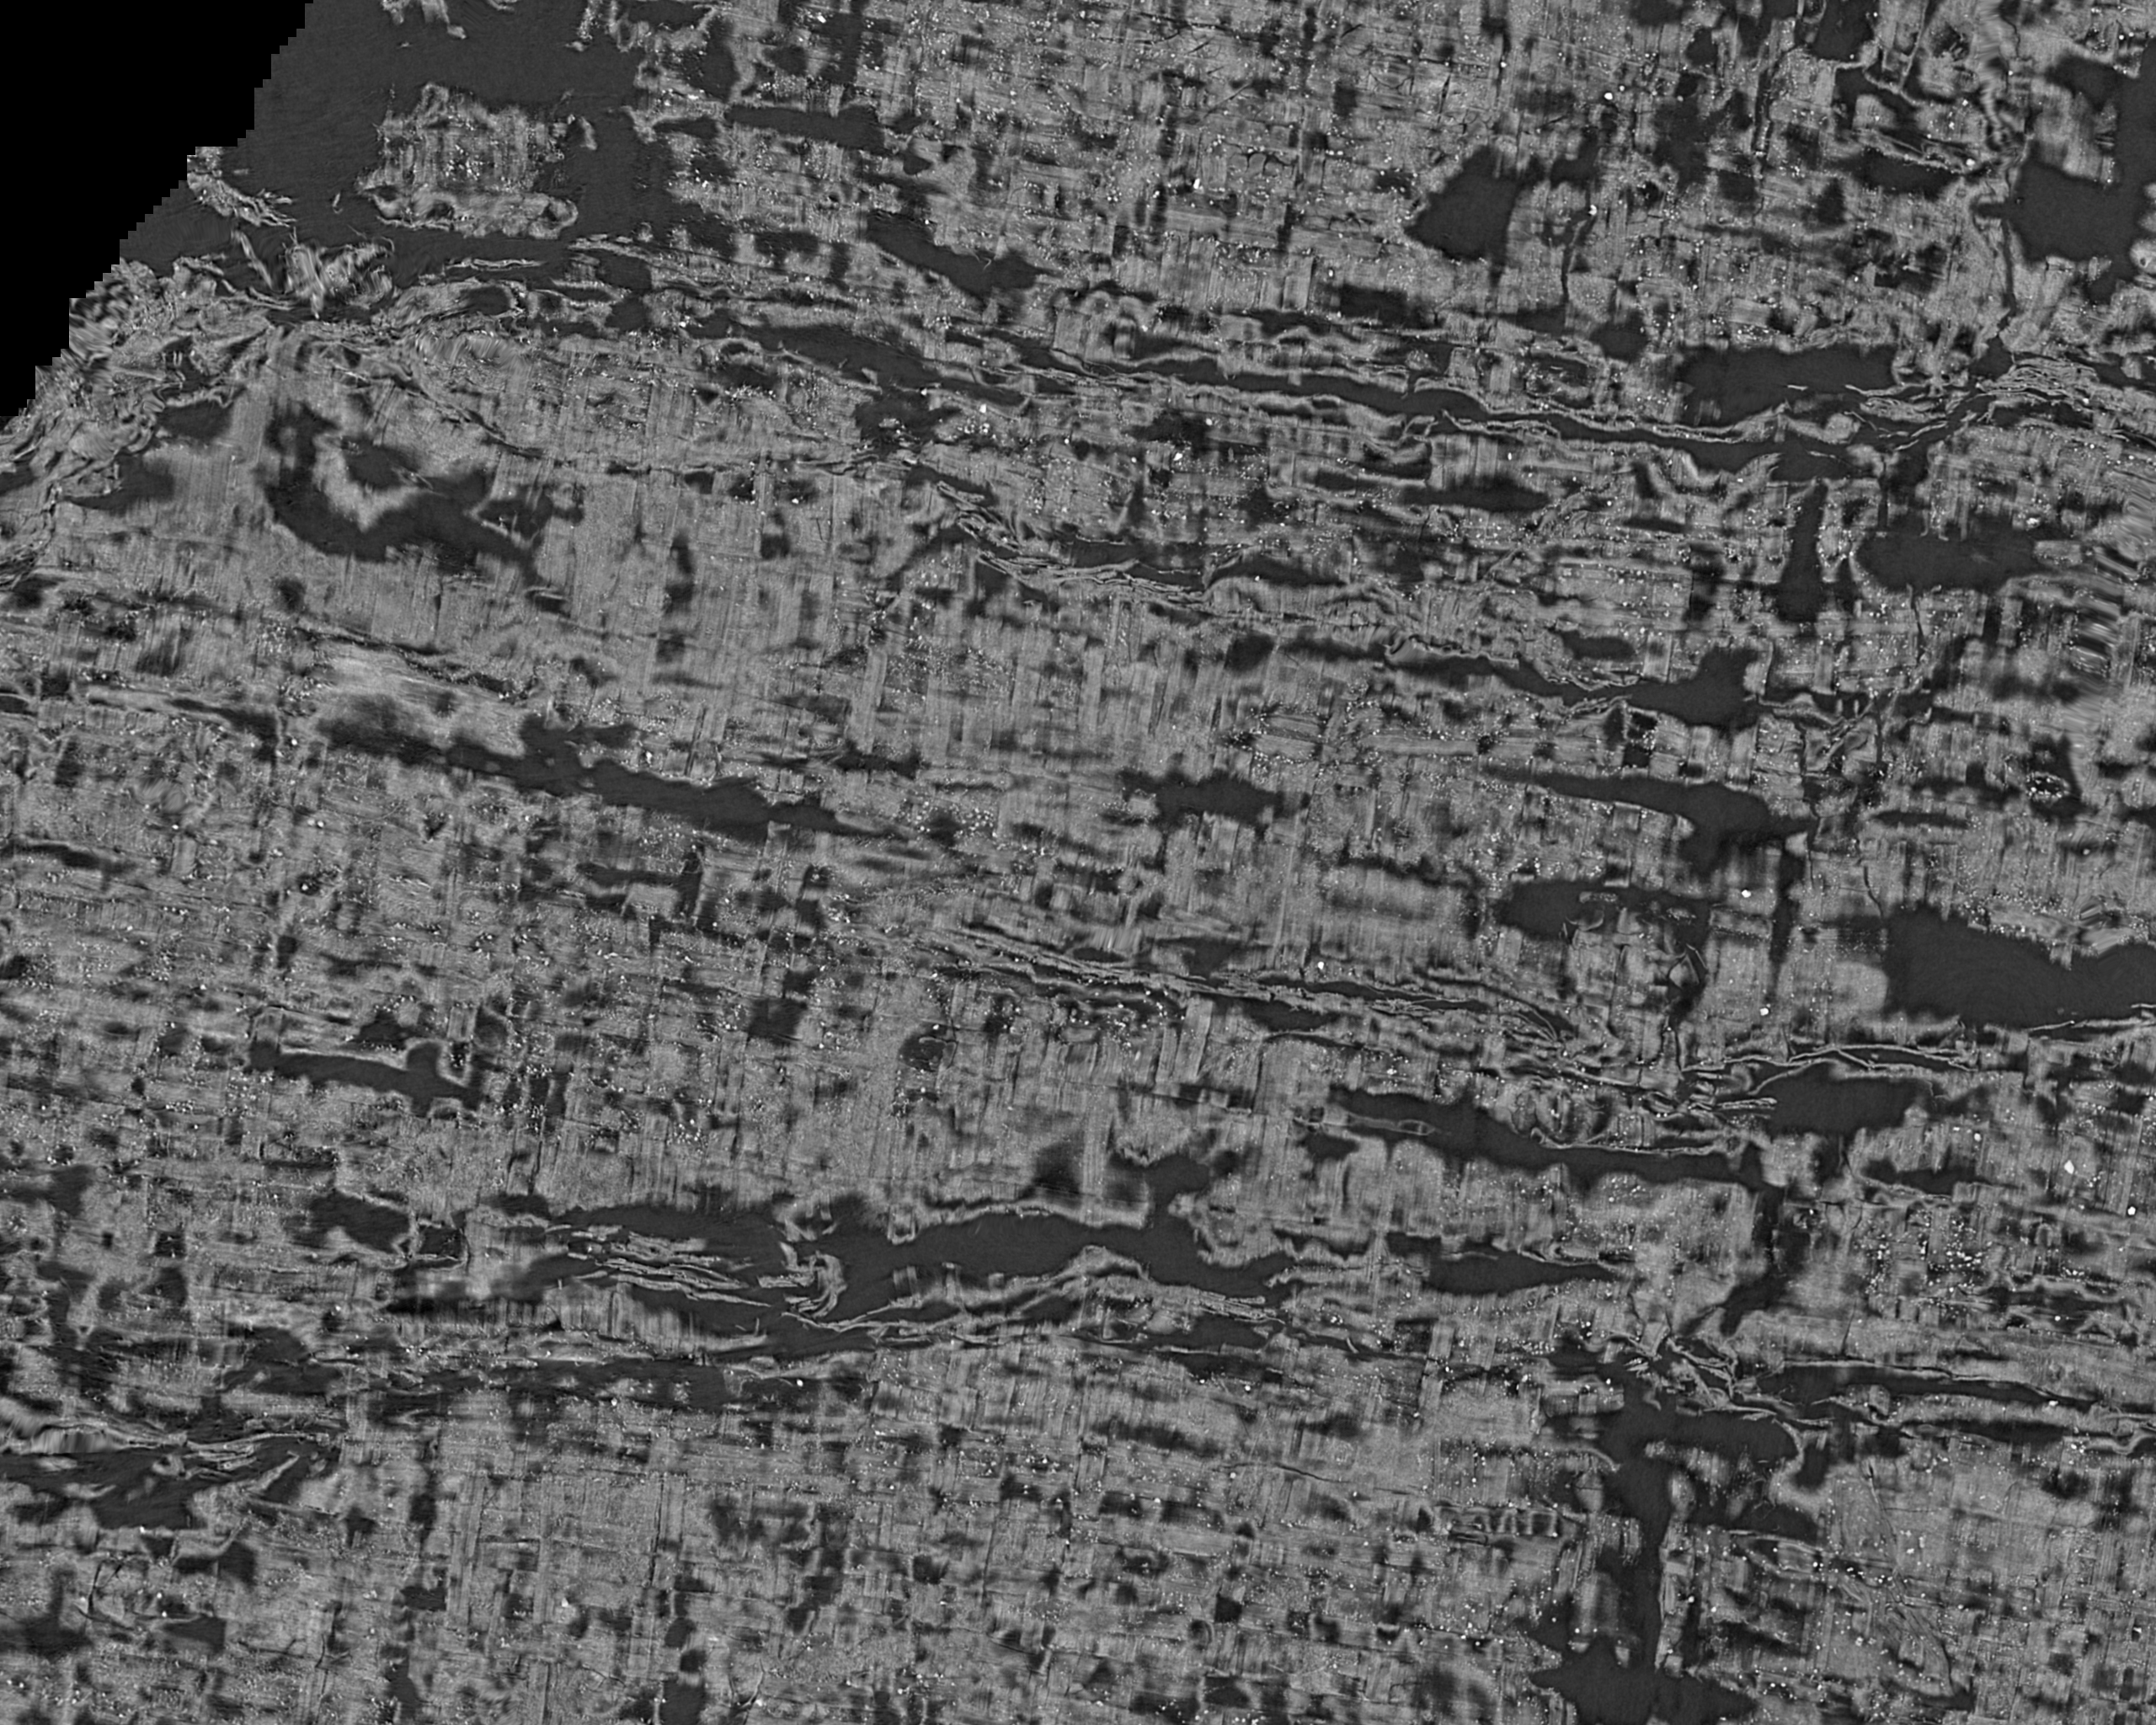
\includegraphics[width=122.48pt]{../figures/ag1/ag1_1_texture.png}}\end{minipage}\hspace{2pt}\begin{minipage}[t]{122.48pt}\centering\href{https://raw.githubusercontent.com/evilaliv3/vesuvius-challenge-pipeline/main/results/db27c806-rectina/src/figures/ag1/ag1_2_labels.png}{
\includegraphics[width=122.48pt]{../figures/ag1/ag1_2_labels.png}}\end{minipage}}
\par\vspace{4pt}
\noindent\makebox[\columnwidth][c]{\begin{minipage}[t]{122.48pt}\centering\href{https://raw.githubusercontent.com/evilaliv3/vesuvius-challenge-pipeline/main/results/db27c806-rectina/src/figures/ag1/ag1_3_reader-v2.png}{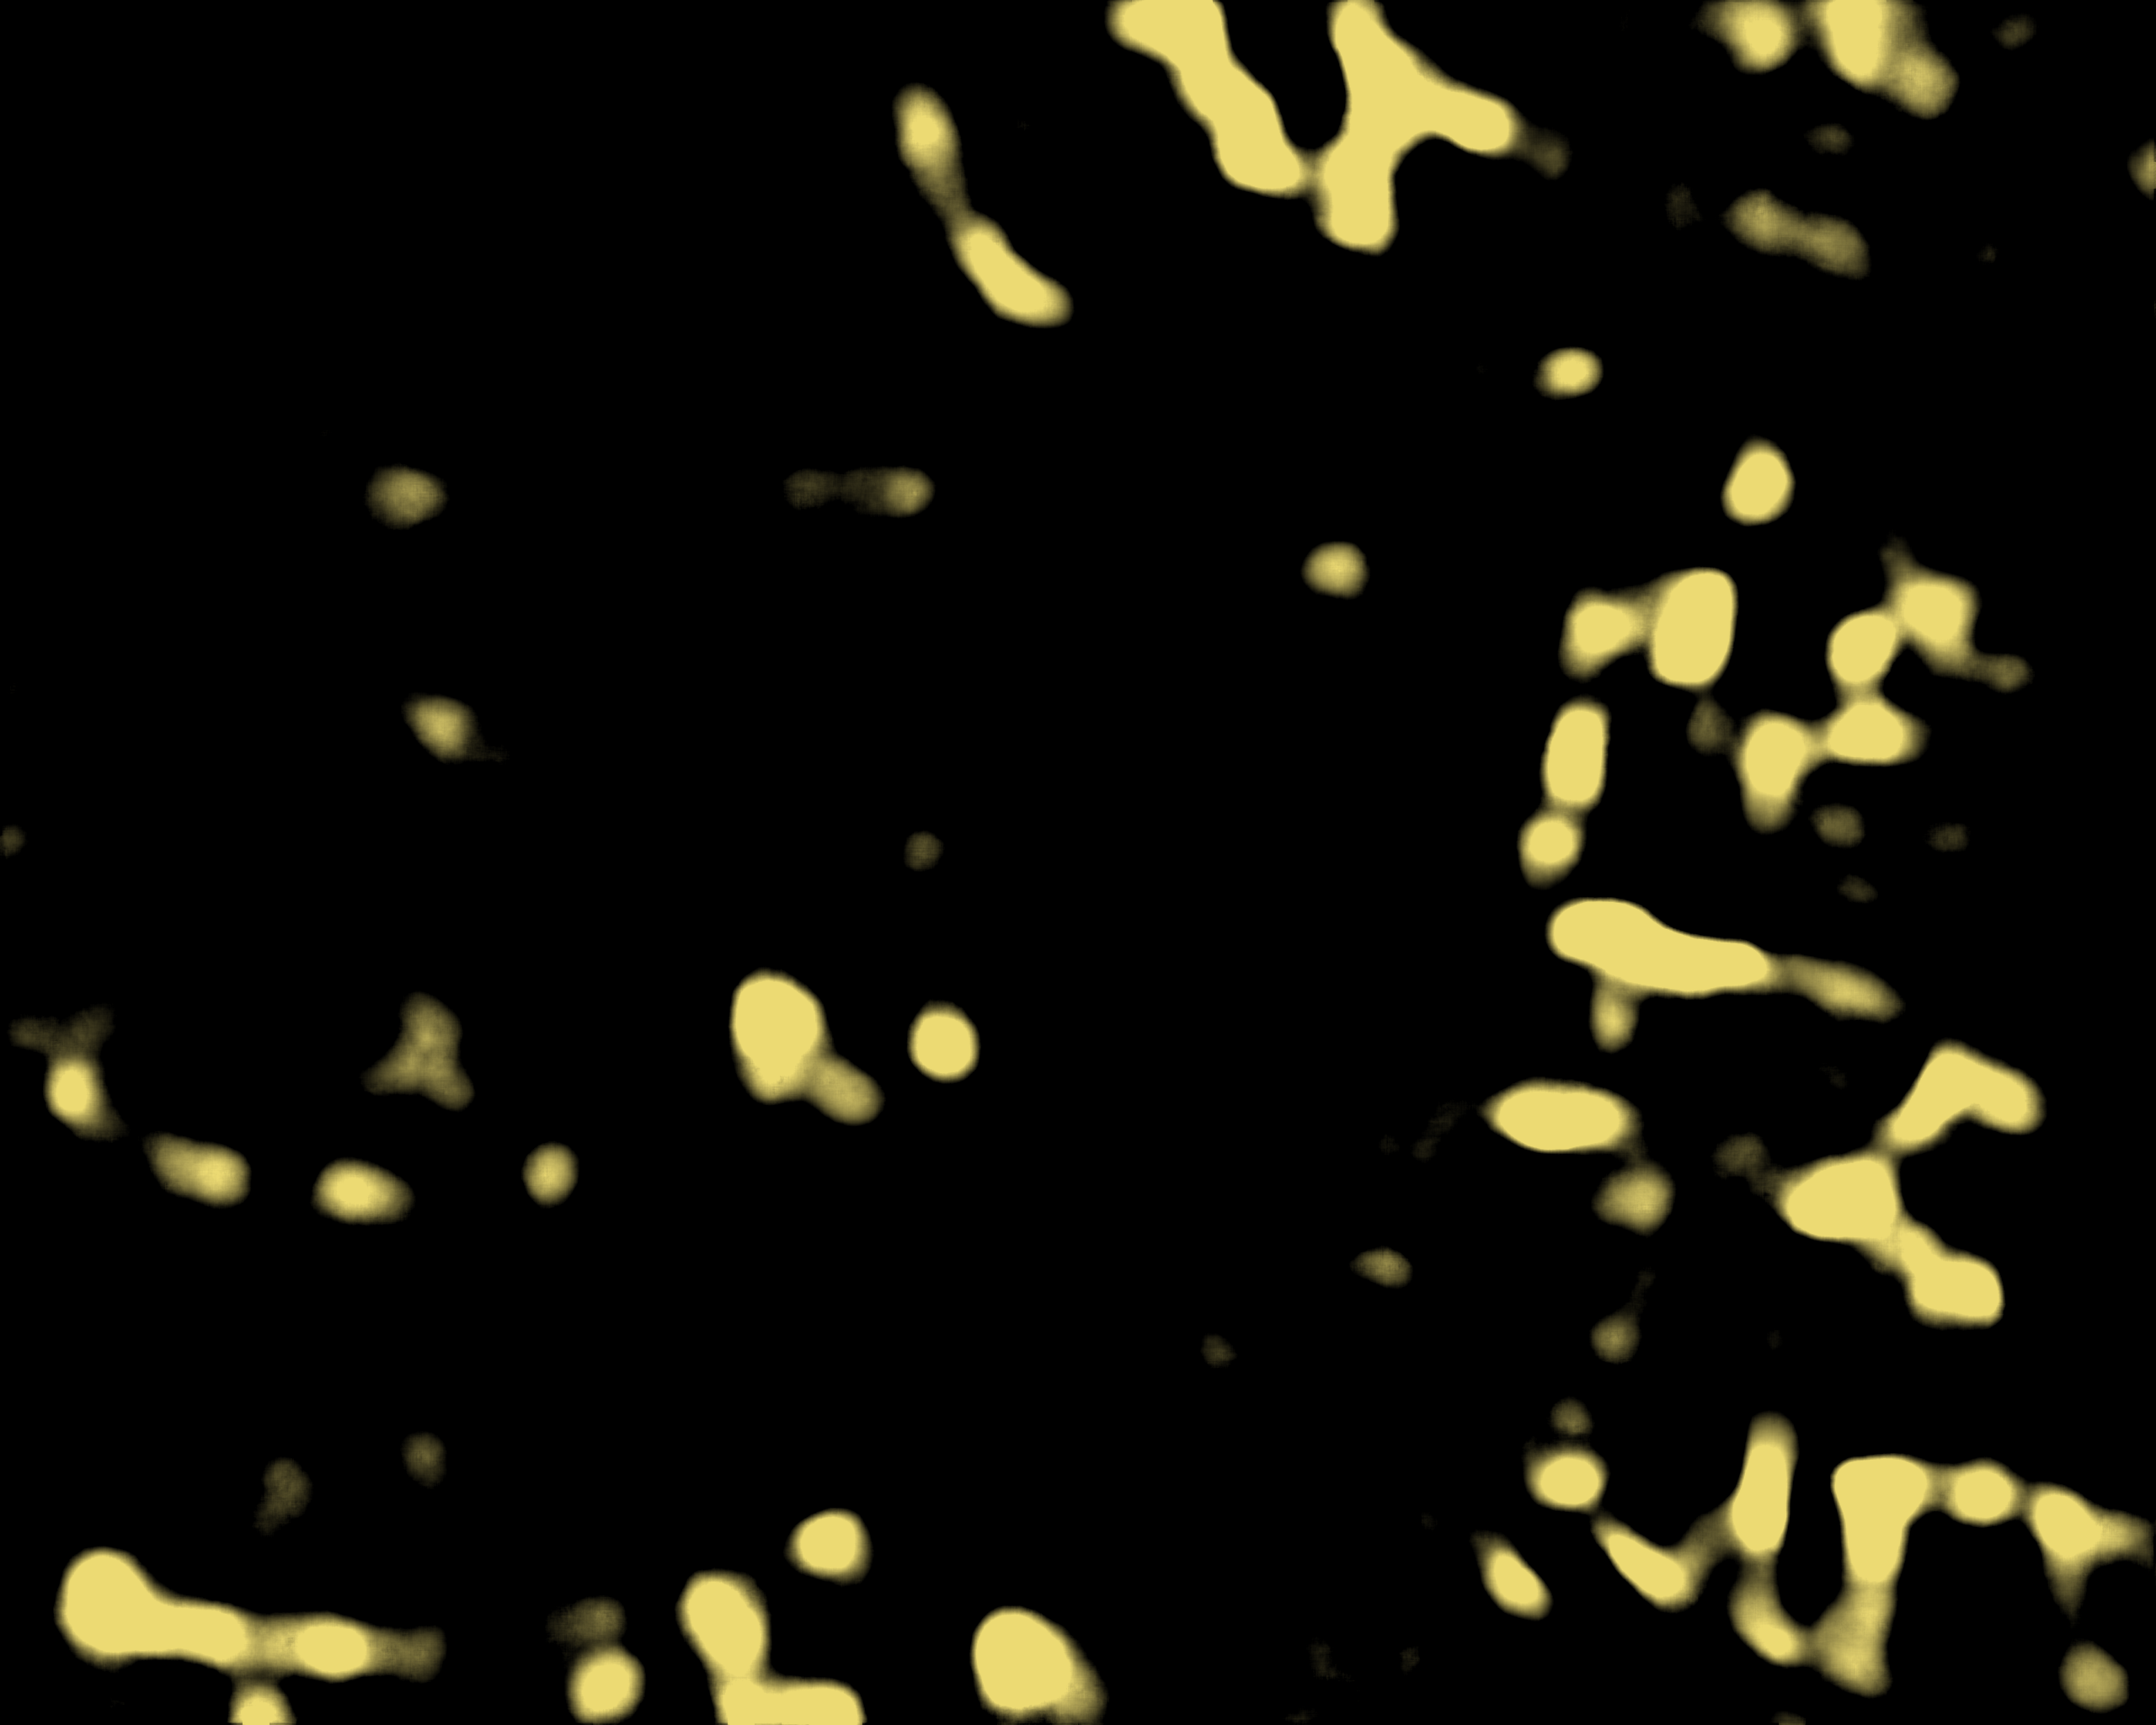
\includegraphics[width=122.48pt]{../figures/ag1/ag1_3_reader-v2.png}}\end{minipage}\hspace{2pt}\begin{minipage}[t]{122.48pt}\centering\href{https://raw.githubusercontent.com/evilaliv3/vesuvius-challenge-pipeline/main/results/db27c806-rectina/src/figures/ag1/ag1_5_rectina-m1.png}{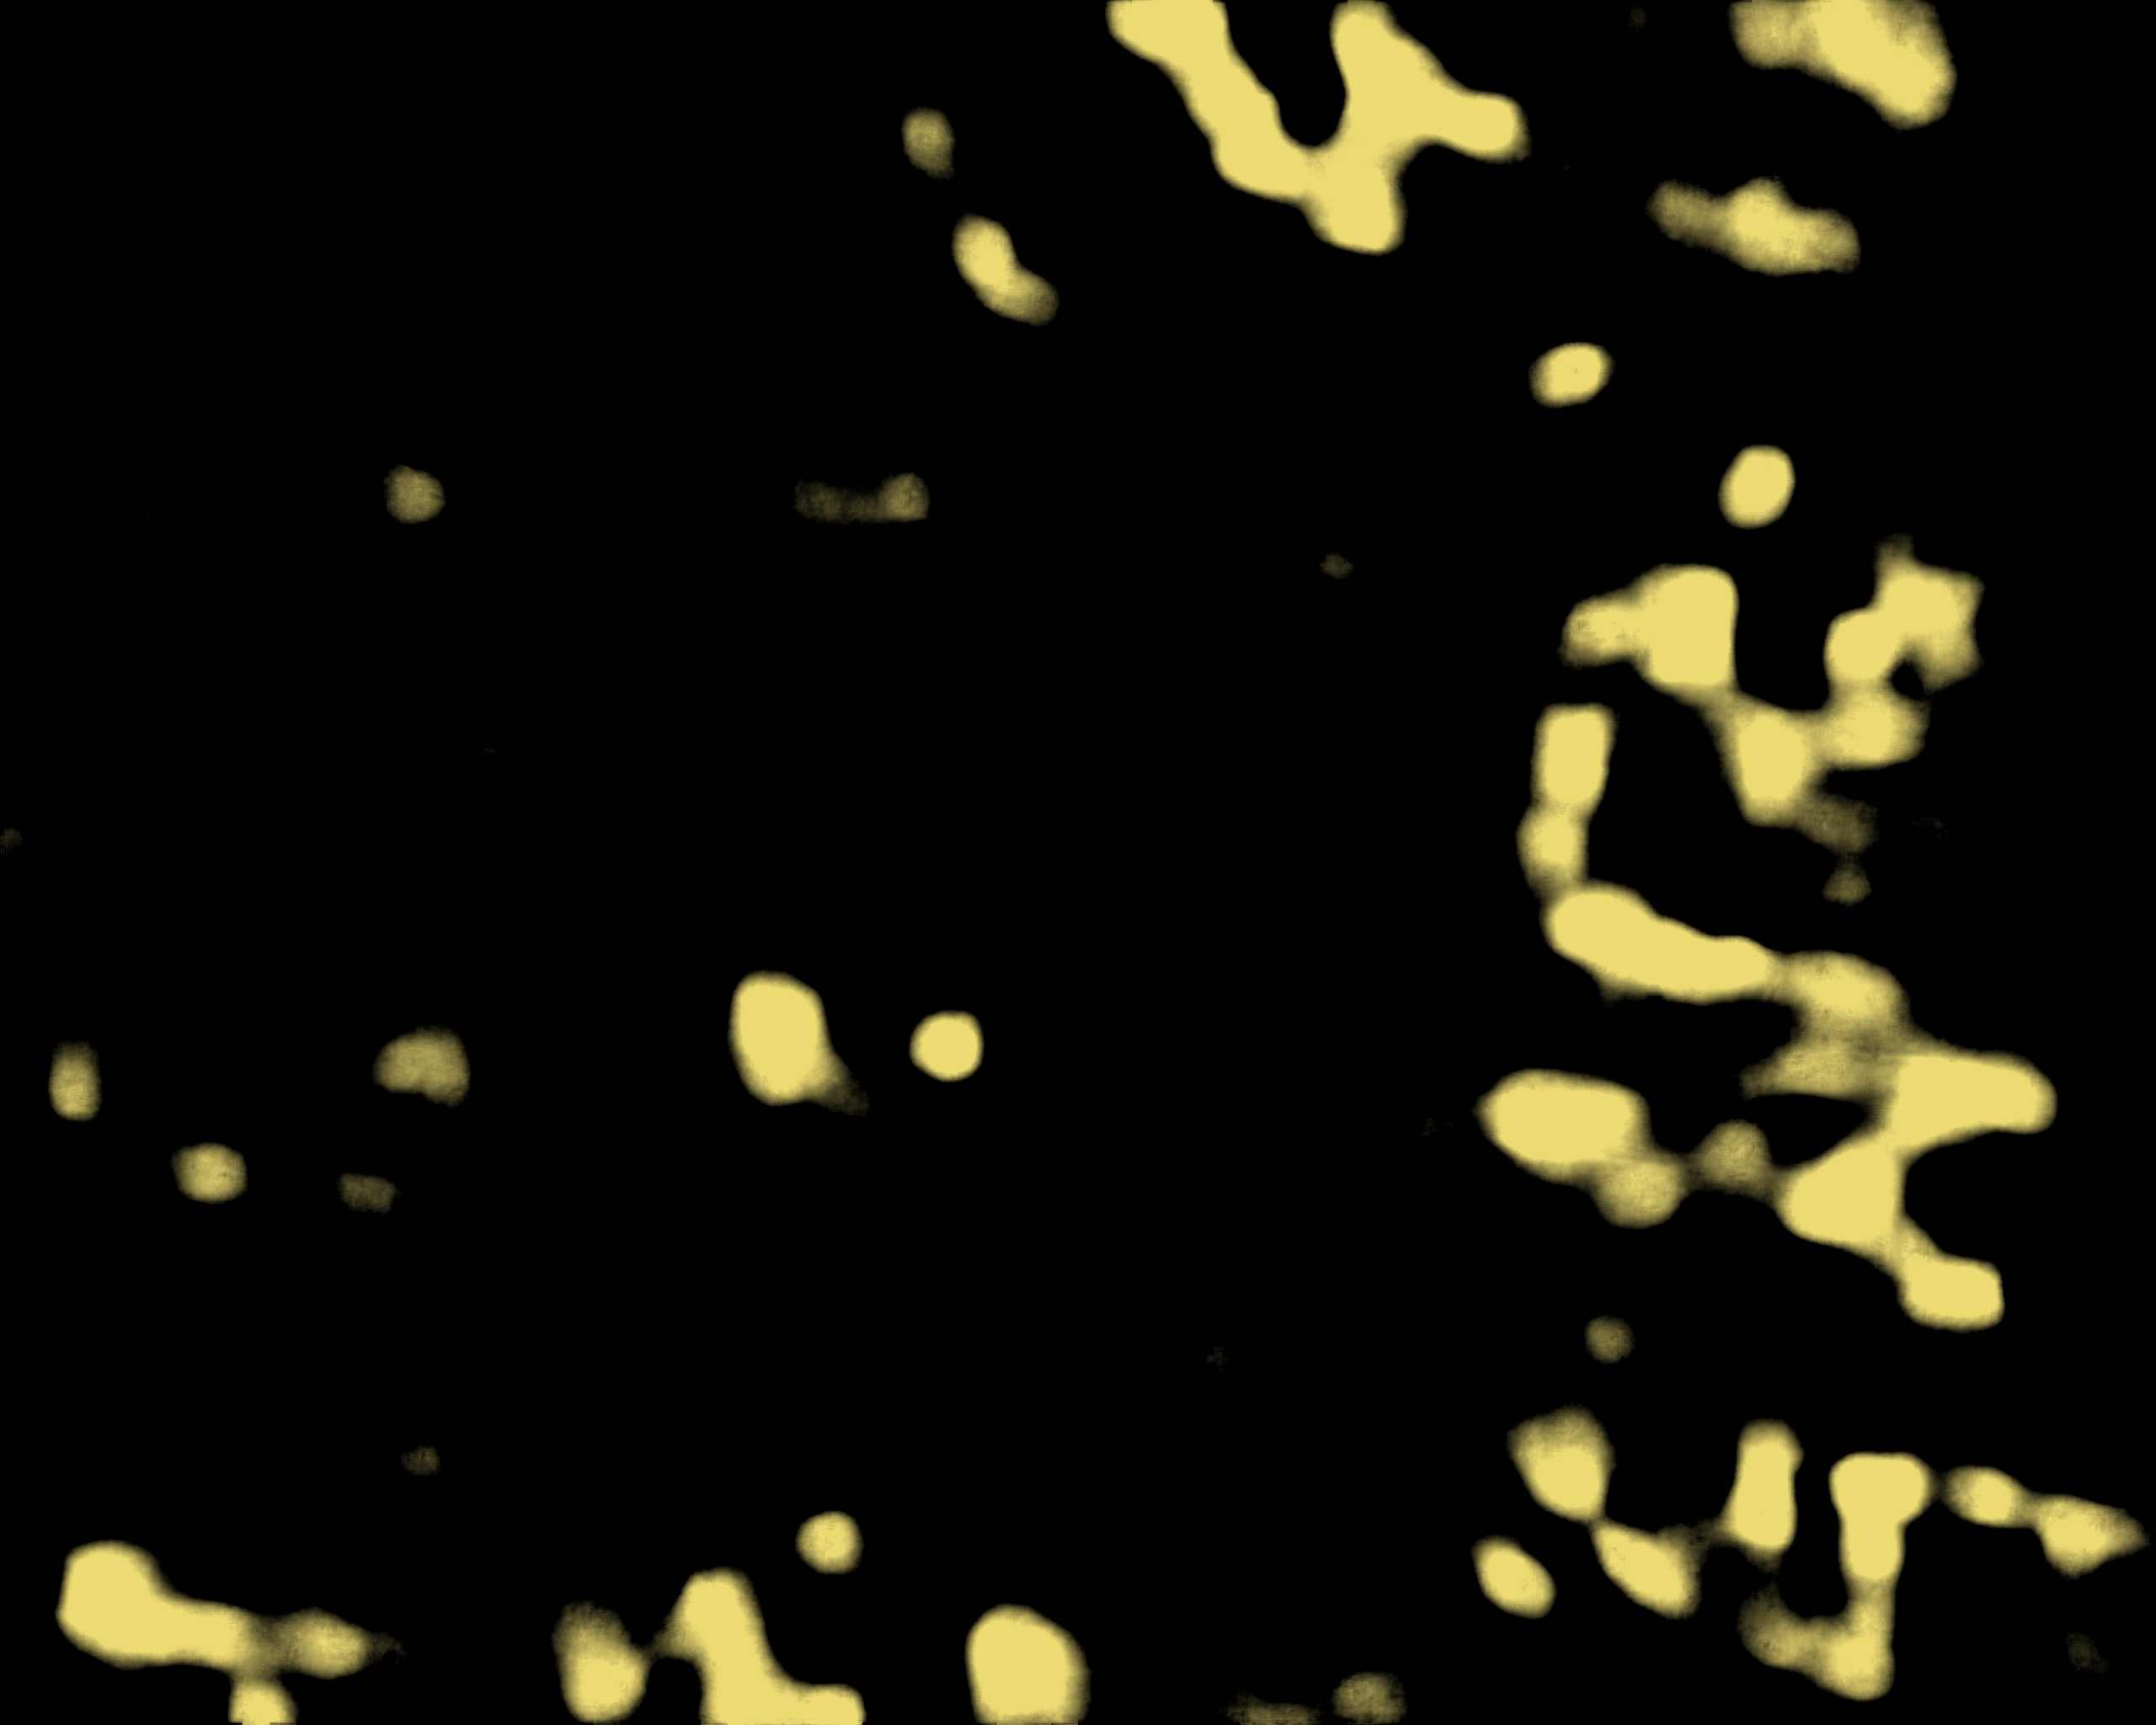
\includegraphics[width=122.48pt]{../figures/ag1/ag1_5_rectina-m1.png}}\end{minipage}}
\par\vspace{4pt}
\noindent\makebox[\columnwidth][c]{\begin{minipage}[t]{122.48pt}\centering\href{https://raw.githubusercontent.com/evilaliv3/vesuvius-challenge-pipeline/main/results/db27c806-rectina/src/figures/ag1/ag1_4_reader-v3.png}{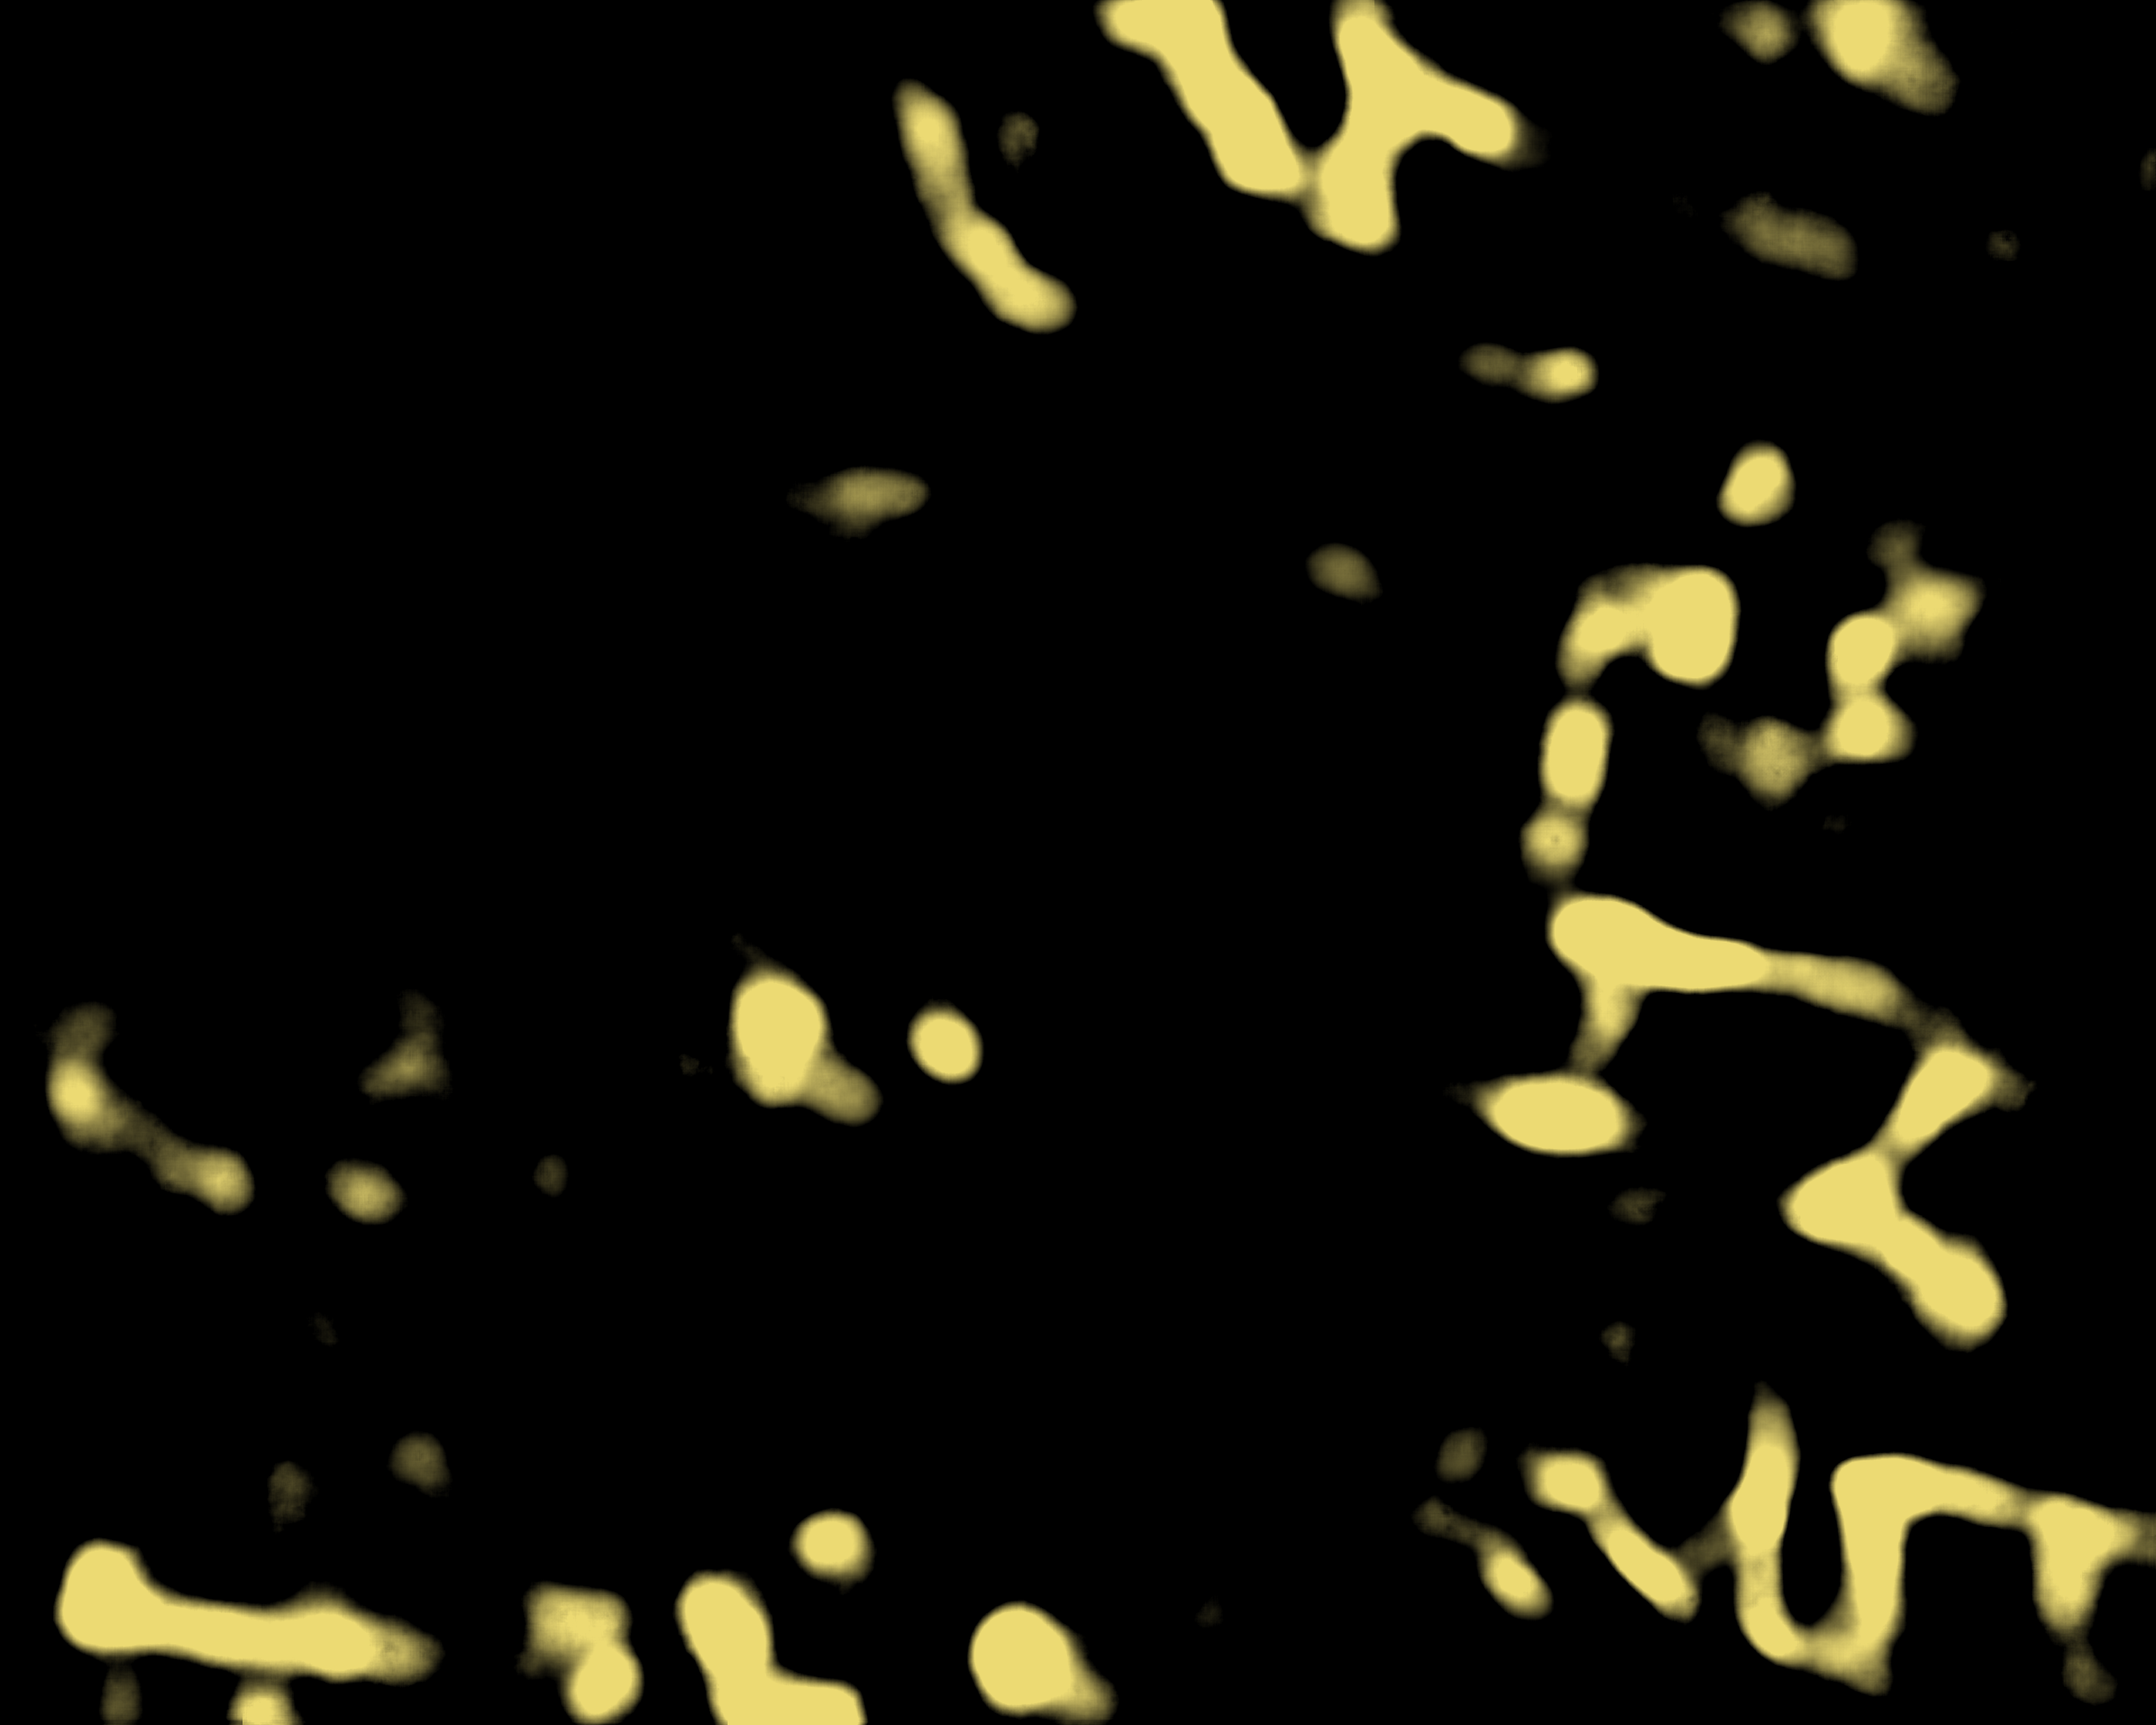
\includegraphics[width=122.48pt]{../figures/ag1/ag1_4_reader-v3.png}}\end{minipage}\hspace{2pt}\begin{minipage}[t]{122.48pt}\centering\href{https://raw.githubusercontent.com/evilaliv3/vesuvius-challenge-pipeline/main/results/db27c806-rectina/src/figures/ag1/ag1_6_rectina-m2.png}{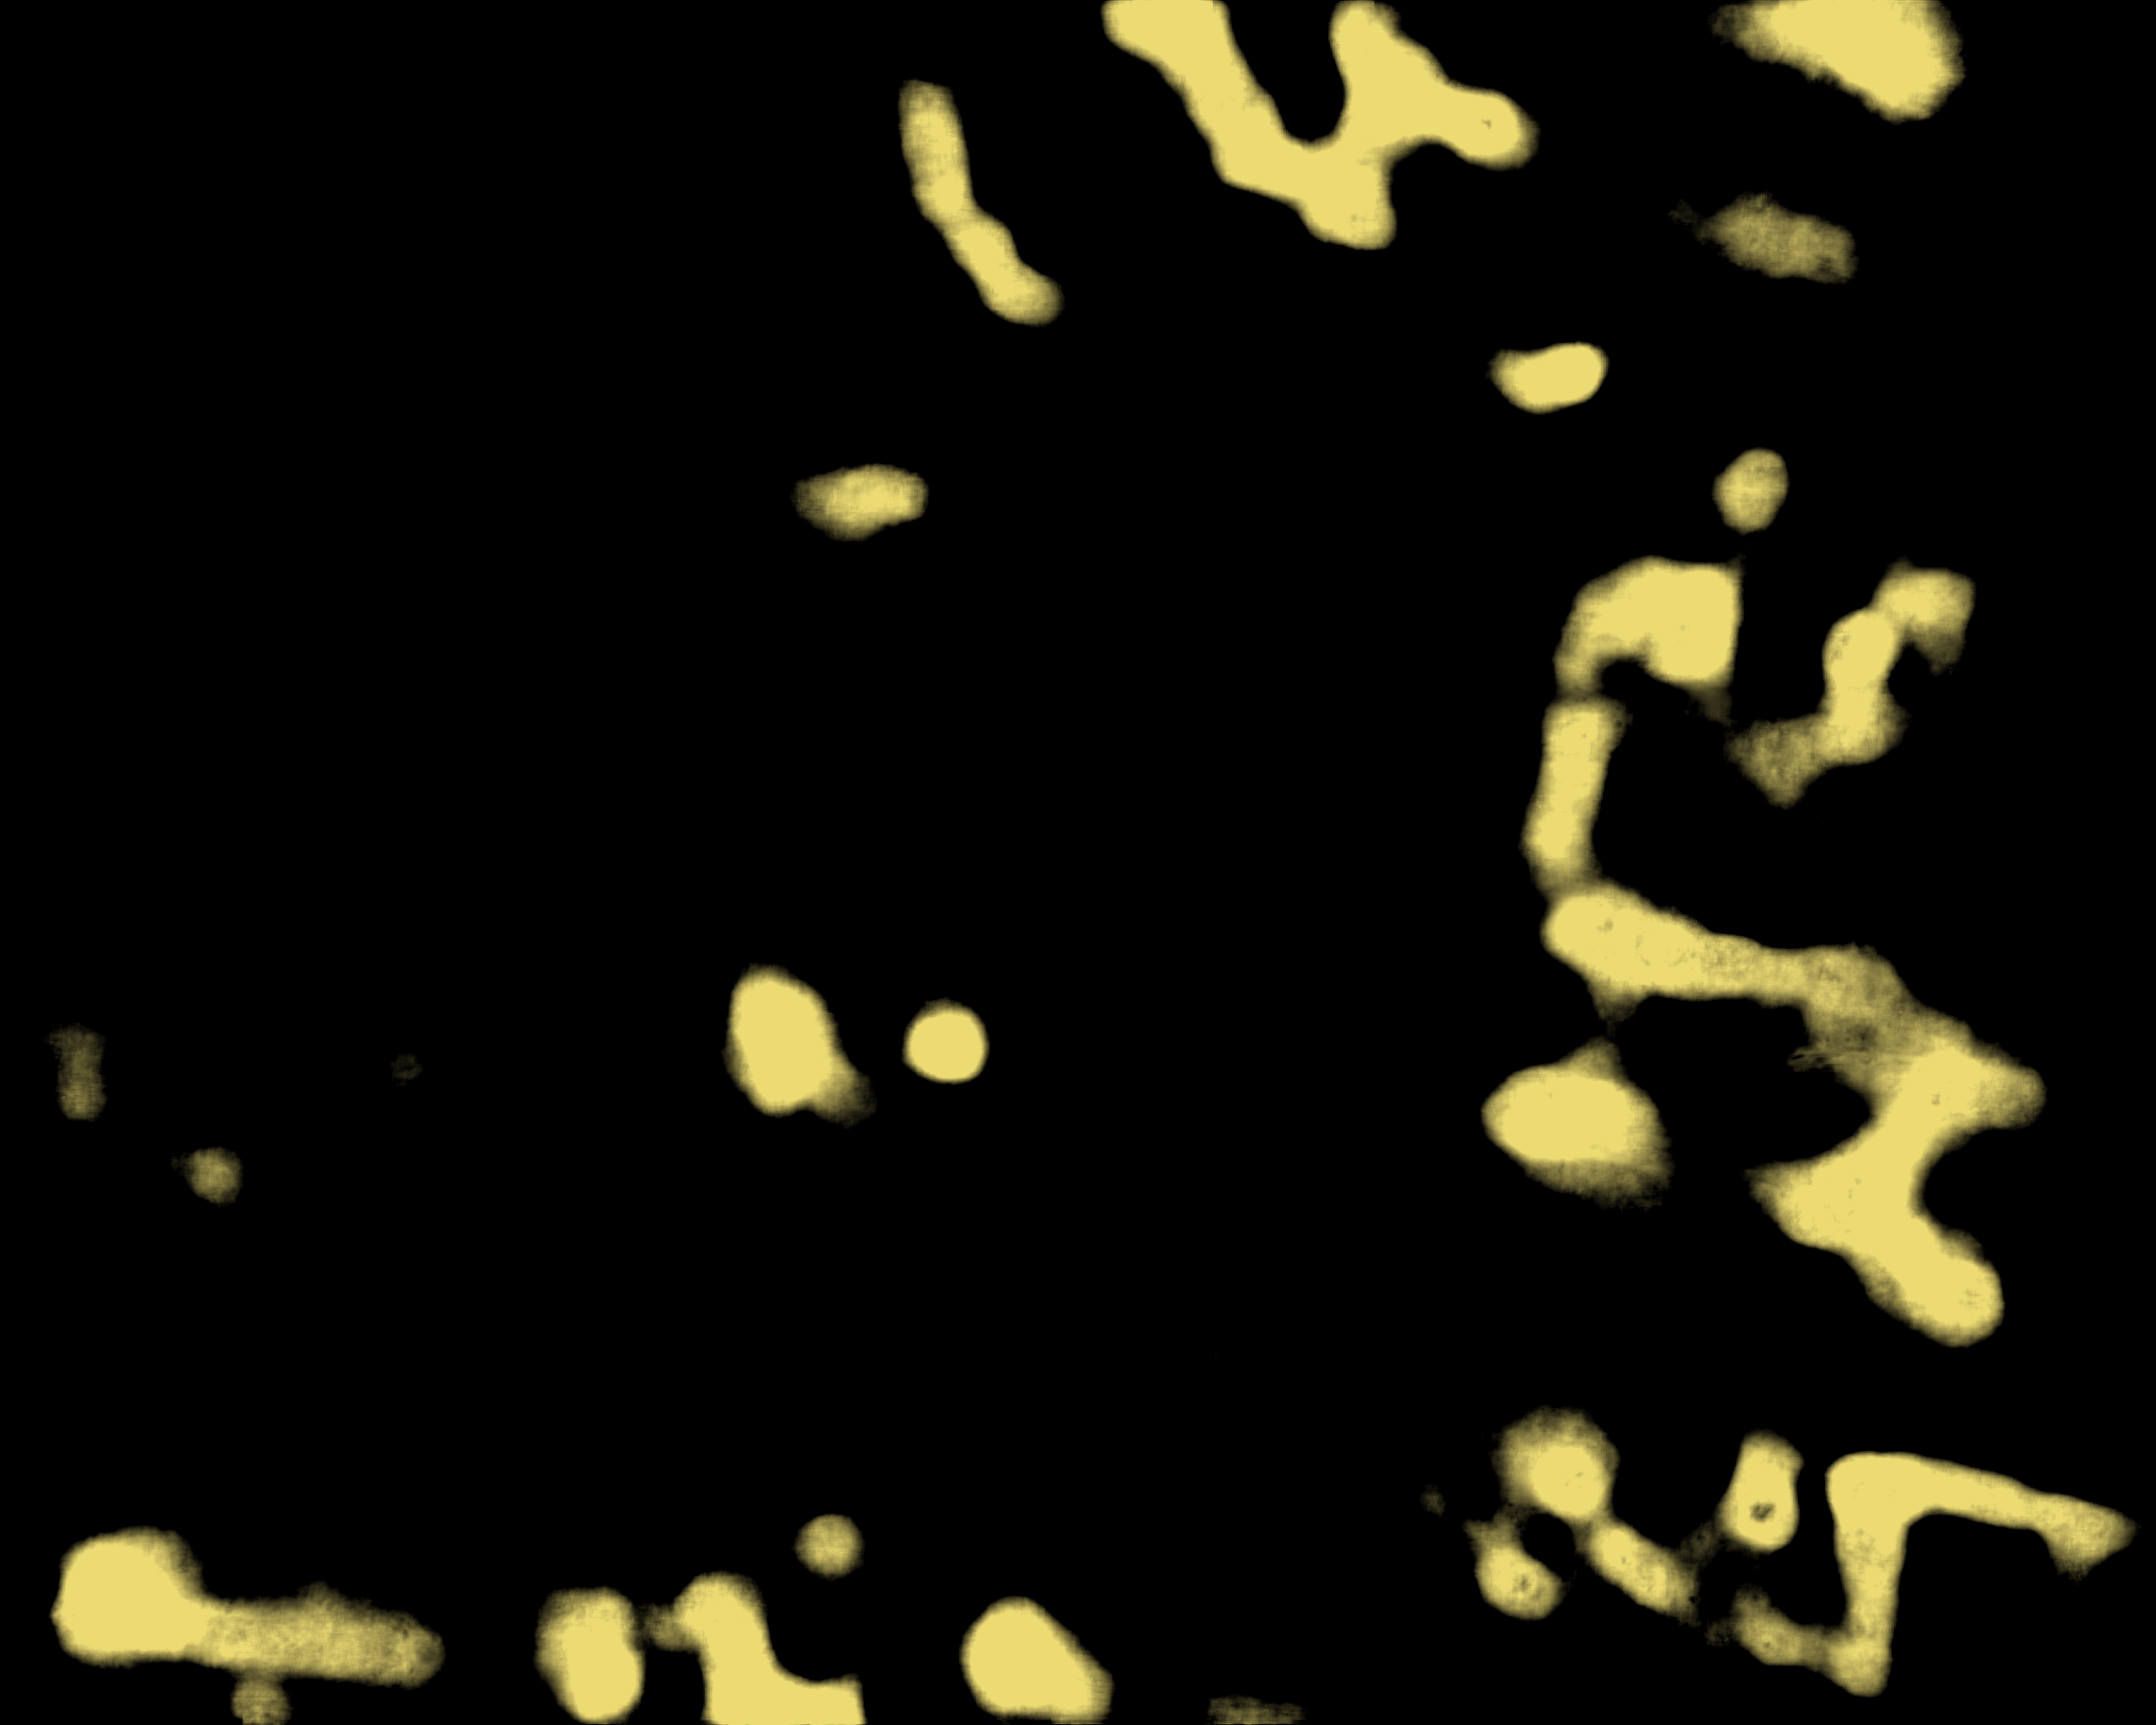
\includegraphics[width=122.48pt]{../figures/ag1/ag1_6_rectina-m2.png}}\end{minipage}}
\caption{Control unit 0841 ag1, three rows of two panels. Row 1: left, Texture; right, Labels. Row 2: left, Reader v2; right, Rectina m1 (display windows: Reader v2 0.447222 to 0.621051 (ramp); Rectina m1 0.623262 to 0.741702 (ramp)). Row 3: left, Reader v3; right, Rectina m2 (display windows: Reader v3 0.470294 to 0.693186 (ramp); Rectina m2 0.671638 to 0.774498 (ramp)). Each map is stretched between its own percentiles. Reader and model stand side by side in the rows 2 and 3.}
\end{figure}

\begin{figure}[!tbp]
\centering
\noindent\makebox[\columnwidth][c]{\begin{minipage}[t]{122.48pt}\centering\href{https://raw.githubusercontent.com/evilaliv3/vesuvius-challenge-pipeline/main/results/db27c806-rectina/src/figures/ag2/ag2_1_texture.png}{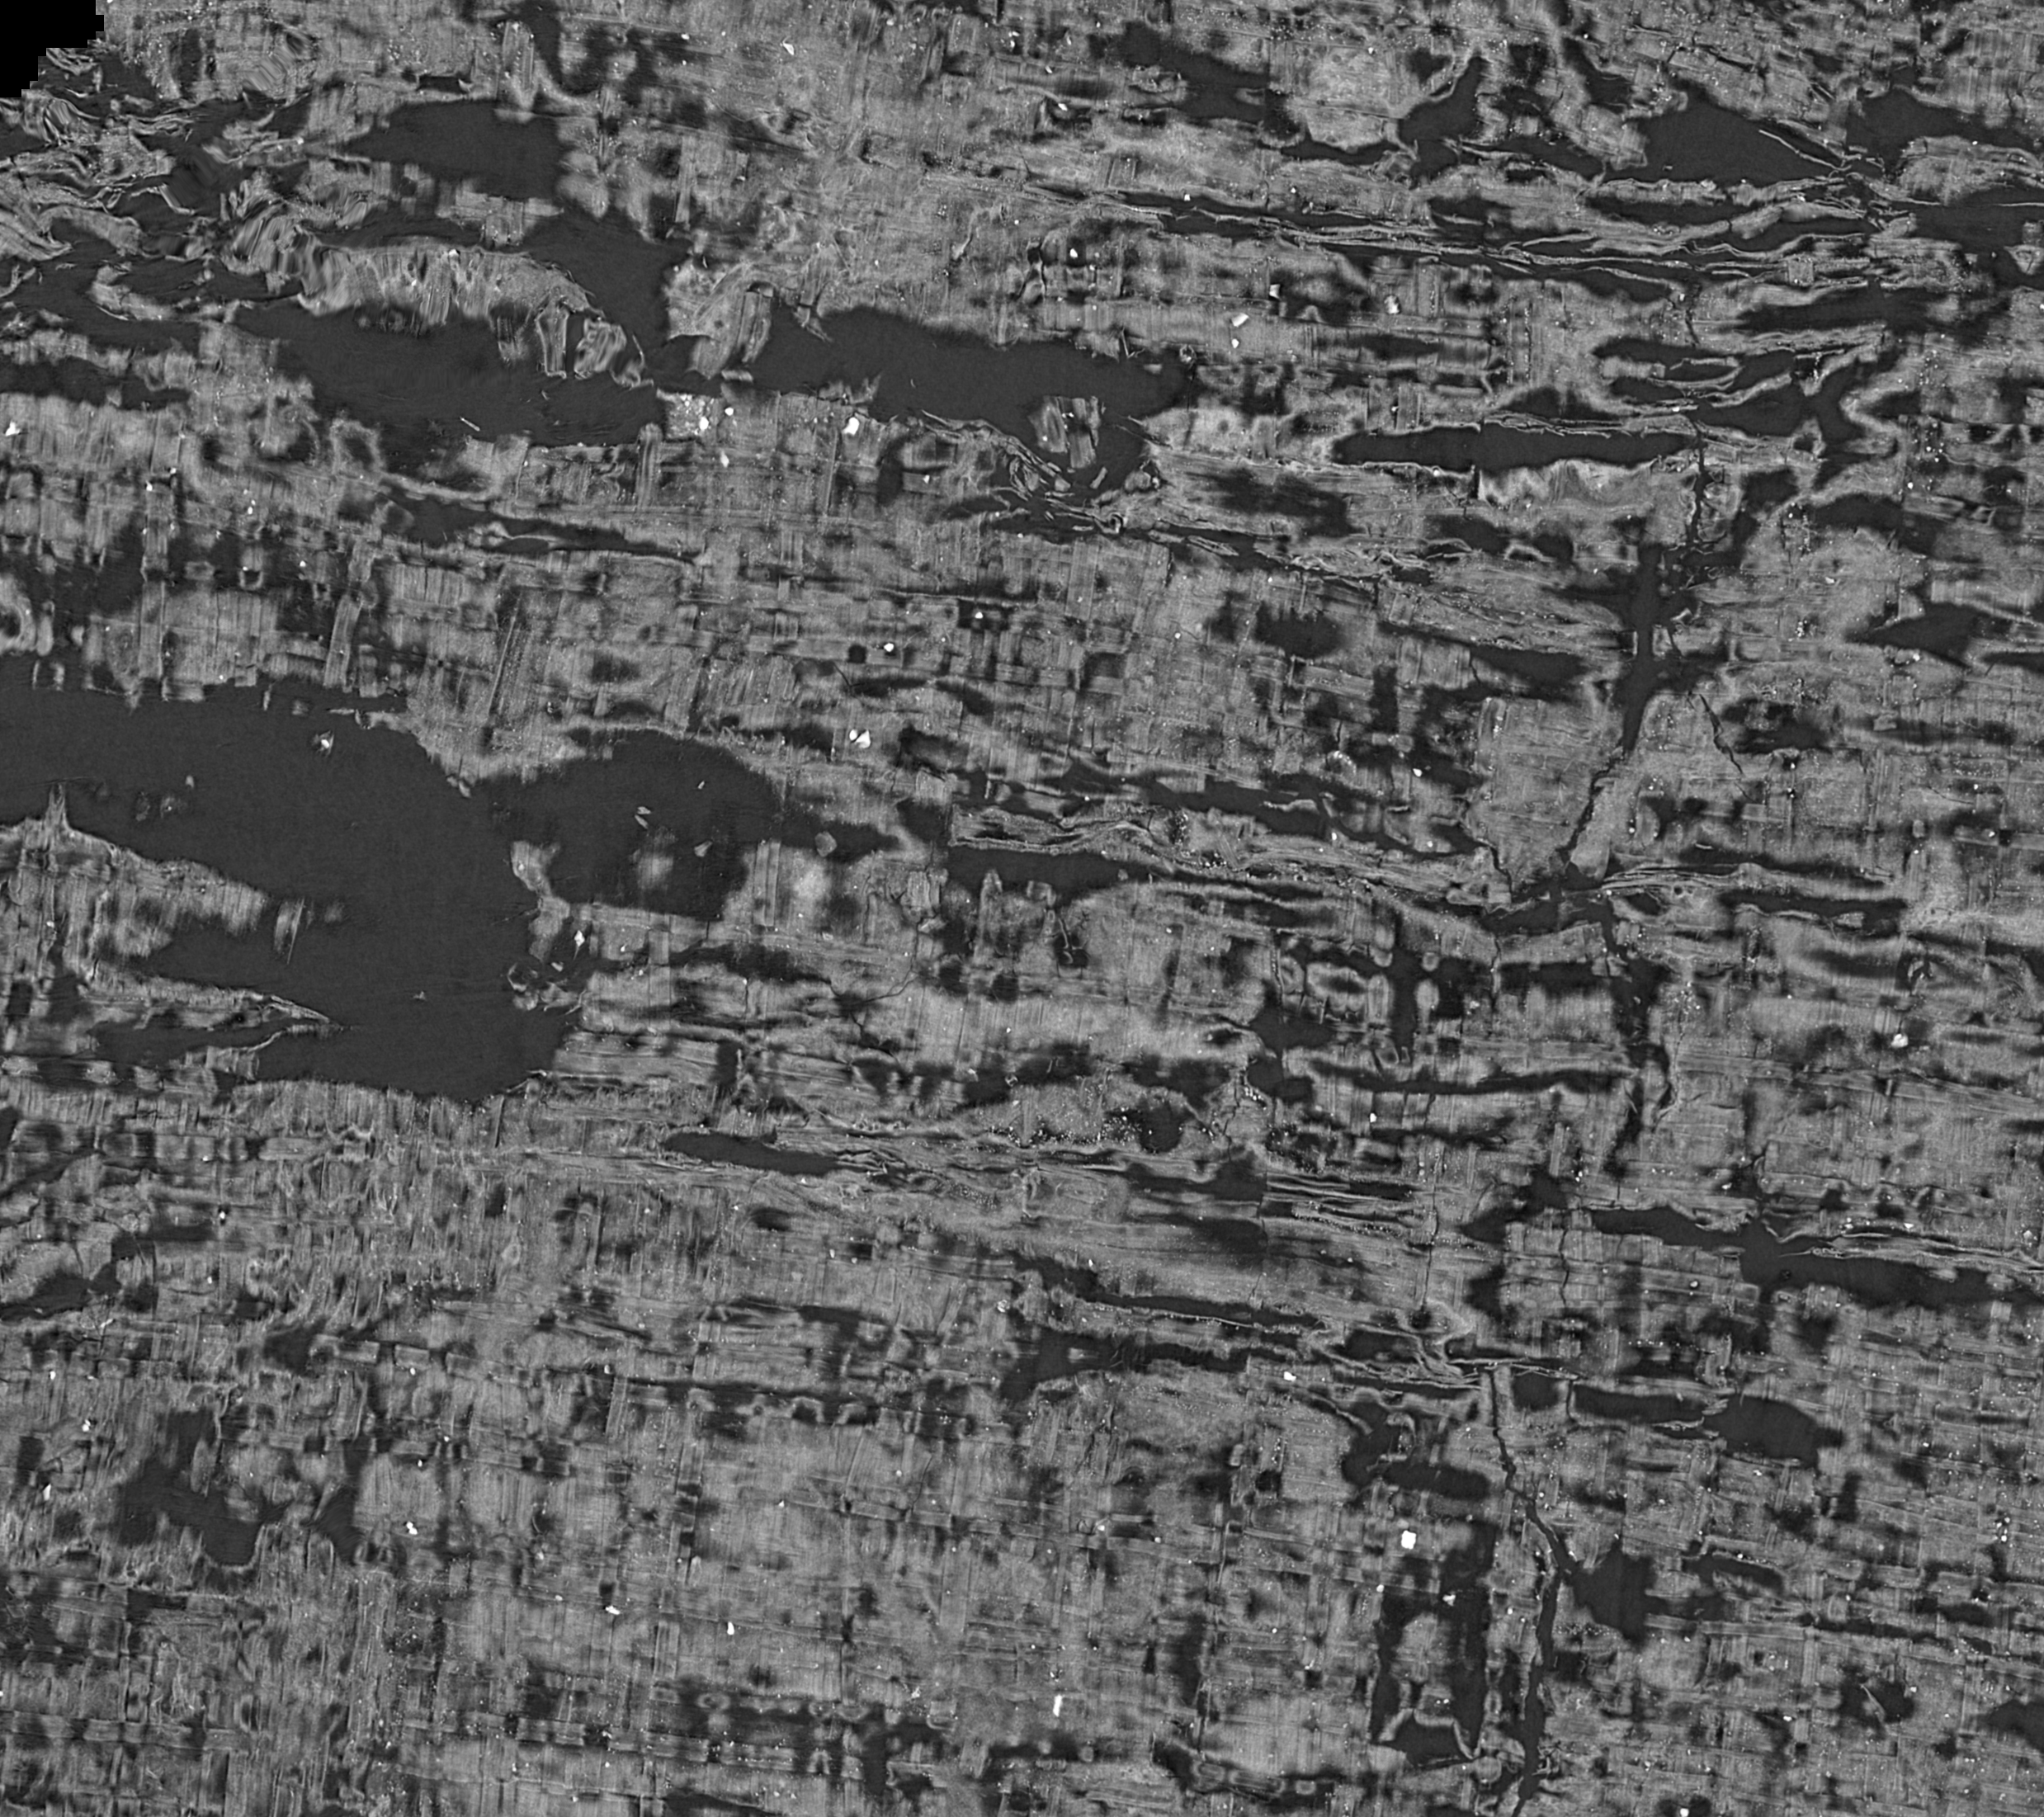
\includegraphics[width=122.48pt]{../figures/ag2/ag2_1_texture.png}}\end{minipage}\hspace{2pt}\begin{minipage}[t]{122.48pt}\centering\href{https://raw.githubusercontent.com/evilaliv3/vesuvius-challenge-pipeline/main/results/db27c806-rectina/src/figures/ag2/ag2_2_labels.png}{
\includegraphics[width=122.48pt]{../figures/ag2/ag2_2_labels.png}}\end{minipage}}
\par\vspace{4pt}
\noindent\makebox[\columnwidth][c]{\begin{minipage}[t]{122.48pt}\centering\href{https://raw.githubusercontent.com/evilaliv3/vesuvius-challenge-pipeline/main/results/db27c806-rectina/src/figures/ag2/ag2_3_reader-v2.png}{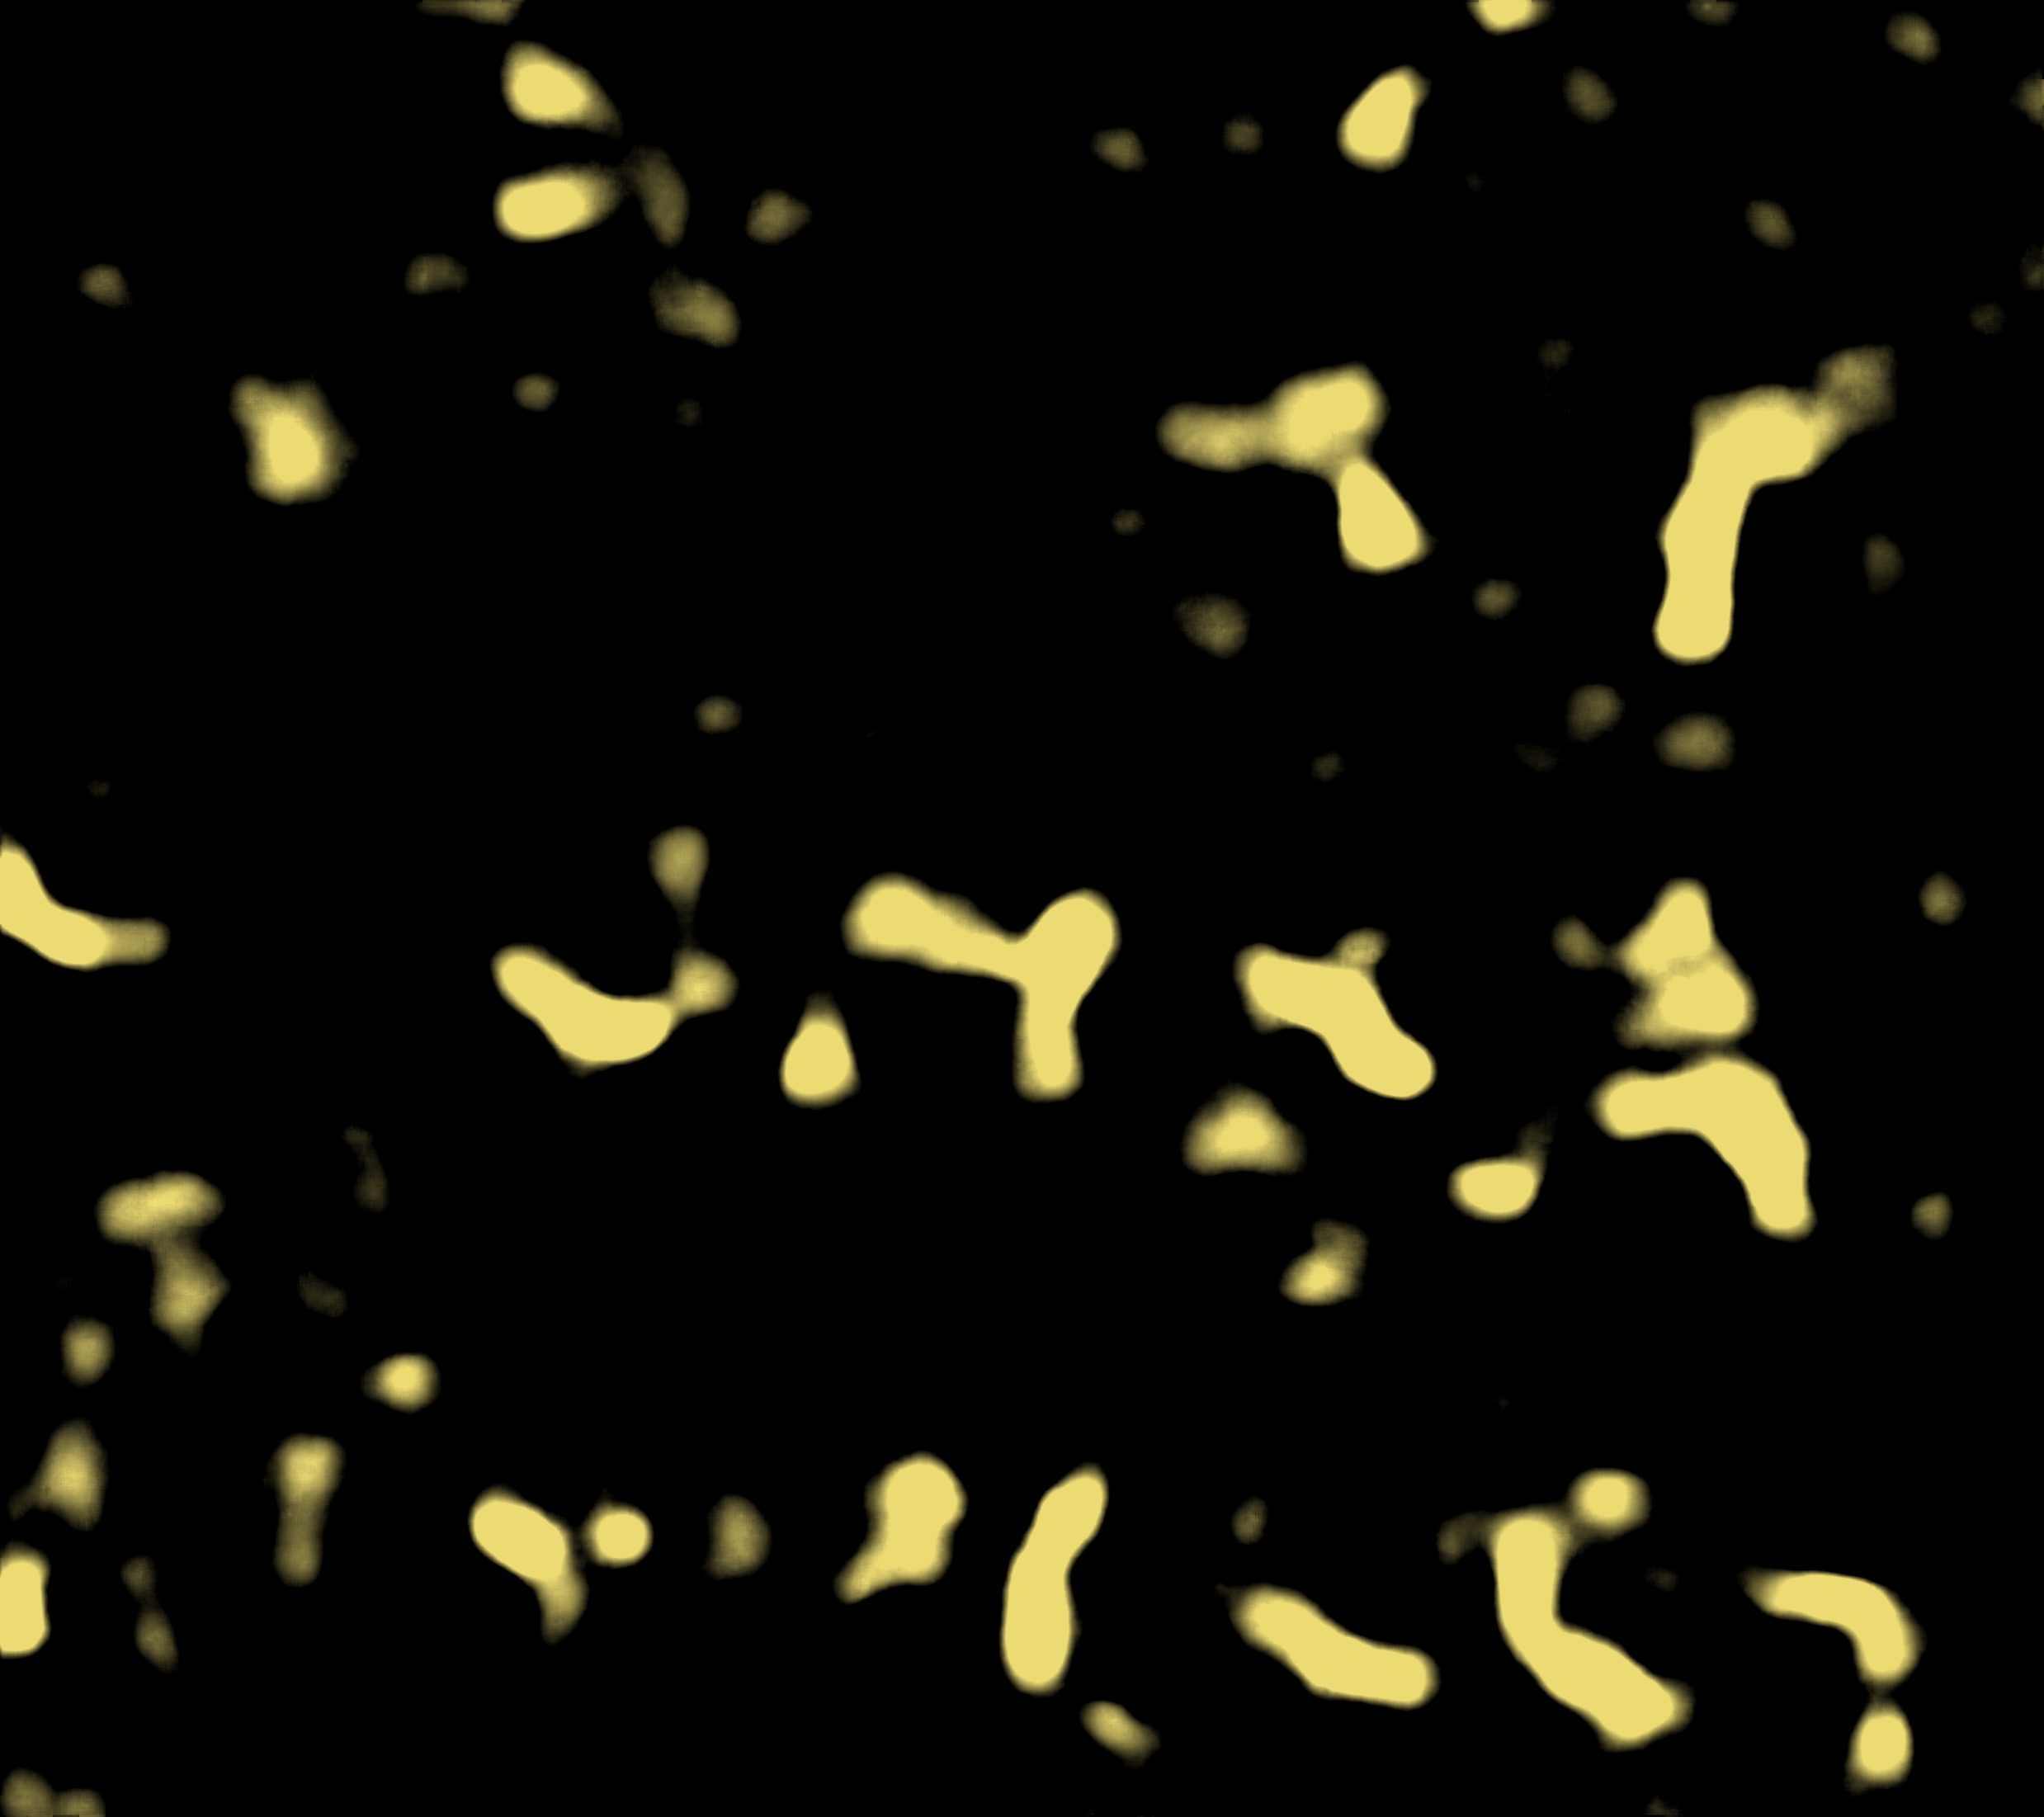
\includegraphics[width=122.48pt]{../figures/ag2/ag2_3_reader-v2.png}}\end{minipage}\hspace{2pt}\begin{minipage}[t]{122.48pt}\centering\href{https://raw.githubusercontent.com/evilaliv3/vesuvius-challenge-pipeline/main/results/db27c806-rectina/src/figures/ag2/ag2_5_rectina-m1.png}{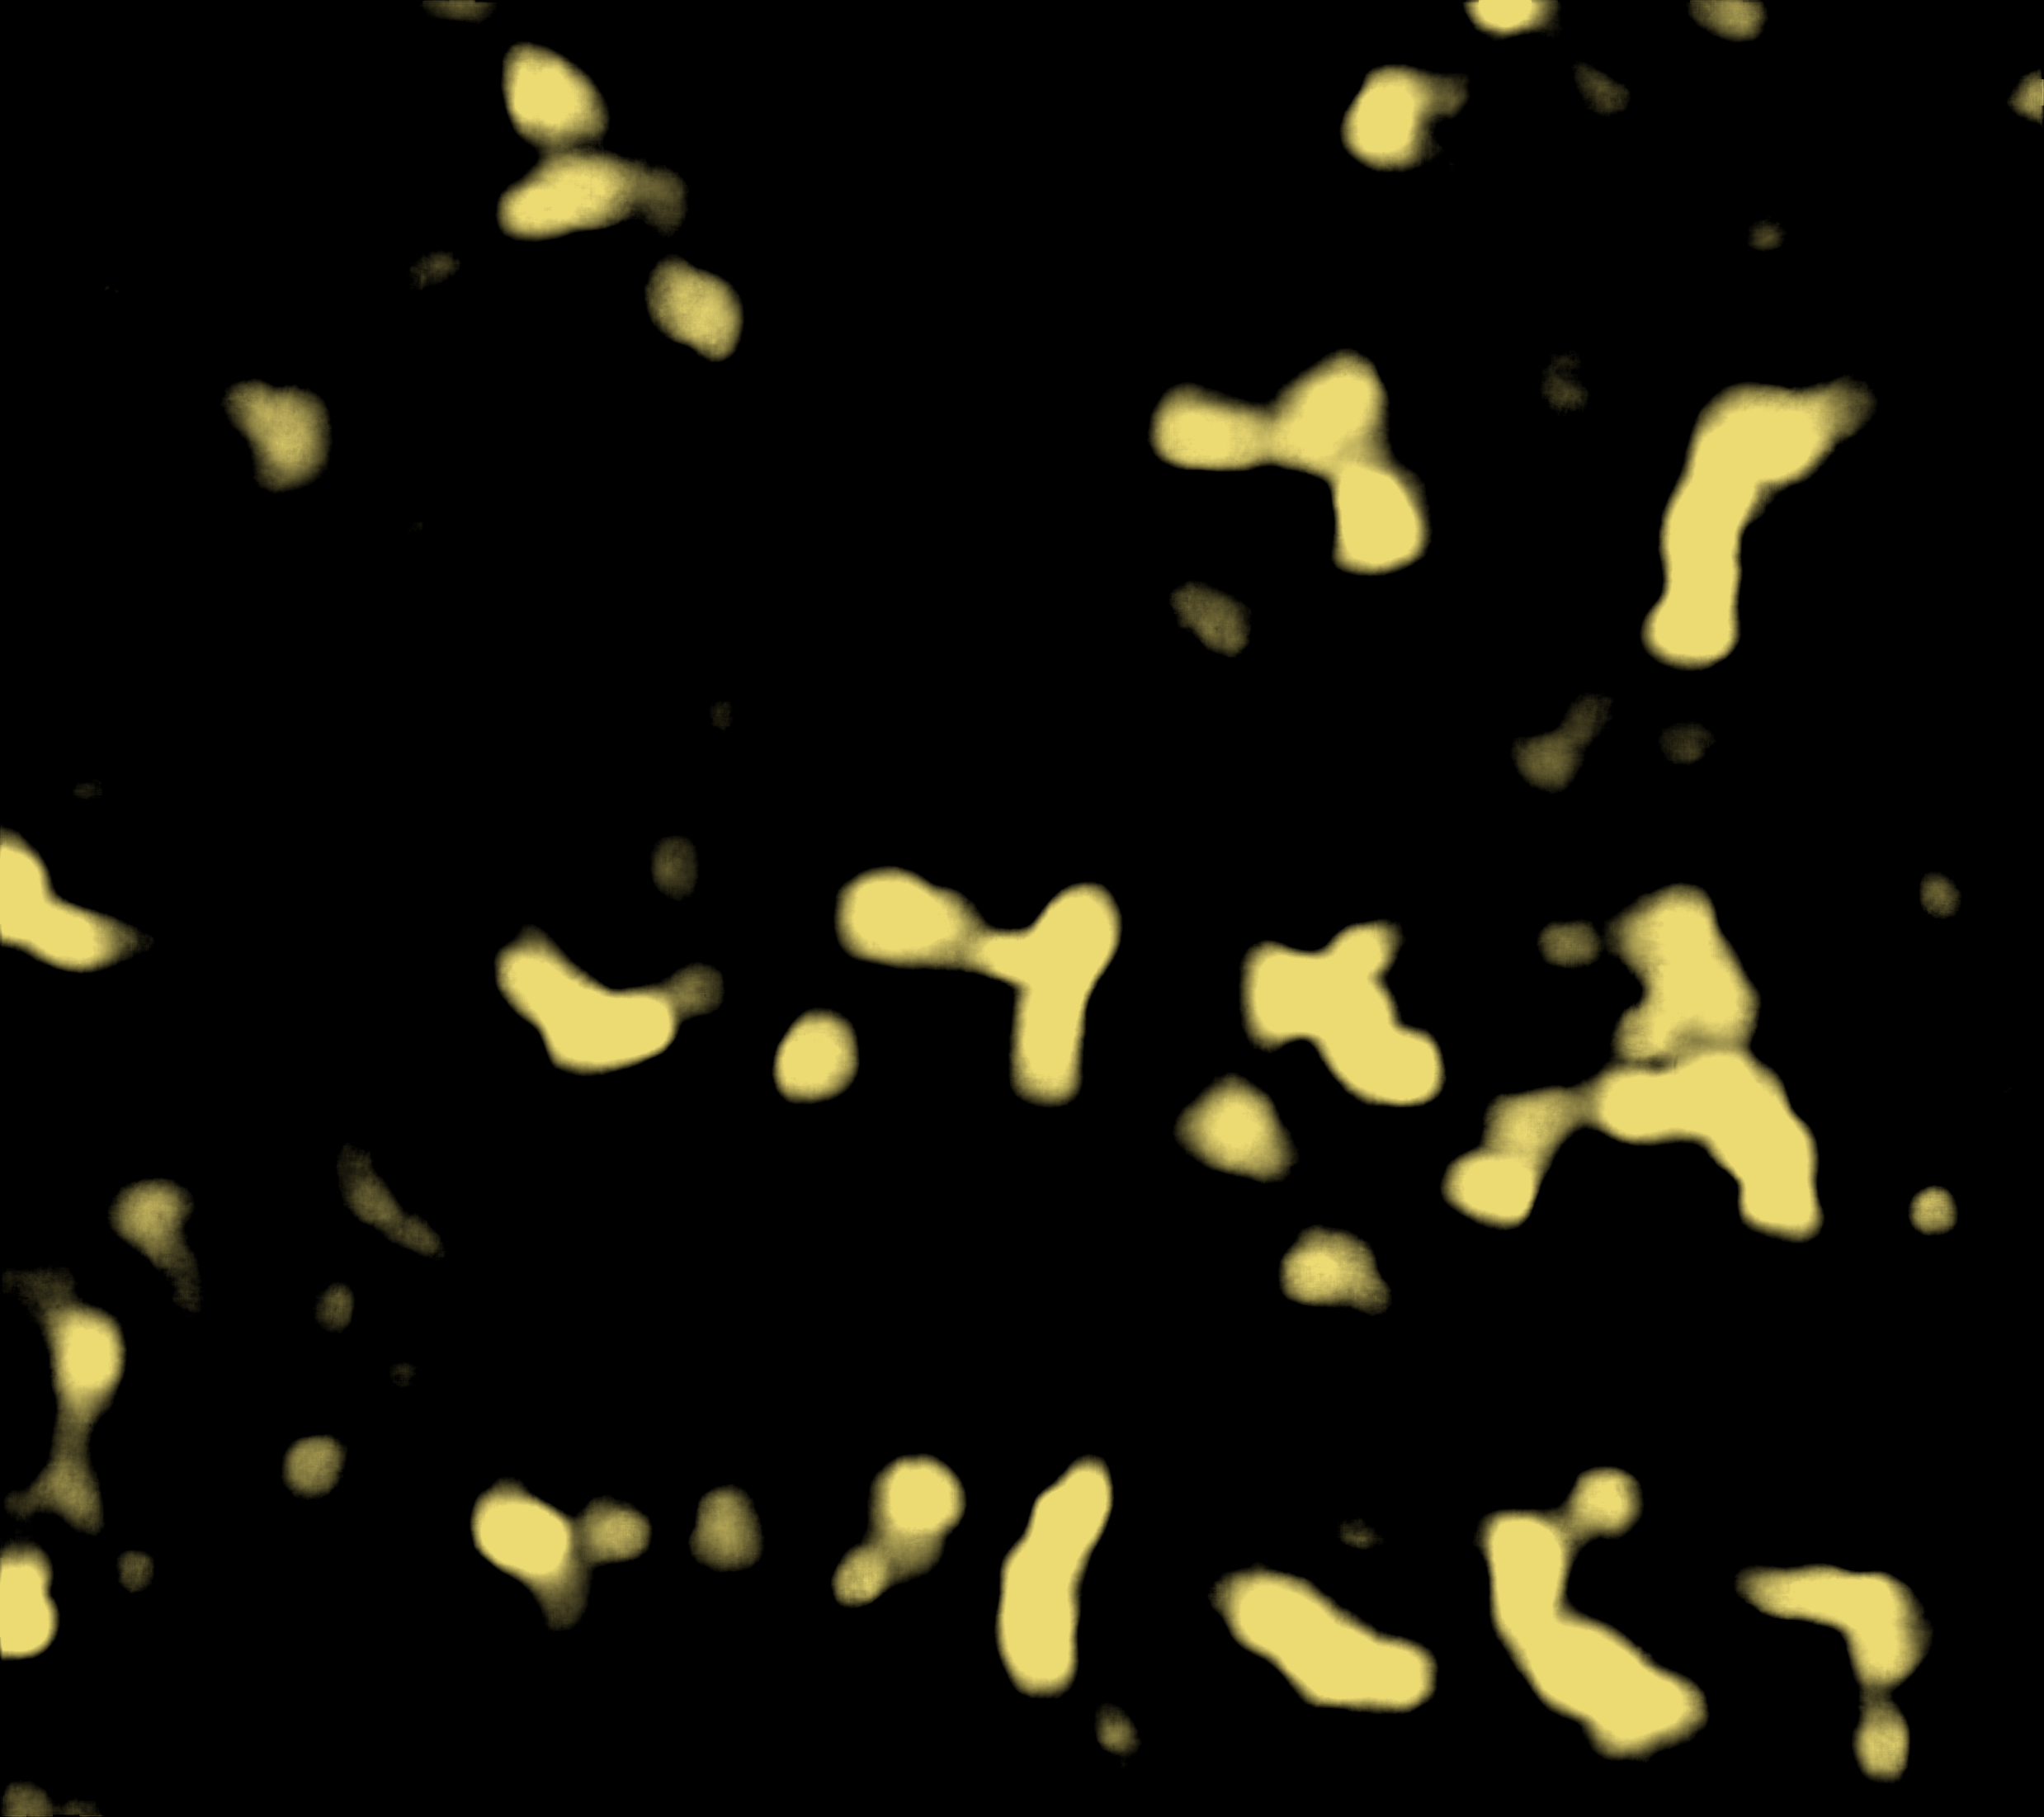
\includegraphics[width=122.48pt]{../figures/ag2/ag2_5_rectina-m1.png}}\end{minipage}}
\par\vspace{4pt}
\noindent\makebox[\columnwidth][c]{\begin{minipage}[t]{122.48pt}\centering\href{https://raw.githubusercontent.com/evilaliv3/vesuvius-challenge-pipeline/main/results/db27c806-rectina/src/figures/ag2/ag2_4_reader-v3.png}{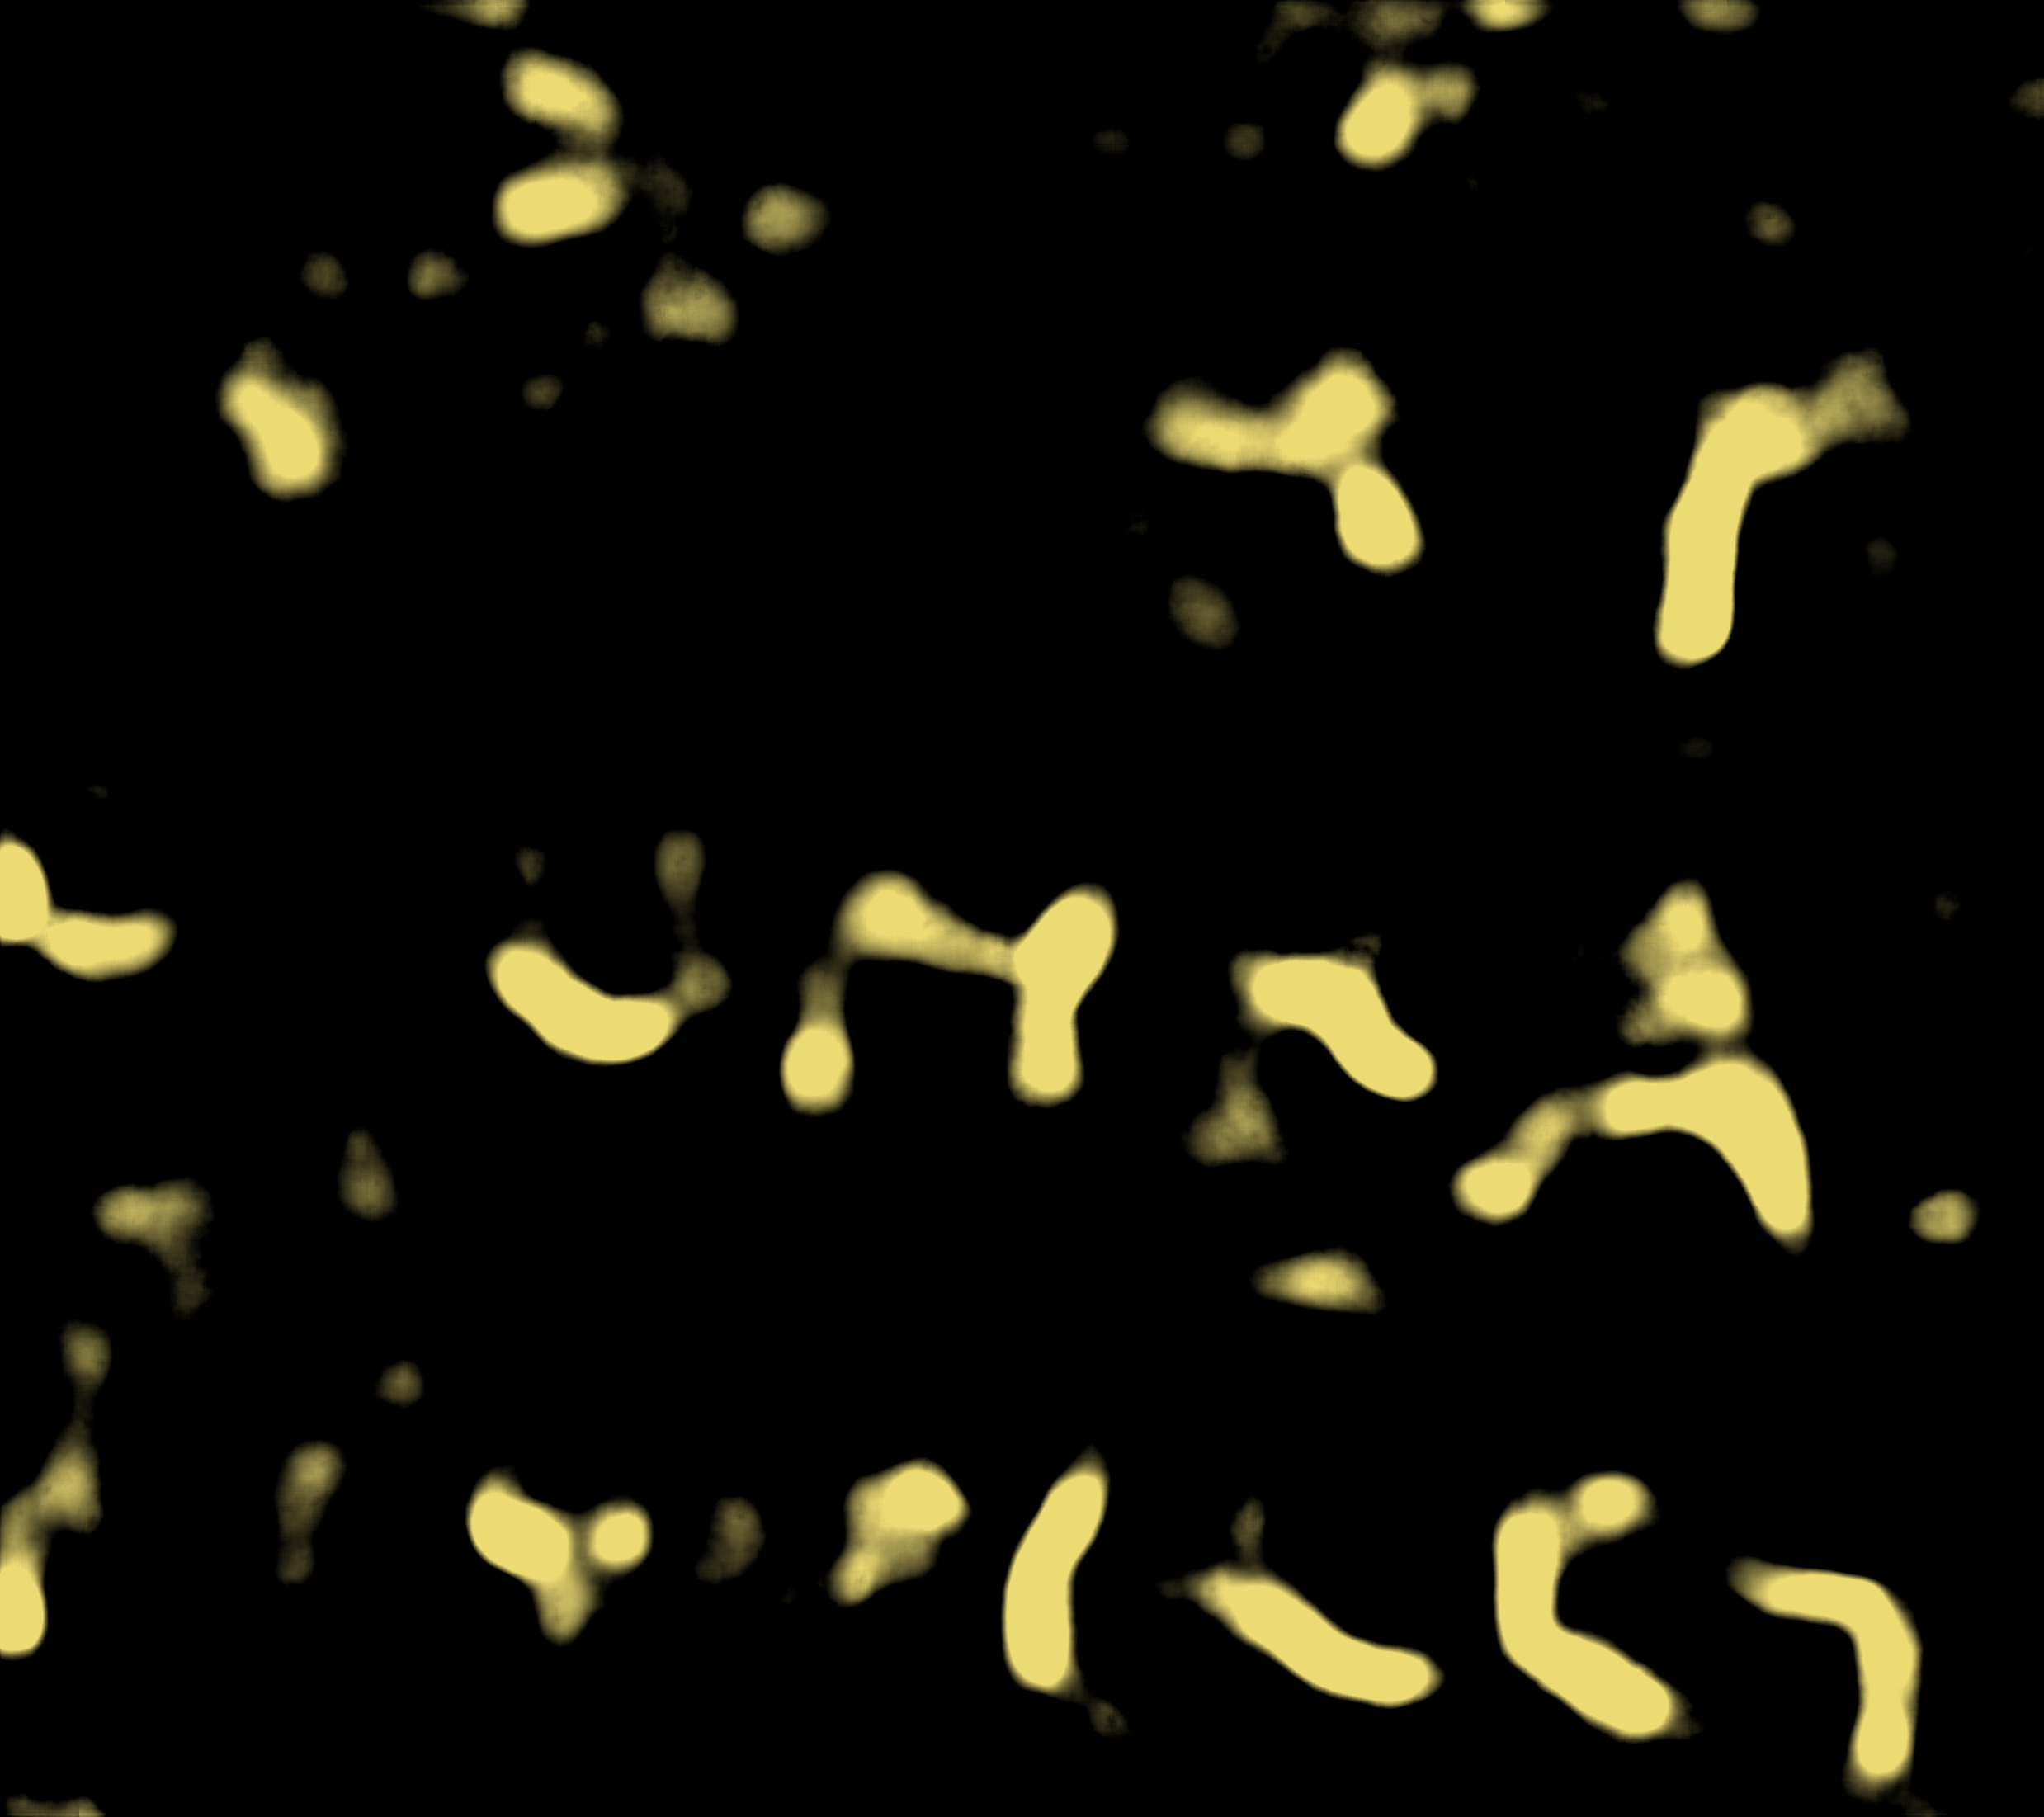
\includegraphics[width=122.48pt]{../figures/ag2/ag2_4_reader-v3.png}}\end{minipage}\hspace{2pt}\begin{minipage}[t]{122.48pt}\centering\href{https://raw.githubusercontent.com/evilaliv3/vesuvius-challenge-pipeline/main/results/db27c806-rectina/src/figures/ag2/ag2_6_rectina-m2.png}{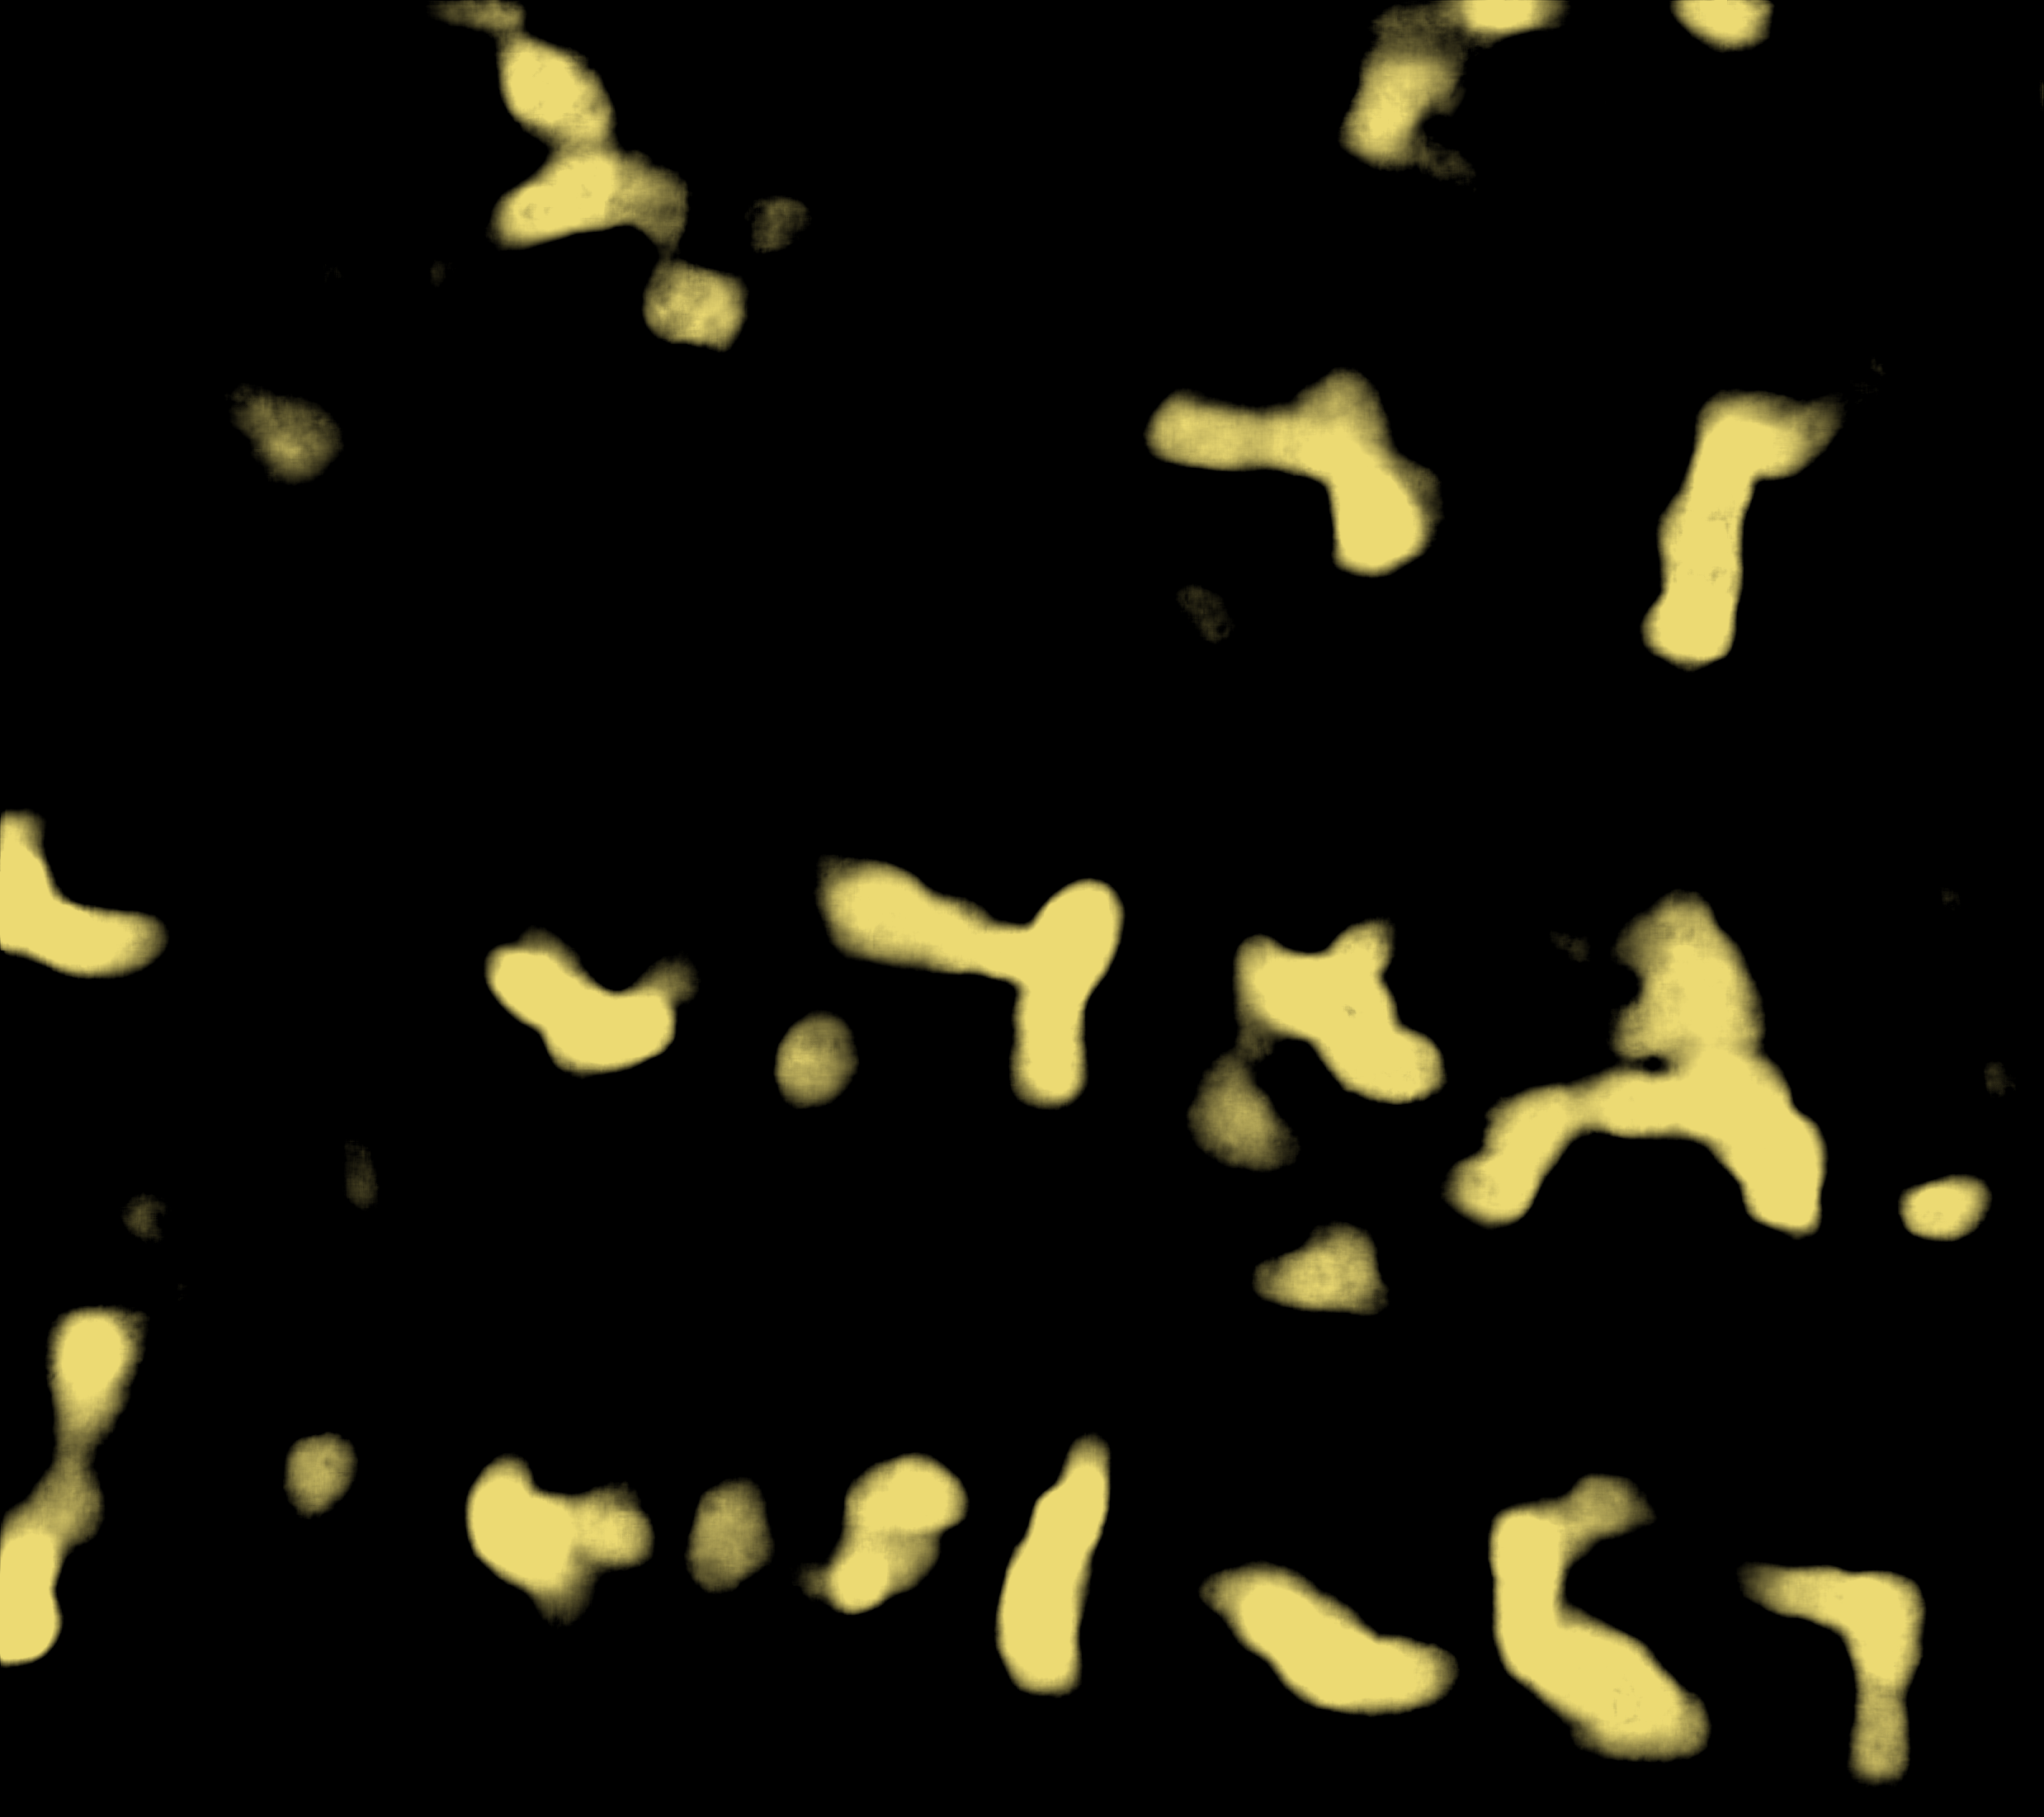
\includegraphics[width=122.48pt]{../figures/ag2/ag2_6_rectina-m2.png}}\end{minipage}}
\caption{Control unit 0841 ag2, three rows of two panels. Row 1: left, Texture; right, Labels. Row 2: left, Reader v2; right, Rectina m1 (display windows: Reader v2 0.404870 to 0.589240 (ramp); Rectina m1 0.560881 to 0.723274 (ramp)). Row 3: left, Reader v3; right, Rectina m2 (display windows: Reader v3 0.431564 to 0.660926 (ramp); Rectina m2 0.615411 to 0.768217 (ramp)). Each map is stretched between its own percentiles. Reader and model stand side by side in the rows 2 and 3.}
\end{figure}

\begin{figure}[!tbp]
\centering
\noindent\makebox[\columnwidth][c]{\begin{minipage}[t]{122.48pt}\centering\href{https://raw.githubusercontent.com/evilaliv3/vesuvius-challenge-pipeline/main/results/db27c806-rectina/src/figures/w00/w00_1_texture.png}{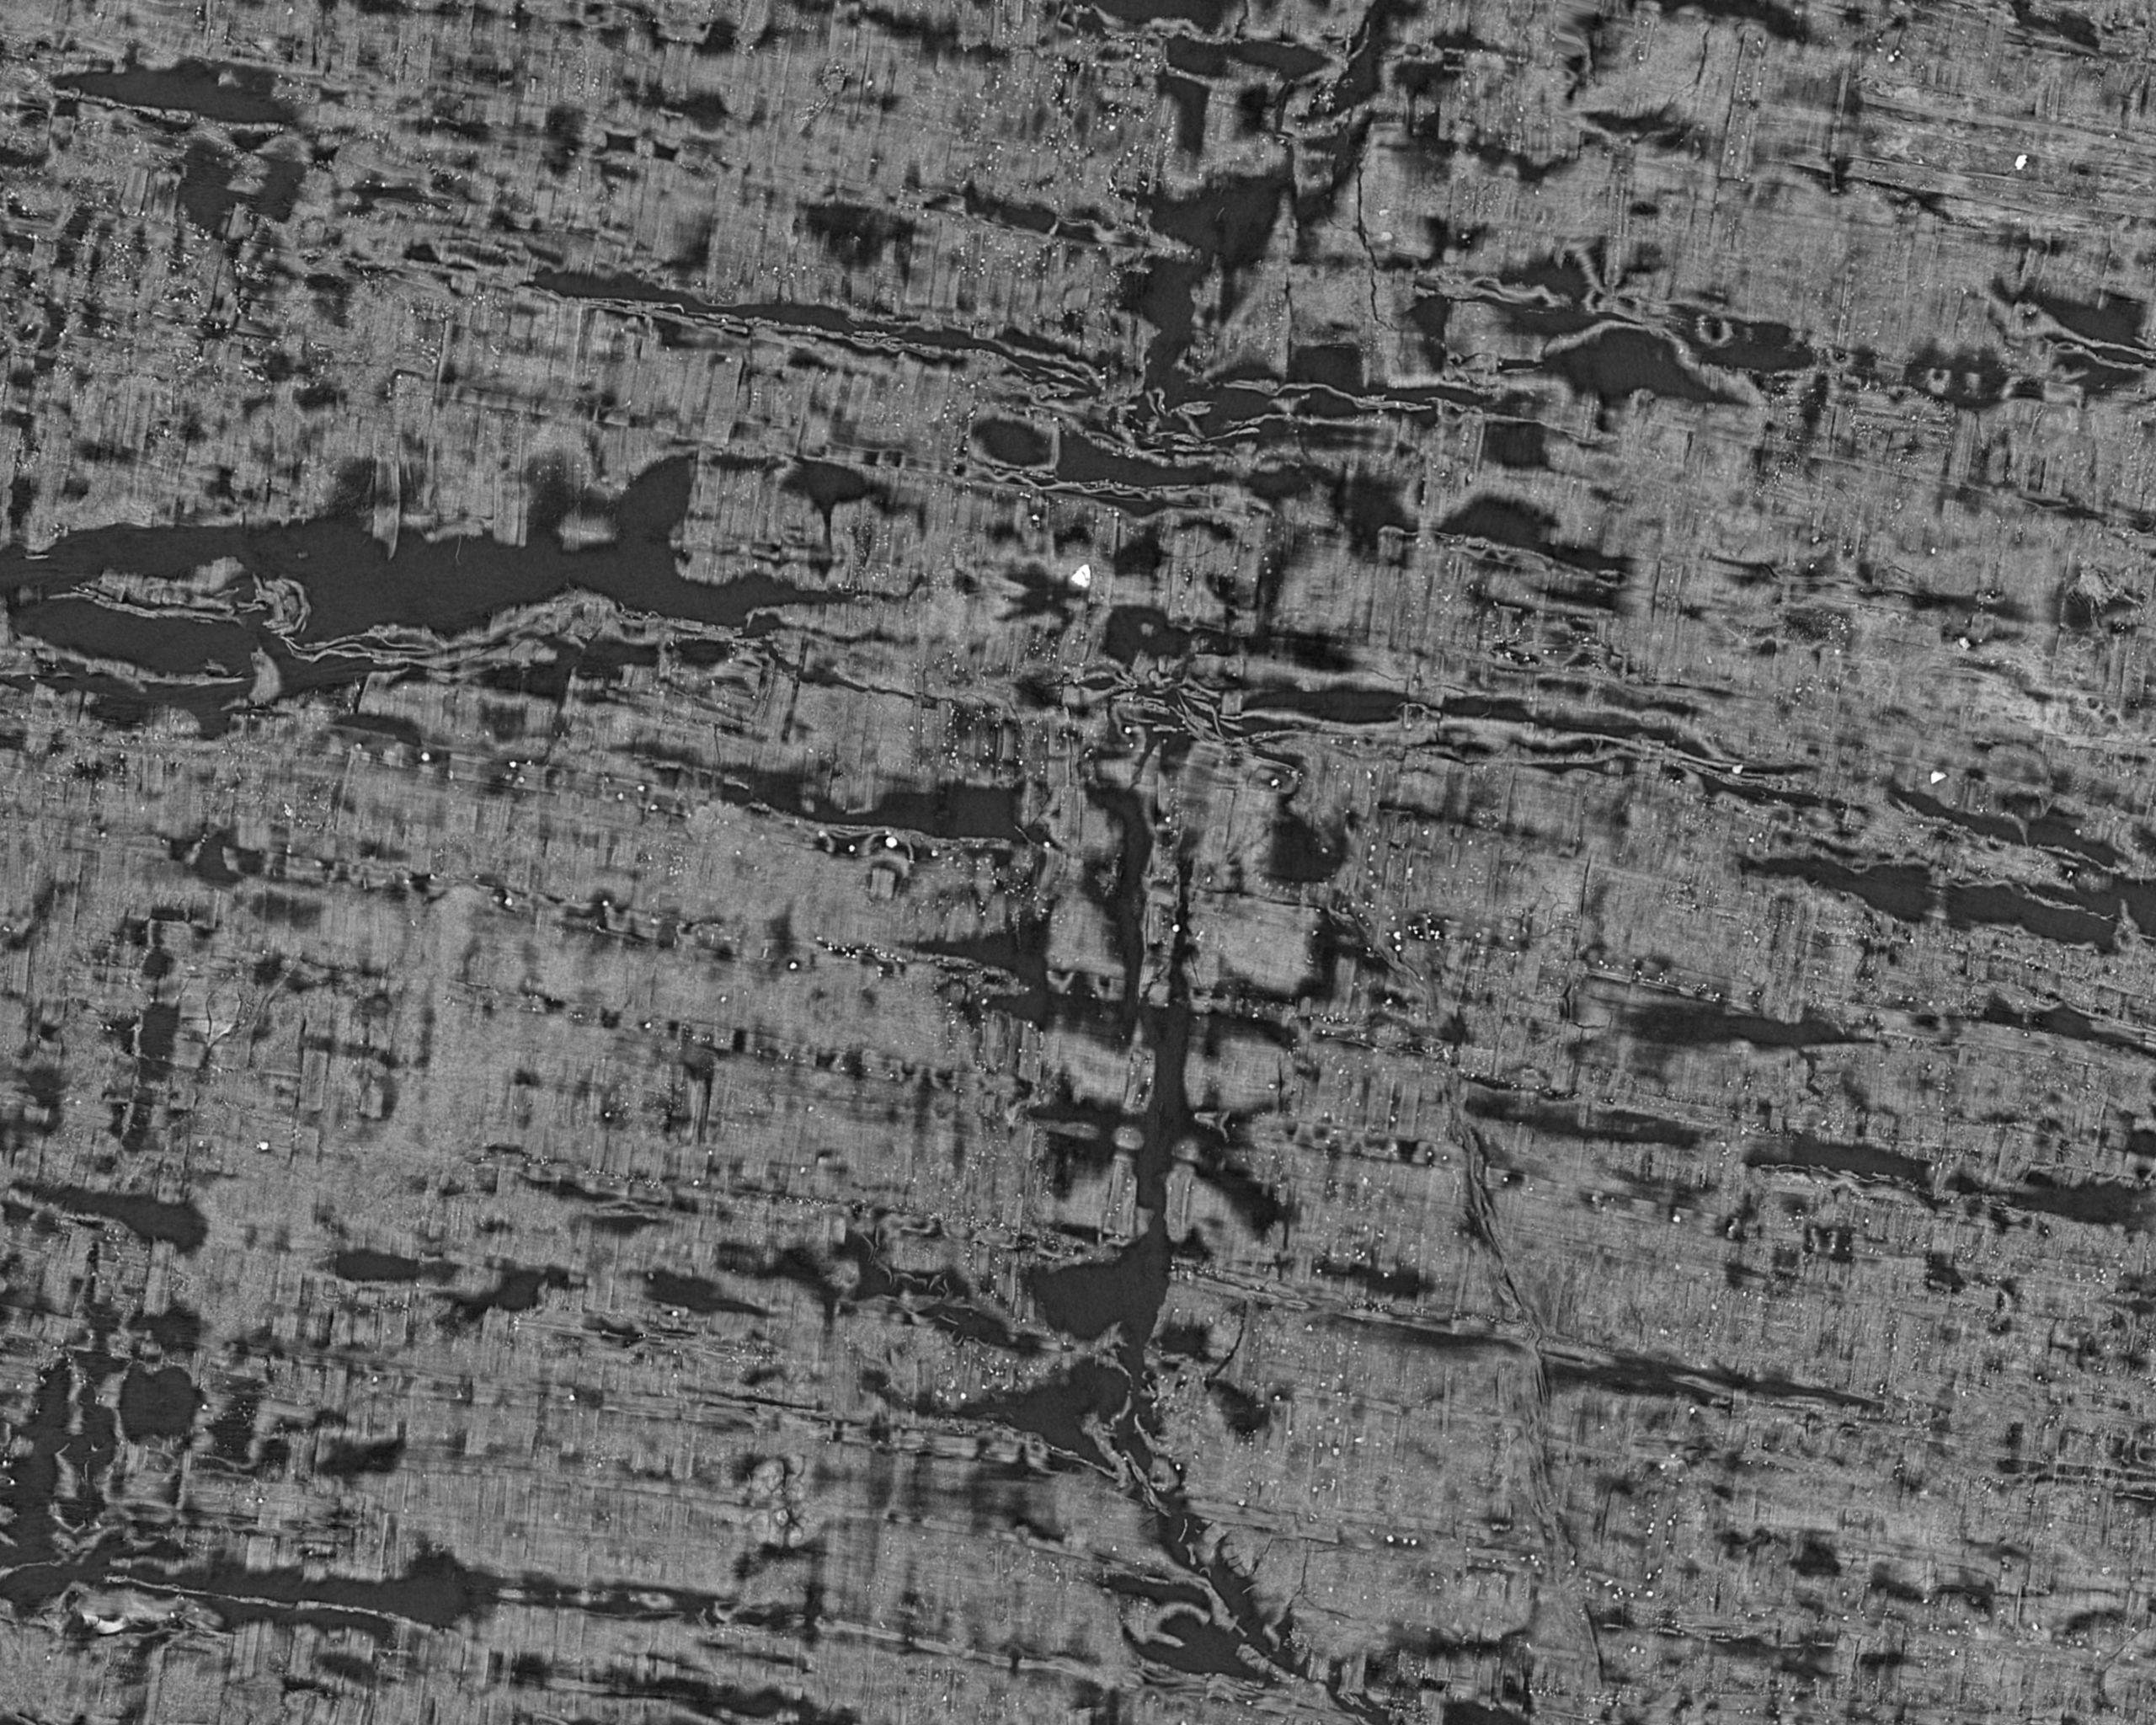
\includegraphics[width=122.48pt]{../figures/w00/w00_1_texture.png}}\end{minipage}\hspace{2pt}\begin{minipage}[t]{122.48pt}\centering\href{https://raw.githubusercontent.com/evilaliv3/vesuvius-challenge-pipeline/main/results/db27c806-rectina/src/figures/w00/w00_2_labels.png}{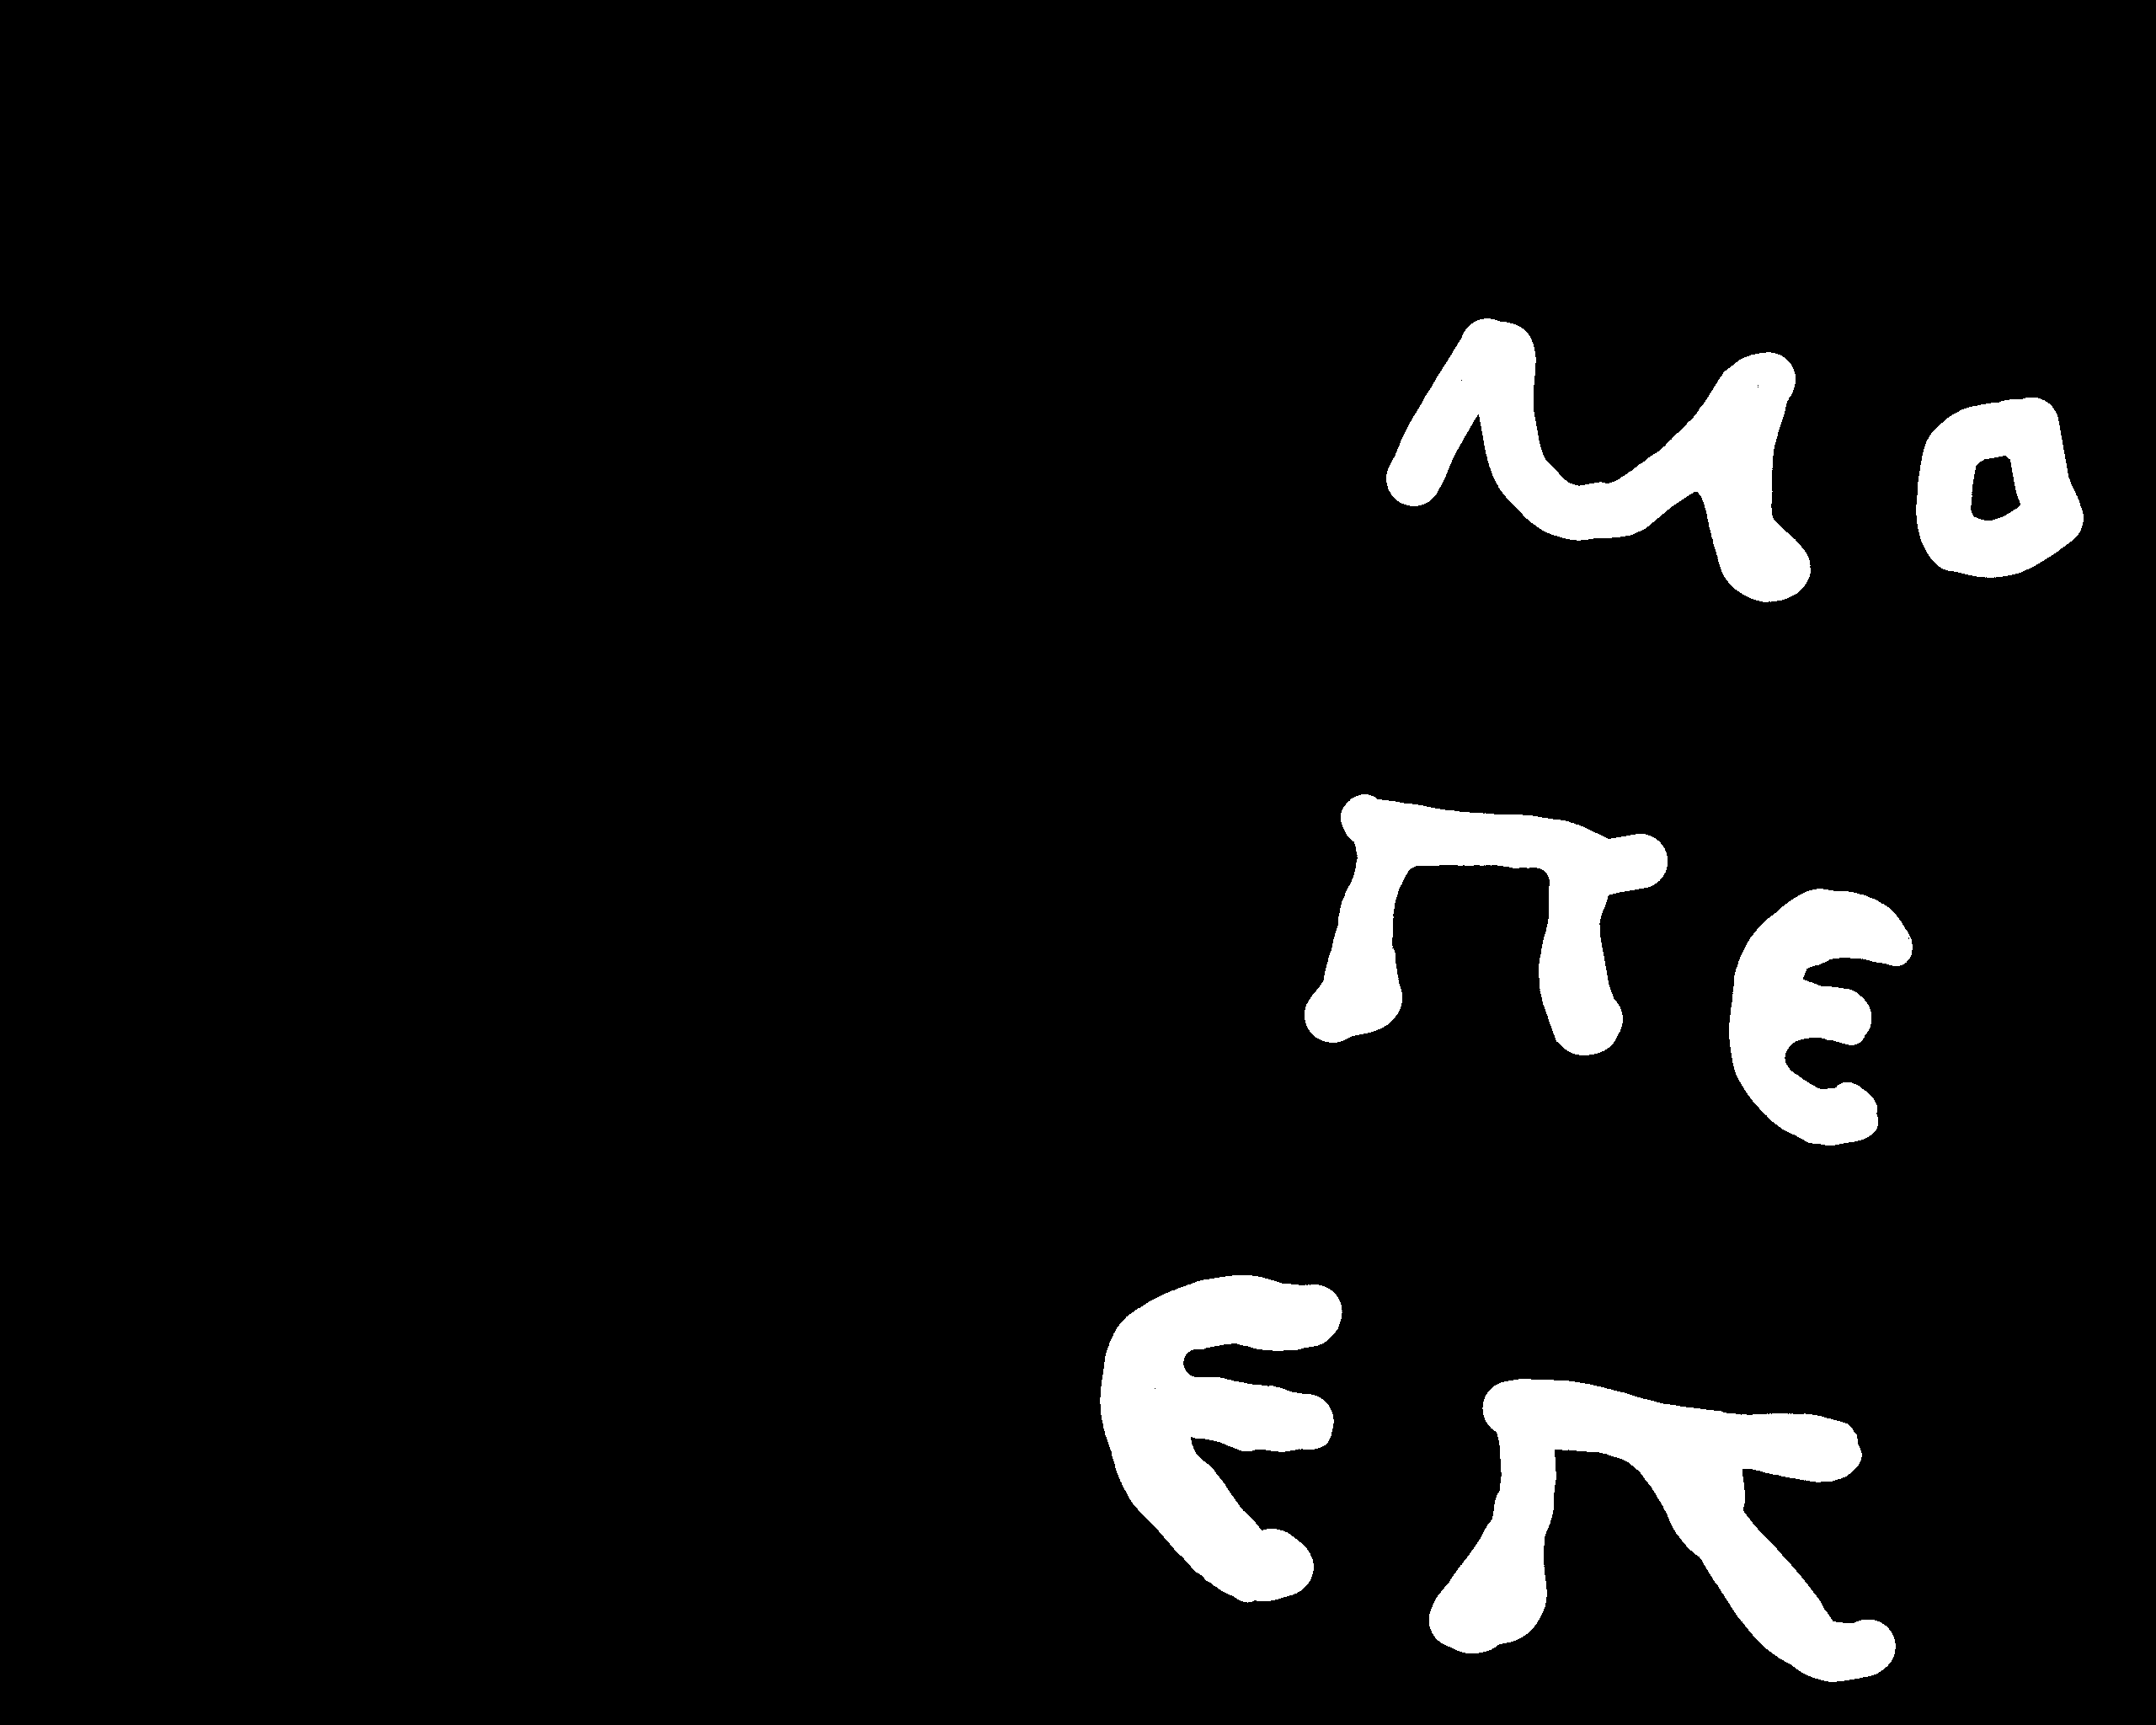
\includegraphics[width=122.48pt]{../figures/w00/w00_2_labels.png}}\end{minipage}}
\par\vspace{4pt}
\noindent\makebox[\columnwidth][c]{\begin{minipage}[t]{122.48pt}\centering\href{https://raw.githubusercontent.com/evilaliv3/vesuvius-challenge-pipeline/main/results/db27c806-rectina/src/figures/w00/w00_3_reader-v2.png}{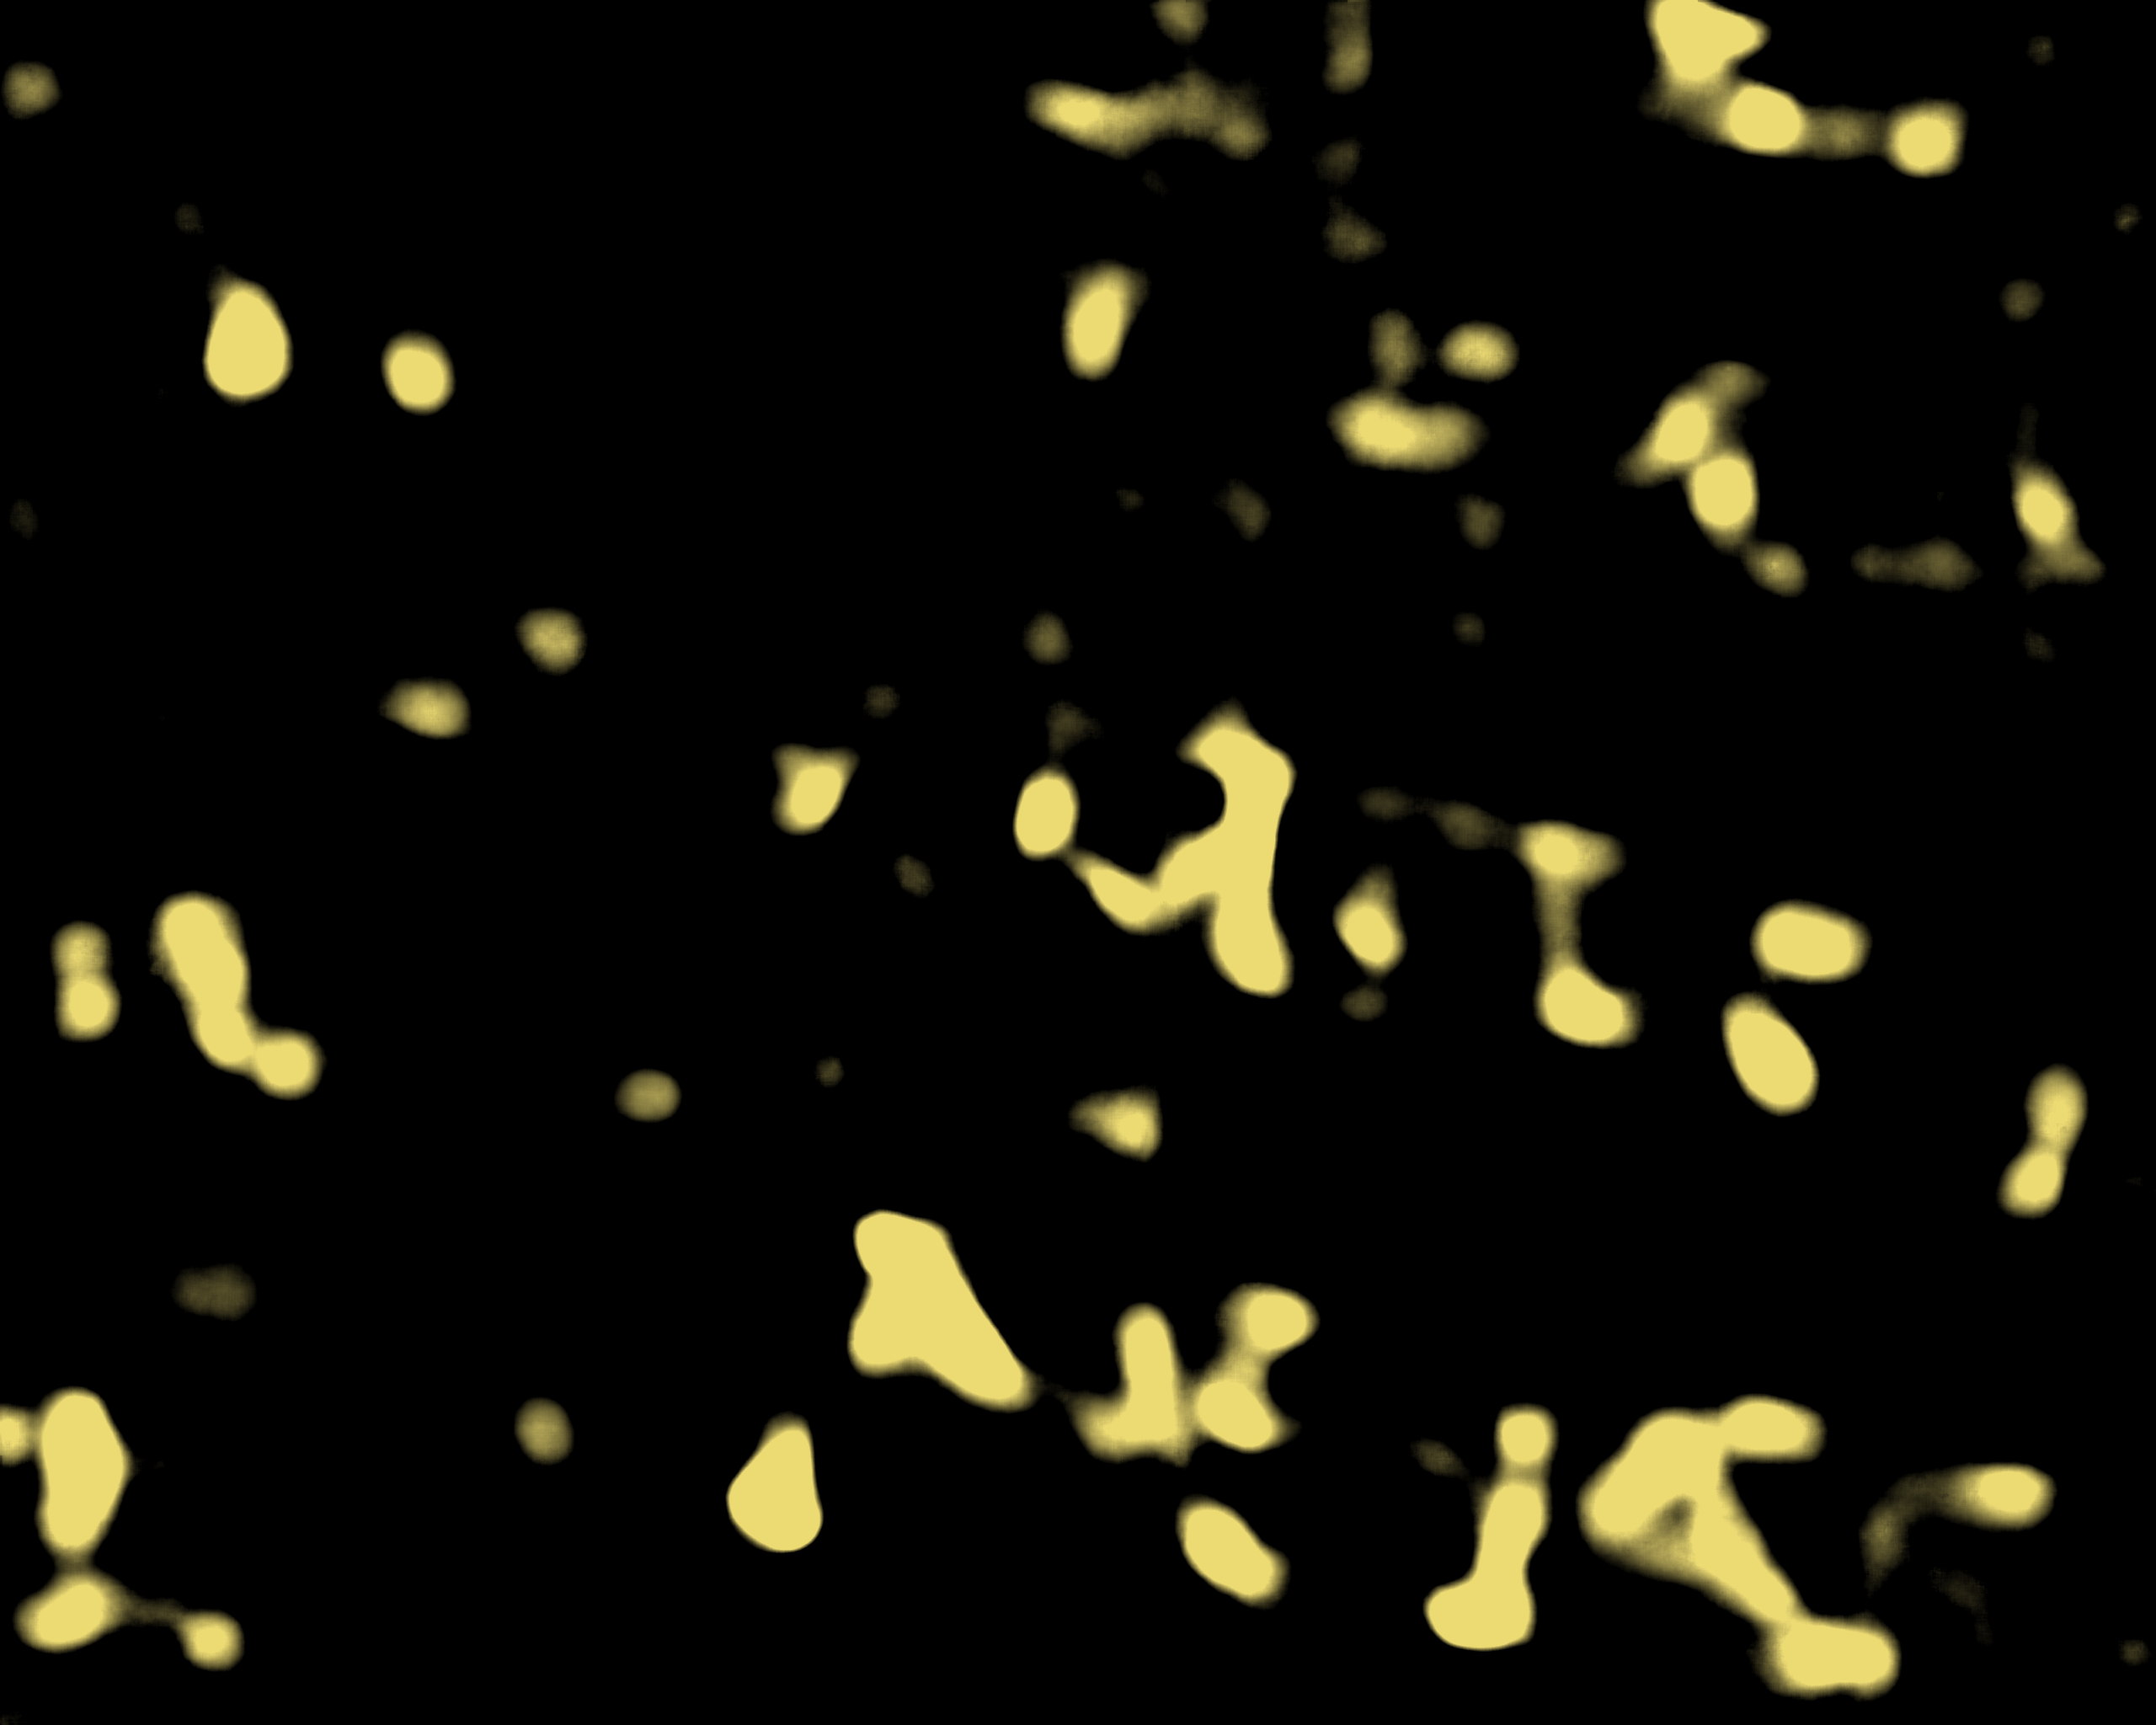
\includegraphics[width=122.48pt]{../figures/w00/w00_3_reader-v2.png}}\end{minipage}\hspace{2pt}\begin{minipage}[t]{122.48pt}\centering\href{https://raw.githubusercontent.com/evilaliv3/vesuvius-challenge-pipeline/main/results/db27c806-rectina/src/figures/w00/w00_5_rectina-m1.png}{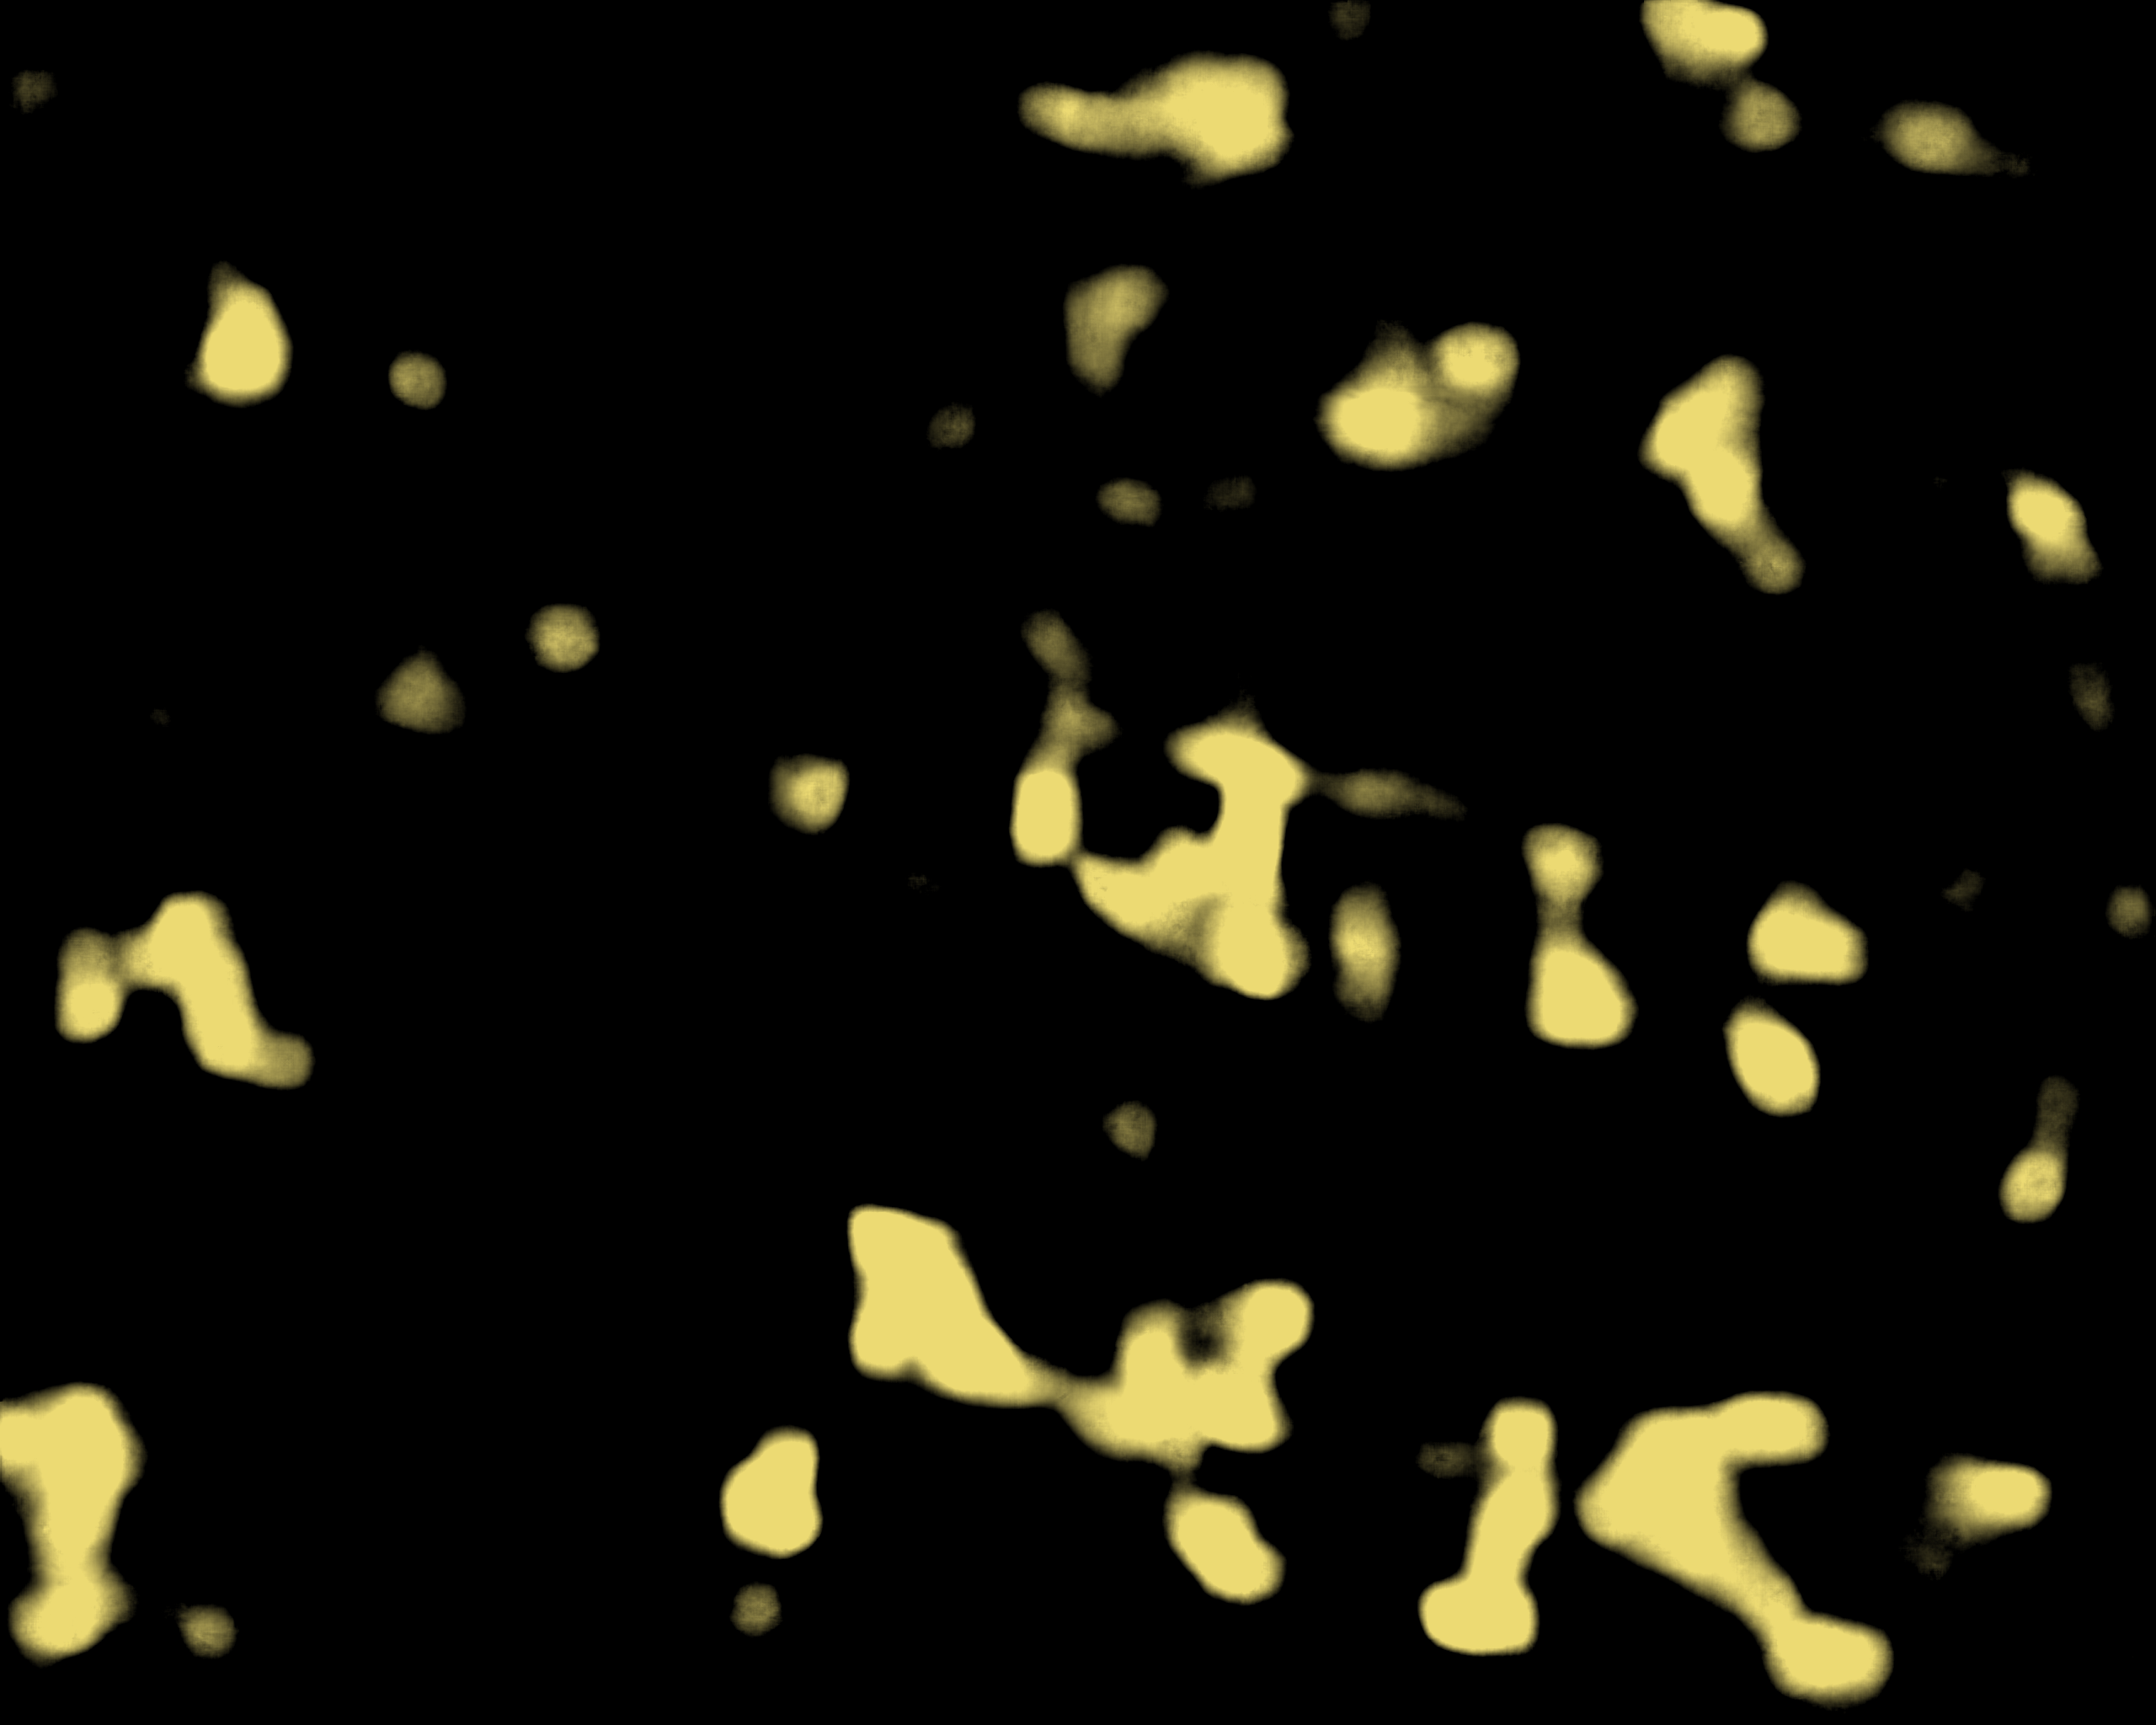
\includegraphics[width=122.48pt]{../figures/w00/w00_5_rectina-m1.png}}\end{minipage}}
\par\vspace{4pt}
\noindent\makebox[\columnwidth][c]{\begin{minipage}[t]{122.48pt}\centering\href{https://raw.githubusercontent.com/evilaliv3/vesuvius-challenge-pipeline/main/results/db27c806-rectina/src/figures/w00/w00_4_reader-v3.png}{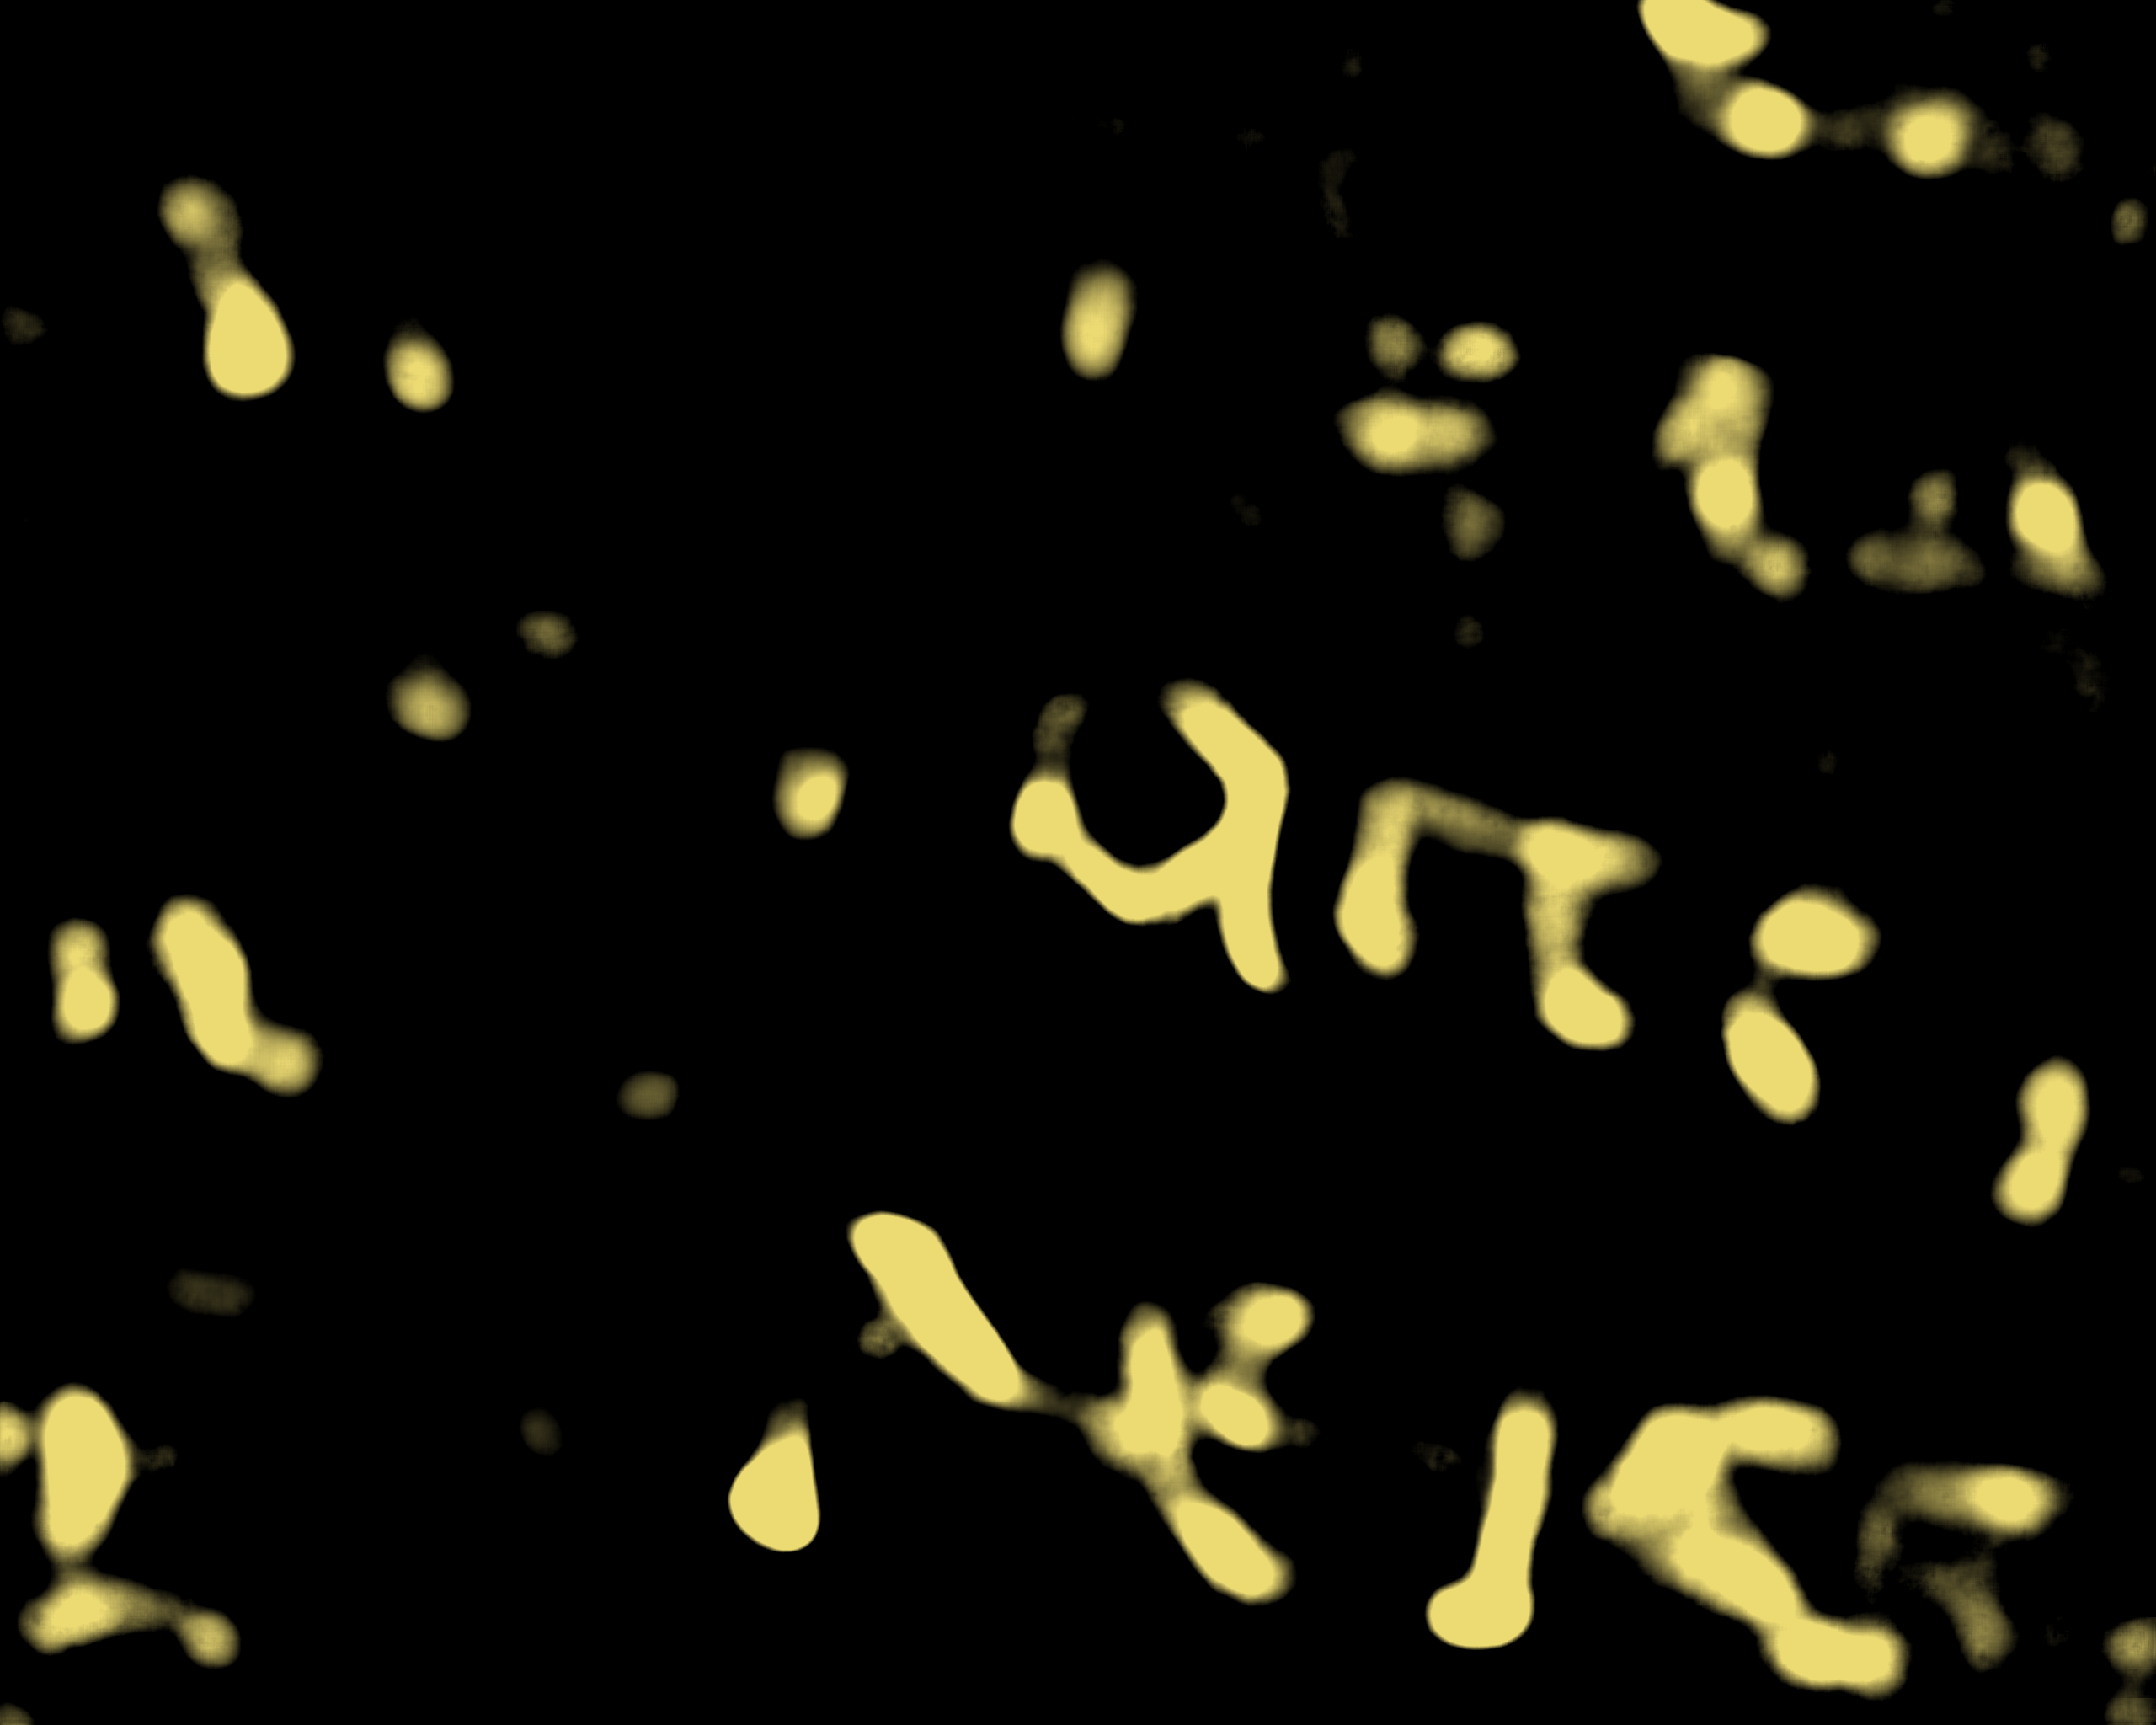
\includegraphics[width=122.48pt]{../figures/w00/w00_4_reader-v3.png}}\end{minipage}\hspace{2pt}\begin{minipage}[t]{122.48pt}\centering\href{https://raw.githubusercontent.com/evilaliv3/vesuvius-challenge-pipeline/main/results/db27c806-rectina/src/figures/w00/w00_6_rectina-m2.png}{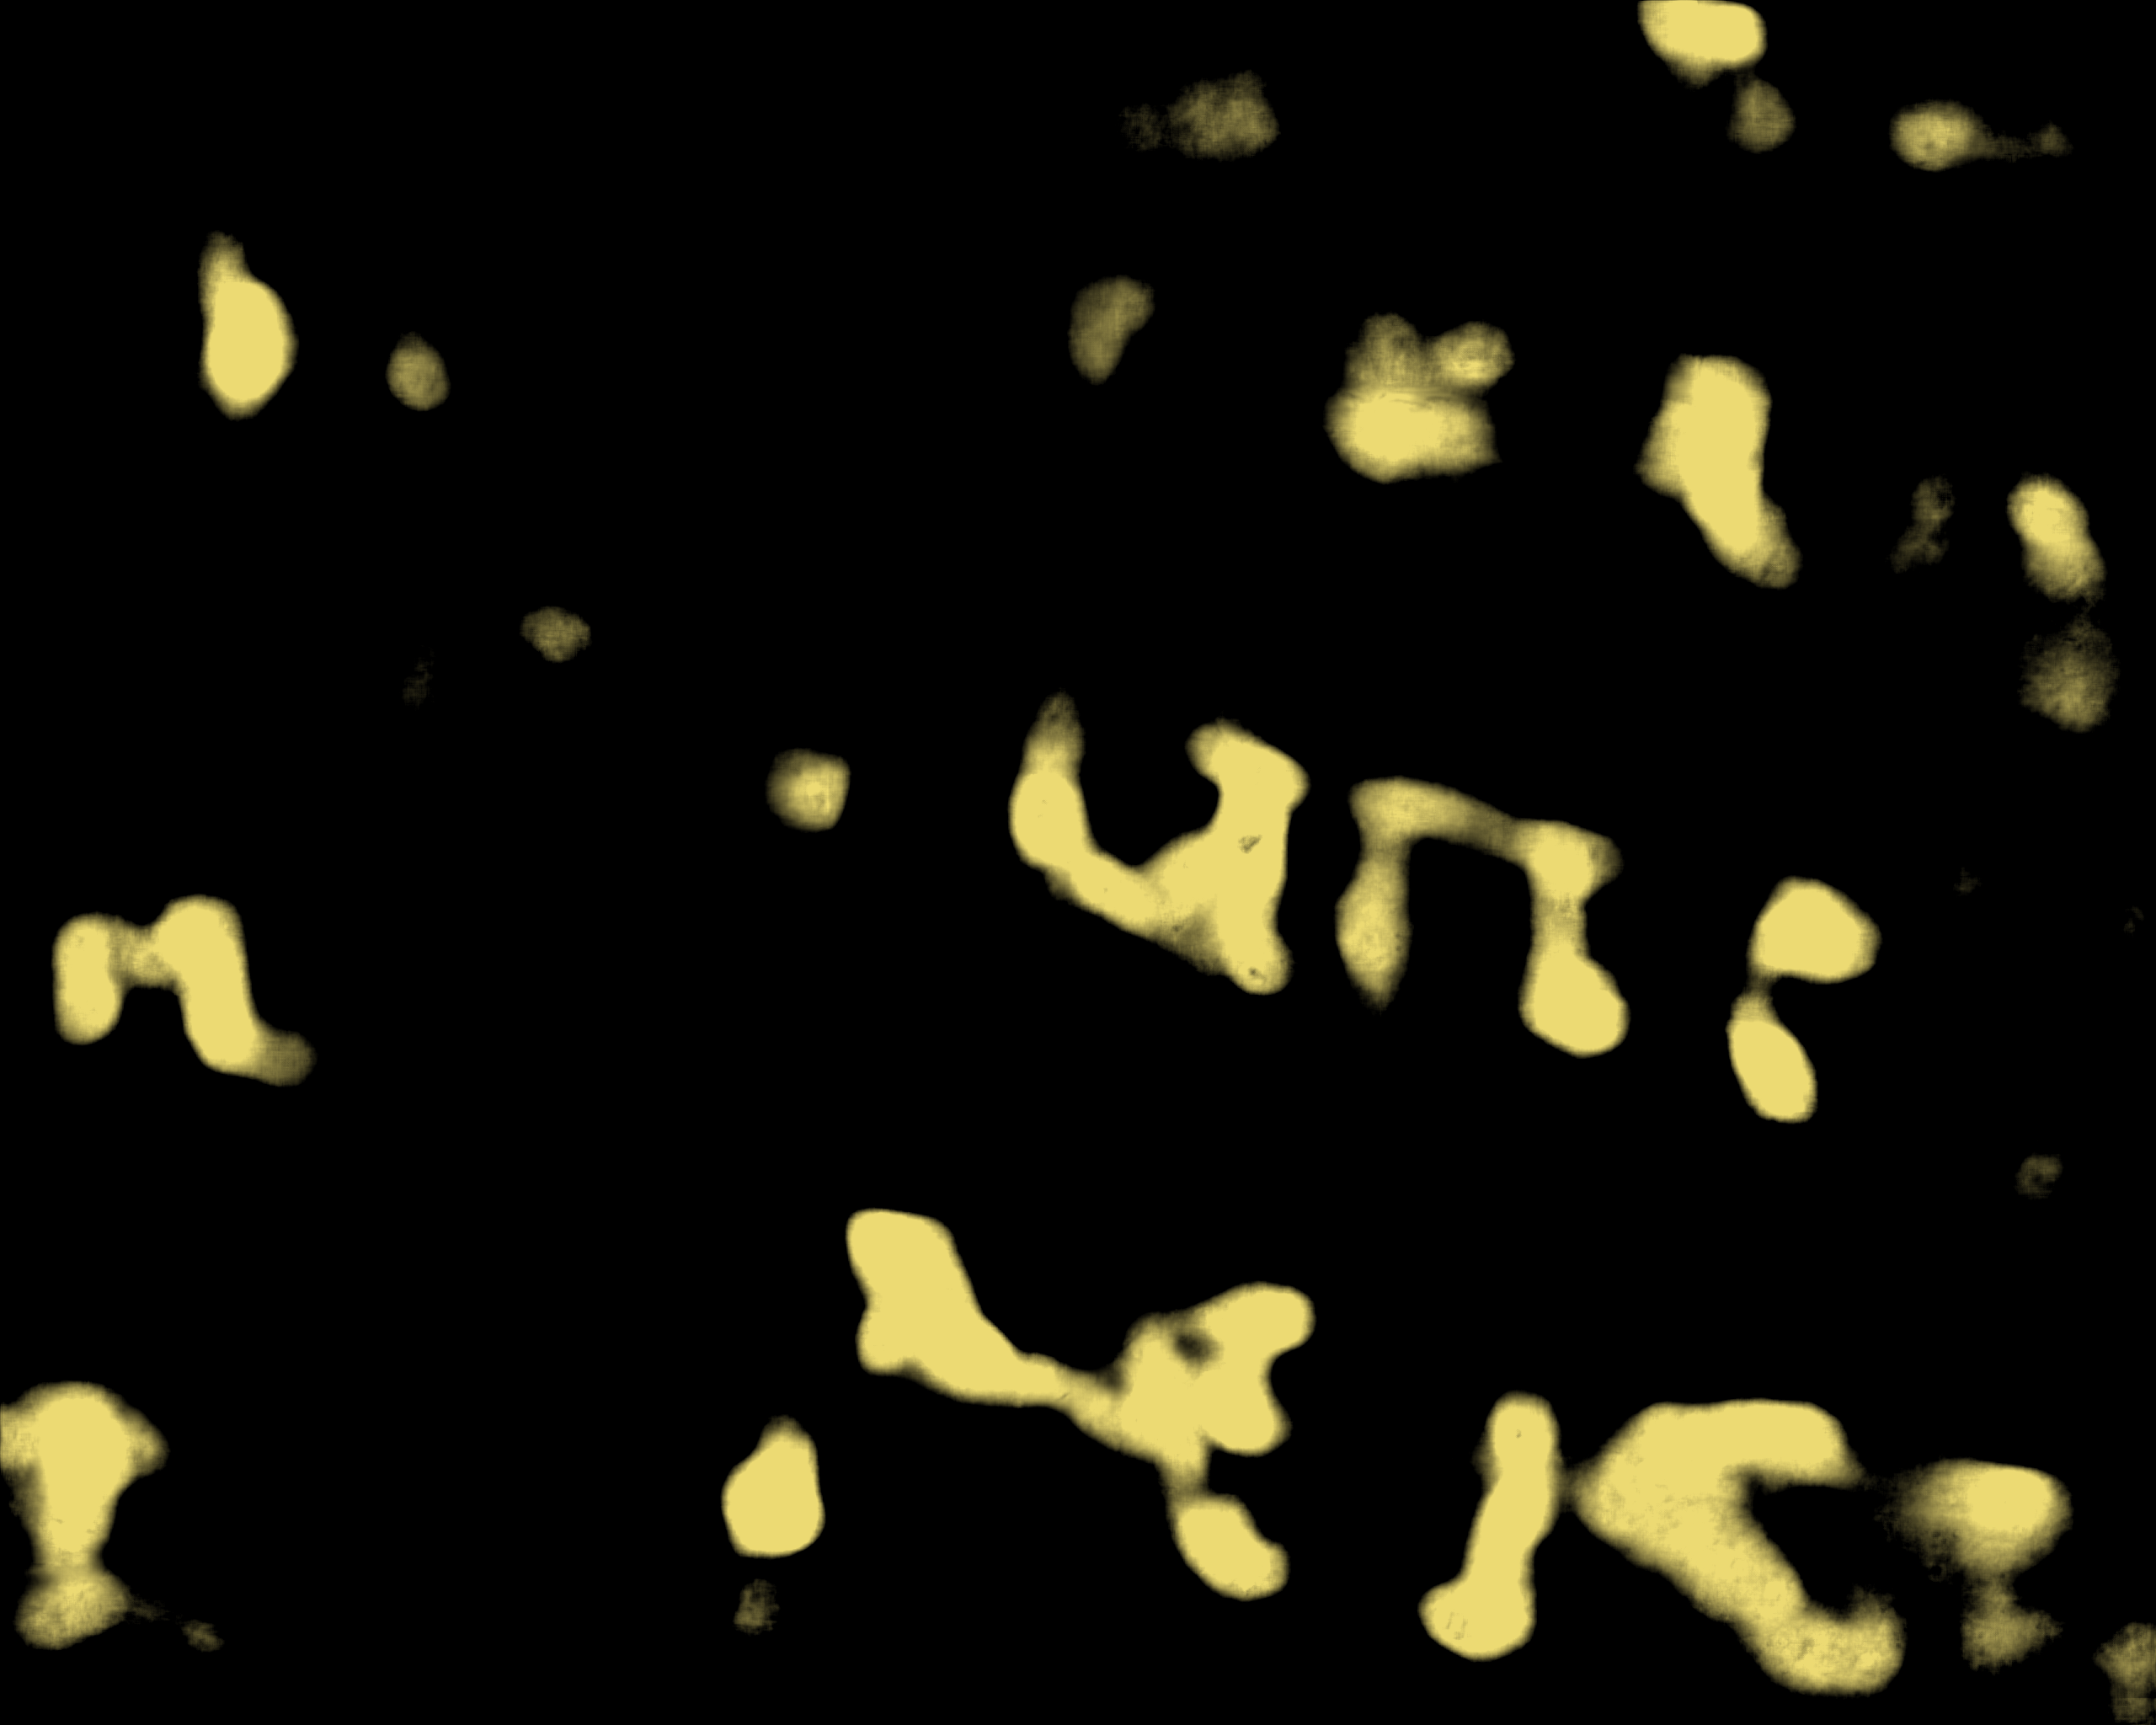
\includegraphics[width=122.48pt]{../figures/w00/w00_6_rectina-m2.png}}\end{minipage}}
\caption{Control unit 0841 w00, three rows of two panels. Row 1: left, Texture; right, Labels. Row 2: left, Reader v2; right, Rectina m1 (display windows: Reader v2 0.419276 to 0.595756 (ramp); Rectina m1 0.577431 to 0.724182 (ramp)). Row 3: left, Reader v3; right, Rectina m2 (display windows: Reader v3 0.454060 to 0.672485 (ramp); Rectina m2 0.650603 to 0.768363 (ramp)). Each map is stretched between its own percentiles. Reader and model stand side by side in the rows 2 and 3.}
\end{figure}

\begin{figure}[!tbp]
\centering
\noindent\makebox[\columnwidth][c]{\begin{minipage}[t]{122.48pt}\centering\href{https://raw.githubusercontent.com/evilaliv3/vesuvius-challenge-pipeline/main/results/db27c806-rectina/src/figures/0343/0343_1_texture.png}{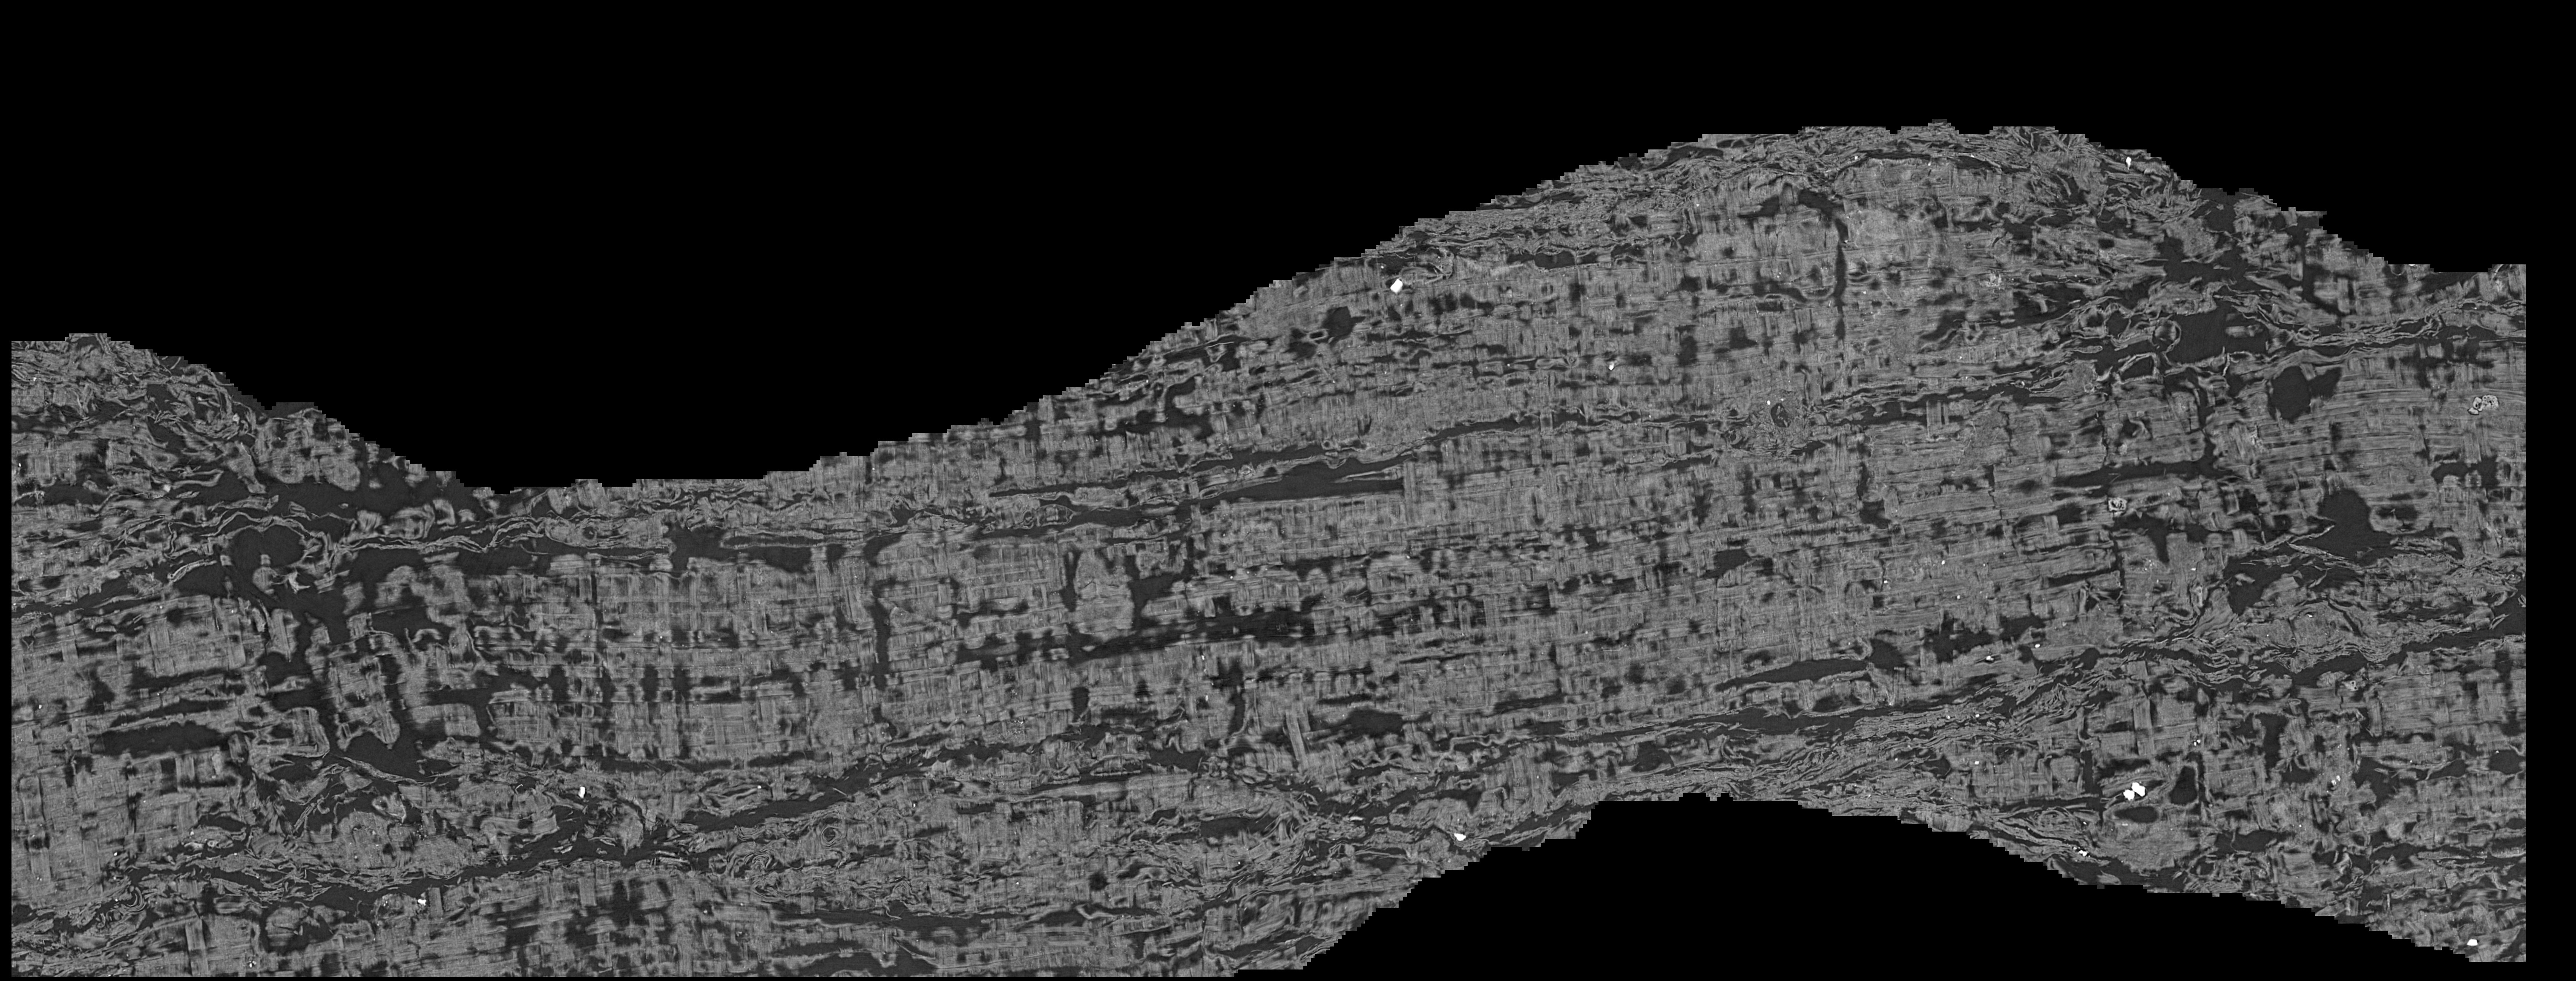
\includegraphics[width=122.48pt]{../figures/0343/0343_1_texture.png}}\end{minipage}\hspace{2pt}\begin{minipage}[t]{122.48pt}\centering\href{https://raw.githubusercontent.com/evilaliv3/vesuvius-challenge-pipeline/main/results/db27c806-rectina/src/figures/0343/0343_2_labels.png}{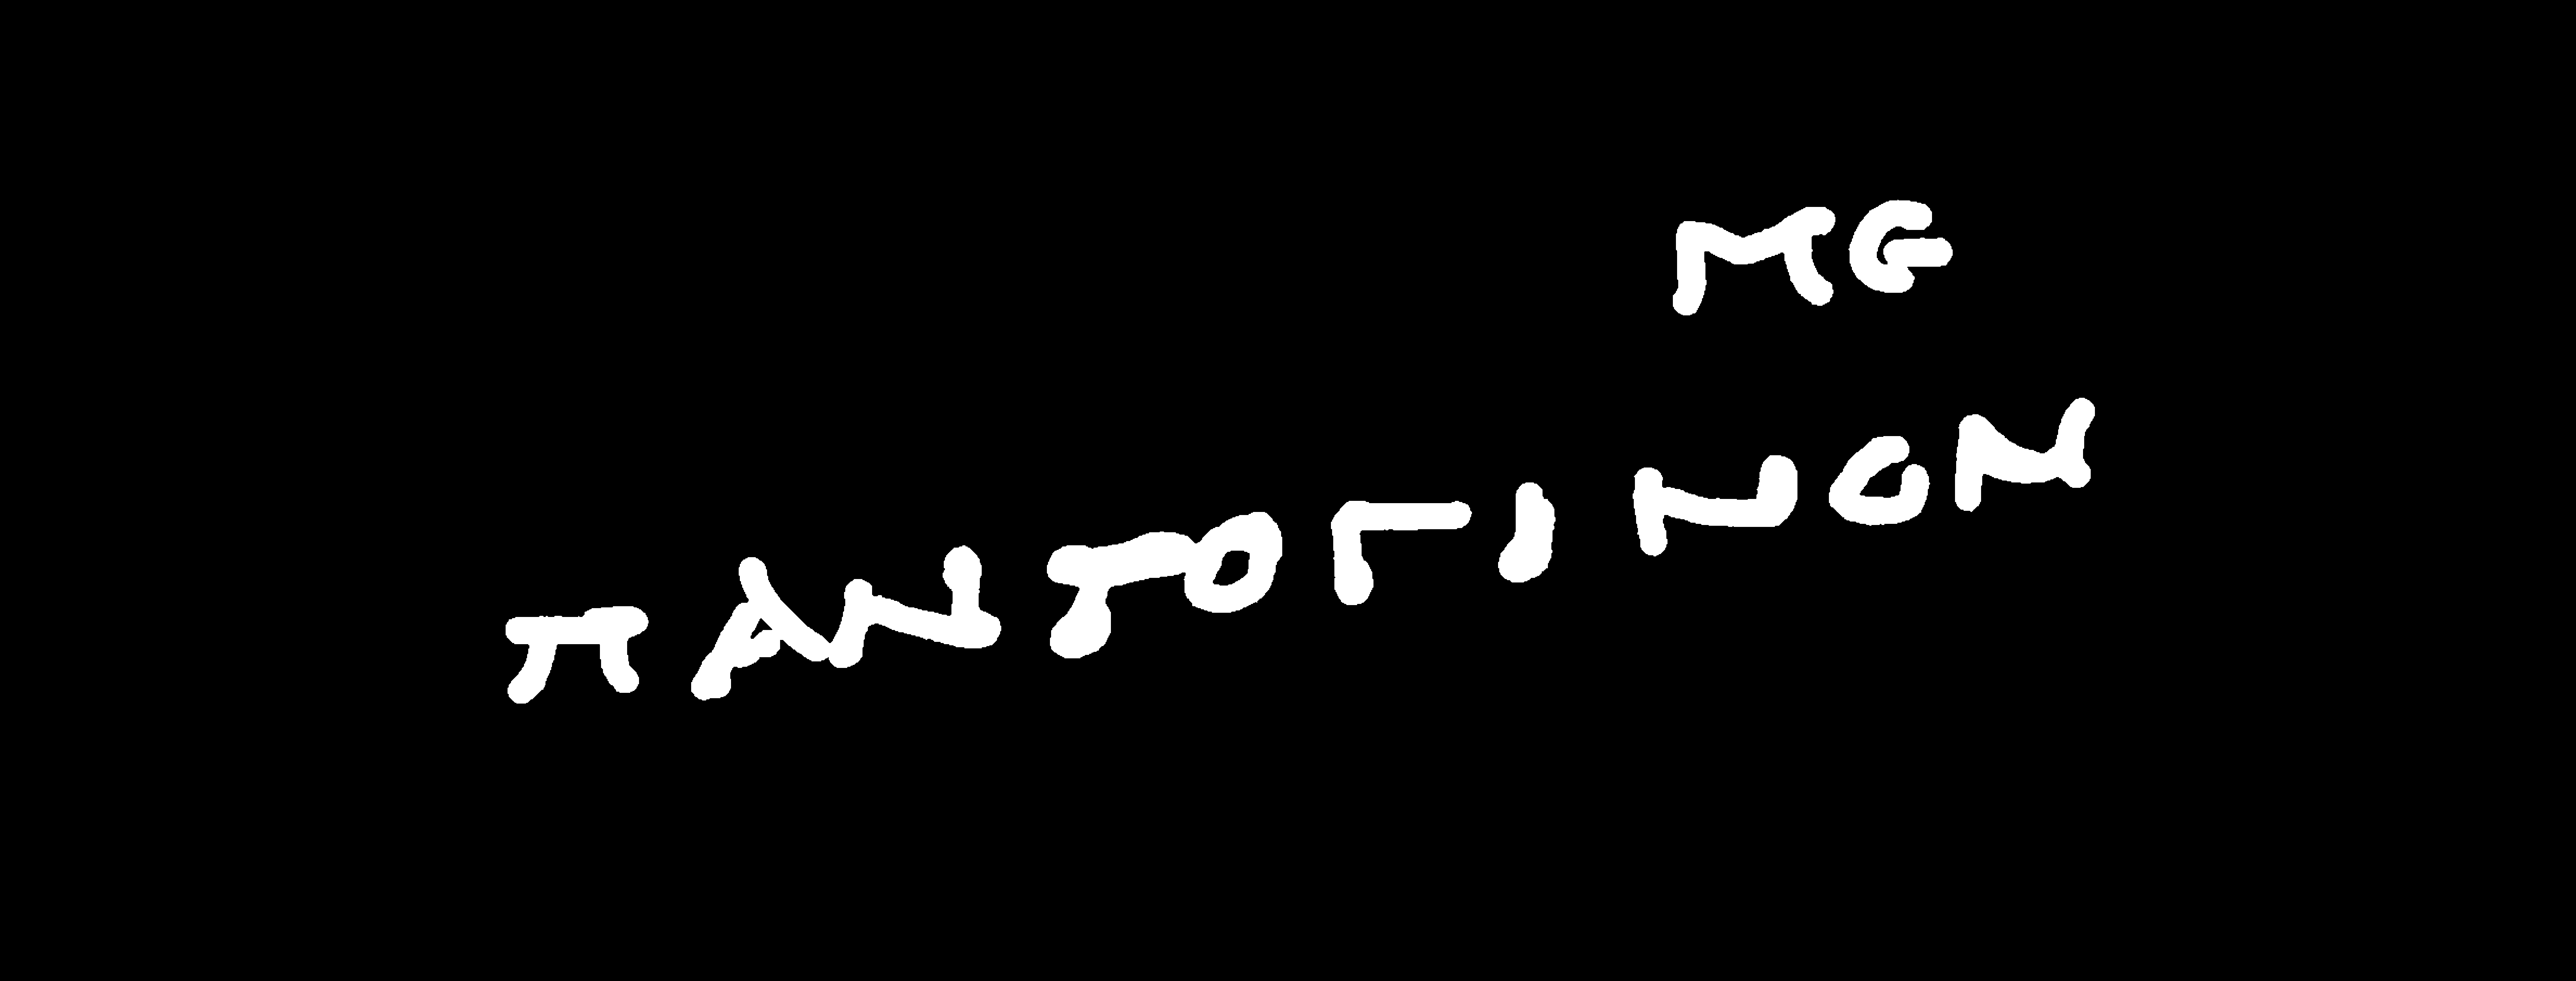
\includegraphics[width=122.48pt]{../figures/0343/0343_2_labels.png}}\end{minipage}}
\par\vspace{4pt}
\noindent\makebox[\columnwidth][c]{\begin{minipage}[t]{122.48pt}\centering\href{https://raw.githubusercontent.com/evilaliv3/vesuvius-challenge-pipeline/main/results/db27c806-rectina/src/figures/0343/0343_3_reader-v2.png}{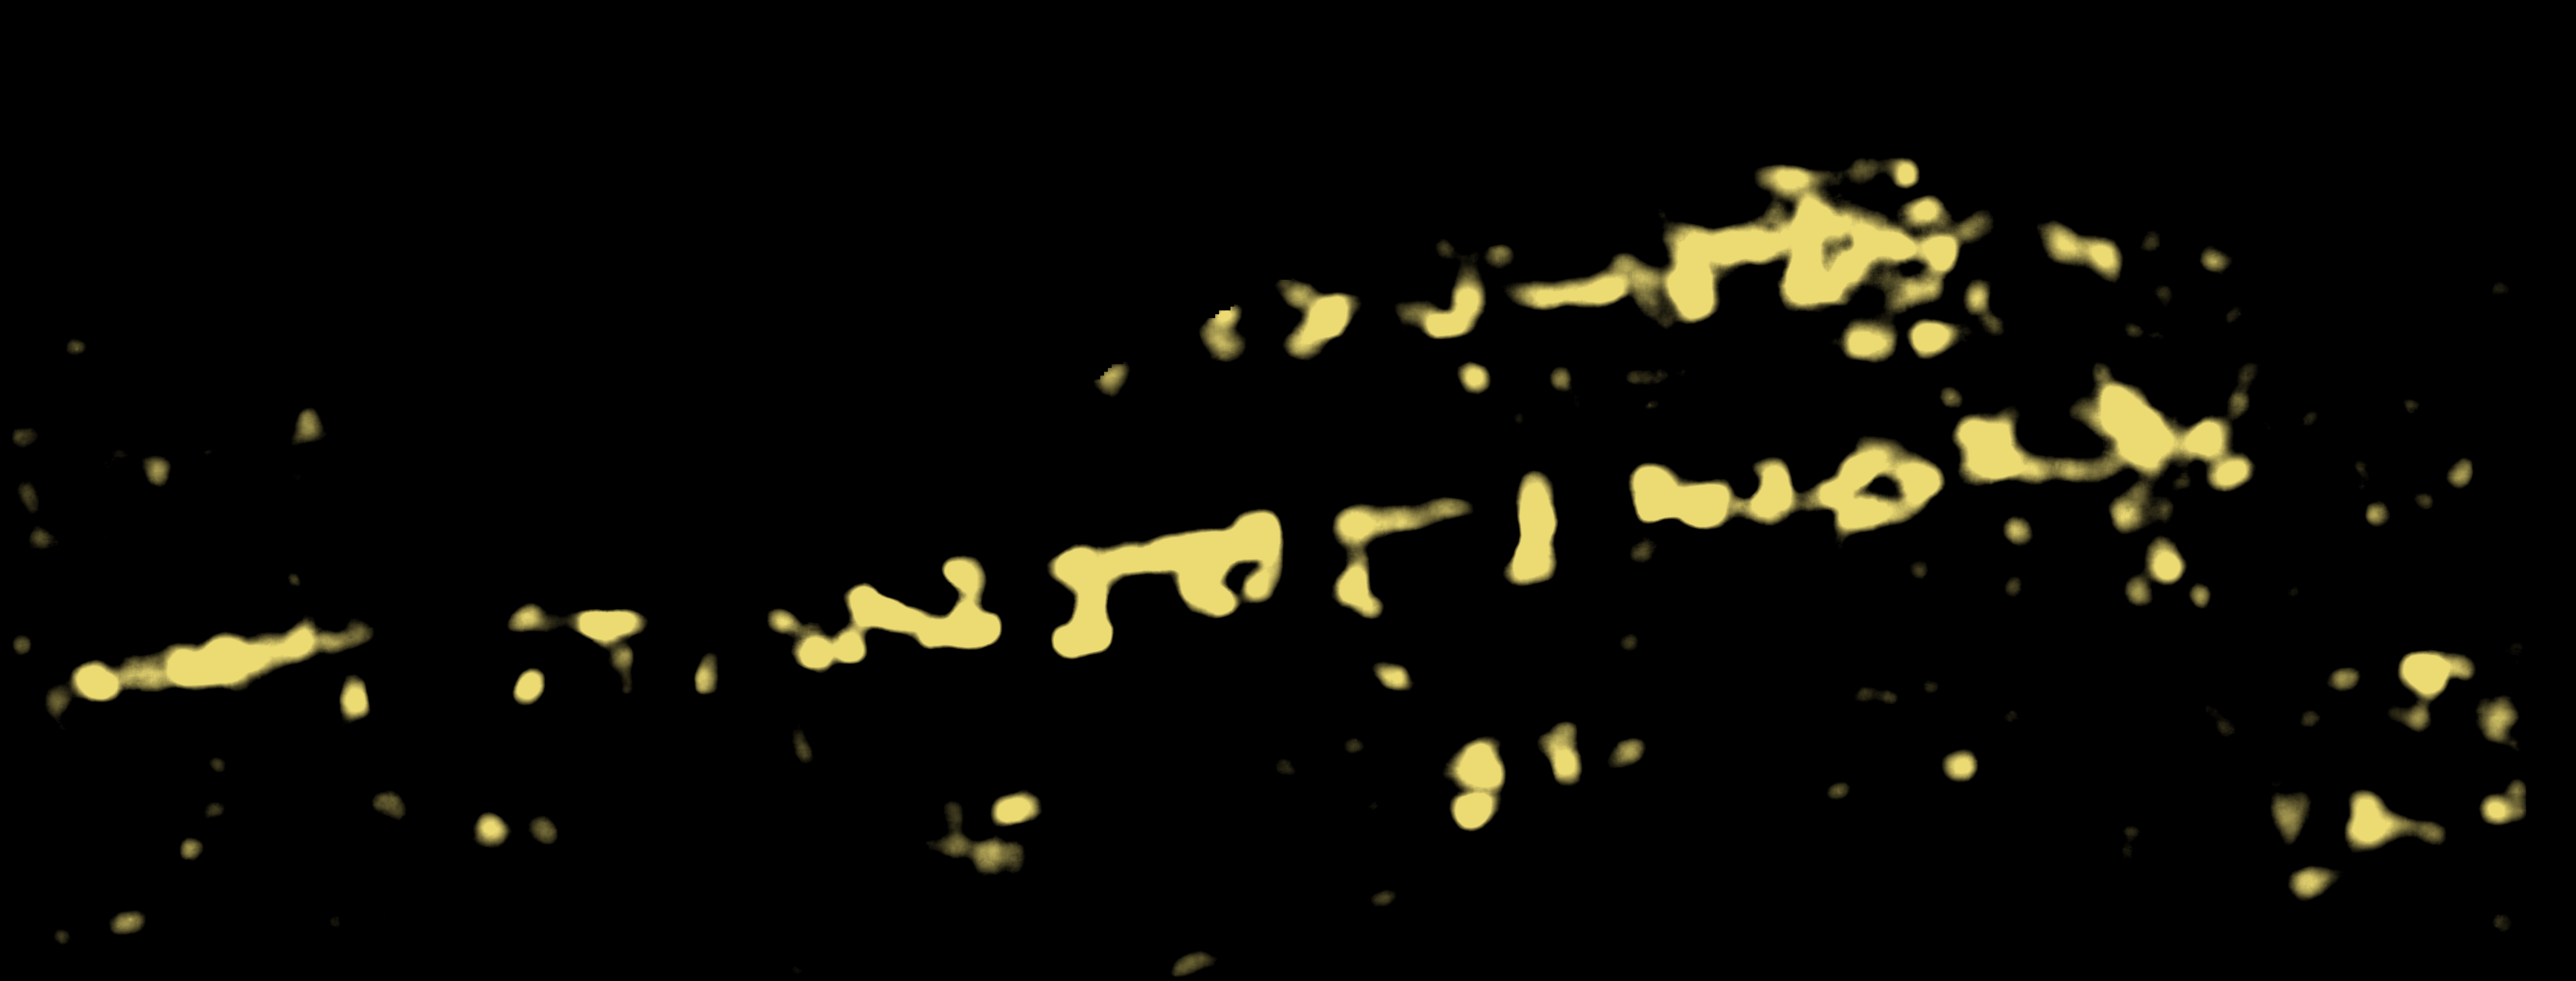
\includegraphics[width=122.48pt]{../figures/0343/0343_3_reader-v2.png}}\end{minipage}\hspace{2pt}\begin{minipage}[t]{122.48pt}\centering\href{https://raw.githubusercontent.com/evilaliv3/vesuvius-challenge-pipeline/main/results/db27c806-rectina/src/figures/0343/0343_5_rectina-m1.png}{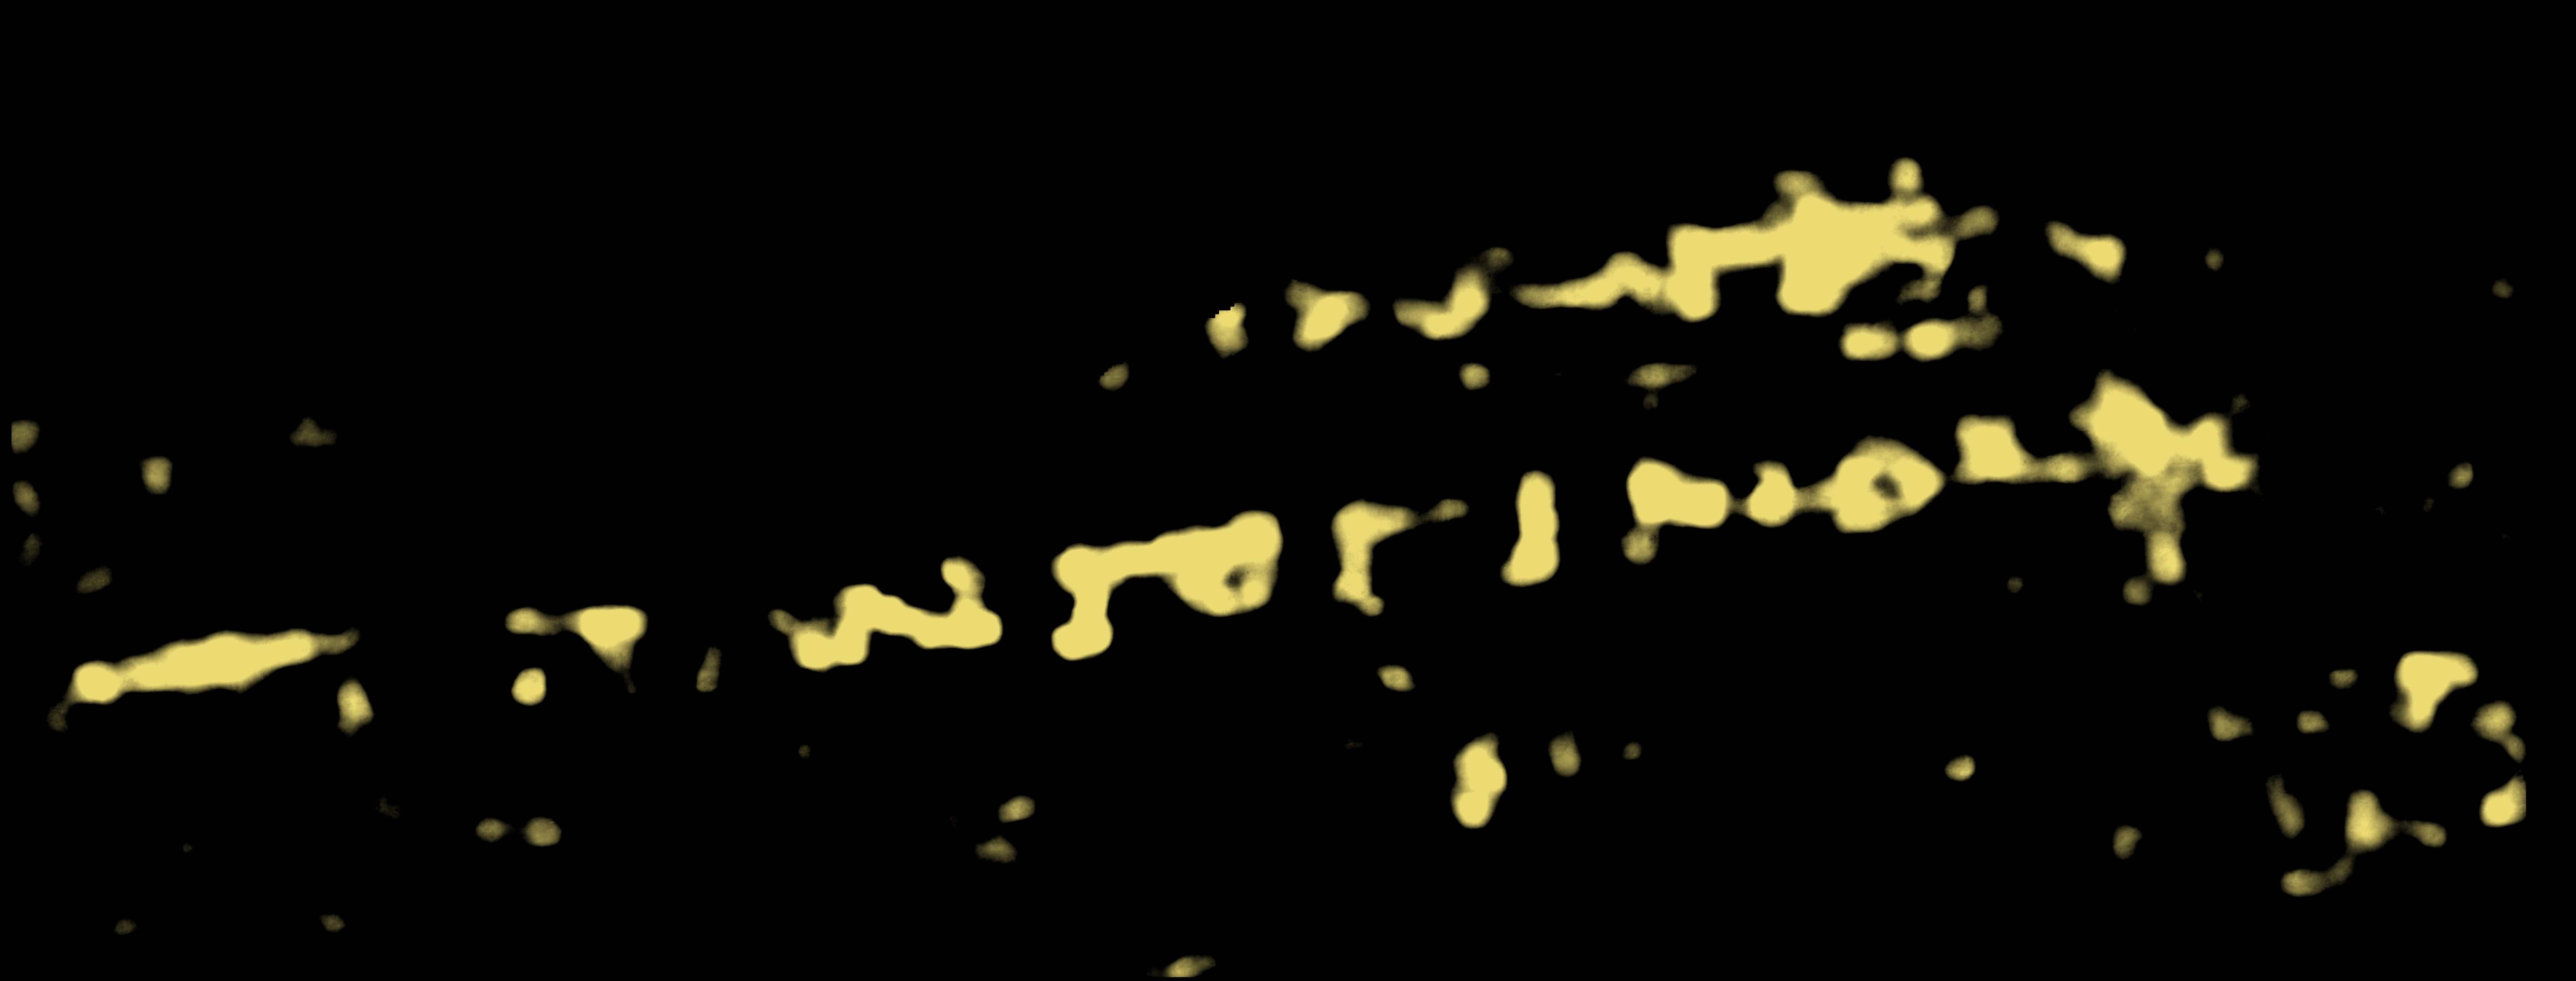
\includegraphics[width=122.48pt]{../figures/0343/0343_5_rectina-m1.png}}\end{minipage}}
\par\vspace{4pt}
\noindent\makebox[\columnwidth][c]{\begin{minipage}[t]{122.48pt}\centering\href{https://raw.githubusercontent.com/evilaliv3/vesuvius-challenge-pipeline/main/results/db27c806-rectina/src/figures/0343/0343_4_reader-v3.png}{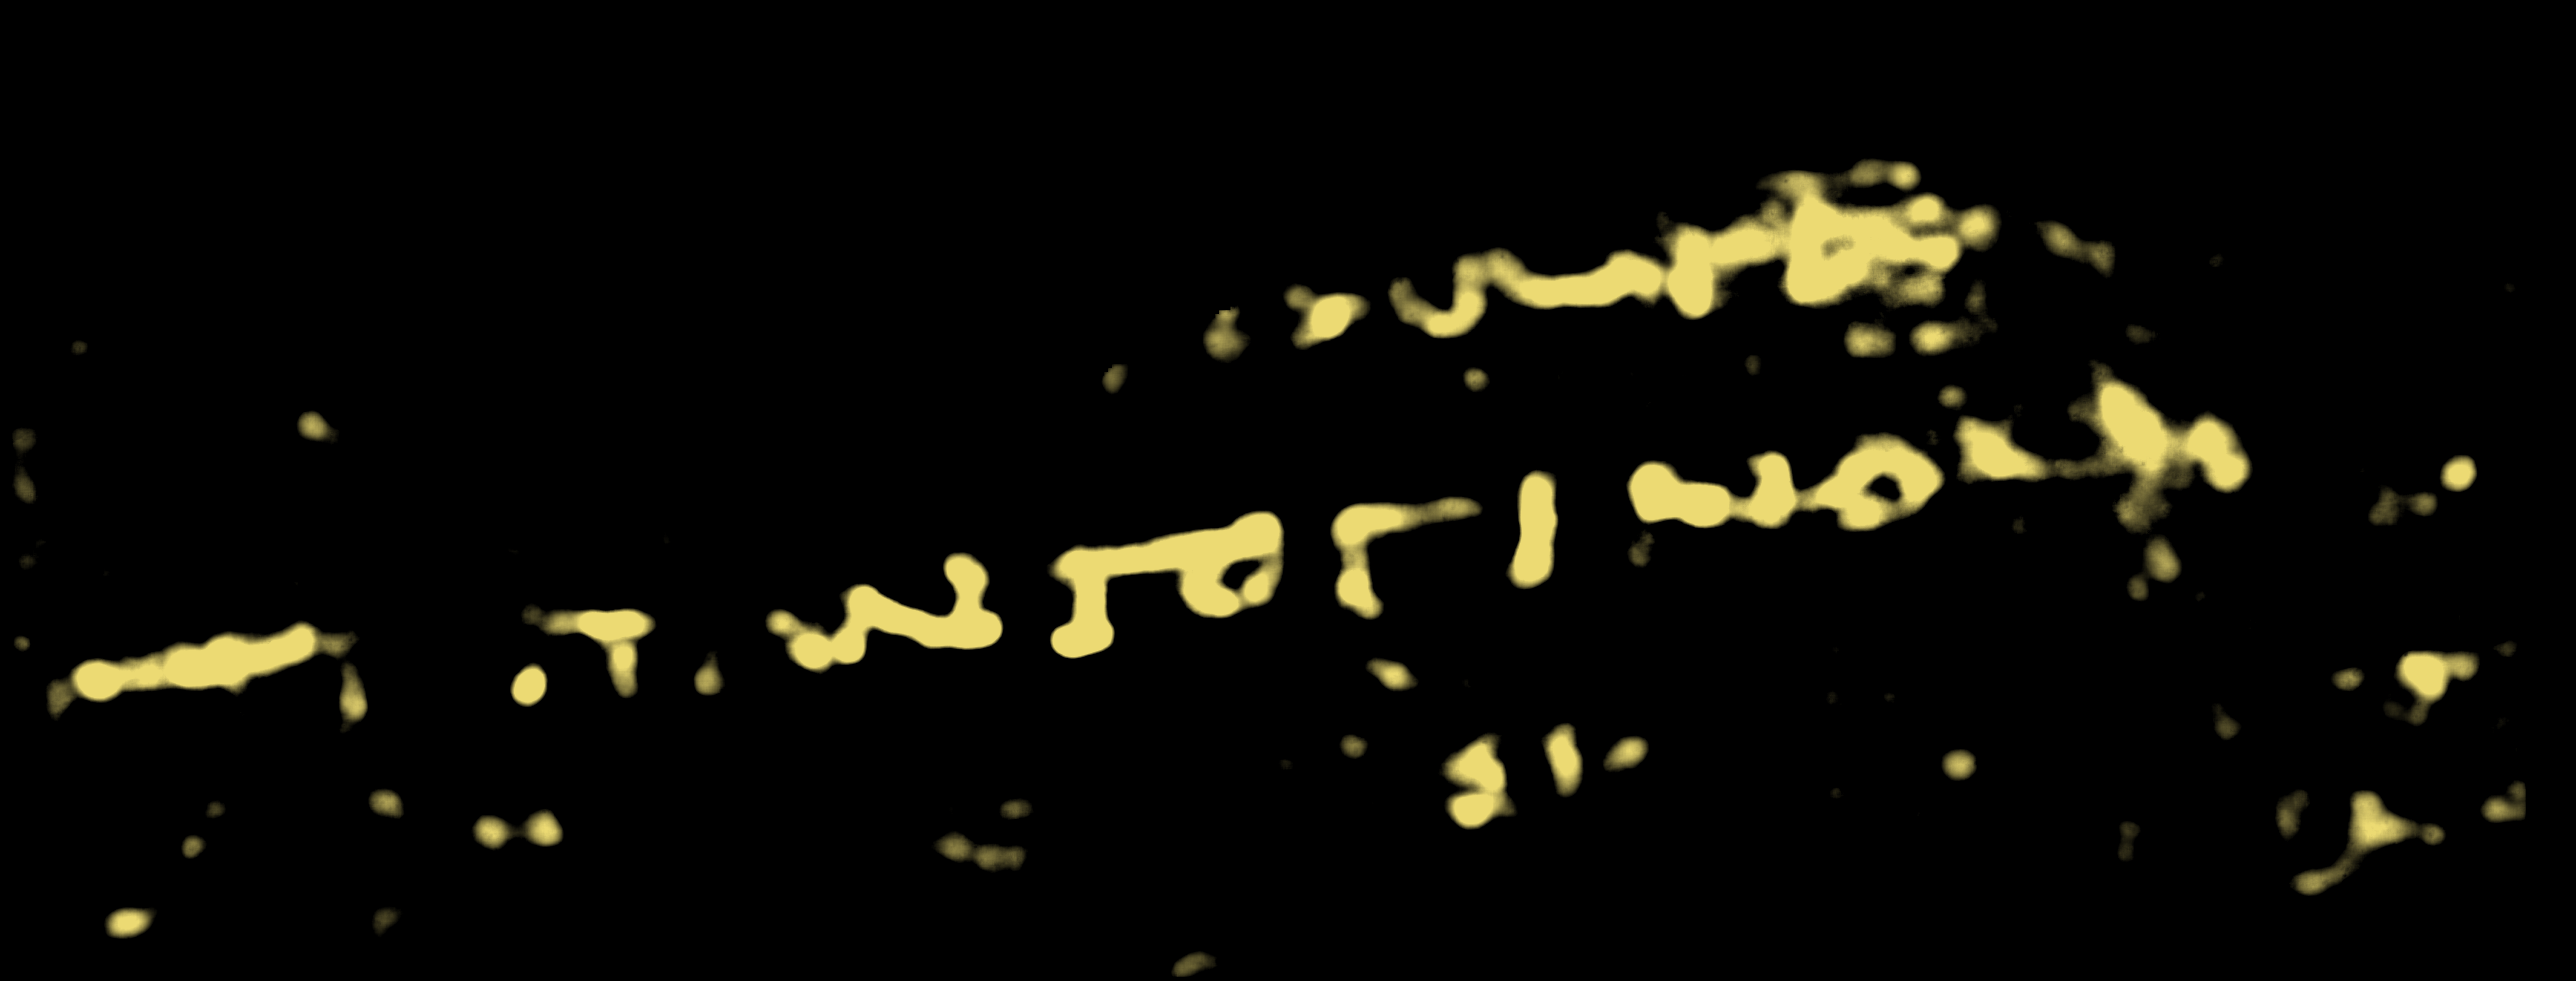
\includegraphics[width=122.48pt]{../figures/0343/0343_4_reader-v3.png}}\end{minipage}\hspace{2pt}\begin{minipage}[t]{122.48pt}\centering\href{https://raw.githubusercontent.com/evilaliv3/vesuvius-challenge-pipeline/main/results/db27c806-rectina/src/figures/0343/0343_6_rectina-m2.png}{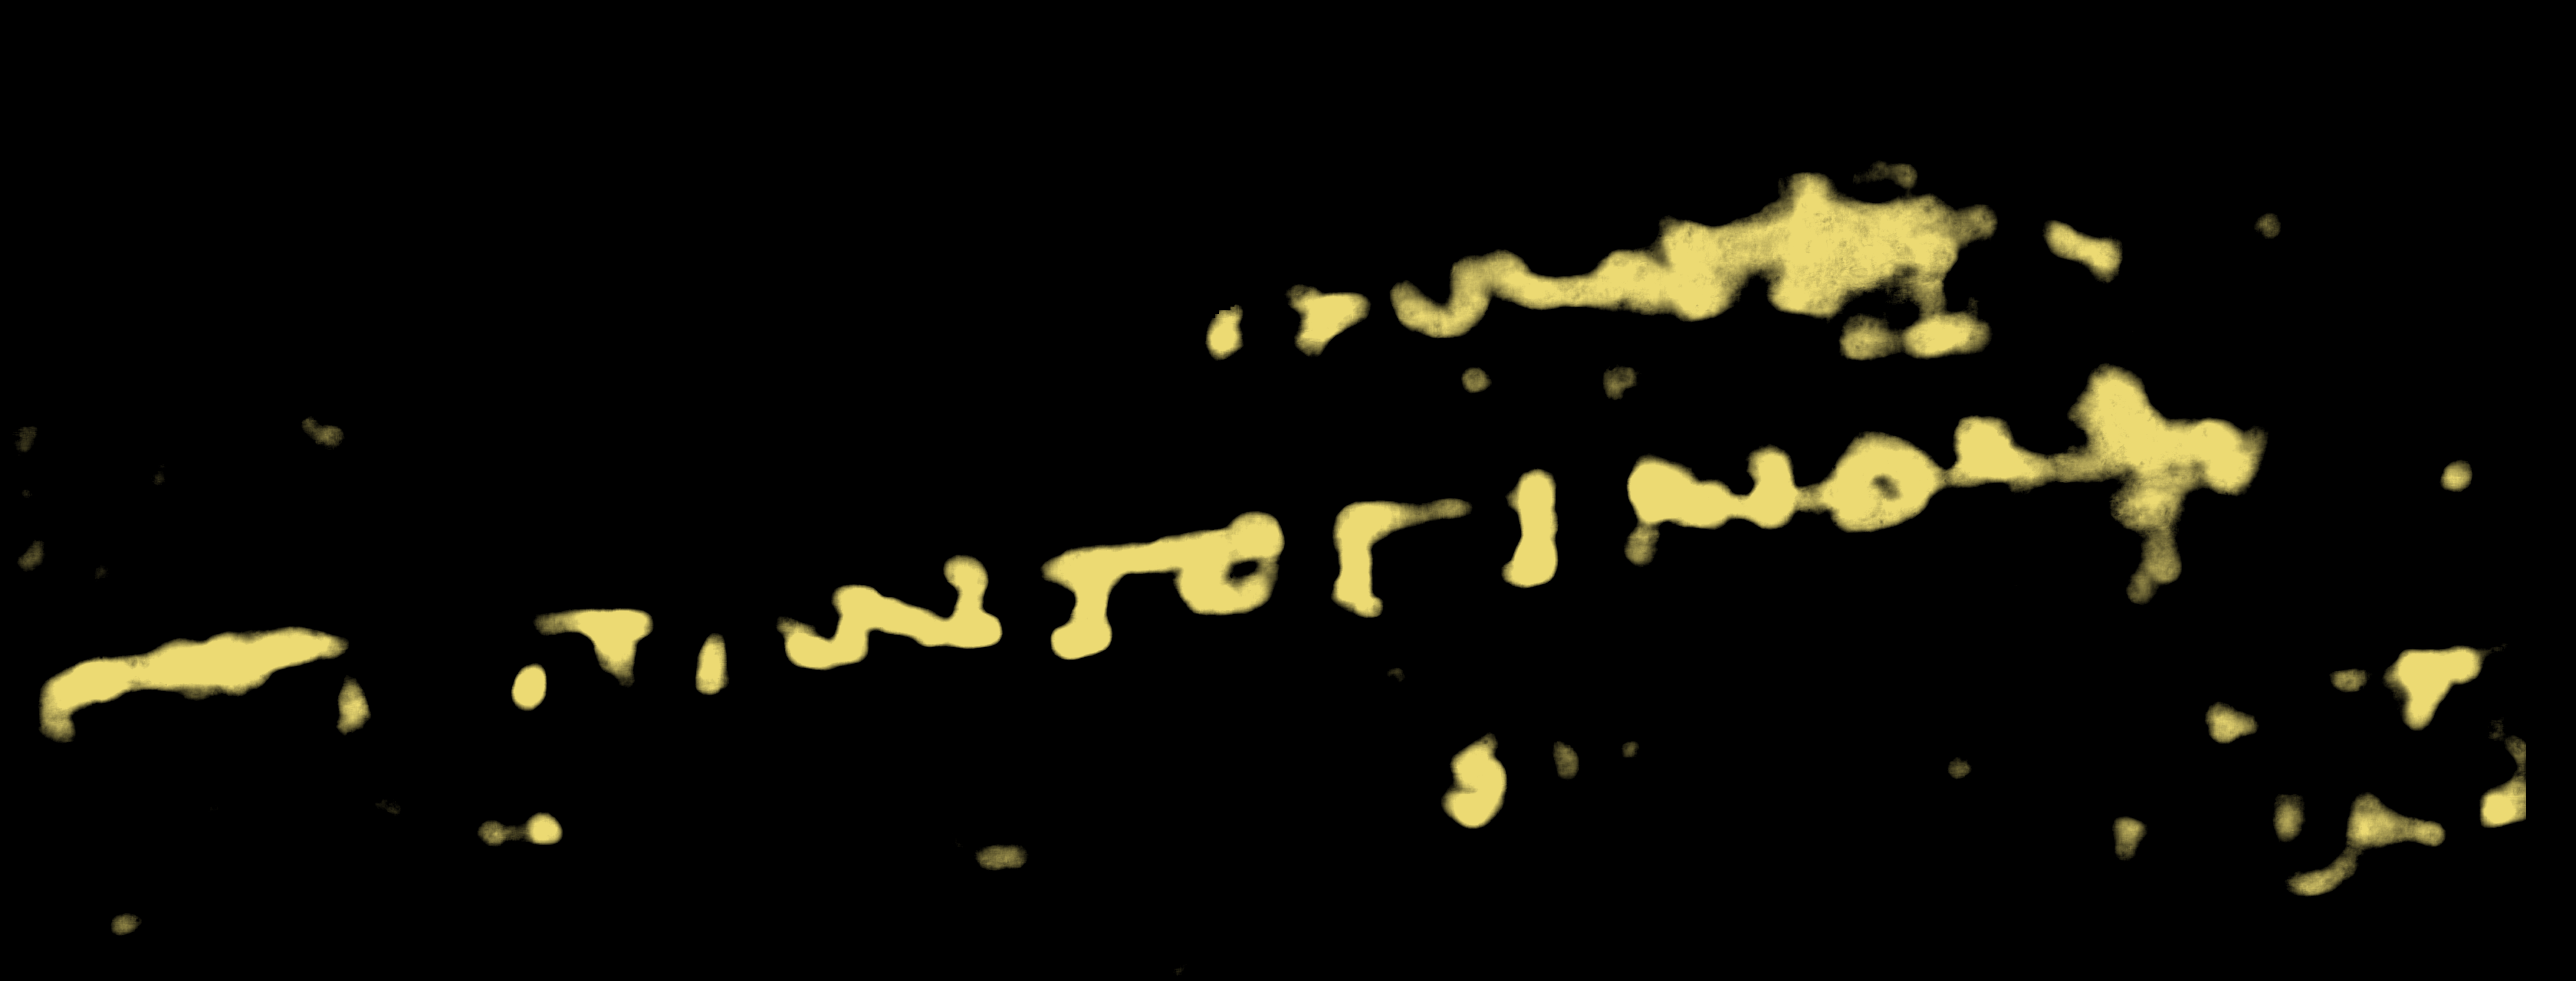
\includegraphics[width=122.48pt]{../figures/0343/0343_6_rectina-m2.png}}\end{minipage}}
\caption{Control unit 0343, three rows of two panels. Row 1: left, Texture; right, Labels. Row 2: left, Reader v2; right, Rectina m1 (display windows: Reader v2 0.409836 to 0.590749 (ramp); Rectina m1 0.548366 to 0.721975 (ramp)). Row 3: left, Reader v3; right, Rectina m2 (display windows: Reader v3 0.444697 to 0.678368 (ramp); Rectina m2 0.627931 to 0.765628 (ramp)). Each map is stretched between its own percentiles. The control is shown rotated 180 degrees, as the index of the panels records. Reader and model stand side by side in the rows 2 and 3.}
\end{figure}

\begin{figure}[!tbp]
\centering
\noindent\makebox[\columnwidth][c]{\begin{minipage}[t]{122.48pt}\centering\href{https://raw.githubusercontent.com/evilaliv3/vesuvius-challenge-pipeline/main/results/db27c806-rectina/src/figures/w058/w058_1_texture.png}{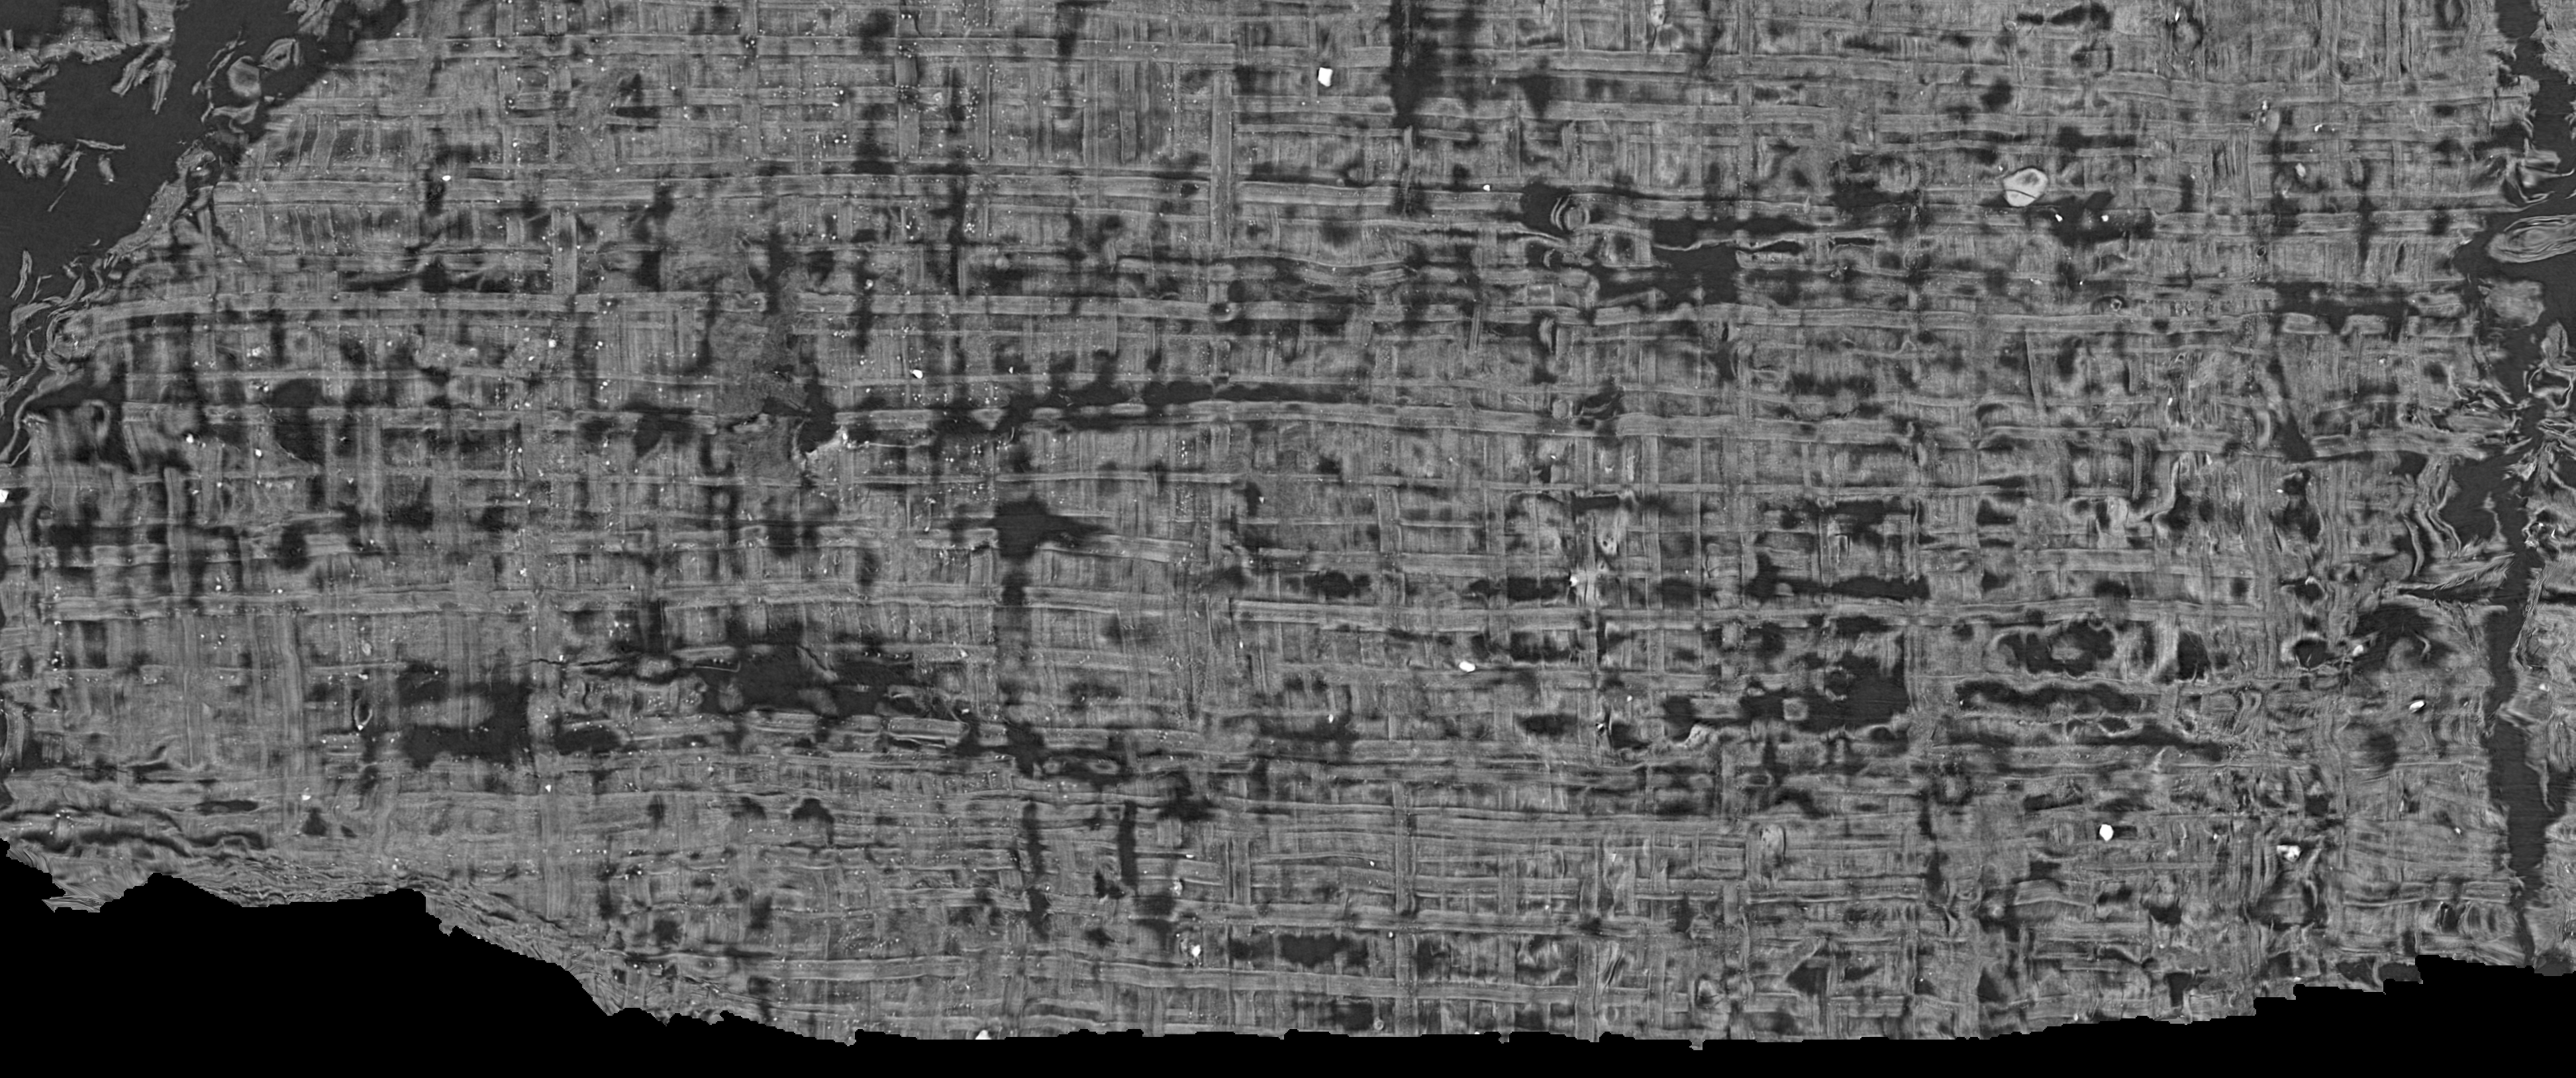
\includegraphics[width=122.48pt]{../figures/w058/w058_1_texture.png}}\end{minipage}\hspace{2pt}\begin{minipage}[t]{122.48pt}\centering\href{https://raw.githubusercontent.com/evilaliv3/vesuvius-challenge-pipeline/main/results/db27c806-rectina/src/figures/w058/w058_2_labels.png}{
\includegraphics[width=122.48pt]{../figures/w058/w058_2_labels.png}}\end{minipage}}
\par\vspace{4pt}
\noindent\makebox[\columnwidth][c]{\begin{minipage}[t]{122.48pt}\centering\href{https://raw.githubusercontent.com/evilaliv3/vesuvius-challenge-pipeline/main/results/db27c806-rectina/src/figures/w058/w058_3_reader-v2.png}{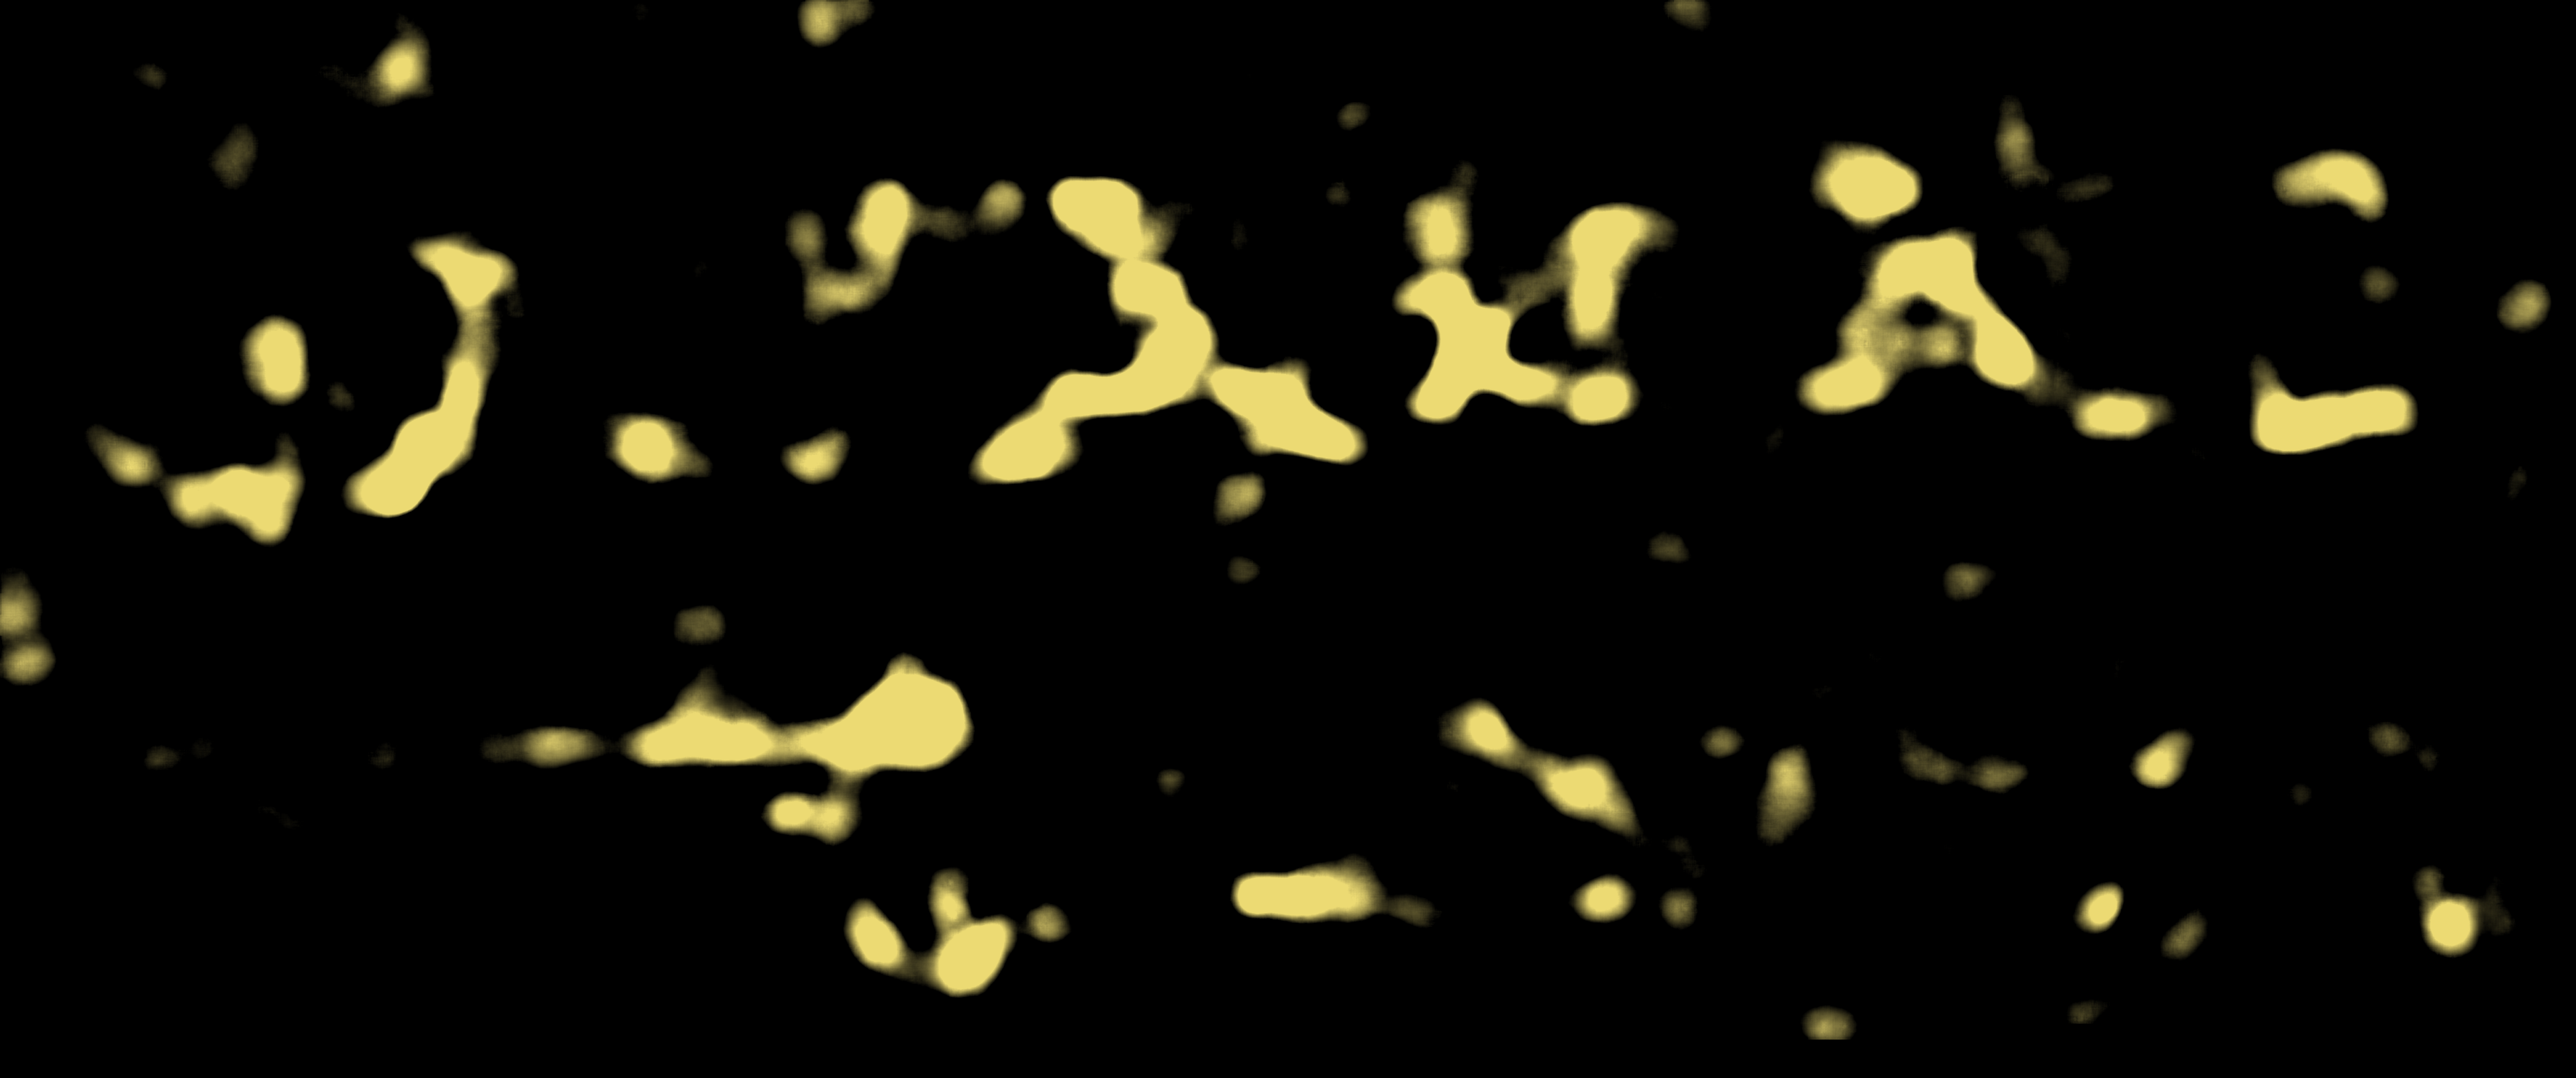
\includegraphics[width=122.48pt]{../figures/w058/w058_3_reader-v2.png}}\end{minipage}\hspace{2pt}\begin{minipage}[t]{122.48pt}\centering\href{https://raw.githubusercontent.com/evilaliv3/vesuvius-challenge-pipeline/main/results/db27c806-rectina/src/figures/w058/w058_5_rectina-m1.png}{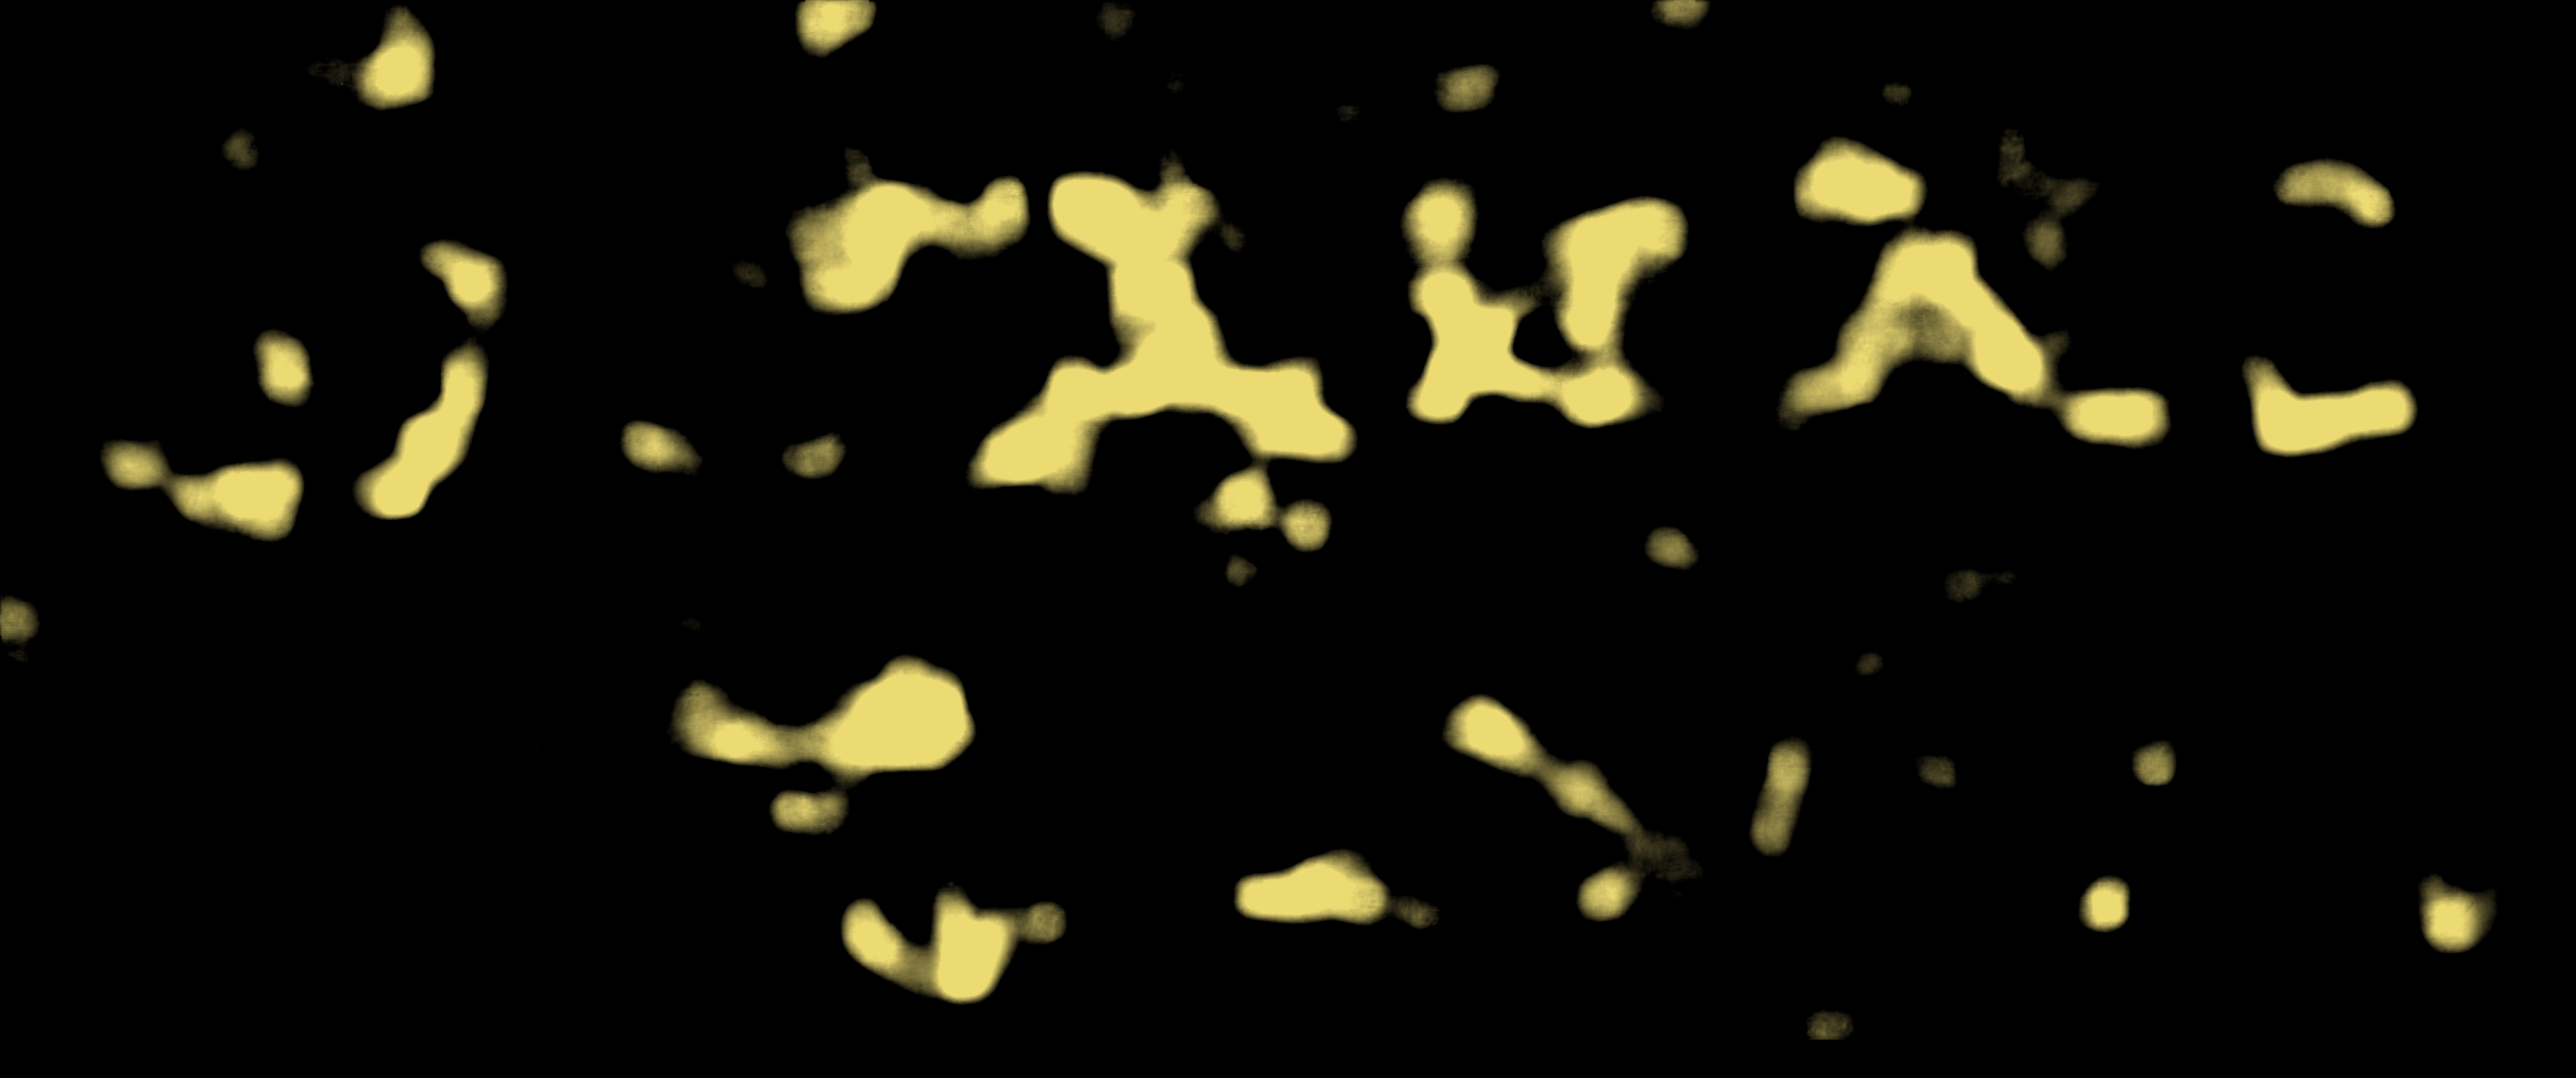
\includegraphics[width=122.48pt]{../figures/w058/w058_5_rectina-m1.png}}\end{minipage}}
\par\vspace{4pt}
\noindent\makebox[\columnwidth][c]{\begin{minipage}[t]{122.48pt}\centering\href{https://raw.githubusercontent.com/evilaliv3/vesuvius-challenge-pipeline/main/results/db27c806-rectina/src/figures/w058/w058_4_reader-v3.png}{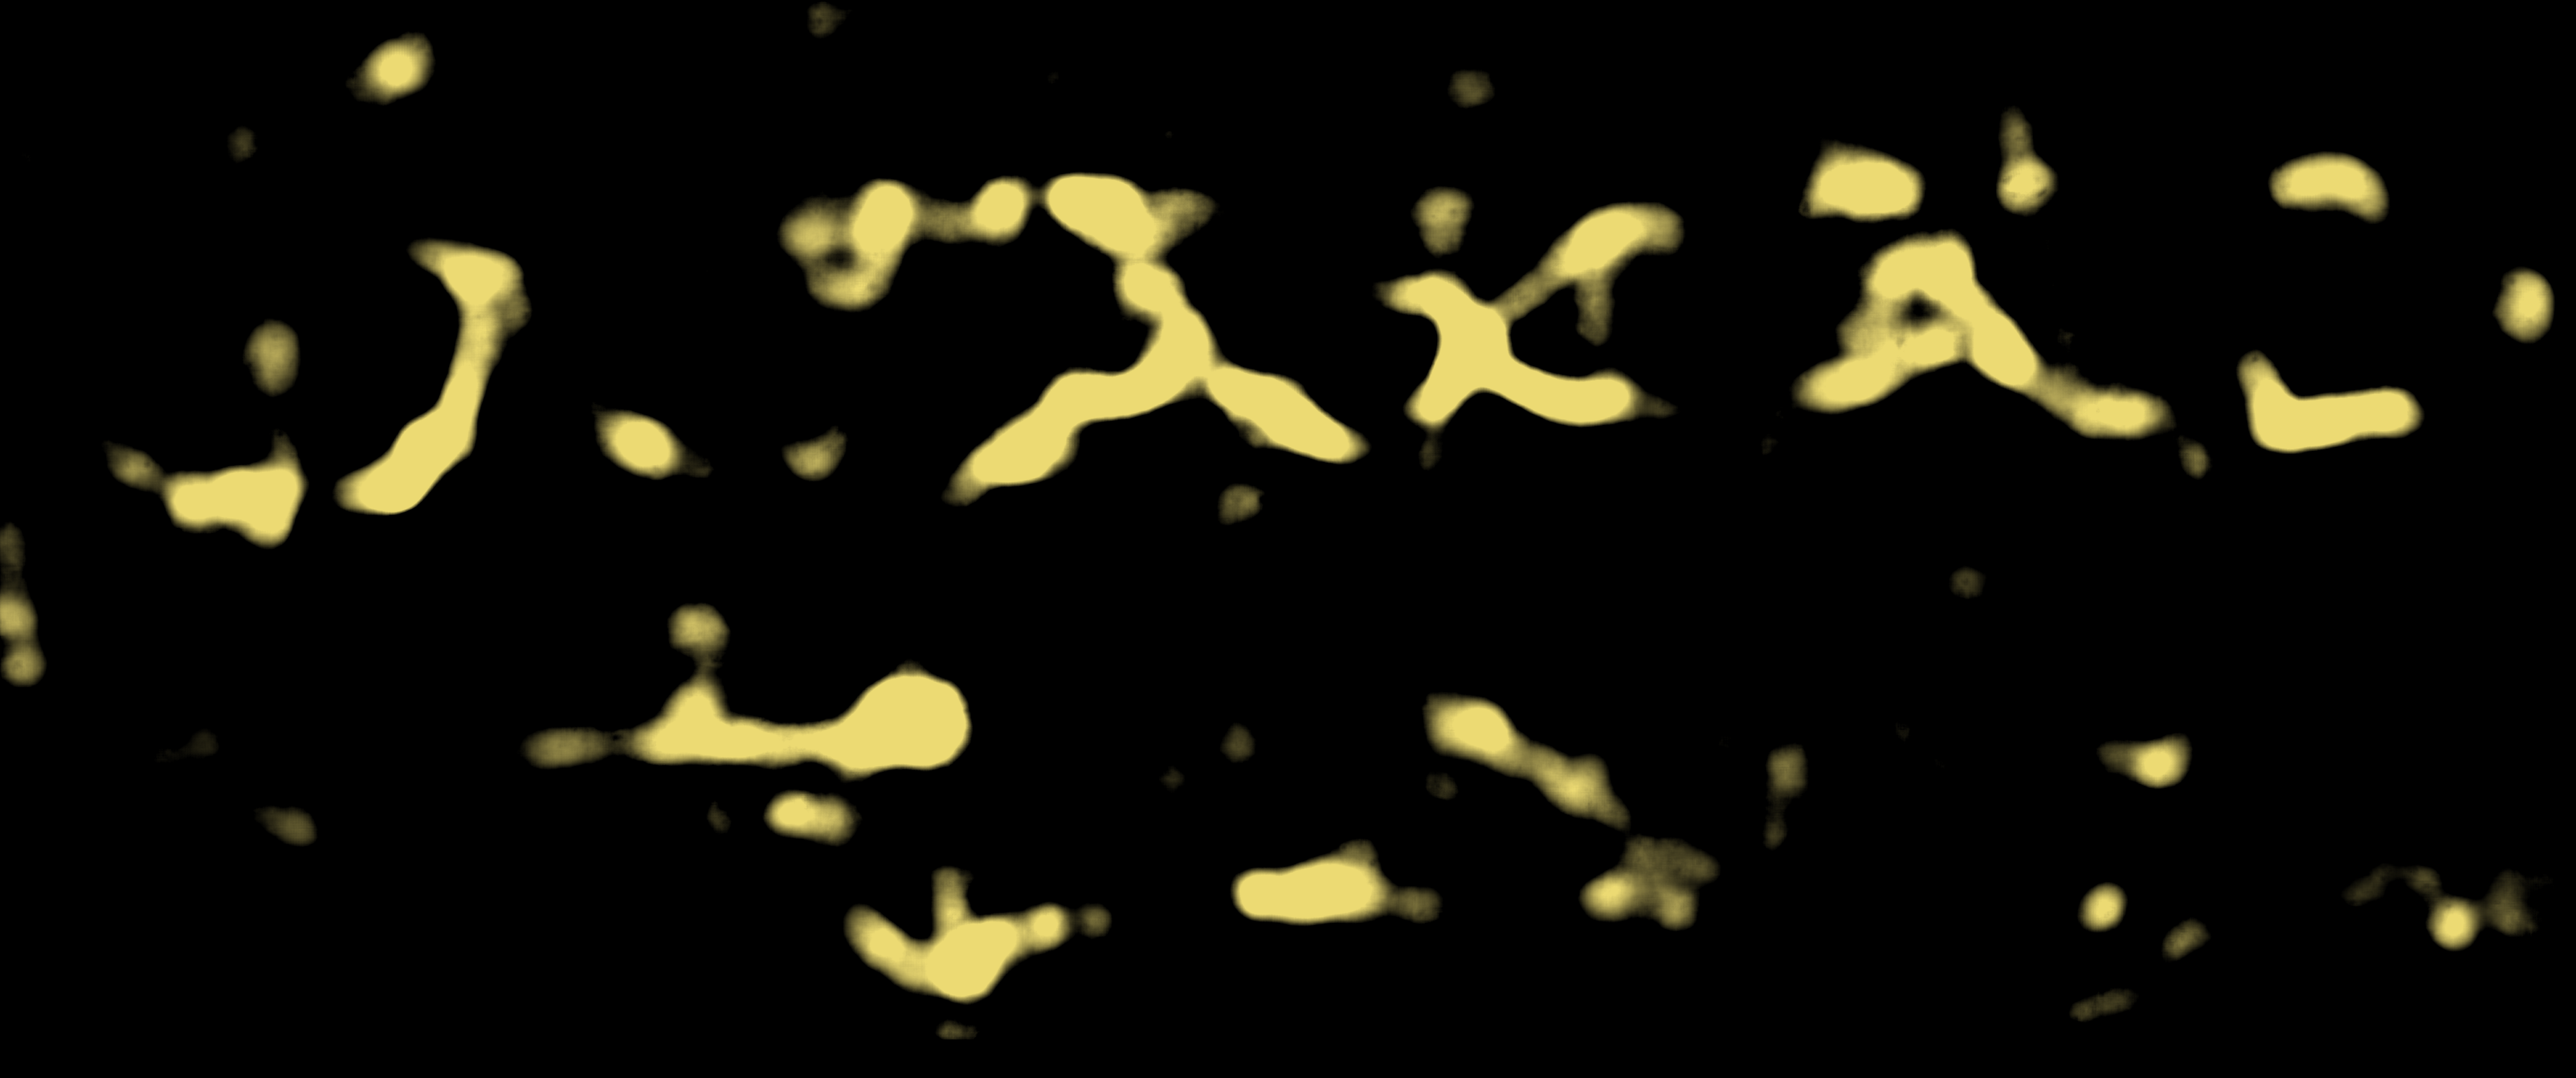
\includegraphics[width=122.48pt]{../figures/w058/w058_4_reader-v3.png}}\end{minipage}\hspace{2pt}\begin{minipage}[t]{122.48pt}\centering\href{https://raw.githubusercontent.com/evilaliv3/vesuvius-challenge-pipeline/main/results/db27c806-rectina/src/figures/w058/w058_6_rectina-m2.png}{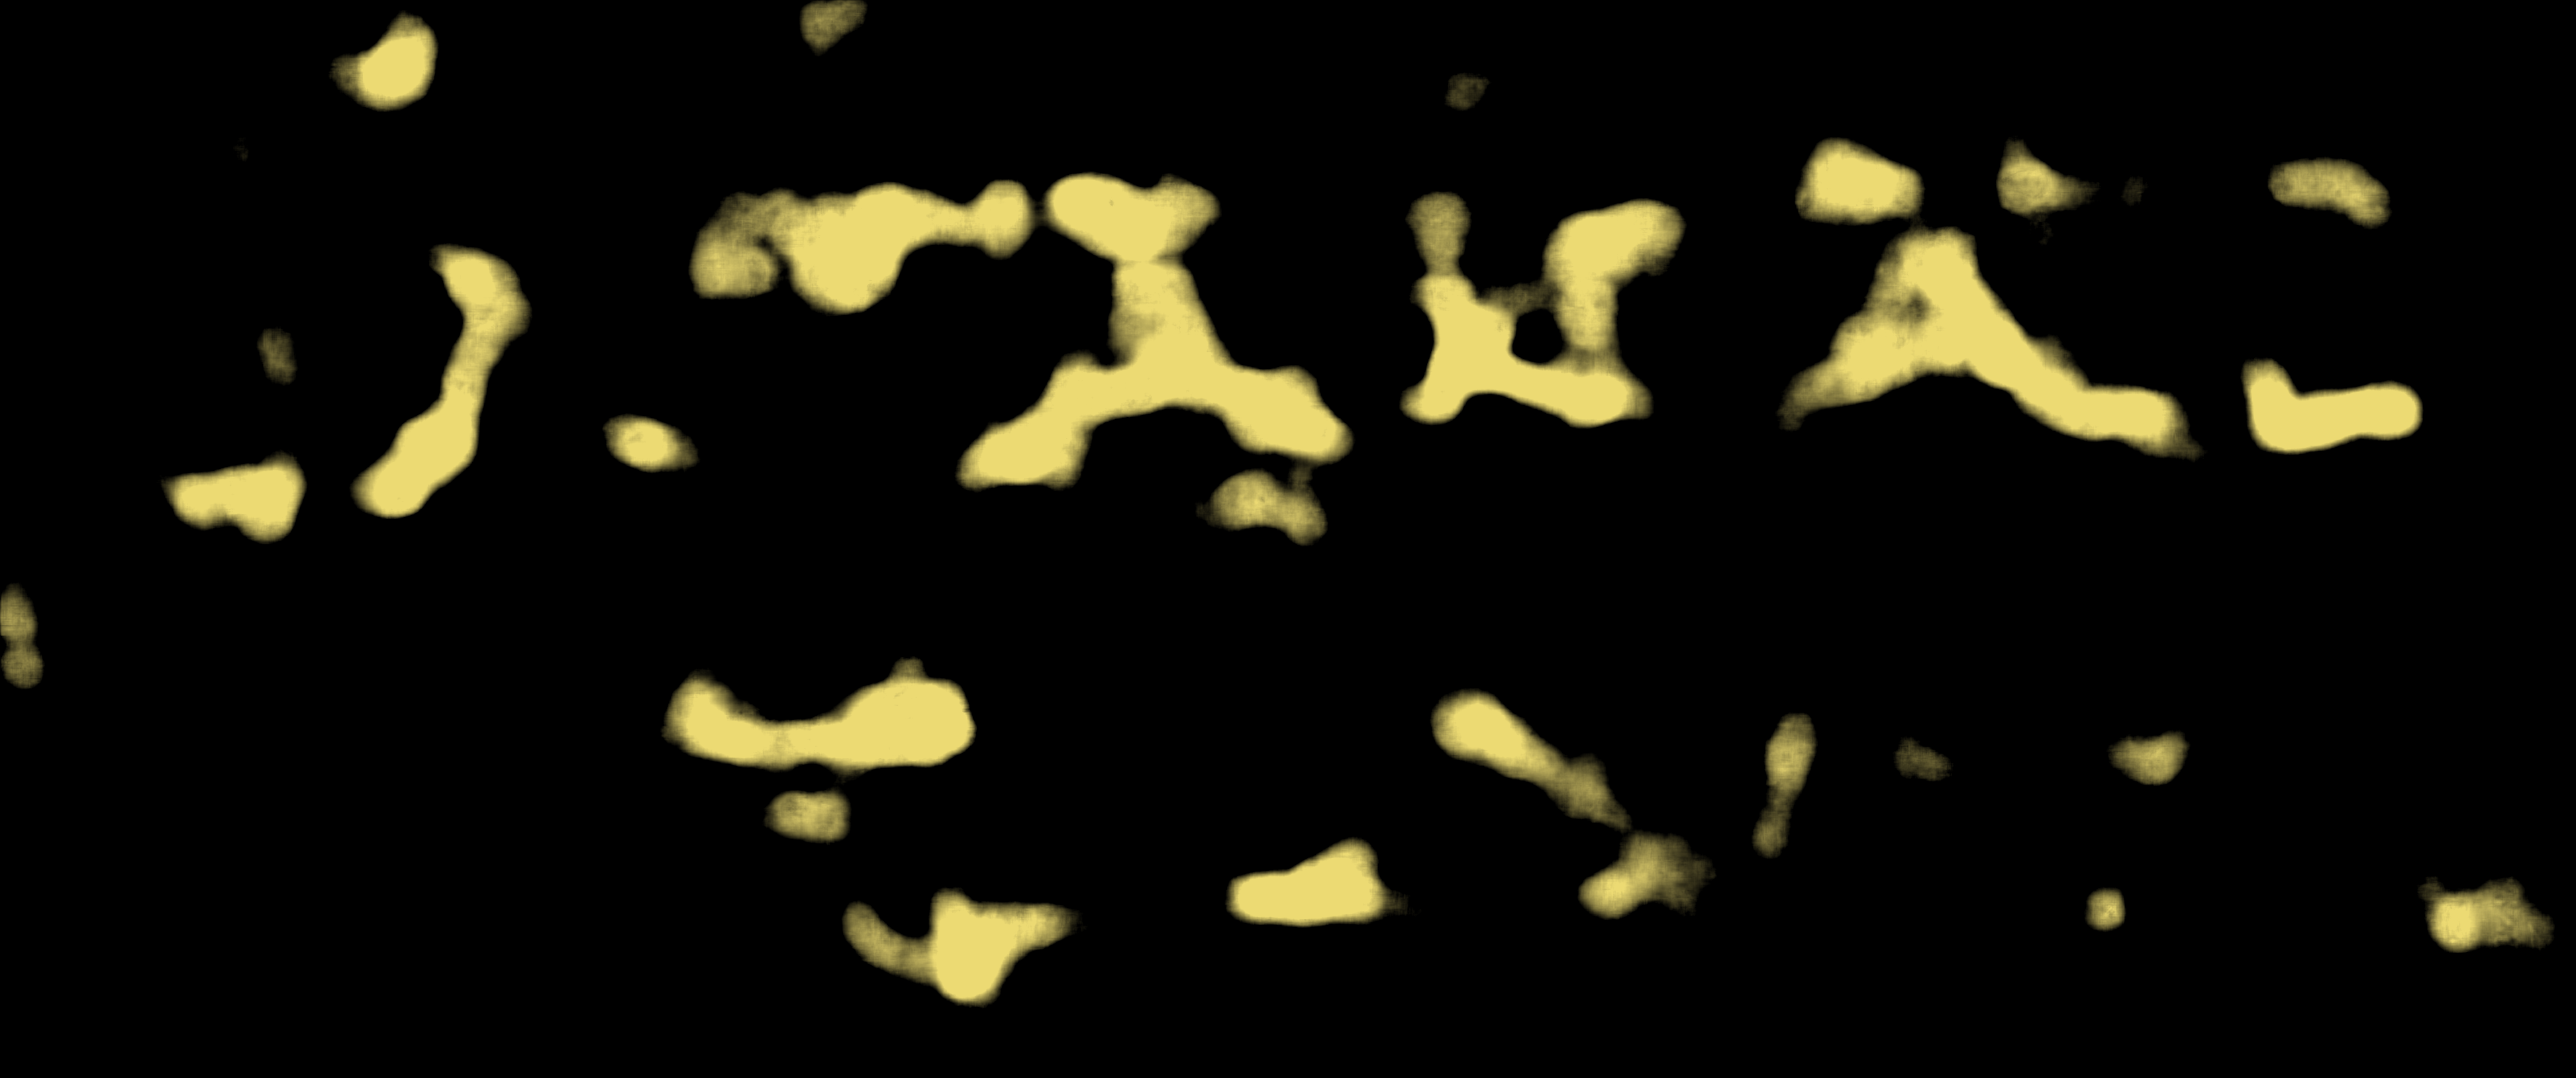
\includegraphics[width=122.48pt]{../figures/w058/w058_6_rectina-m2.png}}\end{minipage}}
\caption{Control unit 1447 w058, three rows of two panels. Row 1: left, Texture; right, Labels. Row 2: left, Reader v2; right, Rectina m1 (display windows: Reader v2 0.385394 to 0.561662 (ramp); Rectina m1 0.533701 to 0.711716 (ramp)). Row 3: left, Reader v3; right, Rectina m2 (display windows: Reader v3 0.450583 to 0.670398 (ramp); Rectina m2 0.625307 to 0.773366 (ramp)). Each map is stretched between its own percentiles. Reader and model stand side by side in the rows 2 and 3.}
\end{figure}

\begin{figure}[!tbp]
\centering
\noindent\makebox[\columnwidth][c]{\begin{minipage}[t]{122.48pt}\centering\href{https://raw.githubusercontent.com/evilaliv3/vesuvius-challenge-pipeline/main/results/db27c806-rectina/src/figures/w060/w060_1_texture.png}{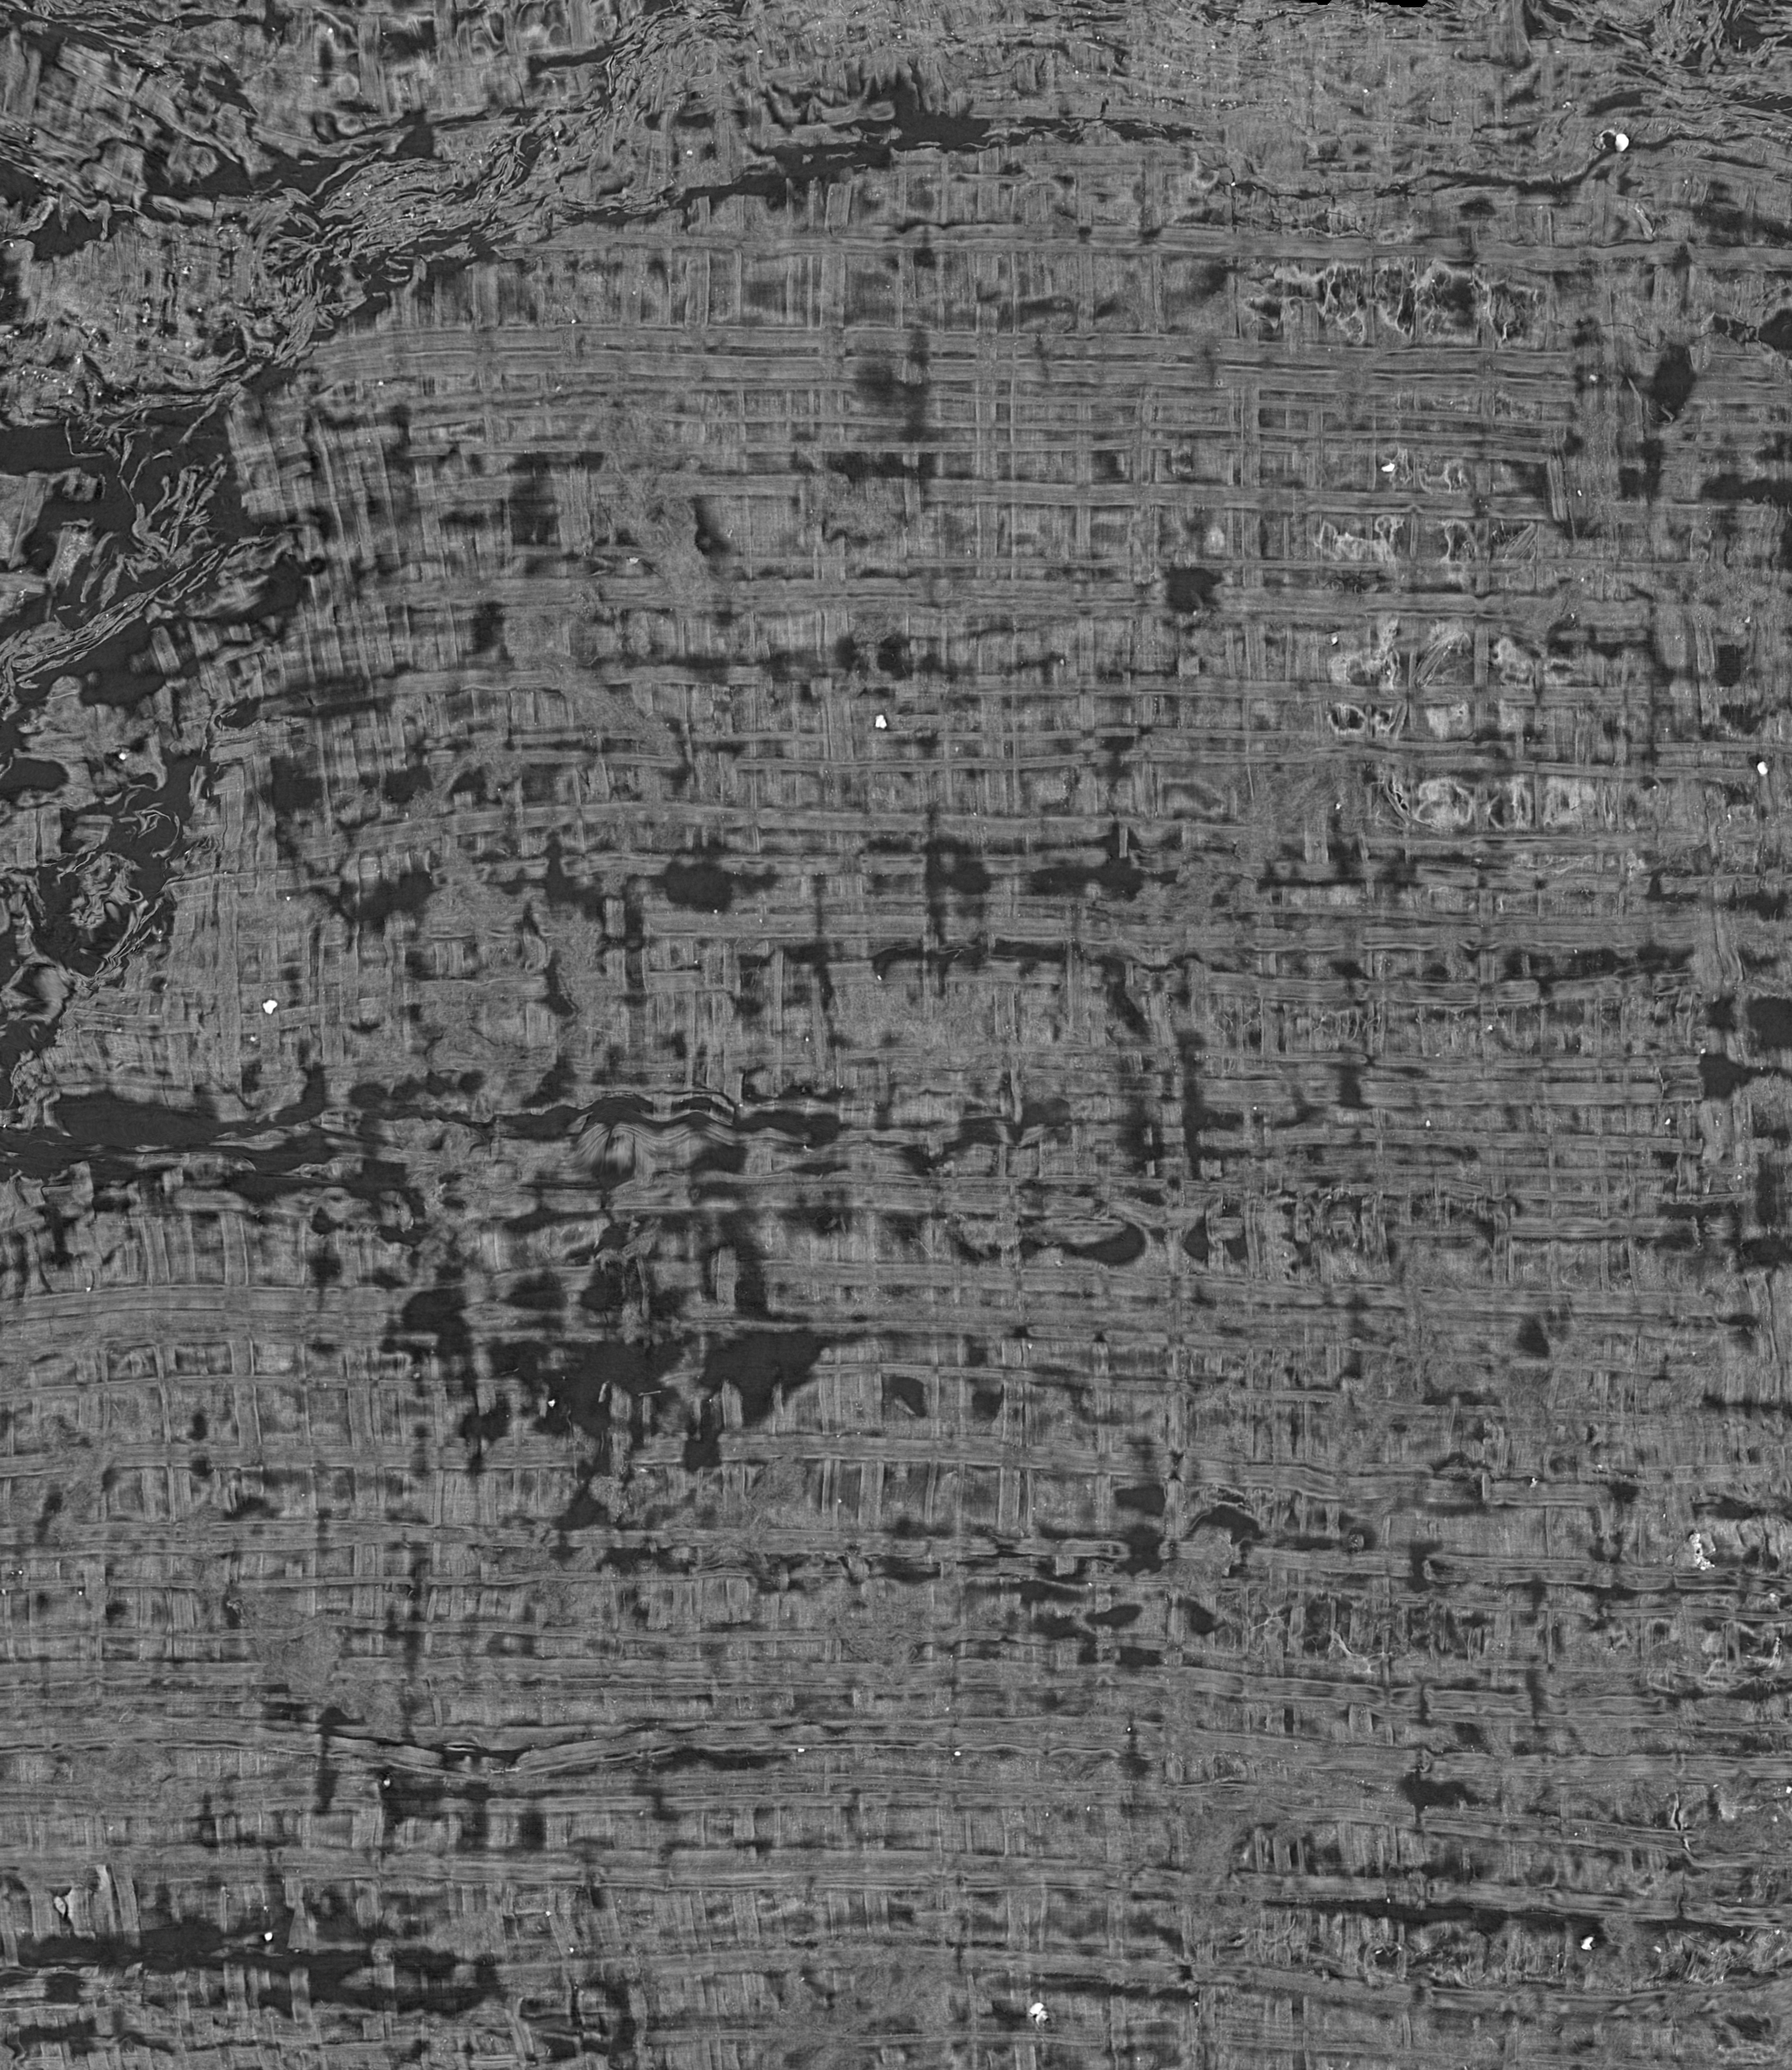
\includegraphics[width=122.48pt]{../figures/w060/w060_1_texture.png}}\end{minipage}\hspace{2pt}\begin{minipage}[t]{122.48pt}\centering\href{https://raw.githubusercontent.com/evilaliv3/vesuvius-challenge-pipeline/main/results/db27c806-rectina/src/figures/w060/w060_2_labels.png}{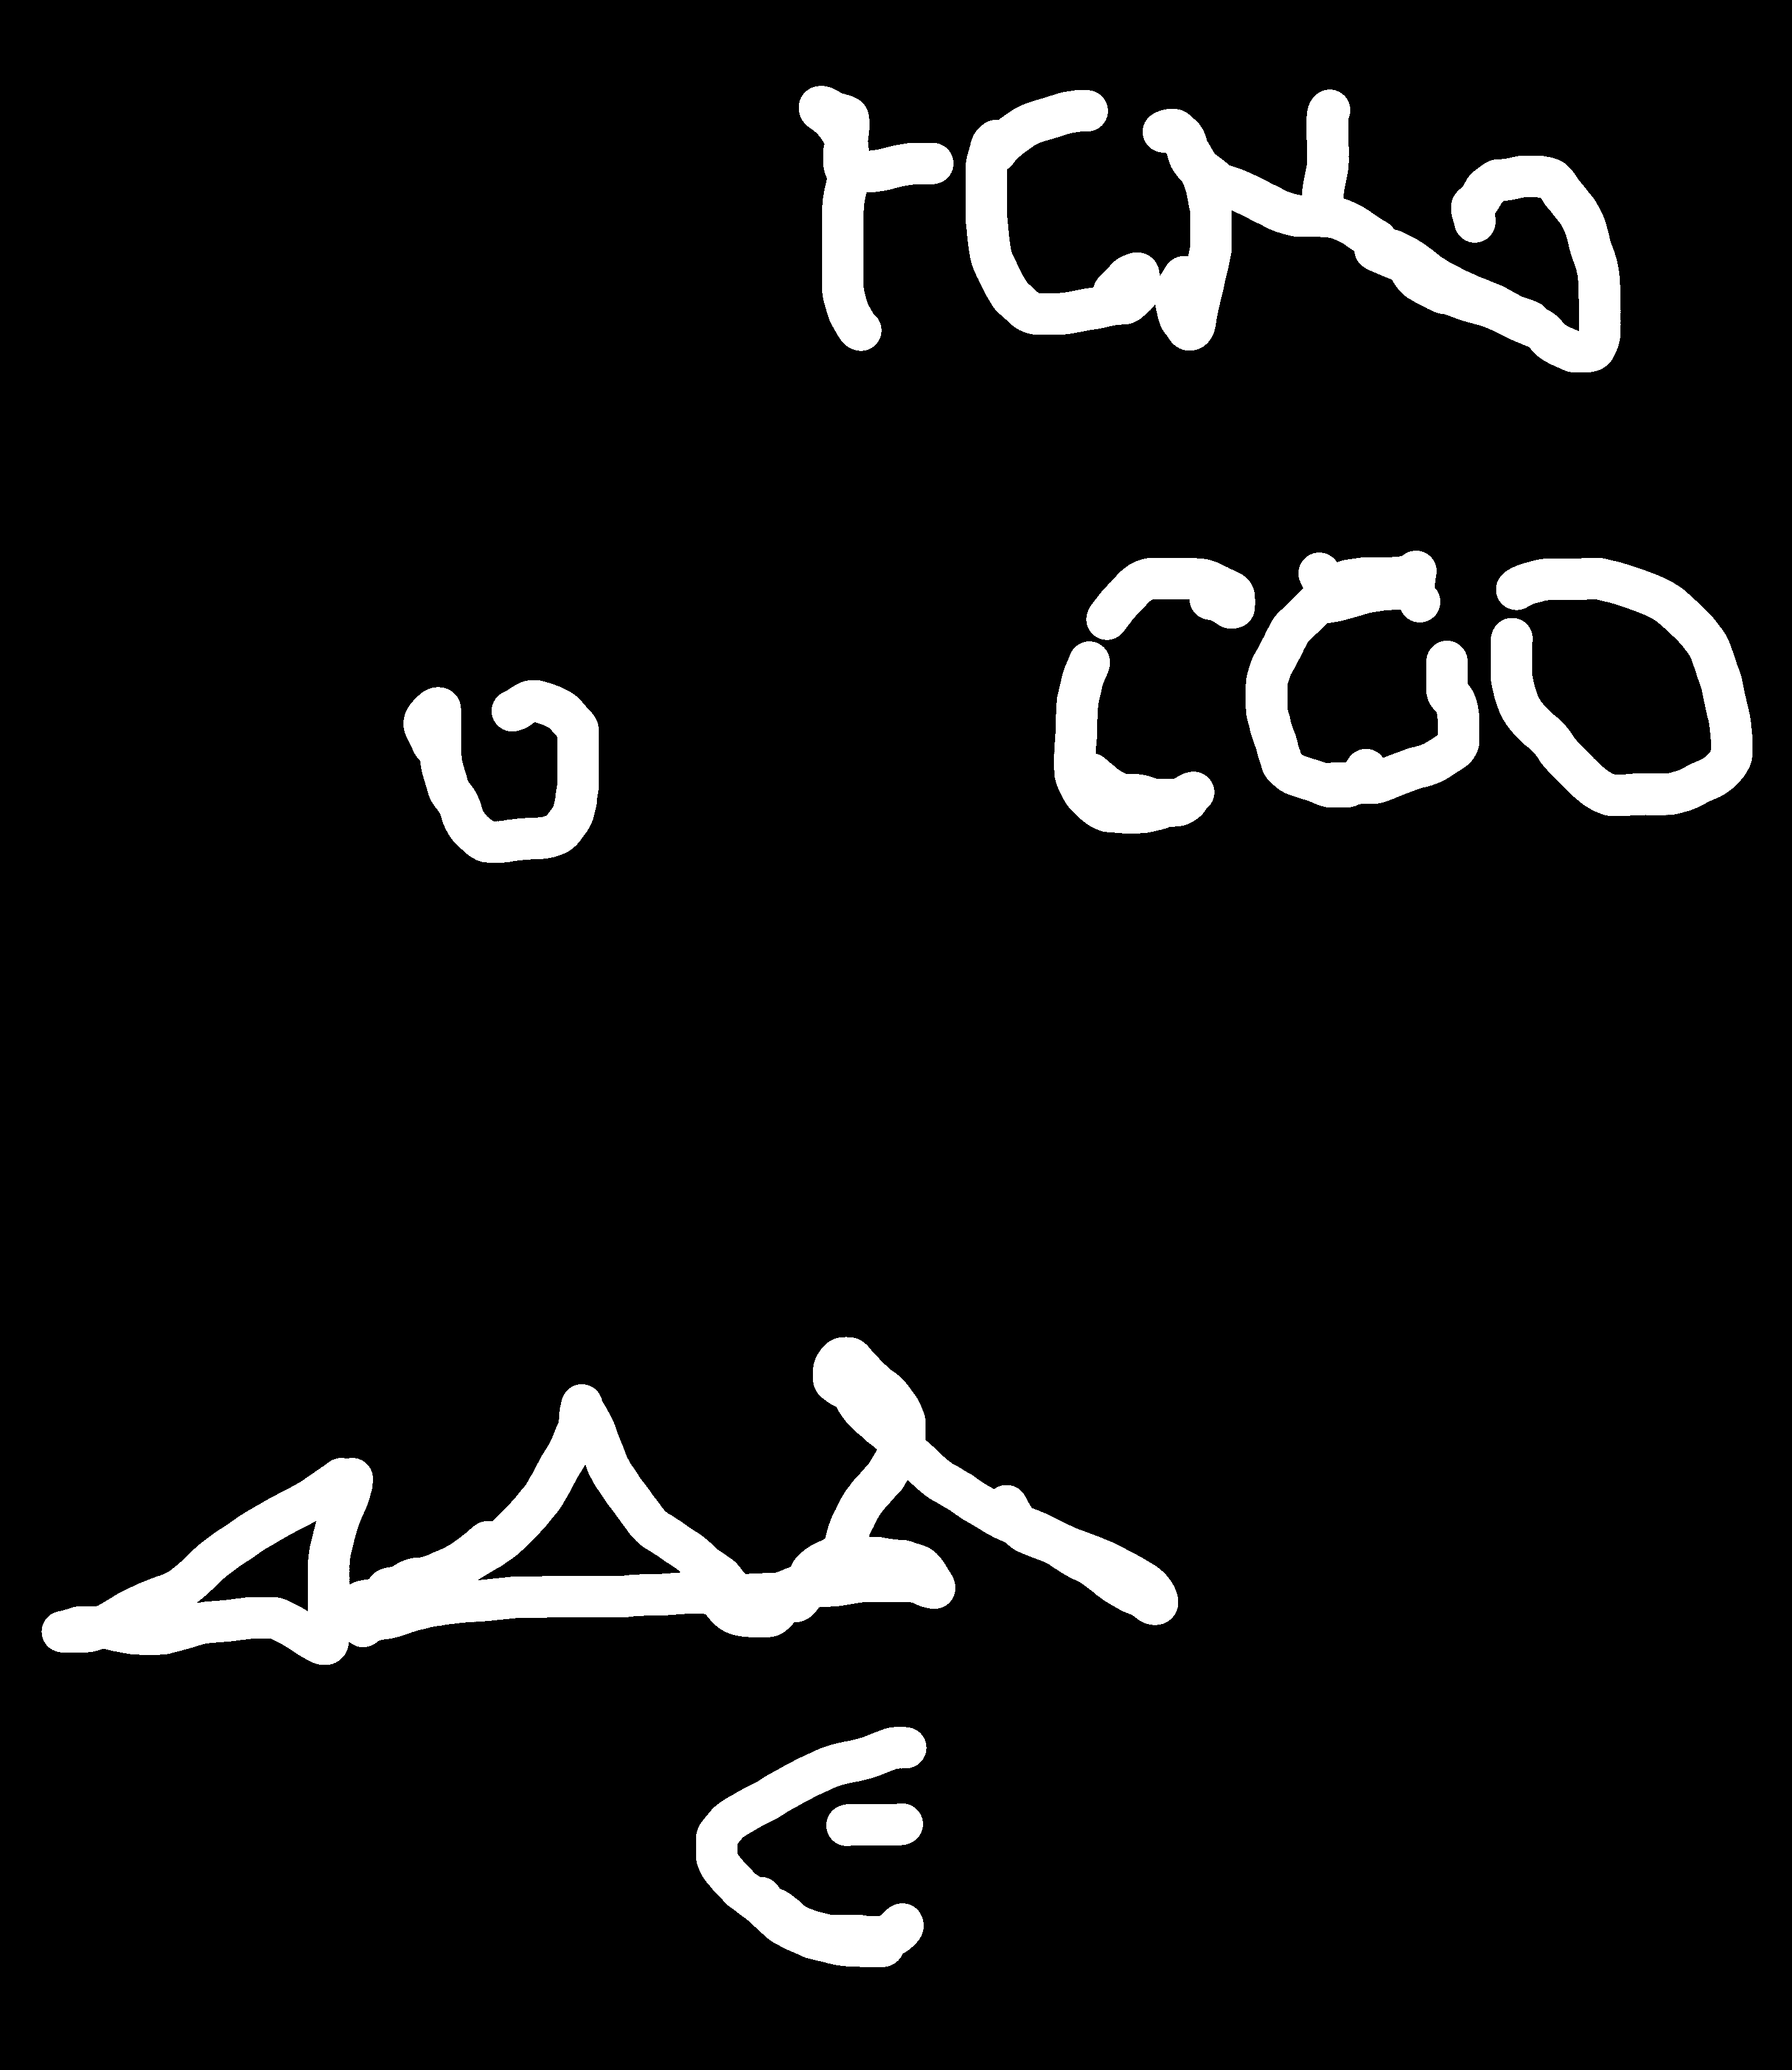
\includegraphics[width=122.48pt]{../figures/w060/w060_2_labels.png}}\end{minipage}}
\par\vspace{4pt}
\noindent\makebox[\columnwidth][c]{\begin{minipage}[t]{122.48pt}\centering\href{https://raw.githubusercontent.com/evilaliv3/vesuvius-challenge-pipeline/main/results/db27c806-rectina/src/figures/w060/w060_3_reader-v2.png}{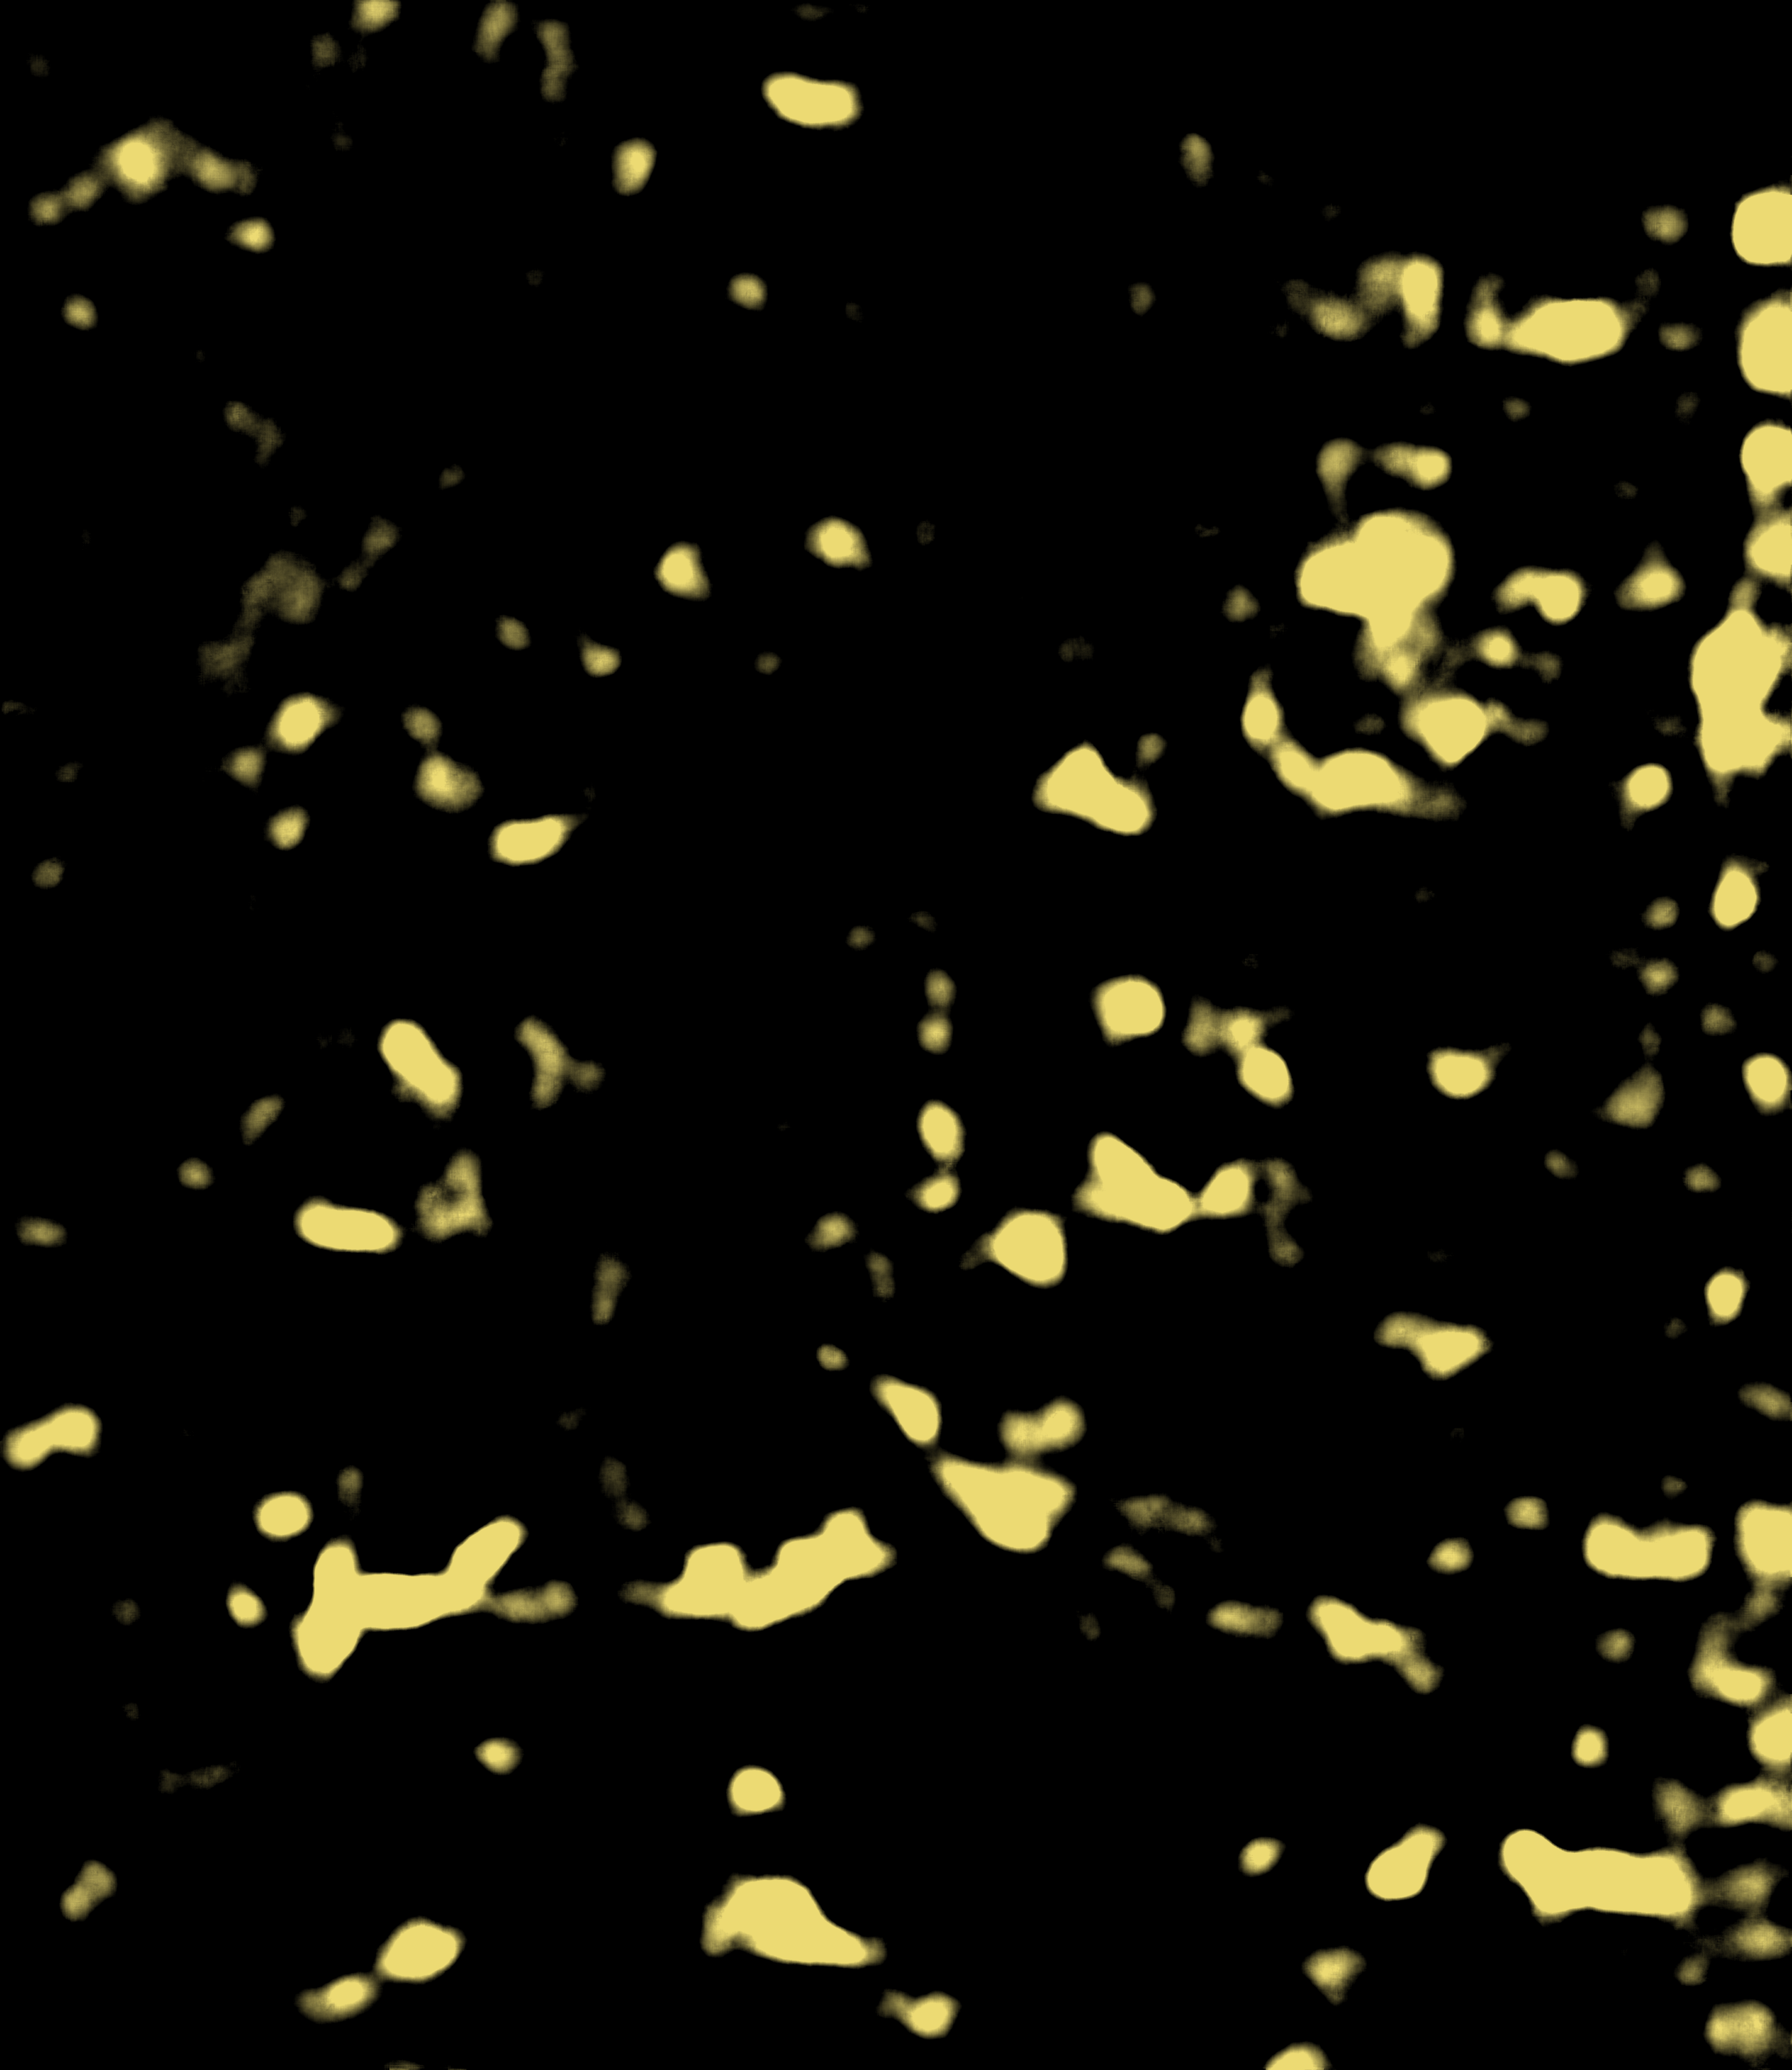
\includegraphics[width=122.48pt]{../figures/w060/w060_3_reader-v2.png}}\end{minipage}\hspace{2pt}\begin{minipage}[t]{122.48pt}\centering\href{https://raw.githubusercontent.com/evilaliv3/vesuvius-challenge-pipeline/main/results/db27c806-rectina/src/figures/w060/w060_5_rectina-m1.png}{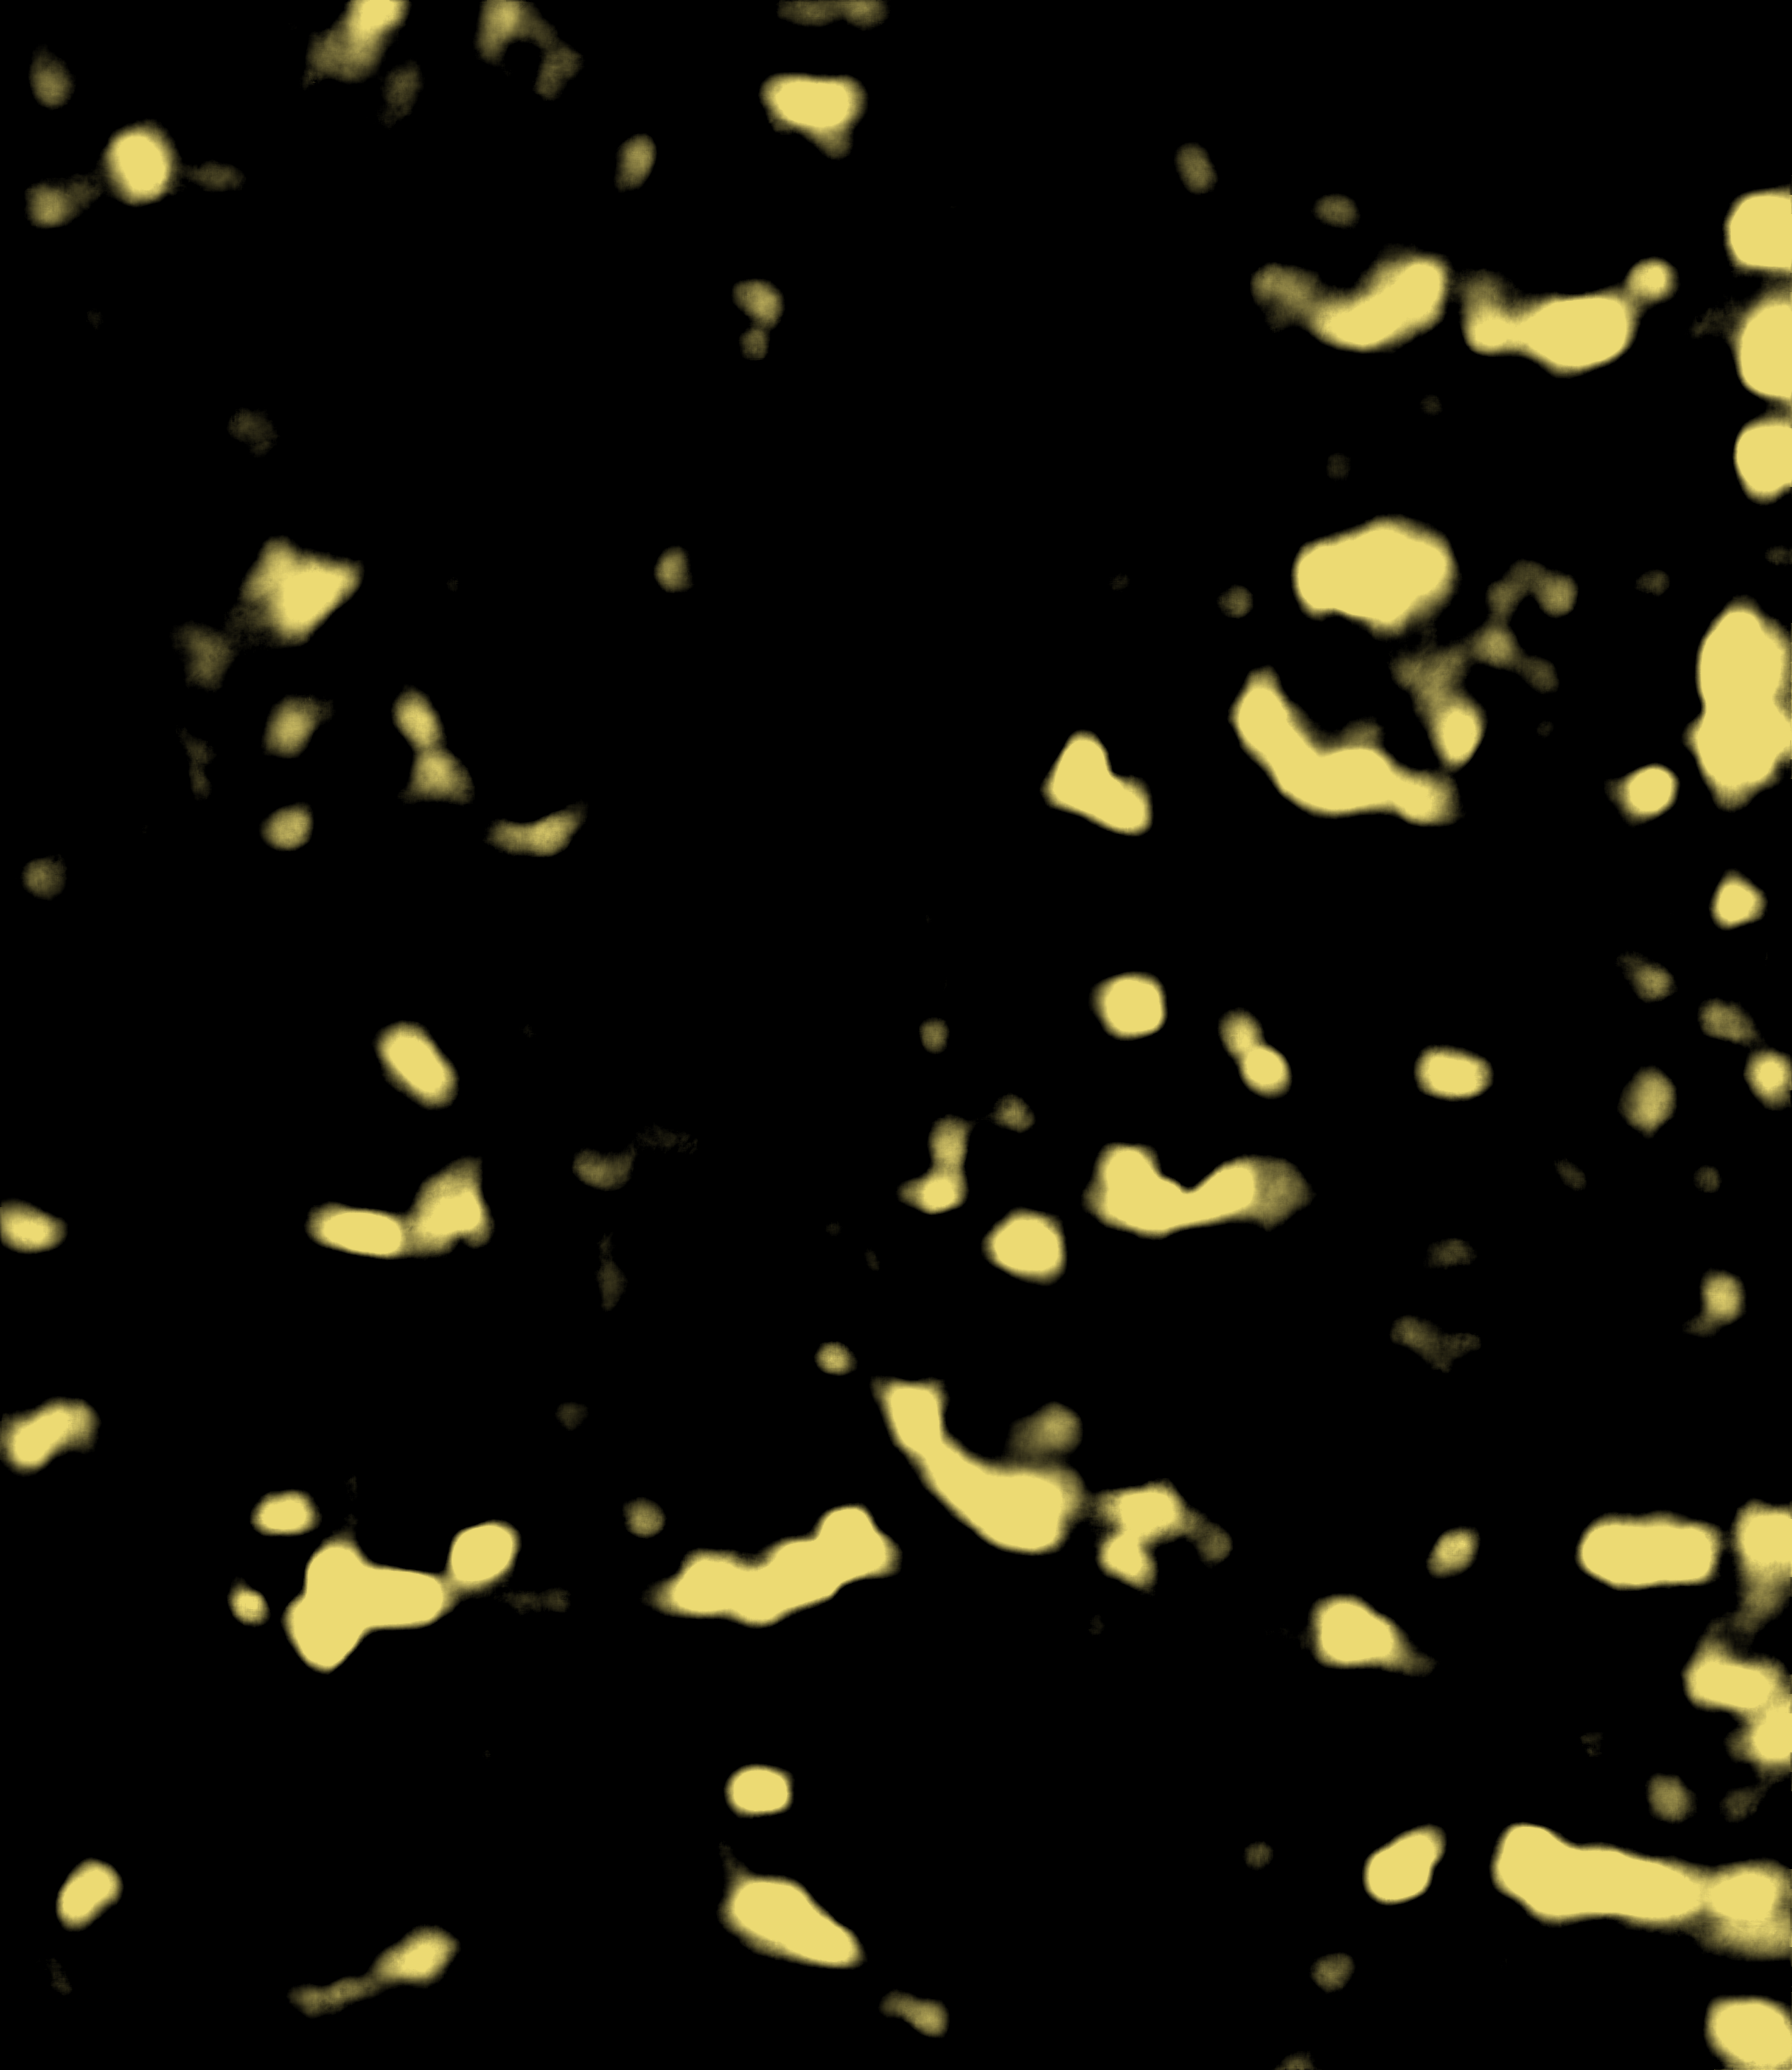
\includegraphics[width=122.48pt]{../figures/w060/w060_5_rectina-m1.png}}\end{minipage}}
\par\vspace{4pt}
\noindent\makebox[\columnwidth][c]{\begin{minipage}[t]{122.48pt}\centering\href{https://raw.githubusercontent.com/evilaliv3/vesuvius-challenge-pipeline/main/results/db27c806-rectina/src/figures/w060/w060_4_reader-v3.png}{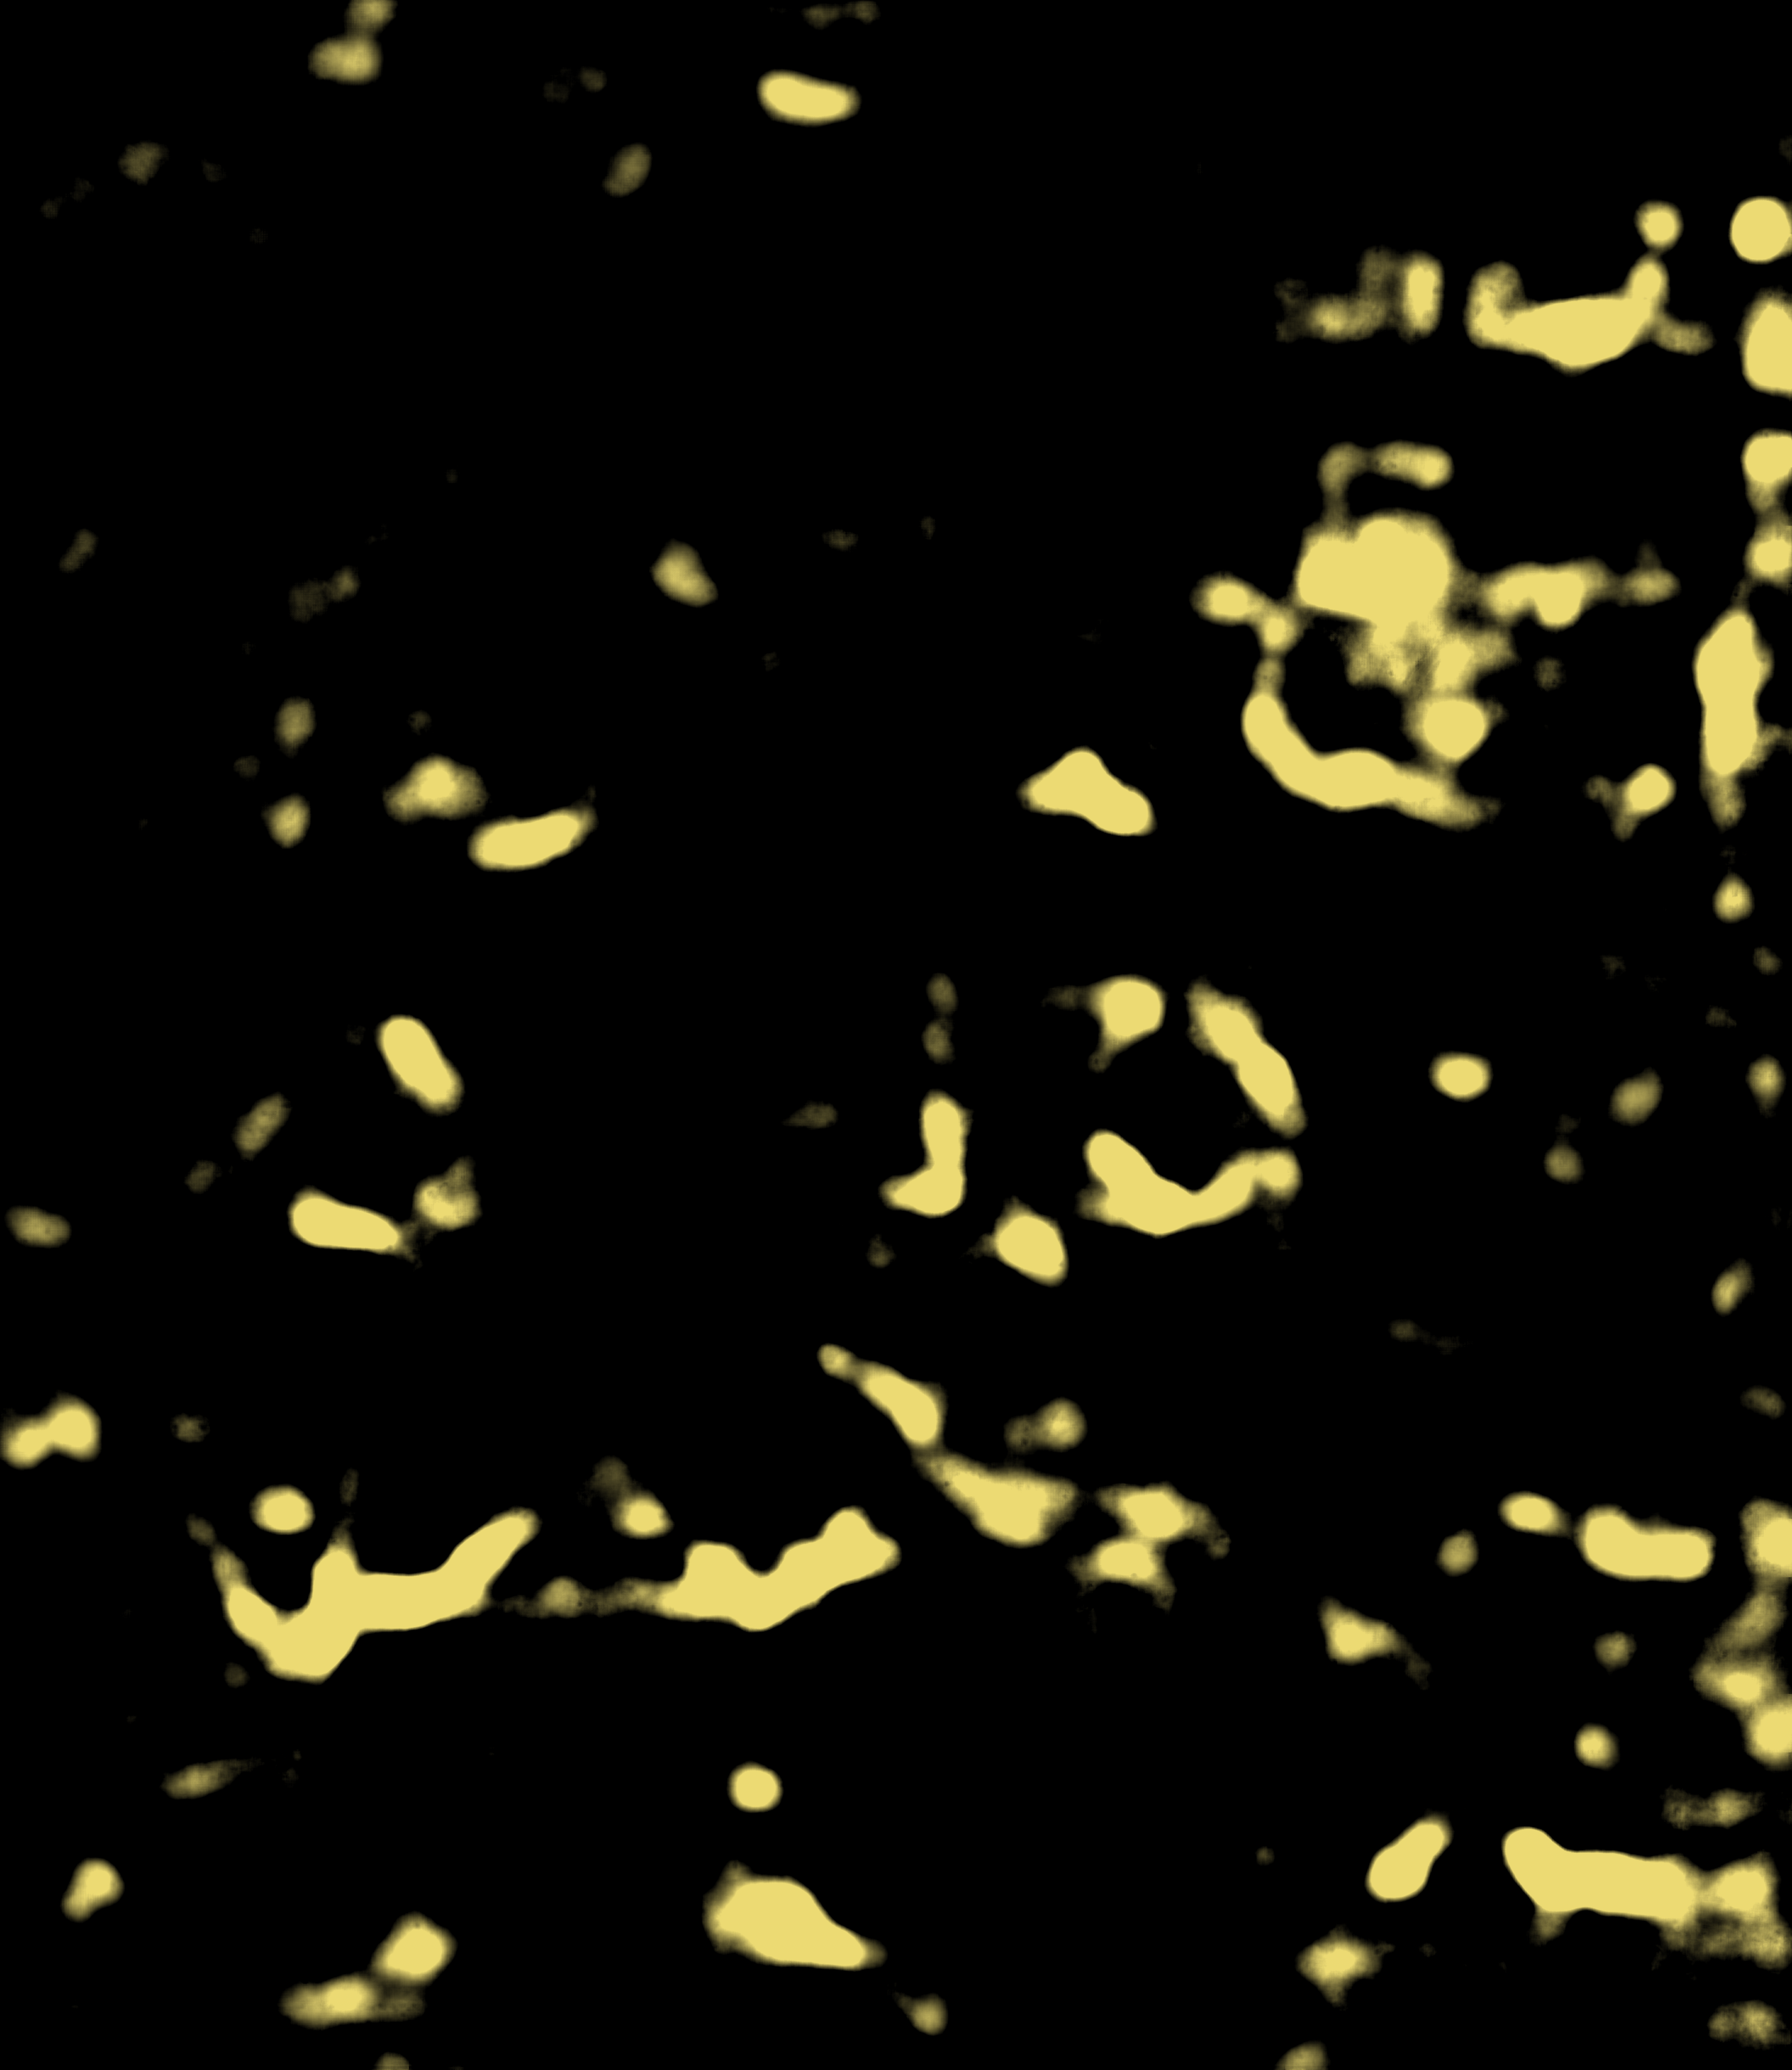
\includegraphics[width=122.48pt]{../figures/w060/w060_4_reader-v3.png}}\end{minipage}\hspace{2pt}\begin{minipage}[t]{122.48pt}\centering\href{https://raw.githubusercontent.com/evilaliv3/vesuvius-challenge-pipeline/main/results/db27c806-rectina/src/figures/w060/w060_6_rectina-m2.png}{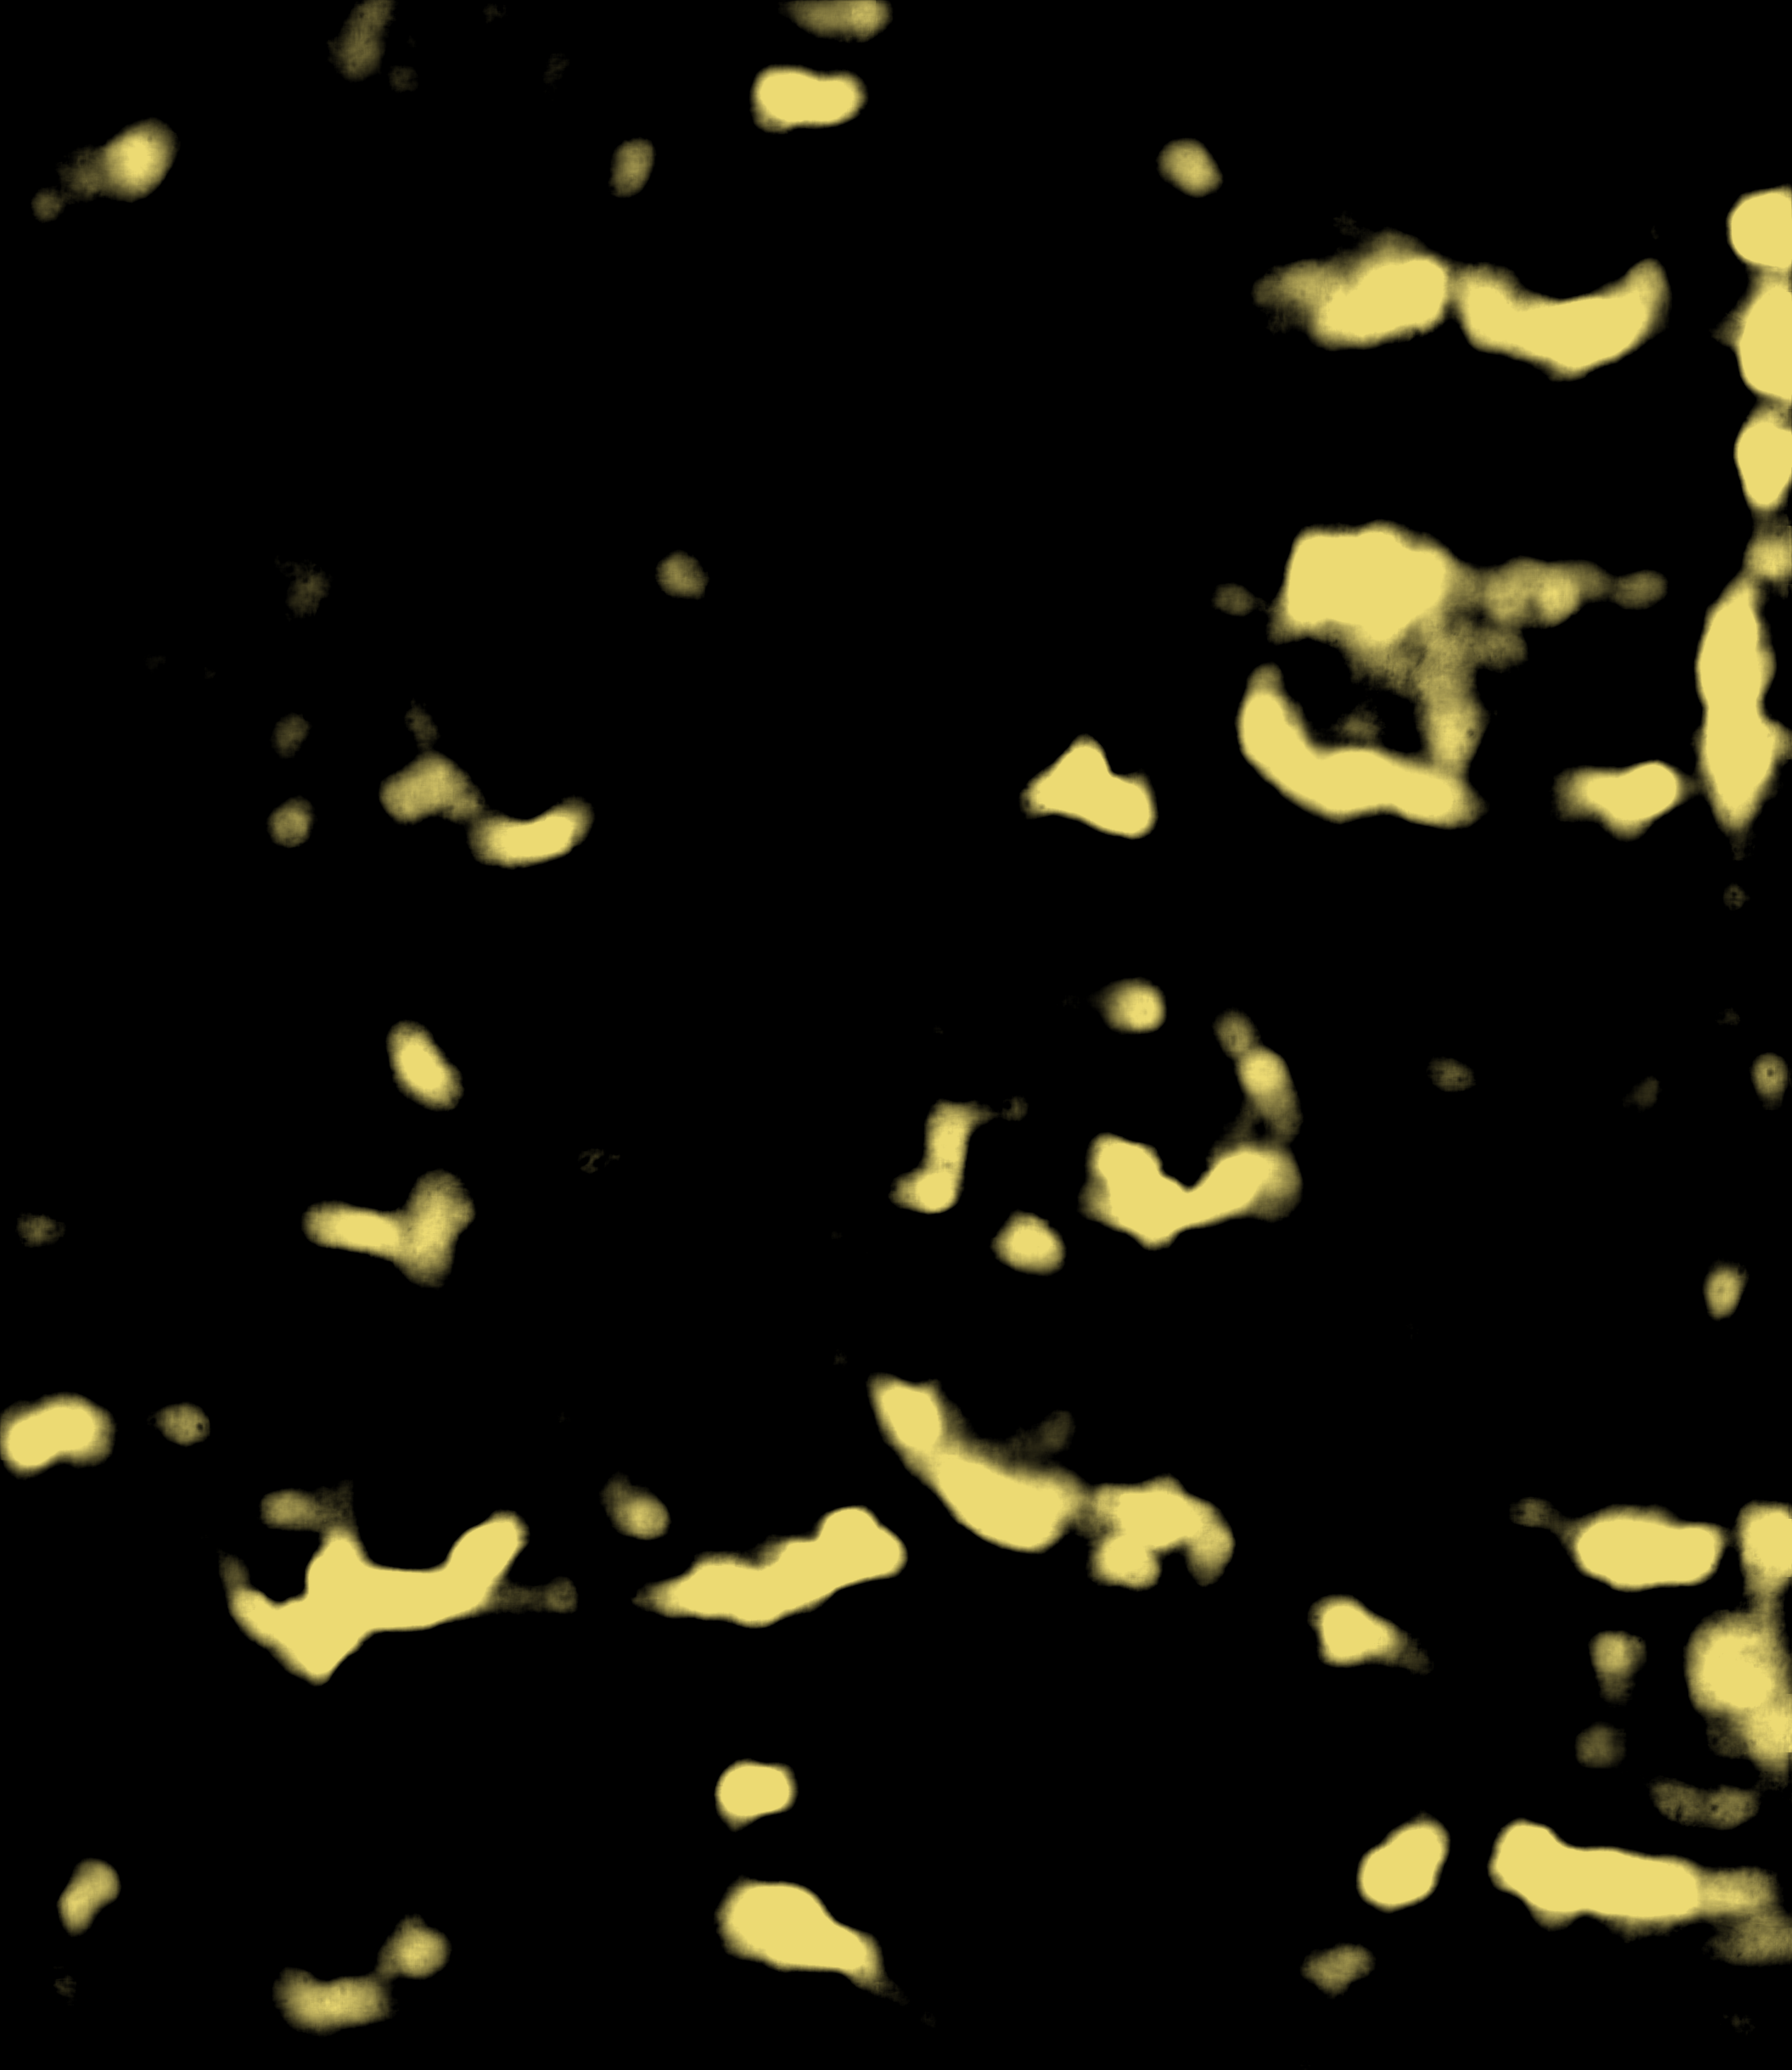
\includegraphics[width=122.48pt]{../figures/w060/w060_6_rectina-m2.png}}\end{minipage}}
\caption{Control unit 1447 w060, three rows of two panels. Row 1: left, Texture; right, Labels. Row 2: left, Reader v2; right, Rectina m1 (display windows: Reader v2 0.358837 to 0.460831 (ramp); Rectina m1 0.419819 to 0.580751 (ramp)). Row 3: left, Reader v3; right, Rectina m2 (display windows: Reader v3 0.381681 to 0.538574 (ramp); Rectina m2 0.465540 to 0.657352 (ramp)). Each map is stretched between its own percentiles. Reader and model stand side by side in the rows 2 and 3.}
\end{figure}



\section{Results for Rectina m1 against Reader v3}\label{sec:results-MB}

Rectina m1 is the checkpoint at the end of the first stage. Table~\ref{tab:comparison-MB} gives, in the format of the table of the previous section, the three measures of Reader v3 and Rectina m1 on the fourteen units.

\MBHonestSentence{}

\begin{table*}[!t]
\caption{Three measures of \MBModelName{} against Reader v3 on the fourteen units, target a: the AUC, the AUC on thin
strokes and false ink at 80 per cent recall. The cell of \MBModelName{} gives in parentheses the signed difference
against Reader v3. The rows Mean and Median are taken \MBStatScope; the
block of the community labels is information only.}\label{tab:comparison-MB}
\centering
\definecolor{rgreen}{RGB}{46,139,74}\definecolor{rred}{RGB}{192,57,43}
{\small\setlength{\tabcolsep}{2.2pt}
\noindent\begin{tabular}{>{\raggedright\arraybackslash}p{3.0cm}>{\raggedleft\arraybackslash}p{1.5cm}>{\raggedleft\arraybackslash}p{3.0cm}>{\raggedleft\arraybackslash}p{1.5cm}>{\raggedleft\arraybackslash}p{3.0cm}>{\raggedleft\arraybackslash}p{1.5cm}>{\raggedleft\arraybackslash}p{3.0cm}}
\hline
unit & \multicolumn{2}{c}{AUC} & \multicolumn{2}{c}{\shortstack{AUC on\\thin strokes}} & \multicolumn{2}{c}{\shortstack{false ink at 80\\per cent recall}} \\
 & {\footnotesize Reader v3} & {\footnotesize Rectina m1} & {\footnotesize Reader v3} & {\footnotesize Rectina m1} & {\footnotesize Reader v3} & {\footnotesize Rectina m1} \\
\hline
\multicolumn{7}{@{}p{\dimexpr 16.5cm+30.8pt\relax}@{}}{\rule{0pt}{2.6ex}\textit{Control units outside the training segments, organisers' labels: 0343 (approved letters, 116 keV); 0841 (113 keV)}} \\
0343 & 0.9078 & \textcolor{rgreen}{$\blacktriangle$}\,\textbf{0.9105} {\scriptsize (+0.0026)} & 0.9246 & 0.9246 {\scriptsize (+0.0000)} & \textbf{0.0690} & \textcolor{rred}{$\blacktriangledown$}\,0.0705 {\scriptsize (+0.0014)} \\
0841 ag1 & \textbf{0.8513} & \textcolor{rred}{$\blacktriangledown$}\,0.8395 {\scriptsize (-0.0119)} & \textbf{0.8648} & \textcolor{rred}{$\blacktriangledown$}\,0.8519 {\scriptsize (-0.0129)} & \textbf{0.2153} & \textcolor{rred}{$\blacktriangledown$}\,0.2530 {\scriptsize (+0.0376)} \\
0841 ag2 & 0.8297 & \textcolor{rgreen}{$\blacktriangle$}\,\textbf{0.8449} {\scriptsize (+0.0153)} & 0.8474 & \textcolor{rgreen}{$\blacktriangle$}\,\textbf{0.8600} {\scriptsize (+0.0126)} & 0.2681 & \textcolor{rgreen}{$\blacktriangle$}\,\textbf{0.2631} {\scriptsize (-0.0050)} \\
0841 w00 & \textbf{0.9055} & \textcolor{rred}{$\blacktriangledown$}\,0.8826 {\scriptsize (-0.0229)} & \textbf{0.9221} & \textcolor{rred}{$\blacktriangledown$}\,0.8997 {\scriptsize (-0.0223)} & \textbf{0.1444} & \textcolor{rred}{$\blacktriangledown$}\,0.1939 {\scriptsize (+0.0495)} \\
\multicolumn{7}{@{}p{\dimexpr 16.5cm+30.8pt\relax}@{}}{\rule{0pt}{2.6ex}\textit{Control unit outside the training segments, community labels, information only: 1447 (116 keV)}} \\
1447 w058 & \textbf{0.8610} & \textcolor{rred}{$\blacktriangledown$}\,0.8491 {\scriptsize (-0.0118)} & \textbf{0.8965} & \textcolor{rred}{$\blacktriangledown$}\,0.8865 {\scriptsize (-0.0100)} & \textbf{0.2665} & \textcolor{rred}{$\blacktriangledown$}\,0.2813 {\scriptsize (+0.0148)} \\
1447 w060 & 0.7842 & \textcolor{rgreen}{$\blacktriangle$}\,\textbf{0.7958} {\scriptsize (+0.0116)} & 0.8276 & \textcolor{rgreen}{$\blacktriangle$}\,\textbf{0.8429} {\scriptsize (+0.0153)} & 0.4095 & \textcolor{rgreen}{$\blacktriangle$}\,\textbf{0.3770} {\scriptsize (-0.0325)} \\
\multicolumn{7}{@{}p{\dimexpr 16.5cm+30.8pt\relax}@{}}{\rule{0pt}{2.6ex}\textit{Held-out segments of training scrolls, our validation labels: 0009B and 0343P (116 keV), 0500P2 (113 keV)}} \\
0009B$\cdot$172639 & 0.8456 & \textcolor{rgreen}{$\blacktriangle$}\,\textbf{0.9259} {\scriptsize (+0.0803)} & 0.8515 & \textcolor{rgreen}{$\blacktriangle$}\,\textbf{0.9303} {\scriptsize (+0.0788)} & 0.3114 & \textcolor{rgreen}{$\blacktriangle$}\,\textbf{0.0960} {\scriptsize (-0.2154)} \\
0009B$\cdot$125754 & 0.9562 & \textcolor{rgreen}{$\blacktriangle$}\,\textbf{0.9600} {\scriptsize (+0.0038)} & 0.9636 & \textcolor{rgreen}{$\blacktriangle$}\,\textbf{0.9663} {\scriptsize (+0.0027)} & 0.0460 & \textcolor{rgreen}{$\blacktriangle$}\,\textbf{0.0455} {\scriptsize (-0.0006)} \\
0009B$\cdot$133208 & 0.8551 & \textcolor{rgreen}{$\blacktriangle$}\,\textbf{0.8773} {\scriptsize (+0.0222)} & 0.8672 & \textcolor{rgreen}{$\blacktriangle$}\,\textbf{0.8873} {\scriptsize (+0.0201)} & 0.2774 & \textcolor{rgreen}{$\blacktriangle$}\,\textbf{0.2203} {\scriptsize (-0.0571)} \\
0009B$\cdot$140325 & \textbf{0.9040} & \textcolor{rred}{$\blacktriangledown$}\,0.8784 {\scriptsize (-0.0256)} & \textbf{0.9110} & \textcolor{rred}{$\blacktriangledown$}\,0.8860 {\scriptsize (-0.0250)} & \textbf{0.1574} & \textcolor{rred}{$\blacktriangledown$}\,0.1908 {\scriptsize (+0.0334)} \\
0500P2$\cdot$055229 & \textbf{0.8971} & \textcolor{rred}{$\blacktriangledown$}\,0.8605 {\scriptsize (-0.0366)} & \textbf{0.9074} & \textcolor{rred}{$\blacktriangledown$}\,0.8698 {\scriptsize (-0.0376)} & \textbf{0.1360} & \textcolor{rred}{$\blacktriangledown$}\,0.2854 {\scriptsize (+0.1494)} \\
0500P2$\cdot$055230 & 0.7881 & \textcolor{rgreen}{$\blacktriangle$}\,\textbf{0.7984} {\scriptsize (+0.0103)} & 0.7980 & \textcolor{rgreen}{$\blacktriangle$}\,\textbf{0.8078} {\scriptsize (+0.0098)} & 0.3998 & \textcolor{rgreen}{$\blacktriangle$}\,\textbf{0.3541} {\scriptsize (-0.0458)} \\
0343P$\cdot$233748-0 & 0.8340 & \textcolor{rgreen}{$\blacktriangle$}\,\textbf{0.8584} {\scriptsize (+0.0244)} & 0.8398 & \textcolor{rgreen}{$\blacktriangle$}\,\textbf{0.8629} {\scriptsize (+0.0231)} & 0.3059 & \textcolor{rgreen}{$\blacktriangle$}\,\textbf{0.2669} {\scriptsize (-0.0390)} \\
0343P$\cdot$172054-1 & 0.7573 & \textcolor{rgreen}{$\blacktriangle$}\,\textbf{0.7981} {\scriptsize (+0.0407)} & 0.7669 & \textcolor{rgreen}{$\blacktriangle$}\,\textbf{0.8035} {\scriptsize (+0.0366)} & 0.4336 & \textcolor{rgreen}{$\blacktriangle$}\,\textbf{0.3679} {\scriptsize (-0.0657)} \\
\hline
Mean & 0.8555 & \textcolor{rgreen}{$\blacktriangle$}\,\textbf{0.8628} {\scriptsize (+0.0073)} & 0.8706 & \textcolor{rgreen}{$\blacktriangle$}\,\textbf{0.8771} {\scriptsize (+0.0065)} & 0.2458 & \textcolor{rgreen}{$\blacktriangle$}\,\textbf{0.2333} {\scriptsize (-0.0125)} \\
\hline
Median & 0.8532 & \textcolor{rgreen}{$\blacktriangle$}\,\textbf{0.8595} {\scriptsize (+0.0062)} & 0.8660 & \textcolor{rgreen}{$\blacktriangle$}\,\textbf{0.8779} {\scriptsize (+0.0119)} & 0.2673 & \textcolor{rgreen}{$\blacktriangle$}\,\textbf{0.2580} {\scriptsize (-0.0093)} \\
\hline
\end{tabular}}

\par\smallskip
{\footnotesize\raggedrightAUC: the rank AUC of ink against blank pixels. \\
AUC on thin strokes: the rank AUC of the central 80 per cent of each stroke against blank pixels at least 207 um from any label, the band between not scored. \\
false ink at 80 per cent recall: the share of blank pixels marked as ink at the threshold that recalls 80 per cent of the ink pixels, where less is better. \\
For the controls the AUC is taken against the far negatives of the bench; for the held-out units against all blank pixels of the validation mask. \\
The better value of each pair in bold; a green triangle pointing up before \MBModelName{} where it is better, a red triangle pointing down where it is worse. \\
A pair whose two values are equal at four decimals has no bold value and no triangle.
\par}
\end{table*}

On the eight held-out units the mean score is \MBHeldMeanReader{} for Reader v3 and \MBHeldMeanModel{} for \MBModelName{}; \MBModelName{} scores above Reader v3 on \MBHeldAbove{} of the 8
units, the median difference is \MBHeldMedianDiff{} and the mean difference is \MBHeldMeanDiff{}\MBLowHeld. On the six control units \MBModelName{} scores above Reader v3 on \MBStatsCtrlKText{} with a median difference of \MBStatsCtrlMedianDiff{}. On the four controls with organisers' labels (ag1, ag2, w00, 0343), a subset of the six, the split following from who made the labels of each unit, a fact about the data and not a choice made on the scores (both counts are given because the split was not fixed before the scores), the mean score is \MBCtrlMeanReader{} for Reader v3 and \MBCtrlMeanModel{} for
\MBModelName{}; \MBModelName{} scores above Reader v3 on
\MBCtrlAbove{} of the \MBCtrlN{} units, the median difference is \MBCtrlMedianDiff{} and the mean difference is
\MBCtrlMeanDiff{}\MBLowCtrl.

\MBFalseInkParagraph{}

\MBStatsParagraph{} \MBSeedParagraph{}


\section{Usage}\label{sec:usage}

The pieces for using the checkpoints are published with this article in its results folder~\cite{ownfolder}: the reader in \UsageDirRead{}, the recipe of the render in \UsageDirRender{} and the converters of a map in \UsageDirConvert{}. This section says what each piece does and what was run and not run; the README of each folder says more.

Input. A checkpoint of Rectina reads a surface volume: a stack of layers sampled along the normal of a segmented surface, stored as an array of shape (planes, rows, columns), as an npy file or an OME-Zarr folder. The reader takes seventeen consecutive planes from the stack and slides a square patch over rows and columns. The stacks used in this work have twenty three planes, stored as uint16 holding the rendered grey value times 256, so that 65280 is the saturated value of an 8 bit render, and divided by 65280 before reading; the seven read starts are the seven windows of seventeen planes inside the twenty three. The reader applies to every patch the robust median absolute deviation normalisation of the villa ink detection code (percentiles 1 and 99). The stack has to be rendered along the surface normal at the scale of the training data, about 9 um. Reads of stacks from another render were not tested.

Reading a unit. The reader of \UsageDirRead{} is run with the villa package at the commit that its README pins (the commands of the README):

\begin{quote}
\begin{Verbatim}[fontsize=\scriptsize,breaklines=true,breakanywhere=true,breakautoindent=false]
git clone https://github.com/ScrollPrize/villa.git && git -C villa checkout 0bc2c241de7e289e36459468a9a0b32257679966
\end{Verbatim}
\end{quote}


\begin{quote}
\begin{Verbatim}[fontsize=\scriptsize,breaklines=true,breakanywhere=true,breakautoindent=false]
python3 rectina_read.py info    --checkpoint m2/ckpt_020000.pth
python3 rectina_read.py read    --stack unit.npy --checkpoint m2/ckpt_020000.pth --villa-src villa/vesuvius/src --device cuda --out out/unit
python3 rectina_read.py compare out/unit/map.npy reference_map.npy
\end{Verbatim}
\end{quote}


Each start reads its seventeen planes with two views (the identity and the view turned by 180 degrees, whose maps are averaged), four lattices shifted by a quarter of a patch, bfloat16 autocast on a graphics processor and Hann window blending; the map is the mean over the seven starts. The patch is \UsagePatchOne{} pixels for \UsageNameOne{} and \UsagePatchTwo{} pixels for \UsageNameTwo{}: it is the crop size of the configuration embedded in each checkpoint, read from the checkpoint (not inferred). A read needs a graphics processor in practice: for \UsageNameTwo{} a read of one million pixels took about \UsageSecPerMpxTwo{} seconds for the seven starts on a graphics processor of type \UsageDeviceTwo{} (peak memory \UsagePeakTwo{} MiB), and for \UsageNameOne{} about \UsageSecPerMpxOne{} seconds (peak memory \UsagePeakOne{} MiB), both read from the records of the reads of unit ag1. Run by: the author, on a rented RTX 4090 machine with bfloat16, for unit ag1 only, the commands read and compare of the README; the result is that the public reader reproduces the stored maps of the same checkpoints on this one unit (the sha256 of both maps equal the stored ones), and nothing more: it says nothing about other units, other stacks or other hardware. Also run: the comparison of a CPU read of a crop of unit ag1 with \UsageNameOne{} against the stored map, inside the declared limits. Not tested: the command info, \UsageNameTwo{} on a CPU, other graphics processors.

Output. For each unit the read writes map.npy (float32, rows by columns of the stack, values between 0 and 1), reads.csv and a record of the sha256 of the outputs. The map is a ranking score of ink against papyrus and not a calibrated probability: \UsageCalibration{} \LabelSmoothing{} On a real unit the values span a narrow band, for instance \UsageBandOne{} for \UsageNameTwo{} on ag1 and \UsageBandTwo{} on 0343, so a fixed threshold such as 0.5 means nothing; evaluate by rank (the area under the curve) or choose a threshold on a labelled region. To make an image, scale the map linearly between two percentiles and write an 8 bit tif.

Worked example. Unit ag1, a control unit of the comparison (organisers' human labels, none of its segments used in training), \UsageShapeOne{} pixels. The stored map of \UsageNameOne{} has sha256 \UsageShaOne{} and scores an area under the curve of \UsageAucOne{} (\UsageAucOneFull{}) against the labels with the scorer of this work; the stored map of \UsageNameTwo{} has sha256 \UsageShaTwo{} and scores \UsageAucTwo{} (\UsageAucTwoFull{}); both numbers are the cells of the comparison tables. Scoring a stored map needs no graphics processor. The declared limits for a map read on another device against a reference map are a largest absolute difference of \UsageTolAbs{}, a mean absolute difference of \UsageTolMean{} and a Pearson correlation of at least \UsageTolPearson{}.

Converting a map. The converter of \UsageDirConvert{} writes a map as a tif or as OME-Zarr and reads either back to check it against the npy (the commands of its README):

\begin{quote}
\begin{Verbatim}[fontsize=\scriptsize,breaklines=true,breakanywhere=true,breakautoindent=false]
python3 rectina_map_convert.py tif map.npy map_float32.tif
python3 rectina_map_convert.py tif map.npy map_uint16.tif --dtype uint16
python3 rectina_map_convert.py zarr map.npy map_v3.zarr
python3 rectina_map_convert.py zarr map.npy map_v2.zarr --zarr-format 2 --pixel-size-um 9.36
python3 rectina_map_convert.py check map.npy map_float32.tif
python3 rectina_map_convert.py check map.npy map_uint16.tif
python3 rectina_map_convert.py check map.npy map_v3.zarr
python3 rectina_map_convert.py check map.npy map_v2.zarr
\end{Verbatim}
\end{quote}


Run by: the test of that folder, on three real maps (two control units and one held-out unit): all four conversions and all four round trip checks passed. Not run: any OME-Zarr validator.

Rendering. The recipe of the render is in \UsageDirRender{}: the villa tool vc\_render\_tifxyz built from an upstream commit plus one patch of the study, with the settings of the stacks (twenty three planes at step one, float32 samples stored as uint16). It is a record of a recipe and does not replace the render component of the public chain. The binary of the original build is no longer on disk (a cleanup removed it); a rebuild from the same commit, patch and recipe has another file hash, and reproduced a stored render shard bit for bit in one reference run; the stacks of this recipe were not compared for equality with those of the public render component. Not tested: any other render of the same surface as input to the checkpoints.

Plugging in. The architecture is \texttt{\UsageArch{}} with a seventeen plane crop and \UsageTensors{} tensors. The ink detection package of villa builds it from the configuration embedded in the checkpoint (the function that makes the model, models/model.py of the package, which names this architecture). Verified by reading code only. Not tested: the inference command of that package with the checkpoints of this article, the current villa head.

What was not tested. Other renders, other scrolls than the fourteen units of the comparison, other graphics processors than the ones of the registered runs, meshes or surfaces that are not tifxyz, and scales other than the 9 um class of the training data.


\section{Upstream contributions}

The simpler rule was proposed to villa as pull request \href{https://github.com/ScrollPrize/villa/pull/2396}{2396},
opened as a draft on 31 October 2026, not part of these models. The pull requests below are those that the models
used. Each one links to its page, its state was read from the code host at the time this text was built (fetched
\MAPrFetched{}, \MAPrState{}), and the last two columns say what the change does and what role it has for the models.

\begin{table*}[!t]
\caption{The pull requests of the project that these models used.}\label{tab:pulls}
\centering
{\small\setlength{\tabcolsep}{3pt}
\noindent\begin{tabular}{@{}p{2.2cm}p{1.6cm}p{4.6cm}p{6.4cm}@{}}
\hline
item & state & what it does & role in the models \\
\hline
\href{https://github.com/ScrollPrize/villa/pull/2396}{villa 2396} & open, draft & Falls back to villa's own normalisation when a robust\_mad window is about half fill, instead of dividing by a near zero scale. & The same idea as the MAD guard of step 1, in a simpler form for villa's own normalisation; the model was trained with our guard. \\
\href{https://github.com/ScrollPrize/villa/pull/2247}{villa 2247} & open & Adds an opt in bilinear blend of node normals for linear surface interpolation. & The change equivalent to the blended normals of our render patch, which produced every render the model was trained and scored on. \\
\href{https://github.com/ScrollPrize/villa/issues/2243}{villa issue 2243} & open & grid-node offset when surfaces are moved between voxel sizes (about \MALabelOffsetHigh{} px) & found and reported by us, corrected in our labels; the code path was removed in villa pull request \href{https://github.com/ScrollPrize/villa/pull/2358}{2358} (commits \href{https://github.com/ScrollPrize/villa/pull/2358/commits/9ddd16d23c7d7585a526ae26a6aefcdd68414516}{9ddd16d23} and \href{https://github.com/ScrollPrize/villa/pull/2358/commits/c73ccbbc9e18e5062ea611692cc274d55305435d}{c73ccbbc9}) \\
\hline
\end{tabular}}

\end{table*}

The label regrid offset we found and reported in villa issue \href{https://github.com/ScrollPrize/villa/issues/2243}{2243}
was corrected in the labels used here; the code that carried it was later
removed from villa in pull request \href{https://github.com/ScrollPrize/villa/pull/2358}{2358},
so the correction needs no pull request. The month's other contributions are listed in a separate submission.

\section{Limits}

The score is our own metric, the area under the curve of a probability map against a mask, and it is not the metric
of any contest. On the held-out units it is computed on one window per unit, and the choice of the window changes
it; on the control units it is computed on the whole box. The labels of the controls are of three kinds that should
not be mixed in a reading: human labels of the organisers for ag1, ag2 and w00, the mask of the approved letters for
0343, which we know only through the announcement image and therefore only as that image shows it, and labels of the
community for w058 and w060. None of them is a reference of the same standing as the others. The 113 keV block holds
two units of a single scroll scanned at another energy than the other six, so its counts are small and support no
statement about energy. Each checkpoint was trained once, and no repeat of the training exists, so that the spread between
two runs of the same configuration is not measured here and a difference of a few thousandths between two scores must
not be read as a result. The overlap check of appendix~C finds all \MAOverlapWord{} units outside the training sets; it compares the keys of the segments, not neighbouring areas of one volume. The sources of the label set and the rule that turned them into masks are not recorded in a pinned file of this work; what is recorded is the inventory of its \MALabelUnits{} units by kind, in the inventory of the study.

\section{Release}

\MAReleaseCkpt{} The models \MAPublishVerb{} in the repository \href{https://huggingface.co/evilaliv3/rectina}{evilaliv3/rectina} on Hugging Face, Rectina m1 in the folder \href{https://huggingface.co/evilaliv3/rectina/tree/main/m1}{m1} and Rectina m2 in the folder \href{https://huggingface.co/evilaliv3/rectina/tree/main/m2}{m2}. The weights and the model cards
are released under CC BY-NC 4.0 for non-commercial research use with attribution, and the code of the recipe under
MIT. The panels, the sources and the numbers files of this article are published in its own results folder~\cite{ownfolder}, whose \UsageDirRead{}, \UsageDirRender{} and \UsageDirConvert{} hold the public reader, the recipe of the render and the converters of a map (section~\ref{sec:usage}); the checkpoints are in the model repository~\cite{hfrepo}. Data terms: the data of the Vesuvius Challenge are subject to its data licence (dl.ash2txt.org LICENSE.txt). The figure panels show the CT surface, the human ink labels of the evaluation units and the model maps, with attribution to their authors; they are published on the author's own responsibility as figures of this work. This article and its results folder hold no data volumes and no label files.

\appendices

\section{The recipe table}

\clearpage\onecolumn
{\small\setlength{\tabcolsep}{3pt}
\begin{longtable}{@{}p{2.2cm}p{4.6cm}p{5.2cm}p{4.4cm}@{}}
step & setting & value & source \\ \hline \endhead
1 s1 & stage base & villa\_\allowbreak{}hybrid & training job record \\
1 s1 & iterations (to the fixed step) & 131000 & training job record \\
1 s1 & batch (patches per step,\allowbreak{} sum of the quotas) & 64 & training job record \\
1 s1 & per-\allowbreak{}scroll quotas of the batch & \{"0139":\allowbreak{} 12,\allowbreak{} "1667":\allowbreak{} 8,\allowbreak{} "Paris4":\allowbreak{} 6,\allowbreak{} "0814":\allowbreak{} 7,\allowbreak{} "0009B":\allowbreak{} 8,\allowbreak{} "0343P":\allowbreak{} 5,\allowbreak{} "0500P2":\allowbreak{} 7,\allowbreak{} "0172":\allowbreak{} 11\} & training job record \\
1 s1 & mixed precision & fp16 & stage configuration \\
1 s1 & patch size (z,\allowbreak{} y,\allowbreak{} x) & [17,\allowbreak{} 128,\allowbreak{} 128] & stage configuration \\
1 s1 & learning rate & 0.\allowbreak{}01 & stage configuration \\
1 s1 & optimizer & sgd & stage configuration \\
1 s1 & warmup steps & 1000 & stage configuration \\
1 s1 & validation every & 1000 & training job record \\
1 s1 & depth warp augmentation max offset & 3 & training job record \\
1 s1 & checkpoint taken at the end of the step & ckpt\_\allowbreak{}130001.\allowbreak{}pth & training job record \\
2 s3 & iterations & 30000 & training job record \\
2 s3 & batch size & 10 & training job record \\
2 s3 & crop and patch size (z,\allowbreak{} y,\allowbreak{} x) & [17,\allowbreak{} 256,\allowbreak{} 256] & training job record \\
2 s3 & learning rate & 0.\allowbreak{}003 & stage configuration \\
2 s3 & keep rule & last\_\allowbreak{}step (ckpt\_\allowbreak{}030000.\allowbreak{}pth) & training job record \\
2 s3 & validation every & 2000 & training job record \\
3 s4 & iterations & 20000 & training job record \\
3 s4 & batch size & 10 & training job record \\
3 s4 & crop and patch size (z,\allowbreak{} y,\allowbreak{} x) & [17,\allowbreak{} 384,\allowbreak{} 384] & training job record \\
3 s4 & learning rate & 0.\allowbreak{}003 & stage configuration \\
3 s4 & checkpoint released & ckpt\_\allowbreak{}020000.\allowbreak{}pth (last step) & training job record \\
3 s4 & keep rule & last\_\allowbreak{}step & training job record \\
all steps & scheduler & \{"name":\allowbreak{} "diffusers\_\allowbreak{}cosine\_\allowbreak{}warmup"\} & stage configuration \\
all steps & weight\_\allowbreak{}decay & 3e-\allowbreak{}05 & stage configuration \\
all steps & seed & 42 & stage configuration \\
all steps & val\_\allowbreak{}steps & 32 & stage configuration \\
all steps & label smoothing of the BCE loss & 0.\allowbreak{}5 & stage configuration \\
all steps & validation split:\allowbreak{} tile px & 512 & training job record \\
all steps & validation split:\allowbreak{} fraction of supervised pixels & 0.\allowbreak{}05 & training job record \\
all steps & validation split:\allowbreak{} seed & 20261017 & training job record \\
all steps & label set id & 43965c9d120c & run register \\
1 s1 & villa base config:\allowbreak{} optimizer & sgd & villa@3ea17f54a9b3:\allowbreak{}ink-\allowbreak{}detection/\allowbreak{}configs/\allowbreak{}aligned21\_\allowbreak{}hybrid\_\allowbreak{}3d2d.\allowbreak{}json,\allowbreak{} line 41 \\
1 s1 & villa base config:\allowbreak{} learning rate & 0.\allowbreak{}01 & villa@3ea17f54a9b3:\allowbreak{}ink-\allowbreak{}detection/\allowbreak{}configs/\allowbreak{}aligned21\_\allowbreak{}hybrid\_\allowbreak{}3d2d.\allowbreak{}json,\allowbreak{} line 42 \\
1 s1 & villa base config:\allowbreak{} batch size & 64 & villa@3ea17f54a9b3:\allowbreak{}ink-\allowbreak{}detection/\allowbreak{}configs/\allowbreak{}aligned21\_\allowbreak{}hybrid\_\allowbreak{}3d2d.\allowbreak{}json,\allowbreak{} line 48 \\
1 s1 & villa base config:\allowbreak{} patch size (z,\allowbreak{} y,\allowbreak{} x) & [17,\allowbreak{} 128,\allowbreak{} 128] & villa@3ea17f54a9b3:\allowbreak{}ink-\allowbreak{}detection/\allowbreak{}configs/\allowbreak{}aligned21\_\allowbreak{}hybrid\_\allowbreak{}3d2d.\allowbreak{}json,\allowbreak{} line 20 \\
1 s1 & villa base config:\allowbreak{} mixed precision & fp16 & villa@3ea17f54a9b3:\allowbreak{}ink-\allowbreak{}detection/\allowbreak{}configs/\allowbreak{}aligned21\_\allowbreak{}hybrid\_\allowbreak{}3d2d.\allowbreak{}json,\allowbreak{} line 47 \\
1 s1 & resume source version (training record) & an earlier run & training job record \\
1 s1 & resume stage & s1 & training job record \\
1 s1 & iteration the resume starts at & 79001 & training job record \\
depth warp & s1 stage block:\allowbreak{} enabled & true & training job record \\
depth warp & s1 stage block:\allowbreak{} max\_\allowbreak{}offset & 3 & training job record \\
depth warp & s1 stage block:\allowbreak{} g\_\allowbreak{}range & 1 & training job record \\
depth warp & s1 stage block:\allowbreak{} amp\_\allowbreak{}max & 2 & training job record \\
depth warp & s1 stage block:\allowbreak{} sigmas\_\allowbreak{}px & [8,\allowbreak{} 16,\allowbreak{} 32,\allowbreak{} 64] & training job record \\
depth warp & s1 stage block:\allowbreak{} void\_\allowbreak{}probability & 0.\allowbreak{}05 & training job record \\
depth warp & s1 stage block:\allowbreak{} void\_\allowbreak{}px & 32 & training job record \\
depth warp & s1 registration keys (registration record of the training chain) & warp\_\allowbreak{}max\_\allowbreak{}offset=3; warp\_\allowbreak{}g\_\allowbreak{}range=2; warp\_\allowbreak{}amp\_\allowbreak{}max=2 & run register \\
depth warp & s3 registration keys (registration record of the training chain),\allowbreak{} registered but not applied:\allowbreak{} this stage has no warp block & warp\_\allowbreak{}max\_\allowbreak{}offset=3; warp\_\allowbreak{}g\_\allowbreak{}range=2; warp\_\allowbreak{}amp\_\allowbreak{}max=2 & run register \\
depth warp & s4 registration keys (registration record of the training chain),\allowbreak{} registered but not applied:\allowbreak{} this stage has no warp block & warp\_\allowbreak{}max\_\allowbreak{}offset=3; warp\_\allowbreak{}g\_\allowbreak{}range=2; warp\_\allowbreak{}amp\_\allowbreak{}max=2 & run register \\
depth warp & s3 stage override carries no flat\_\allowbreak{}z\_\allowbreak{}depth\_\allowbreak{}warp block & absent & training job record \\
depth warp & s4 stage override carries no flat\_\allowbreak{}z\_\allowbreak{}depth\_\allowbreak{}warp block & absent & training job record \\
mad guard & relative threshold MAD\_\allowbreak{}REL (scaled MAD under this fraction of the 1.\allowbreak{}.\allowbreak{}99 percentile span) & 0.\allowbreak{}01 & training hook code \\
mad guard & lower bound of the scaled MAD (below it villa's own fallback already applies) & 1e-\allowbreak{}6 & training hook code \\
mad guard & UPSTREAM pull request proposal,\allowbreak{} NOT our hook:\allowbreak{} fallback whenever the scaled MAD is under this fraction of the value span & 1e-\allowbreak{}2 & upstream pull request proposal text \\
\end{longtable}}
\twocolumn


\section{Graphics processors of the reads}

\GpuSentence{}

{\small\setlength{\tabcolsep}{4pt}
\noindent\begin{tabular}{@{}lrrrr@{}}
\hline
model & 4090 & 5090 & A100 SXM & units \\
\hline
Rectina m1 & 14 & 0 & 0 & 14 \\
Rectina m2 & 8 & 0 & 6 & 14 \\
Reader v2 & 2 & 12 & 0 & 14 \\
Reader v3 & 6 & 1 & 7 & 14 \\
\hline
\end{tabular}}


\section{Provenance}

Every number of the text is read from a table written by a tool. The scores of Rectina m1 against Reader v2: \MCProvenanceScores{}. The scores of Rectina m2 against Reader v3: \MAProvenanceScores{}. The scores of Rectina m1 against Reader v3: \MBProvenanceScores{}. The units and the
energy blocks are in \path{held-out-units.csv} of the evidence of this article, the order of the units is that of the
windows table of the bench in \path{five-model-bench/evidence}, the overlap of the controls with training is read from
\path{control-overlap.csv}, the values of the recipe from the configuration files named in the table of appendix~A, the
control panels from the index named in the sections on the controls, and the states of the pull requests from the answer
of the code host saved with its checksum at the build. The short codes of the held-out units in
the tables stand for the following unit identifiers. \MAUnitCodes{}

\begin{thebibliography}{7}
\bibitem{hfrepo} Pellerano, G., Rectina, model repository with the folders m1, m2, m3 and m4, Hugging Face, 2026. \url{https://huggingface.co/evilaliv3/rectina}.
\bibitem{rectinaone} Pellerano, G., Rectina, a dense ink reader for Herculaneum papyri trained from scratch on composite labels, results/db27c806-rectina, vesuvius-challenge-pipeline, version of 1 November 2026 (public commit e4001d6, kept in the history of this folder). \url{https://github.com/evilaliv3/vesuvius-challenge-pipeline/tree/main/results/db27c806-rectina}.
\bibitem{openproblems} Vesuvius Challenge, 2026 open problems, documentation page 37\_2026\_open\_problems of the villa repository (scrollprize.org), commit a329895ea5e9. \url{https://raw.githubusercontent.com/ScrollPrize/villa/a329895ea5e9bde78752e60dbc0a4878dd2ab909/scrollprize.org/docs/37_2026_open_problems.md} (read 2026-10-09).
\bibitem{data} Vesuvius Challenge, open data, documentation page 02\_data\_datasets of the villa repository (scrollprize.org), commit a329895ea5e9. \url{https://raw.githubusercontent.com/ScrollPrize/villa/a329895ea5e9bde78752e60dbc0a4878dd2ab909/scrollprize.org/docs/02_data_datasets.md} (read 2026-10-09).
\bibitem{readertwo} Russo, D., Reader v2, repository with the README and the checkpoint link, clone at commit 02c7b4698781. \url{https://github.com/DomRusso2/reader-v2} (read 2026-10-05).
\bibitem{readerthree} Russo, D., Reader V3, repository with the README, the training configuration and the results, clone at commit 4a9f1c633d2f. \url{https://github.com/DomRusso2/reader-v3} (read 2026-10-20).
\bibitem{villa} ScrollPrize, villa, the repository of the Vesuvius Challenge with the ink detection code (vesuvius/src/vesuvius/ink\_detection), main branch at commit 7e6b82164, read through a local clone. \url{https://github.com/ScrollPrize/villa}.
\end{thebibliography}




\section*{About the author}

Giovanni Pellerano is a computer engineer and whistleblowing hacktivist.
Co-author and Project Lead of the free and open-source software, GlobaLeaks, he
is responsible for software development and for the support of the community that has grown
around it worldwide. He is a digital rights advocate currently learning more about mainstream
generative AI development and how to resist against their various and profound harms.

He had not heard of the Vesuvius Challenge before Saturday 5 September 2026. Everything reported
in this series was done after that date, which is stated because it bounds what the work can be
assumed to rest on: no prior familiarity with the data, the tools, the community or the
literature, just a curious and hyperfocused mind joining this new journey.

\section*{Declaration of generative AI in the research and writing process}

During the preparation of this work the author used Claude Fable~5.1 and Claude Opus~5.5 (Anthropic) in order
to carry out the research and to write the article: the models read the data, wrote and ran the tools,
performed the measurements, and drafted the text. The author set the direction, supplied the domain
judgement, challenged the conclusions, reviewed and edited the content, decided what was
published, and takes full responsibility for the content of the publication.

The failure this arrangement is prone to is asserting a conclusion that no measurement supports. The
comparison in this article is therefore fixed in advance as far as it can be: the rule for reading it is
quoted from a declaration written before the scores existed, the units and the windows were fixed from the
labels before any map existed, and the table says where a measure cannot be taken instead of filling the cell.

What keeps the arrangement checkable is in the folder and not in this paragraph. Every number printed here
expands a macro of \texttt{numbers.tex}, which a tool writes from the score files of the bench, and every table
is written by the same tool: none is typed by hand, by the author or by the model.


\end{document}
